\documentclass[12pt,twoside,openright,a4paper]{book}

\usepackage{fancyhdr}
\usepackage{a4wide}
\usepackage{etoc}
\usepackage{afterpage}
\usepackage{amsfonts}
\usepackage{anyfontsize}
\usepackage{url}
\usepackage{array}
\usepackage{multicol}
\usepackage{multirow}
\usepackage{parcolumns}
\usepackage{enumitem}
\usepackage{etoolbox}
\usepackage{mdwlist}
\usepackage{tabularx}
\usepackage{mathabx}
\usepackage{numprint}
\usepackage{bigdelim}
\usepackage{hhline}
\usepackage{xfp}
\usepackage{xstring}
\usepackage{xparse}
\usepackage[table]{xcolor}
\usepackage[bottom]{footmisc}
\usepackage[nottoc,numbib]{tocbibind}
\usepackage[xparse,breakable,skins,listings]{tcolorbox}
\usepackage{hyperref}
\usepackage{microtype}
\usepackage{tikz}
\usepackage[
	a4paper,
	layout=a4paper,
	bindingoffset=0.25cm,	% offset pages to accomodate for binding
	width=17cm,				% this matches original LaTeX width, geometry makes it narrower by default
	top=3cm,				% reduce top edge, too big on default settings
	bottom=2.5cm			% page numbers should be much lower on the page
]{geometry}

% include definitions from external files (note: order of inputs is important!)
\newcommand*{\isPDF}{1}
\newcommand*{\isWIP}{1}


% ░█▀▀█ ▒█▀▀█ ▒█▀▀▀█ ▒█░▒█ ▀▀█▀▀ 
% ▒█▄▄█ ▒█▀▀▄ ▒█░░▒█ ▒█░▒█ ░▒█░░ 
% ▒█░▒█ ▒█▄▄█ ▒█▄▄▄█ ░▀▄▄▀ ░▒█░░

% general document info for simpler reuse
\newcommand{\AuthorName}{Toma\v{z}}
\newcommand{\AuthorNameSurname}{\AuthorName ~Kragelj}
\newcommand{\BookTitleMain}{ZX Spectrum Next}
\newcommand{\BookTitleSub}{Assembly Developer Guide}
\newcommand{\BookTitle}{\BookTitleMain~\BookTitleSub}
\newcommand{\BookKeywords}{zx,next,spectrum,retro,documentation,manual,guide,assembly,language,programming}


% ▒█▀▀█ ▒█▀▀▀ ▒█░░▒█ ▀█▀ ▒█▀▀▀█ ▀█▀ ▒█▀▀▀█ ▒█▄░▒█ ▒█▀▀▀█ 
% ▒█▄▄▀ ▒█▀▀▀ ░▒█▒█░ ▒█░ ░▀▀▀▄▄ ▒█░ ▒█░░▒█ ▒█▒█▒█ ░▀▀▀▄▄ 
% ▒█░▒█ ▒█▄▄▄ ░░▀▄▀░ ▄█▄ ▒█▄▄▄█ ▄█▄ ▒█▄▄▄█ ▒█░░▀█ ▒█▄▄▄█

\newcommand{\LatestYear}{2021}
\newcommand{\LatestMonthName}{November}
\newcommand{\LatestMonth}{11}
\newcommand{\LatestDay}{11}

% revision name is nicely structured variant with named month
\newcommand{\LatestRevisionName}{\LatestDay~\LatestMonthName~\LatestYear}

% revision date is "reverse domain" type that can be easily sorted in various computer lists; also suitable for git tags
\newcommand{\LatestRevisionDate}{\LatestYear-\LatestMonth-\LatestDay}


% ▒█▀▀▀ ▒█░░░ ▒█▀▀▀ ▒█▀▄▀█ ▒█▀▀▀ ▒█▄░▒█ ▀▀█▀▀ ▒█▀▀▀█ 
% ▒█▀▀▀ ▒█░░░ ▒█▀▀▀ ▒█▒█▒█ ▒█▀▀▀ ▒█▒█▒█ ░▒█░░ ░▀▀▀▄▄ 
% ▒█▄▄▄ ▒█▄▄█ ▒█▄▄▄ ▒█░░▒█ ▒█▄▄▄ ▒█░░▀█ ░▒█░░ ▒█▄▄▄█

% creates an email (obfuscated for PDF variant), Discord or Twitter user text
\newcommand{\email}[3]{\ifdefined\isPDF{\tt #1 AT #2 DOT #3}\else{\tt #1@#2.#3}\fi}
\newcommand{\discord}[1]{{\tt @#1}}
\newcommand{\twitter}[1]{{\tt @#1}}

% sets given font size for just "selected" text
\newcommand{\FontSize}[2]{\fontsize{#1}{#1}\selectfont #2}

% creates minitoc without any headers; parameters:
% - (optional) #1 boolean; if star present, no styling will be applied after TOC, otherwise default styling will be applied (which is the default)
% - (optional) #1 boolean; if present, chapter TOC is generated, otherwise not (default will create TOC)
\NewDocumentCommand{\ChapterTOC}{ o o }{
	\pagestyle{nosectionmarker}

	% if #2 is present (aka not "[]"), render TOC.
	\IfValueF{#2}{
		\etocsettocstyle{}{}	% no title
		\localtableofcontents
	}
	\thispagestyle{plain}	% simple TOC pages without headers
	
	% if #1 is present (aka not "[]"), set page style to clean
	\IfValueF{#1}{\pagestyle{clean}}
}

% we can use this for pages that are intentionally left blank
\newcommand{\IntentionallyEmpty}{
	\mbox{}
	\vfill
	\begin{center}
	This page intentionally left empty
	\end{center}
	\vfill
	\mbox{}
}

% renders "work in progress" text using current font and size.
\newcommand{\WorkInProgress}{\ifdefined\isWIP\color{red}\textbf{WORK IN PROGRESS}\fi}

% renders "work in progress" sign for use on "full screen" pages; uses \Huge font by default, but that can be changed with optional parameter
\newcommand{\WorkInProgressFullScreen}[1][\normalsize]{
	\ifdefined\isWIP
		#1
		\begin{center}
			\WorkInProgress
		\end{center}
	\fi
}

\newenvironment{changemargin}[2]{%
	\begin{list}{}{%
		\setlength{\topsep}{0pt}%
		\setlength{\leftmargin}{#1}%
		\setlength{\rightmargin}{#2}%
		\setlength{\listparindent}{\parindent}%
		\setlength{\itemindent}{\parindent}%
		\setlength{\parsep}{\parskip}%
	}%
\item[]}{\end{list}}


% ▒█▀▀█ ▒█▀▀▀█ ▒█░░░ ▒█▀▀▀█ ▒█░▒█ ▒█▀▀█ ▒█▀▀▀█ 
% ▒█░░░ ▒█░░▒█ ▒█░░░ ▒█░░▒█ ▒█░▒█ ▒█▄▄▀ ░▀▀▀▄▄ 
% ▒█▄▄█ ▒█▄▄▄█ ▒█▄▄█ ▒█▄▄▄█ ░▀▄▄▀ ▒█░▒█ ▒█▄▄▄█

\definecolor{PrintableLightGray}{rgb}{0.85, 0.85, 0.85}
\definecolor{PrintableLightMidGray}{rgb}{0.7675, 0.7675, 0.7675}
\definecolor{PrintableMidGray}{rgb}{0.675, 0.675, 0.675}
\definecolor{PrintableDarkGray}{rgb}{0.5, 0.5, 0.5}


% ▒█▀▀▀█ ▒█░▒█ ▒█▀▀▀█ ▒█▀▀█ ▀▀█▀▀ ▒█░▒█ ░█▀▀█ ▒█▄░▒█ ▒█▀▀▄ ▒█▀▀▀█ 
% ░▀▀▀▄▄ ▒█▀▀█ ▒█░░▒█ ▒█▄▄▀ ░▒█░░ ▒█▀▀█ ▒█▄▄█ ▒█▒█▒█ ▒█░▒█ ░▀▀▀▄▄ 
% ▒█▄▄▄█ ▒█░▒█ ▒█▄▄▄█ ▒█░▒█ ░▒█░░ ▒█░▒█ ▒█░▒█ ▒█░░▀█ ▒█▄▄▀ ▒█▄▄▄█

% less tall slash
\newcommand\scslash{\stretchrel*{$/$}{\textsc{e}}}

% couple shorthands that can be used throughout the document
\newcommand{\Deg}{\textsuperscript{o}}
\newcommand{\ddd}{\makebox[1em][c]{.\hfil.\hfil.}}
\newcommand{\See}[1]{\textsuperscript{#1}}
\newcommand{\UNDOC}{\textnormal{\textsuperscript{**}}}
\newcommand{\ZXN}{\textnormal{\textsuperscript{ZX}}}
\newcommand{\ZXNS}{\tiny\textnormal{\textsuperscript{ZX}}}
\newcommand{\High}{\textsubscript{h}}
\newcommand{\Low}{\textsubscript{l}}

% instruction flags definitions - for unified formatting
\newcommand{\FS}{$\updownarrow$} % standard effect
\newcommand{\FN}{-}				% no effect
\newcommand{\FU}{?}				% unknown effect
\newcommand{\FX}{$\bullet$}		% special case
\newcommand{\FPV}{VF}			% PV=Overflow
\newcommand{\FPP}{PF}			% PV=Parity

% PortNoLink is short link to port with description and address, suitable for inline use. It doesn't create hyperlink though, so suitable for ports that are not described.
\newcommand{\PortNoLink}[2]{{\small \textbf{#1} \MemAddr{#2}}}
% PortLink is short link to port with description and address, suitable for inline use. It automatically embeds the whole text within hyperlink to the port with the same name.
\newcommand{\PortLink}[2]{\hyperref[#1]{\PortNoLink{#1}{#2}}}
% PortReference is longer reference with chapter title and section number mostly used for register lists when referring to previously described register.
\newcommand{\PortReference}[2]{
	\vspace*{-2ex}
	See description under section \ref{#1}, #2.
}

% PortTitle creates a title with label for the given port/register (use PortLink to refer back to the same named register)
\newcommand{\PortTitle}[2]{#1 \MemAddr{#2}\label{#1}}
% PortTitleLink is also used for titles, but where title itself functions as mention and links to the actual port/register description in another section (similar to \PortLink in this sense, but while PortLink isn't usable in the context of \subsection, PortTitleLink is!)
\newcommand{\PortTitleLink}[2]{\protect\hyperref[#1]{#1 \MemAddr{#2}}}

% generic renderer for any chip pin label (uses line above); this is used for all concrete chip labels internally.
\newcommand{\NoLinkChipPinLabel}[1]{$\mathtt{\overline{#1}}$}
% renders the given Z80 chip pin label with link to Z80 chip diagram. Needless to say - only use for links to Z80 chip pins!
\newcommand{\ZilogPinLabel}[1]{\hyperref[z80_pin_descriptions]{\NoLinkChipPinLabel{#1}}}
% renders the given DMA chip pin label with link to DMA chip diagram (once we actually have it)
\newcommand{\DMAPinLabel}[1]{\NoLinkChipPinLabel{#1}}

% other commonly used definitions
\newcommand{\MemAddr}[1]{{\tt \$#1}}


% ▒█▀▀█ ▒█▀▀▀█ ▒█▀▄▀█ ▒█▀▄▀█ ▒█▀▀▀█ ▒█▄░▒█   ▒█▀▀▄ ▒█▀▀█ ░█▀▀█ ▒█░░▒█ ░█▀▀█ ▒█▀▀█ ▒█░░░ ▒█▀▀▀ ▒█▀▀▀█ 
% ▒█░░░ ▒█░░▒█ ▒█▒█▒█ ▒█▒█▒█ ▒█░░▒█ ▒█▒█▒█   ▒█░▒█ ▒█▄▄▀ ▒█▄▄█ ▒█▒█▒█ ▒█▄▄█ ▒█▀▀▄ ▒█░░░ ▒█▀▀▀ ░▀▀▀▄▄ 
% ▒█▄▄█ ▒█▄▄▄█ ▒█░░▒█ ▒█░░▒█ ▒█▄▄▄█ ▒█░░▀█   ▒█▄▄▀ ▒█░▒█ ▒█░▒█ ▒█▄▀▄█ ▒█░▒█ ▒█▄▄█ ▒█▄▄█ ▒█▄▄▄ ▒█▄▄▄█

% horizontal arrows of arbitrary size (lehgth specified through parameter)
\newcommand{\RArrow}[1]{\parbox{#1}{\tikz{
	\draw[->,line width=0.5pt](0,0)--(#1,0);
}}}
\newcommand{\LArrow}[1]{\parbox{#1}{\tikz{
	\draw[<-,line width=0.5pt](0,0)--(#1,0);
}}}

% horizontal arrows with vertical line on the arrow side; parameters:
% - mandatory horizontal line width
% - optional any additional horizontal line styles (dotted, dashed etc)
% - optional vertical line height (divided by 2), default 0.1
% - optional arrow scale, default 1
% - optional line width, default 0.5pt
\NewDocumentCommand{\RArrowLine}{ m O{} O{0.1} O{1.6} O{0.5pt} }{\parbox{#1}{\tikz{
	\draw[-{>[scale=#4,length=#4,width=#4]},line width=#5,#2](0,0)--(#1,0);
	\draw[line width=#5](#1,-#3)--(#1,#3);
}}}
\NewDocumentCommand{\LArrowLine}{ m O{} O{0.1} O{1.6} O{0.5pt} }{\parbox{#1}{\tikz{
	\draw[line width=#5](0,-#3)--(0,#3);
	\draw[-{>[scale=#4,length=#4,width=#4]},line width=#5,#2](#1,0)--(0,0);
}}}


% ▒█▀▀█ ▒█░▒█ ▒█▀▀▀█ ▀▀█▀▀ ▒█▀▀▀█ ▒█▀▄▀█ ▀█▀ ▒█▀▀▀█ ░█▀▀█ ▀▀█▀▀ ▀█▀ ▒█▀▀▀█ ▒█▄░▒█ ▒█▀▀▀█ 
% ▒█░░░ ▒█░▒█ ░▀▀▀▄▄ ░▒█░░ ▒█░░▒█ ▒█▒█▒█ ▒█░ ░▄▄▄▀▀ ▒█▄▄█ ░▒█░░ ▒█░ ▒█░░▒█ ▒█▒█▒█ ░▀▀▀▄▄ 
% ▒█▄▄█ ░▀▄▄▀ ▒█▄▄▄█ ░▒█░░ ▒█▄▄▄█ ▒█░░▒█ ▄█▄ ▒█▄▄▄█ ▒█░▒█ ░▒█░░ ▄█▄ ▒█▄▄▄█ ▒█░░▀█ ▒█▄▄▄█

% define the style for lstlisting
\lstdefinestyle{CodeStyle}{
	basicstyle=\ttfamily\small,
	commentstyle=\color{PrintableDarkGray},
	columns=flexible,
	tabsize=4,
	numbers=left,
	numberstyle=\ttfamily\tiny,
	numbersep=1.8em,
	morecomment=[l]{;},
	moredelim=[is][\rmfamily\itshape]{|}{|},	% any text within |...| will be roman/italic
	literate={&}{\$}1							% replace `&` with `$` (to avoid syntax higlight issues)
			{Band}{\&~}1						% replace `Band` with `&` (to allow bitwise and output without & being consumed for $ from previous rule)
			{Bor}{|~}1							% replace `Bor' with `|` (to allow bitwise or output without | being consumed for roman/italic from moredelim rule above)
}

% define default settings for all tcolorbox instances
\tcbset{
	arc=4pt,			% radius for rounded corners
	boxrule=0pt,		% no frame around the box
	boxsep=1.3ex,		% add some spacing between frame and content
	left=0ex,			% left side should be flush with content
	right=0ex,			% right side should be flush with content
	top=-1.5ex,			% less spacing between frame and start of content
	bottom=-1.5ex,		% less spacing between end of content and frame
	pad at break=1pt,	% leave some small spacing between content and frame when page break occurs
	before skip=2ex,
	after skip=3ex,
	colback=PrintableLightGray,
	colframe=PrintableLightGray,
	enhanced,			% only use rounded corners on top and bottom part, not between page breaks
	breakable,			% allow breaking tcolorbox to multiple pages
	listing only,		% only show listing
	listing options={style=CodeStyle},
}

% this must be included **after** defines.tex!

% ▒█▀▀█ ░█▀▀█ ▒█▀▀█ ▒█░▄▀ ░█▀▀█ ▒█▀▀█ ▒█▀▀▀ ▒█▀▀▀█ 
% ▒█▄▄█ ▒█▄▄█ ▒█░░░ ▒█▀▄░ ▒█▄▄█ ▒█░▄▄ ▒█▀▀▀ ░▀▀▀▄▄ 
% ▒█░░░ ▒█░▒█ ▒█▄▄█ ▒█░▒█ ▒█░▒█ ▒█▄▄█ ▒█▄▄▄ ▒█▄▄▄█

\usetikzlibrary{
	matrix,
	fit,
	positioning,
	calc,
	arrows,
	arrows.meta,
	decorations.pathreplacing,
	shapes.multipart
}

\hypersetup{
	pdftitle={\BookTitle},
	pdfsubject={\BookTitle},
	pdfauthor={\AuthorNameSurname},
	pdfkeywords={\BookKeywords},
	pdfborderstyle={/W 0},	% don't use borders
	colorlinks=false,		% don't use colors for links
	linktoc=all				% link TOC
}

% ▒█▀▀█ ░█▀▀█ ▒█▀▀█ ▒█▀▀▀   ▒█▀▀▀ ▒█▀▀▀█ ▒█▀▀█ ▒█▀▄▀█ ░█▀▀█ ▀▀█▀▀ ▀▀█▀▀ ▀█▀ ▒█▄░▒█ ▒█▀▀█ 
% ▒█▄▄█ ▒█▄▄█ ▒█░▄▄ ▒█▀▀▀   ▒█▀▀▀ ▒█░░▒█ ▒█▄▄▀ ▒█▒█▒█ ▒█▄▄█ ░▒█░░ ░▒█░░ ▒█░ ▒█▒█▒█ ▒█░▄▄ 
% ▒█░░░ ▒█░▒█ ▒█▄▄█ ▒█▄▄▄   ▒█░░░ ▒█▄▄▄█ ▒█░▒█ ▒█░░▒█ ▒█░▒█ ░▒█░░ ░▒█░░ ▄█▄ ▒█░░▀█ ▒█▄▄█

% added these as compiler was complaining about too small margins; doesn't seem to change anything visually, but if compiler is happier, then I'm so too :)
\setlength{\headheight}{14.49998pt}
\addtolength{\topmargin}{-2.49998pt}

% define default paragraph styles
\setlength{\parindent}{0em}
\setlength{\parskip}{1.5ex}

% add sub-sub-sub-section and sub-sub-sub-sub-section commands!
\makeatletter
\newcommand\subsubsubsection{\@startsection{paragraph}{4}{\z@}{-0.5ex\@plus -0ex \@minus -.01ex}{.01ex \@plus .25ex}{\normalfont\normalsize\bfseries}}
\newcommand\subsubsubsubsection{\@startsection{subparagraph}{5}{\z@}{-0.5ex\@plus -0ex \@minus -.01ex}{.01ex \@plus .25ex}{\normalfont\small\bfseries}}
\makeatother

% redefine the default "plain" pagestyle (used by chapter pages)
% only show page number
\fancypagestyle{plain}{
	\fancyhf{} 
	\fancyhead{}
	\fancyhead[C]{\sffamily\footnotesize\WorkInProgress}
	\fancyfoot[LO,RE]{\sffamily\footnotesize\thepage}
	\fancyfoot[C]{\sffamily\footnotesize\WorkInProgress}
	\renewcommand{\headrulewidth}{0pt}
	\renewcommand{\footrulewidth}{0pt}
}

% define style used for normal pages
% odd pages (aka left) shows chapter marker
% even pages (aka right) shows section name
\fancypagestyle{clean}{
	\fancyhf{}
	\fancyhead[RO,LE]{\sffamily\footnotesize\WorkInProgress}
	\ifdefined\isPDF
		\fancyhead[LO,RE]{\sffamily\footnotesize\leftmark}
	\else
		\fancyhead[LO]{\sffamily\footnotesize\leftmark}
		\fancyhead[RE]{\sffamily\footnotesize\rightmark}
	\fi
	\fancyfoot[RE,LO]{\sffamily\footnotesize\thepage}
	\fancyfoot[C]{\sffamily\footnotesize\WorkInProgress}
	\renewcommand{\headrulewidth}{0.1pt}
	\renewcommand{\footrulewidth}{0pt}
}

% define style used for pages where section mark doesn't make sense
% odd and even pages show chapter marker on the outer edge
\fancypagestyle{nosectionmarker}{
	\fancyhf{}
	\fancyhead[RO,LE]{\sffamily\footnotesize\WorkInProgress}
	\fancyhead[RE,LO]{\sffamily\footnotesize\leftmark}
	\fancyfoot[RE,LO]{\sffamily\footnotesize\thepage}
	\fancyfoot[C]{\sffamily\footnotesize\WorkInProgress}
	\renewcommand{\headrulewidth}{0.1pt}
	\renewcommand{\footrulewidth}{0pt}
}

% empty pages before chapters should use empty style (aka nothing)
\let\mtcleardoublepage\cleardoublepage
\renewcommand{\cleardoublepage}{\clearpage{\pagestyle{empty}\mtcleardoublepage}}

% section marker should only use name, without number
\renewcommand{\sectionmark}[1]{\uppercase{\markright{#1}}}

% -------------------------------------------------------------------------
% couple main page formats - used in main tex file where needed; mainly to avoid having to implement this within individual chapter files which would be much less readable and more prone to issues should the order change in the future. But also makes main file more consistent and understandable; even though some of the macros are simple one lines

% format for first couple pages
\newcommand{\SetupPageFormattingTitle}{
	% use arabic numerals for starting pages
	\frontmatter

	% use empty style for first couple pages (no headers or footers), until defined otherwise
	\pagestyle{empty}
}

\newcommand{\SetupPageFormattingIntro}{
	% LaTeX assumes document starts with an odd page, however in our case the first page is an even page (the right side, then second one will be printed on the back of the same paper). This is how lulu expects it. However, since we use asymmetrical horizontal margins (to accomodate binding), leaving defaults would render the pages the other way ("inner" side where binding is would use smaller margin). It's interesting that only intro pages are affected, TOC and content is fine, even though pages are layed out the same ¯\_(ツ)_/¯ I didn't figure this one out, so am using a hack in manually setting up horizontal margins for intro pages (title is fine, text is right aligned and doesn't wrap so it naturally fits to odd page). However this messes up head rules for content pages which are not rendered the whole width of the page. To compensate we must call `\restoregeometry` before laying out the rest of the document.
	
	% Note: interestingly `\restoregeometry` produces correct results for content pages, even though they are still odd/even in the same "way" as intro pages, not sure why this custom margins are needed here!?

	% Note: we could of course add an empty page in front of the title which would eliminate this whole hacking. But we'd need to remember to remove it from generated PDF before uploading to lulu. And this is something I'm afraid I would too easily forget. The result would be very bad layout in printed book. So I prefer using the hack...

	% Note: the same left/right margin works find for odd and even pages as twopage formatter reverses margins when crossing page boundaries. These margins are larger than the rest of the document, but that's fine as intro pages show very little content.
	\newgeometry{left=3cm,right=2cm}
}

% format for TOC pages, after intro
\newcommand{\SetupPageFormattingTOC}{
	% this prevents empty page from being inserted before TOC (by default LaTeX will start chapters on odd pages which is fine for all pages except TOC - we have acknowlegements here instread)
	\let\cleardoublepage\clearpage

	% restore geometry to the one from `usepacakge` at the top of main file; this is needed to reset custom horizontal marings set for intro pages
	\restoregeometry
	
	% start numbering from 1 with TOC
	\setcounter{page}{1}

	% TOC should only display up to depth 1 (chapter+section)
	\ifdefined\isPDF
		\setcounter{tocdepth}{2}
	\else
		\setcounter{tocdepth}{1}
	\fi

	% use plain page style with just page number for following pages
	\pagestyle{plain}
}

% foramt for the book content pages, after TOC
\newcommand{\SetupPageFormattingBook}{
	% use arabic numerals for page numbers and clean page style for the rest of the document
	\mainmatter

	% we should only include sections for chapter mini-TOCs; this is only needed for non-print builds where we increase tocdepth to 2 for main TOC. But it doesn't hurt to include for both builds
	\setcounter{tocdepth}{1}

	% use default page style for all content pages
	\pagestyle{clean}
}

% format for instruction pages
\newcommand{\SetupPageFormattingInstructions}{
	% instruction pages should show chapter name on both odd & even
	\pagestyle{nosectionmarker}
}

\newcommand{\SetupPageFormattingAppendix}{
	% all chapters from hereon should be marked as appendix
	\appendix

	% only print chapters in appendices, not sections and subsections
	\addtocontents{toc}{\protect\setcounter{tocdepth}{0}}
}


% ▒█▀▀▄ ▒█▀▀▀█ ▒█▀▀█ ▒█░▒█ ▒█▀▄▀█ ▒█▀▀▀ ▒█▄░▒█ ▀▀█▀▀   ▒█▀▀▄ ▒█▀▀▀ ▒█▀▀▀ ░█▀▀█ ▒█░▒█ ▒█░░░ ▀▀█▀▀ ▒█▀▀▀█ 
% ▒█░▒█ ▒█░░▒█ ▒█░░░ ▒█░▒█ ▒█▒█▒█ ▒█▀▀▀ ▒█▒█▒█ ░▒█░░   ▒█░▒█ ▒█▀▀▀ ▒█▀▀▀ ▒█▄▄█ ▒█░▒█ ▒█░░░ ░▒█░░ ░▀▀▀▄▄ 
% ▒█▄▄▀ ▒█▄▄▄█ ▒█▄▄█ ░▀▄▄▀ ▒█░░▒█ ▒█▄▄▄ ▒█░░▀█ ░▒█░░   ▒█▄▄▀ ▒█▄▄▄ ▒█░░░ ▒█░▒█ ░▀▄▄▀ ▒█▄▄█ ░▒█░░ ▒█▄▄▄█

% don't stretch content into empty space vertically
\raggedbottom

% ignore underful/overful hbox/vbox info messages. Note the values are set to suppress all messages at this point in time, but larger dimensions in the future will result in them being shown again. Each such instance should be investigated and determined if it's legit or it can be suppressed too. Not ideal, but some of these messages are really weird - PDF is rendered correctly.
\hbadness=99999
\hfuzz=140pt
\vfuzz=115pt

% prevent other packages/code to change these 
\newcount\hbadness
\newdimen\hfuzz
\newdimen\vfuzz

\input{tables}
% ──────────────────────────────────────────────────────────
% ─██████████████─████████──████████─██████──────────██████─
% ─██░░░░░░░░░░██─██░░░░██──██░░░░██─██░░██████████████░░██─
% ─██░░██████████─████░░██──██░░████─██░░░░░░░░░░░░░░░░░░██─
% ─██░░██───────────██░░░░██░░░░██───██░░██████░░██████░░██─
% ─██░░██████████───████░░░░░░████───██░░██──██░░██──██░░██─
% ─██░░░░░░░░░░██─────████░░████─────██░░██──██░░██──██░░██─
% ─██████████░░██───────██░░██───────██░░██──██████──██░░██─
% ─────────██░░██───────██░░██───────██░░██──────────██░░██─
% ─██████████░░██───────██░░██───────██░░██──────────██░░██─
% ─██░░░░░░░░░░██───────██░░██───────██░░██──────────██░░██─
% ─██████████████───────██████───────██████──────────██████─
% ──────────────────────────────────────────────────────────


% ▒█▀▀▄ ▒█▀▀▀ ▒█▀▀▀ ▀█▀ ▒█▄░▒█ ▀█▀ ▀▀█▀▀ ▀█▀ ▒█▀▀▀█ ▒█▄░▒█ ▒█▀▀▀█ 
% ▒█░▒█ ▒█▀▀▀ ▒█▀▀▀ ▒█░ ▒█▒█▒█ ▒█░ ░▒█░░ ▒█░ ▒█░░▒█ ▒█▒█▒█ ░▀▀▀▄▄ 
% ▒█▄▄▀ ▒█▄▄▄ ▒█░░░ ▄█▄ ▒█░░▀█ ▄█▄ ░▒█░░ ▄█▄ ▒█▄▄▄█ ▒█░░▀█ ▒█▄▄▄█

% common declarations used within symbol definitions below; allow reuse of symbols but with different aesthetic later on

% tab declaration that's used for all symbolic operation macros
\newcommand{\SymTab}{~~}

% drawing declaration that's used for all symbolic operation macros; allows redeclaring so that all drawings may be repositioned or resized for example; allows one optional argument that is used for vertical spacing by default (but can be reused for something else in redeclaration)
\newcommand{\SymDrawing}[2][-10pt]{
	\scriptsize
	\vspace*{#1}	% this will center drawings better
	#2
}

% ▒█▀▀▀█ ▒█▀▀█ ▒█▀▀▀ ▒█▀▀█ ░█▀▀█ ▀▀█▀▀ ▀█▀ ▒█▀▀▀█ ▒█▄░▒█ ▒█▀▀▀█ 
% ▒█░░▒█ ▒█▄▄█ ▒█▀▀▀ ▒█▄▄▀ ▒█▄▄█ ░▒█░░ ▒█░ ▒█░░▒█ ▒█▒█▒█ ░▀▀▀▄▄ 
% ▒█▄▄▄█ ▒█░░░ ▒█▄▄▄ ▒█░▒█ ▒█░▒█ ░▒█░░ ▄█▄ ▒█▄▄▄█ ▒█░░▀█ ▒█▄▄▄█

\newcommand{\SymADD}[2]{#1$\leftarrow$#1+#2}

\newcommand{\SymADC}[2]{#1$\leftarrow$#1+#2+CF}

\newcommand{\SymAND}[1]{A$\leftarrow$A$\wedge$#1}

\newcommand{\SymBIT}[1]{ZF$\leftarrow\mathtt{\overline{#1_b}}$}

\newcommand{\SymBRLC}[1][]{\ignorespaces
	\IfEqCase{#1}{
		{0}{DE$\leftarrow$DE<<(B$\wedge$\$0F {\normalfont or}}
		{1}{DE$\leftarrow$DE>>(16-B$\wedge$\$0F)}
		{}{\SymBRLC[0]\\\SymBRLC[1]}
	}
}

\newcommand{\SymBSLA}[1][]{ % we don't need parameters here, but keep it so it's similar to other BSxx instructions
	DE$\leftarrow$DE<<(B$\wedge$\$1F)
}

\newcommand{\SymBSRA}[1][]{\ignorespaces
	\IfEqCase{#1}{
		{0}{DE$\leftarrow$signed(DE)}
		{1}{>>(B$\wedge$\$1F)}
		{}{\SymBSRA[0]>>\SymBSRA[1]}
	}
}

\newcommand{\SymBSRF}[1][]{\ignorespaces
	\IfEqCase{#1}{
		{0}{DE$\leftarrow\sim$(unsigned($\sim$DE)}
		{1}{>>(B$\wedge$\$1F))}
		{}{\SymBSRF[0]\SymBSRF[1]}
	}
}

\newcommand{\SymBSRL}[1][]{\ignorespaces
	\IfEqCase{#1}{
		{0}{DE$\leftarrow$unsigned(DE)}
		{1}{>>(B$\wedge$\$1F)}
		{}{\SymBSRL[0]\SymBSRL[1]}
	}
}

\newcommand{\SymCALL}[2][]{
	\IfEqCase{#1}{
		{0}{(SP-1)$\leftarrow$PC\High}
		{1}{(SP-2)$\leftarrow$PC\Low}
		{2}{SP$\leftarrow$SP-2}
		{3}{PC$\leftarrow$#2}
		{}{\SymCALL[0]{#2}\\\SymCALL[1]{#2}\\\SymCALL[2]{#2}\\\SymCALL[3]{#2}}
	}
}

\newcommand{\SymCALLc}[1]{
	if c=true:~CALL #1
}

\newcommand{\SymCCF}{CF$\leftarrow\mathtt{\overline{CF}}$}

\newcommand{\SymCP}[1]{A-#1}

\newcommand{\SymCPD}[1][]{
	\IfEqCase{#1}{
		{0}{A-(HL)}
		{1}{HL$\leftarrow$HL-1}
		{2}{BC$\leftarrow$BC-1}
		{}{\SymCPD[0]\\\SymCPD[1]\\\SymCPD[2]}
	}
}

\newcommand{\SymCPDR}[1][]{
	\IfEqCase{#1}{
		{0}{do CPD}
		{1}{while A$\neq$(HL)$\wedge$BC>0}
		{}{\SymCPDR[0]\\\SymCPDR[1]}
	}
}

\newcommand{\SymCPI}[1][]{
	\IfEqCase{#1}{
		{0}{A-(HL)}
		{1}{HL$\leftarrow$HL+1}
		{2}{BC$\leftarrow$BC-1}
		{}{\SymCPI[0]\\\SymCPI[1]\\\SymCPI[2]}
	}
}

\newcommand{\SymCPIR}[1][]{
	\IfEqCase{#1}{
		{0}{do CPI}
		{1}{while A$\neq$(HL)$\wedge$BC>0}
		{}{\SymCPIR[0]\\\SymCPIR[1]}
	}
}

\newcommand{\SymCPL}{A$\leftarrow\mathtt{\overline{A}}$}

\newcommand{\SymDEC}[1]{#1$\leftarrow$#1-1}

\newcommand{\SymDI}[1][]{
	\IfEqCase{#1}{
		{0}{IFF1$\leftarrow$0}
		{1}{IFF2$\leftarrow$0}
		{}{\SymDI[0]\\\SymDI[1]}
	}
}

\newcommand{\SymDJNZ}[2][]{
	\IfEqCase{#1}{
		{0}{B$\leftarrow$B-1}
		{1}{if B$\neq$0:~JR #2}
		{}{\SymDJNZ[0]{#2}\\\SymDJNZ[1]{#2}}
	}
}

\newcommand{\SymEI}[1][]{
	\IfEqCase{#1}{
		{0}{IFF1$\leftarrow$1}
		{1}{IFF2$\leftarrow$1}
		{}{\SymEI[0]\\\SymEI[1]}
	}
}

\newcommand{\SymEX}[2]{#1$\leftrightarrow$#2}

\newcommand{\SymEXX}[1][]{
	\IfEqCase{#1}{
		{0}{\SymEX{BC}{BC'}}
		{1}{\SymEX{DE}{DE'}}
		{2}{\SymEX{HL}{HL'}}
		{}{\SymEXX[0]\\\SymEXX[1]\\\SymEXX[2]}
	}
}

\newcommand{\SymIN}[2]{#1$\leftarrow$(#2)}

\newcommand{\SymINC}[1]{#1$\leftarrow$#1+1}

\newcommand{\SymIND}[1][]{
	\IfEqCase{#1}{
		{0}{(HL)$\leftarrow$(BC)}
		{1}{HL$\leftarrow$HL-1}
		{2}{B$\leftarrow$B-1}
		{}{\SymIND[0]\\\SymIND[1]\\\SymIND[2]}
	}
}

\newcommand{\SymINDR}[1][]{
	\IfEqCase{#1}{
		{0}{do IND}
		{1}{while B>0}
		{}{\SymINDR[0]\\\SymINDR[1]}
	}
}

\newcommand{\SymINI}[1][]{
	\IfEqCase{#1}{
		{0}{(HL)$\leftarrow$(BC)}
		{1}{HL$\leftarrow$HL+1}
		{2}{B$\leftarrow$B-1}
		{}{\SymINI[0]\\\SymINI[1]\\\SymINI[2]}
	}
}

\newcommand{\SymINIR}[1][]{
	\IfEqCase{#1}{
		{0}{do INI}
		{1}{while B>0}
		{}{\SymINIR[0]\\\SymINIR[1]}
	}
}

\newcommand{\SymJP}[1]{PC$\leftarrow$#1}

\newcommand{\SymJPc}[1]{if c=true:~JP #1}

\newcommand{\SymJPC}{PC$\leftarrow$PC$\wedge$\$C000+IN(C)<<6}

\newcommand{\SymJR}[1]{PC$\leftarrow$PC+#1}

\newcommand{\SymJRc}[2]{if #1=true:~JR #2}

\newcommand{\SymLD}[2]{#1$\leftarrow$#2}

\newcommand{\SymLDD}[1][]{
	\IfEqCase{#1}{
		{0}{(DE)$\leftarrow$(HL)}
		{1}{DE$\leftarrow$DE-1}
		{2}{HL$\leftarrow$HL-1}
		{3}{BC$\leftarrow$BC-1}
		{}{\SymLDD[0]\\\SymLDD[1]\\\SymLDD[2]\\\SymLDD[3]}
	}
}

\newcommand{\SymLDDR}[1][]{
	\IfEqCase{#1}{
		{0}{do LDD}
		{1}{while BC>0}
		{}{\SymLDDR[0]\\\SymLDDR[1]}
	}
}

\newcommand{\SymLDDRX}[1][]{
	\IfEqCase{#1}{
		{0}{do LDDX}
		{1}{while BC>0}
		{}{\SymLDDRX[0]\\\SymLDDRX[1]}
	}
}

\newcommand{\SymLDDX}[1][]{
	\IfEqCase{#1}{
		{0}{if (HL)$\neq$A:~(DE)$\leftarrow$(HL)}
		{1}{DE$\leftarrow$DE+1}
		{2}{HL$\leftarrow$HL-1}
		{3}{BC$\leftarrow$BC-1}
		{}{\SymLDDX[0]\\\SymLDDX[1]\\\SymLDDX[2]\\\SymLDDX[3]}
	}
}

\newcommand{\SymLDI}[1][]{
	\IfEqCase{#1}{
		{0}{(DE)$\leftarrow$(HL)}
		{1}{DE$\leftarrow$DE+1}
		{2}{HL$\leftarrow$HL+1}
		{3}{BC$\leftarrow$BC-1}
		{}{\SymLDI[0]\\\SymLDI[1]\\\SymLDI[2]\\\SymLDI[3]}
	}
}

\newcommand{\SymLDIR}[1][]{
	\IfEqCase{#1}{
		{0}{do LDI}
		{1}{while BC>0}
		{}{\SymLDIR[0]\\\SymLDIR[1]}
	}
}

\newcommand{\SymLDIX}[1][]{
	\IfEqCase{#1}{
		{0}{if (HL)$\neq$A: (DE)$\leftarrow$(HL)}
		{1}{DE$\leftarrow$DE+1}
		{2}{HL$\leftarrow$HL+1}
		{3}{BC$\leftarrow$BC-1}
		{}{\SymLDIX[0]\\\SymLDIX[1]\\\SymLDIX[2]\\\SymLDIX[3]}
	}
}

\newcommand{\SymLDIRX}[1][]{
	\IfEqCase{#1}{
		{0}{do LDIX}
		{1}{while BC>0}
		{}{\SymLDIRX[0]\\\SymLDIRX[1]}
	}
}

\newcommand{\SymLDPIRX}[1][]{
	\IfEqCase{#1}{
		{0}{do}
		{1}{\SymTab{}t$\leftarrow$(HL$\wedge$\$FFF8+E$\wedge$7)}
		{2}{\SymTab{}if t$\neq$A: (DE)$\leftarrow$t}
		{3}{\SymTab{}DE$\leftarrow$DE+1}
		{4}{\SymTab{}BC$\leftarrow$BC-1}
		{5}{while BC>0}
		{}{\SymLDPIRX[0]\\\SymLDPIRX[1]\\\SymLDPIRX[2]\\\SymLDPIRX[3]\\\SymLDPIRX[4]\\\SymLDPIRX[5]}
	}
}

\newcommand{\SymLDWS}[1][]{
	\IfEqCase{#1}{
		{0}{(DE)$\leftarrow$(HL)}
		{1}{INC L}
		{2}{INC D}
		{}{\SymLDWS[0]\\\SymLDWS[1]\\\SymLDWS[2]}
	}
}

\newcommand{\SymMIRROR}[1]{
	\SymDrawing{
		\begin{tikzpicture}[
			framed/.style={rectangle, draw=black, inner sep=1},
			plain/.style={inner sep=0},
			arrow/.style={thin,->,-latex}]
				
			\node[plain] (reg) {\tt #1};
			\node[framed, right=0.2em of reg] (hi) {7654};
			\node[framed, right=0em of hi] (lo) {3210};
				
			\draw[arrow] (hi.148) |- +(0.1,0.5) -| (lo.32);
			\draw[arrow] (hi.118) |- +(0.1,0.4) -| (lo.65);
			\draw[arrow] (hi.64) |- +(0.1,0.3) -| (lo.118);
			\draw[arrow] (hi.34) |- +(0.1,0.2) -| (lo.148);
				
			\draw[arrow] (lo.-148) |- +(-0.1,-0.2) -| (hi.-32);
			\draw[arrow] (lo.-118) |- +(-0.1,-0.3) -| (hi.-65);
			\draw[arrow] (lo.-34) |- +(-0.1,-0.5) -| (hi.-148);
			\draw[arrow] (lo.-64) |- +(-0.1,-0.4) -| (hi.-118);
		\end{tikzpicture}
	}
}

\newcommand{\SymMUL}{DE$\leftarrow$D$\times$E}

\newcommand{\SymNEG}{A$\leftarrow$-A}

\newcommand{\SymNEXTREG}[1]{HwNextReg[n]$\leftarrow$#1}

\newcommand{\SymOR}[1]{A$\leftarrow$A$\vee$#1}

\newcommand{\SymOUT}[2]{(#1)$\leftarrow$#2}

\newcommand{\SymOUTINB}[1][]{
	\IfEqCase{#1}{
		{0}{(BC)$\leftarrow$(HL)}
		{1}{HL$\leftarrow$HL+1}
		{}{\SymOUTINB[0]\\\SymOUTINB[1]}
	}
}

\newcommand{\SymOUTD}[1][]{
	\IfEqCase{#1}{
		{0}{(BC)$\leftarrow$(HL)}
		{1}{HL$\leftarrow$HL-1}
		{2}{B$\leftarrow$B-1}
		{}{\SymOUTD[0]\\\SymOUTD[1]\\\SymOUTD[2]}
	}
}

\newcommand{\SymOUTI}[1][]{
	\IfEqCase{#1}{
		{0}{B$\leftarrow$B-1}
		{1}{(BC)$\leftarrow$(HL)}
		{2}{HL$\leftarrow$HL+1}
		{}{\SymOUTI[0]\\\SymOUTI[1]\\\SymOUTI[2]}
	}
}

\newcommand{\SymOTDR}[1][]{
	\IfEqCase{#1}{
		{0}{do OUTD}
		{1}{while B>0}
		{}{\SymOTDR[0]\\\SymOTDR[1]}
	}
}

\newcommand{\SymOTIR}[1][]{
	\IfEqCase{#1}{
		{0}{do OUTI}
		{1}{while B>0}
		{}{\SymOTIR[0]\\\SymOTIR[1]}
	}
}

\newcommand{\SymPIXELAD}[1][]{\ignorespaces
	\IfEqCase{#1}{
		{0}{HL$\leftarrow$\$4000}
		{1}{+((D$\wedge$\$C0)<<5)}
		{2}{+((D$\wedge$\$07)<<8)}
		{3}{+((D$\wedge$\$38)<<2)}
		{4}{+(E>>3)}
		{}{\SymPIXELAD[0]\SymPIXELAD[1]\SymPIXELAD[2]\SymPIXELAD[3]\SymPIXELAD[4]}
	}
}

\newcommand{\SymPIXELDN}[1][]{\ignorespaces
	\IfEqCase{#1}{
		{0}{if~(HL$\wedge$\$700)$\neq$\$700}
		{1}{\SymTab{}HL$\leftarrow$HL+256}
		{2}{else~if~(HL$\wedge$\$E0)$\neq$\$E0}
		{3}{\SymTab{}HL$\leftarrow$HL$\wedge$\$F8FF+\$20}
		{4}{else}
		{5}{\SymTab{}HL$\leftarrow$HL$\wedge$\$F81F+\$800}
		{}{\SymPIXELDN[0]\\\SymPIXELDN[1]\\\SymPIXELDN[2]\\\SymPIXELDN[3]\\\SymPIXELDN[4]\\\SymPIXELDN[5]}
	}
}

\newcommand{\SymPOP}[2][]{
	\IfEqCase{#1}{
		{0}{#2\High$\leftarrow$(SP+1)}
		{1}{#2\Low$\leftarrow$(SP)}
		{2}{SP$\leftarrow$SP+2}
		{10}{#2$\leftarrow$(SP+1)}
		{11}{#2$\leftarrow$(SP)}
		{12}{SP$\leftarrow$SP+2}
		{}{\SymPOP[0]{#2}\\\SymPOP[1]{#2}\\\SymPOP[2]{#2}}
	}
}

\newcommand{\SymPUSHnn}[3][]{
	\IfEqCase{#1}{
		{0}{(SP-2)$\leftarrow$#3}
		{1}{(SP-1)$\leftarrow$#2}
		{2}{SP$\leftarrow$SP-2}
		{}{\SymPUSHnn[0]{#2}{#3}\\\SymPUSHnn[1]{#2}{#3}\\\SymPUSHnn[2]{#2}{#3}}
	}
}

\newcommand{\SymPUSH}[2][]{
	\SymPUSHnn[#1]{#2\High}{#2\Low}
}

\newcommand{\SymRES}[1]{$\mathtt{#1_b}\leftarrow$0}

\newcommand{\SymRET}[1][]{
	\IfEqCase{#1}{
		{0}{PC\Low$\leftarrow$(SP)}
		{1}{PC\High$\leftarrow$(SP+1)}
		{2}{SP$\leftarrow$SP+2}
		{}{\SymRET[0]\\\SymRET[1]\\\SymRET[2]}
	}
}

\newcommand{\SymRETc}[1]{
	if #1=true:~RET
}

\newcommand{\SymRETI}[1][]{
	\IfEqCase{#1}{
		{0}{PC\Low$\leftarrow$(SP)}
		{1}{PC\High$\leftarrow$(SP+1)}
		{2}{SP$\leftarrow$SP+2}
		{}{\SymRETI[0]\\\SymRETI[1]\\\SymRETI[2]}
	}
}

\newcommand{\SymRETN}[1][]{
	\IfEqCase{#1}{
		{0}{PC\Low$\leftarrow$(SP)}
		{1}{PC\High$\leftarrow$(SP+1)}
		{2}{SP$\leftarrow$SP+2}
		{3}{IFF1$\leftarrow$IFF2}
		{}{\SymRETN[0]\\\SymRETN[1]\\\SymRETN[2]\\\SymRETN[3]}
	}
}

\newcommand{\SymRL}[2][]{
	\SymDrawing{
		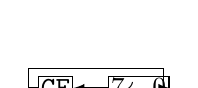
\begin{tikzpicture}[
			framed/.style={ rectangle, draw=black, inner sep=1 },
			arrow/.style={thin,->,-latex}]

			\node[framed] (cf) {\tt CF};
			\node[framed] (bits) at([xshift=3em]cf) {7$\leftarrow$0};
			\IfEqCase{#1} {
				{0}{}
				{}{\node(reg) at([yshift=-1em]bits) {\tt #2};}
			}

			\draw[arrow] (bits) -- (cf);
			\draw[arrow] (cf.west) |- +(-0.12,0) |- +(1.6,0.25) |- (bits.east);
		\end{tikzpicture}
	}
}

\newcommand{\SymRLC}[2][]{
	\SymDrawing{
		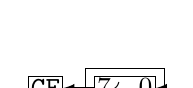
\begin{tikzpicture}[
			framed/.style={rectangle, draw=black, inner sep=1},
			arrow/.style={thin,->,-latex}]
				
			\node[framed] (cf) {\tt CF};
			\node[framed, right=1.1em of cf] (bits) {7$\leftarrow$0};
			\IfEqCase{#1} {
				{0}{}
				{}{\node[below=-1pt of bits](reg) {\tt #2};}
			}
				
			\draw[arrow] (bits) -- (cf);
			\draw[arrow] (bits.west) |- +(-0.1,0) |- +(0.9,0.25) |- (bits.east);
		\end{tikzpicture}
	}
}

\newcommand{\SymRLCu}[3][]{
	\IfEqCase{#1}{
		{0}{#2$\leftarrow$(#3+d)}
		{1}{RLC #2}
		{2}{(#3+d)$\leftarrow$#2}
		{}{\SymRLCu[0]{#2}{#3}\\\SymRLCu[1]{#2}{#3}\\\SymRLCu[2]{#2}{#3}}
	}
}

\newcommand{\SymRLD}{
	\SymDrawing{
		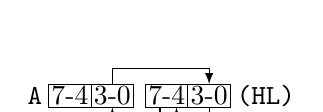
\begin{tikzpicture}[
			framed/.style={rectangle, draw=black, inner sep=1, outer sep=0},
			plain/.style={inner sep=0},
			arrow/.style={thin,->,-latex}]
			
			\node[plain] (a) {\tt A};
			
			\node[framed, right=0.5ex of a] (bitsAhi) {7-4};
			\node[framed, right=0ex of bitsAhi] (bitsAlo) {3-0};

			\node[framed, right=1ex of bitsAlo] (bitsHLhi) {7-4};
			\node[framed, right=0ex of bitsHLhi] (bitsHLlo) {3-0};
 			
			\node[plain, right=0.5ex of bitsHLlo] (hl) {\tt (HL)};
			
			\draw[arrow] (bitsHLlo.south) |- +(-0.2,-0.2) -| (bitsHLhi.310);
			\draw[arrow] (bitsHLhi.240) |- +(-0.2,-0.2) -| (bitsAlo.south);
			\draw[arrow] (bitsAlo.north) |- +(0.2,0.2) -| (bitsHLlo.north);
		\end{tikzpicture}
	}
}

\newcommand{\SymRR}[2][]{
	\SymDrawing{
		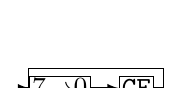
\begin{tikzpicture}[
			framed/.style={ rectangle, draw=black, inner sep=1 },
			arrow/.style={thin,->,-latex}]

			\node[framed] (bits) {7$\rightarrow$0};
			\node[framed, right=1em of bits] (cf) {\tt CF};
			\IfEqCase{#1} {
				{0}{}
				{}{\node[below=-1pt of bits](reg) {\tt #2};}
			}

			\draw[arrow] (bits) -- (cf);
			\draw[arrow] (cf.east) |- +(0.12,0) |- +(-1.6,0.25) |- (bits.west);
		\end{tikzpicture}
	}
}

\newcommand{\SymRRC}[2][]{
	\SymDrawing{
		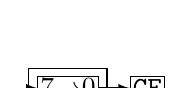
\begin{tikzpicture}[
			framed/.style={rectangle, draw=black, inner sep=1},
			arrow/.style={thin,->,-latex}]
			
			\node[framed] (bits) {7$\rightarrow$0};
			\node[framed, right=1.1em of bits] (cf) {\tt CF};
			\IfEqCase{#1} {
				{0}{}
				{}{\node[below=-1pt of bits](reg) {\tt #2};}
			}
			
			\draw[arrow] (bits) -- (cf);
			\draw[arrow] (bits.east) |- +(0.1,0) |- +(-0.9,0.25) |- (bits.west);
		\end{tikzpicture}
	}
}

\newcommand{\SymRRD}{
	\SymDrawing{
		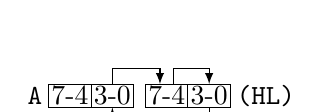
\begin{tikzpicture}[
			framed/.style={rectangle, draw=black, inner sep=1, outer sep=0},
			plain/.style={inner sep=0},
			arrow/.style={thin,->,-latex}]
			
			\node[plain] (a) {\tt A};
			
			\node[framed, right=0.5ex of a] (bitsAhi) {7-4};
			\node[framed, right=0ex of bitsAhi] (bitsAlo) {3-0};

			\node[framed, right=1ex of bitsAlo] (bitsHLhi) {7-4};
			\node[framed, right=0ex of bitsHLhi] (bitsHLlo) {3-0};
 			
			\node[plain, right=0.5ex of bitsHLlo] (hl) {\tt (HL)};
			
			\draw[arrow] (bitsHLlo.south) |- +(-0.2,-0.2) -| (bitsAlo.south);
			\draw[arrow] (bitsAlo.north) |- +(0.2,0.2) -| (bitsHLhi.120);
			\draw[arrow] (bitsHLhi.60) |- +(0.2,0.2) -| (bitsHLlo.north);
		\end{tikzpicture}
	}
}

\newcommand{\SymRST}[2][]{
	\IfEqCase{#1}{
		{0}{(SP-1)$\leftarrow$PC\High}
		{1}{(SP-2)$\leftarrow$PC\Low}
		{2}{SP$\leftarrow$SP-2}
		{3}{PC$\leftarrow$#2}
		{}{\SymRST[0]{#2}\\\SymRST[1]{#2}\\\SymRST[2]{#2}\\\SymRST[3]{#2}}
	}
}

\newcommand{\SymSET}[1]{$\mathtt{#1_b}\leftarrow$1}

\newcommand{\SymSETu}[3][]{
	\IfEqCase{#1}{
		{0}{#2$\leftarrow$(#3+d)}
		{1}{$\mathtt{#2_b}\leftarrow$1}
		{2}{(#3+d)$\leftarrow$#2}
		{}{\SymSETu[0]{#2}{#3}\\\SymSETu[1]{#2}{#3}\\\SymSETu[2]{#2}{#3}}
	}
}

\newcommand{\SymSBC}[2]{#1$\leftarrow$#1-#2-CF}

\newcommand{\SymSCF}{CF$\leftarrow$1}

\newcommand{\SymSETAE}{A$\leftarrow$unsigned(\$80)>>(E$\wedge$7)}

\newcommand{\SymSLA}[2][]{
	\SymDrawing{
		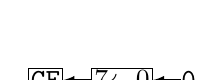
\begin{tikzpicture}[
			framed/.style={rectangle, draw=black, inner sep=1},
			plain/.style={inner sep=0},
			arrow/.style={thin,->,-latex}]

			\node[framed] (cf) {\tt CF};
			\node[framed, right=1em of cf] (bits) {7$\leftarrow$0};
			\node[plain, right=1em of bits] (zero) {\tt 0};
			\IfEqCase{#1} {
				{0}{}
				{}{\node[below=-1pt of bits](reg) {\tt #2};}
			}

			\draw[arrow] (zero) -- (bits);
			\draw[arrow] (bits) -- (cf);
		\end{tikzpicture}
	}
}

\newcommand{\SymSLI}[2][]{
	\SymDrawing{
		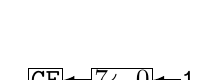
\begin{tikzpicture}[
			framed/.style={rectangle, draw=black, inner sep=1},
			plain/.style={inner sep=0},
			arrow/.style={thin,->,-latex}]

			\node[framed] (cf) {\tt CF};
			\node[framed, right=1em of cf] (bits) {7$\leftarrow$0};
			\node[plain, right=1em of bits] (one) {\tt 1};
			\IfEqCase{#1} {
				{0}{}
				{}{\node[below=-1pt of bits](reg) {\tt #2};}
			}

			\draw[arrow] (one) -- (bits);
			\draw[arrow] (bits) -- (cf);
		\end{tikzpicture}
	}
}

\newcommand{\SymSRA}[2][]{
	\SymDrawing{
		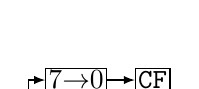
\begin{tikzpicture}[
			framed/.style={rectangle, draw=black, inner sep=1},
			arrow/.style={thin,->,-latex}]
				
			\node[framed] (bits) {7$\rightarrow$0};
			\node[framed, right=1em of bits] (cf) {\tt CF};
			\IfEqCase{#1} {
				{0}{}
				{}{\node[below=-1pt of bits](reg) {\tt #2};}
			}
				
			\draw[arrow] (bits) -- (cf);
			\draw[arrow] (bits.211) |- +(-0.35,-0.1) |- (bits.west);
		\end{tikzpicture}
	}
}

\newcommand{\SymSRL}[2][]{
	\SymDrawing{
		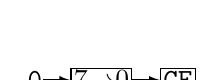
\begin{tikzpicture}[
			framed/.style={rectangle, draw=black, inner sep=1},
			plain/.style={inner sep=0},
			arrow/.style={thin,->,-latex}]
			
			\node[plain] (zero) {\tt 0};
			\node[framed, right=1em of zero] (bits) {7$\rightarrow$0};
			\node[framed, right=1em of bits] (cf) {\tt CF};
			\IfEqCase{#1} {
				{0}{}
				{}{\node[below=-1pt of bits](reg) {\tt #2};}
			}
			
			\draw[arrow] (zero) -- (bits);
			\draw[arrow] (bits) -- (cf);
		\end{tikzpicture}
	}
}

\newcommand{\SymSUB}[1]{A$\leftarrow$A-#1}

\newcommand{\SymSWAPNIB}[1][]{
	\IfEq{#1}{}{}{\hspace*{-1.6em}}
	\SymDrawing{
		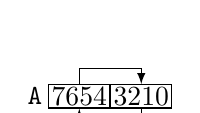
\begin{tikzpicture}[
			framed/.style={rectangle, draw=black, inner sep=1},
			plain/.style={inner sep=0},
			arrow/.style={thin,->,-latex}]
			
			\node[plain] (a) {\tt A};
			\node[framed, right=0.2em of a] (hi) {7654};
			\node[framed, right=0em of hi] (lo) {3210};
			
			\draw[arrow] (hi.north) |- +(0.1,0.2) -| (lo.north);
			\draw[arrow] (lo.south) |- +(-0.1,-0.2) -| (hi.south);
		\end{tikzpicture}
	}
}

\newcommand{\SymTEST}{A$\wedge$n}

\newcommand{\SymXOR}[1]{A$\leftarrow$A$\veebar$#1}

% ────────────────────────────────────────────────────────────────────────────
% ─██████████████─██████─────────██████████████─██████████████─██████████████─
% ─██░░░░░░░░░░██─██░░██─────────██░░░░░░░░░░██─██░░░░░░░░░░██─██░░░░░░░░░░██─
% ─██░░██████████─██░░██─────────██░░██████░░██─██░░██████████─██░░██████████─
% ─██░░██─────────██░░██─────────██░░██──██░░██─██░░██─────────██░░██─────────
% ─██░░██████████─██░░██─────────██░░██████░░██─██░░██─────────██░░██████████─
% ─██░░░░░░░░░░██─██░░██─────────██░░░░░░░░░░██─██░░██──██████─██░░░░░░░░░░██─
% ─██░░██████████─██░░██─────────██░░██████░░██─██░░██──██░░██─██████████░░██─
% ─██░░██─────────██░░██─────────██░░██──██░░██─██░░██──██░░██─────────██░░██─
% ─██░░██─────────██░░██████████─██░░██──██░░██─██░░██████░░██─██████████░░██─
% ─██░░██─────────██░░░░░░░░░░██─██░░██──██░░██─██░░░░░░░░░░██─██░░░░░░░░░░██─
% ─██████─────────██████████████─██████──██████─██████████████─██████████████─
% ────────────────────────────────────────────────────────────────────────────

% some common declarations to unify formatting of individual parts; we can then later redefine these macros to change appearance without having to tweak main macros
\newcommand{\FlagsSee}[1]{\See{#1}}		% footnote declarations
\newcommand{\FlagsFPP}{\FPP}			% PF=parity indicator
\newcommand{\FlagsFPV}{\FPV}			% PF=overflow indicator
\newcommand{\FlagsSmall}[1]{\tiny #1}	% small font size
\newcommand{\FlagsNoEffect}{}			% text for "no effect"; we don't display anything in tables, but may redeclare to display something in details section

% note: because LaTeX doesn't allow numbers in commands, we use the following notation:
% r = 8 bit register or number
% n = 8 bit number (only if we already use r)
% rr = 16 bit register pair or number
% nn = 16 bit number (only if we already use rr)
% note: we need to pass 1 optional parameter to Flags; we need it in details section

% order of the parameters: SF, ZF, HF, PV, NF, CF
\newcommand{\FlagsADDr}[1][]{\Flags[#1]{\FS}{\FS}{\FS}{\FlagsFPV}{0}{\FS}}
\newcommand{\FlagsADDrr}[1][]{\Flags[#1]{\FN}{\FN}{\FS\FlagsSee{2}}{\FN}{0}{\FS\FlagsSee{1}}}
\newcommand{\FlagsADDrra}[1][\FlagsNoEffect]{\Flags[#1]{\FN}{\FN}{\FN}{\FN}{\FN}{\FU\FlagsSee{1}}}
\newcommand{\FlagsADDrrnn}[1][\FlagsNoEffect]{\Flags[#1]{\FN}{\FN}{\FN}{\FN}{\FN}{\FN}}
\newcommand{\FlagsADCr}[1][]{\Flags[#1]{\FS}{\FS}{\FS}{\FlagsFPV}{0}{\FS}}
\newcommand{\FlagsADCrr}[1][]{\Flags[#1]{\FS\FlagsSee{1}}{\FS\FlagsSee{1}}{\FS\FlagsSee{2}}{\FlagsFPV\FlagsSee{1}}{0}{\FS\FlagsSee{1}}}
\newcommand{\FlagsANDr}[1][]{\Flags[#1]{\FS}{\FS}{1}{\FlagsFPP}{0}{0}}
\newcommand{\FlagsBITr}[1][]{\Flags[#1]{\FU\FlagsSee{1}}{\FS}{1}{\FU\FlagsSee{1}}{0}{\FN}}
\newcommand{\FlagsBSLA}[1][\FlagsNoEffect]{\Flags[#1]{\FN}{\FN}{\FN}{\FN}{\FN}{\FN}}
\newcommand{\FlagsBSRA}[1][\FlagsNoEffect]{\Flags[#1]{\FN}{\FN}{\FN}{\FN}{\FN}{\FN}}
\newcommand{\FlagsBSRL}[1][\FlagsNoEffect]{\Flags[#1]{\FN}{\FN}{\FN}{\FN}{\FN}{\FN}}
\newcommand{\FlagsBSRF}[1][\FlagsNoEffect]{\Flags[#1]{\FN}{\FN}{\FN}{\FN}{\FN}{\FN}}
\newcommand{\FlagsBRLC}[1][\FlagsNoEffect]{\Flags[#1]{\FN}{\FN}{\FN}{\FN}{\FN}{\FN}}
\newcommand{\FlagsCALLnn}[1][\FlagsNoEffect]{\Flags[#1]{\FN}{\FN}{\FN}{\FN}{\FN}{\FN}}
\newcommand{\FlagsCALLccnn}[1][\FlagsNoEffect]{\Flags[#1]{\FN}{\FN}{\FN}{\FN}{\FN}{\FN}}
\newcommand{\FlagsCCF}[1][]{\Flags[#1]{\FN}{\FN}{\FN\FlagsSee{2}}{\FN}{0}{\FS}}
\newcommand{\FlagsCPr}[1][]{\Flags[#1]{\FS}{\FS}{\FS}{\FlagsFPV}{1}{\FS}}
\newcommand{\FlagsCPI}[1][]{\Flags[#1]{\FS\FlagsSee{1}}{\FX\FlagsSee{2}}{\FS\FlagsSee{1}}{\FX\FlagsSee{3}}{1}{\FN}}
\newcommand{\FlagsCPIR}[1][]{\Flags[#1]{\FS\FlagsSee{1}}{\FX\FlagsSee{2}}{\FS\FlagsSee{1}}{\FX\FlagsSee{3}}{1}{\FN}}
\newcommand{\FlagsCPD}[1][]{\Flags[#1]{\FS\FlagsSee{1}}{\FX\FlagsSee{2}}{\FS\FlagsSee{1}}{\FX\FlagsSee{3}}{1}{\FN}}
\newcommand{\FlagsCPDR}[1][]{\Flags[#1]{\FS\FlagsSee{1}}{\FX\FlagsSee{2}}{\FS\FlagsSee{1}}{\FX\FlagsSee{3}}{1}{\FN}}
\newcommand{\FlagsCPL}[1][]{\Flags[#1]{\FN}{\FN}{1}{\FN}{1}{\FN}}
\newcommand{\FlagsDAA}[1][]{\Flags[#1]{\FS}{\FS}{\FS}{\FlagsFPP}{\FN}{\FS}}
\newcommand{\FlagsDECr}[1][]{\Flags[#1]{\FS}{\FS}{\FS}{\FlagsFPV\FlagsSee{5}}{1}{\FN}}
\newcommand{\FlagsDECrr}[1][\FlagsNoEffect]{\Flags[#1]{\FN}{\FN}{\FN}{\FN}{\FN}{\FN}}
\newcommand{\FlagsDI}[1][\FlagsNoEffect]{\Flags[#1]{\FN}{\FN}{\FN}{\FN}{\FN}{\FN}}
\newcommand{\FlagsDJNZ}[1][\FlagsNoEffect]{\Flags[#1]{\FN}{\FN}{\FN}{\FN}{\FN}{\FN}}
\newcommand{\FlagsEI}[1][\FlagsNoEffect]{\Flags[#1]{\FN}{\FN}{\FN}{\FN}{\FN}{\FN}}
\newcommand{\FlagsEXrr}[1][\FlagsNoEffect]{\Flags[#1]{\FN}{\FN}{\FN}{\FN}{\FN}{\FN}}
\newcommand{\FlagsEXaf}[1][]{\Flags[#1]{\FX\FlagsSee{1}}{\FX\FlagsSee{1}}{\FX\FlagsSee{1}}{\FX\FlagsSee{1}}{\FX\FlagsSee{1}}{\FX\FlagsSee{1}}}
\newcommand{\FlagsEXX}[1][\FlagsNoEffect]{\Flags[#1]{\FN}{\FN}{\FN}{\FN}{\FN}{\FN}}
\newcommand{\FlagsHALT}[1][\FlagsNoEffect]{\Flags[#1]{\FN}{\FN}{\FN}{\FN}{\FN}{\FN}}
\newcommand{\FlagsIM}[1][\FlagsNoEffect]{\Flags[#1]{\FN}{\FN}{\FN}{\FN}{\FN}{\FN}}
\newcommand{\FlagsINan}[1][\FlagsNoEffect]{\Flags[#1]{\FN}{\FN}{\FN}{\FN}{\FN}{\FN}}
\newcommand{\FlagsINrc}[1][]{\Flags[#1]{\FS}{\FS}{0}{\FlagsFPP}{0}{\FN}}
\newcommand{\FlagsINc}[1][]{\Flags[#1]{\FS}{\FS}{0}{\FlagsFPP}{0}{\FN}}
\newcommand{\FlagsINCr}[1][]{\Flags[#1]{\FS}{\FS}{\FS}{\FlagsFPV\FlagsSee{4}}{0}{\FN}}
\newcommand{\FlagsINCrr}[1][\FlagsNoEffect]{\Flags[#1]{\FN}{\FN}{\FN}{\FN}{\FN}{\FN}}
\newcommand{\FlagsINI}[1][]{\Flags[#1]{\FX\FlagsSee{5}}{\FX\FlagsSee{4}}{\FX\FlagsSee{5}}{\FX\FlagsSee{5}}{1}{\FN}}
\newcommand{\FlagsINIR}[1][]{\Flags[#1]{\FX\FlagsSee{5}}{1}{\FX\FlagsSee{5}}{\FX\FlagsSee{5}}{1}{\FN}}
\newcommand{\FlagsIND}[1][]{\Flags[#1]{\FX\FlagsSee{5}}{\FX\FlagsSee{4}}{\FX\FlagsSee{5}}{\FX\FlagsSee{5}}{1}{\FN}}
\newcommand{\FlagsINDR}[1][]{\Flags[#1]{\FX\FlagsSee{5}}{1}{\FX\FlagsSee{5}}{\FX\FlagsSee{5}}{1}{\FN}}
\newcommand{\FlagsJPc}[1][]{\Flags[#1]{\FU}{\FU}{\FU}{\FU}{\FU}{\FU}}
\newcommand{\FlagsJPnn}[1][\FlagsNoEffect]{\Flags[#1]{\FN}{\FN}{\FN}{\FN}{\FN}{\FN}}
\newcommand{\FlagsJPccnn}[1][\FlagsNoEffect]{\Flags[#1]{\FN}{\FN}{\FN}{\FN}{\FN}{\FN}}
\newcommand{\FlagsJPrr}[1][\FlagsNoEffect]{\Flags[#1]{\FN}{\FN}{\FN}{\FN}{\FN}{\FN}}
\newcommand{\FlagsJRn}[1][\FlagsNoEffect]{\Flags[#1]{\FN}{\FN}{\FN}{\FN}{\FN}{\FN}}
\newcommand{\FlagsJRccn}[1][\FlagsNoEffect]{\Flags[#1]{\FN}{\FN}{\FN}{\FN}{\FN}{\FN}}
\newcommand{\FlagsLDr}[1][\FlagsNoEffect]{\Flags[#1]{\FN}{\FN}{\FN}{\FN}{\FN}{\FN}}
\newcommand{\FlagsLDrr}[1][\FlagsNoEffect]{\Flags[#1]{\FN}{\FN}{\FN}{\FN}{\FN}{\FN}}
\newcommand{\FlagsLDair}[1][]{\Flags[#1]{\FS}{\FS}{0}{{\FlagsSmall IFF2}}{0}{\FN}}
\newcommand{\FlagsLDI}[1][]{\Flags[#1]{\FN}{\FN}{0}{\FX\FlagsSee{3}}{0}{\FN}}
\newcommand{\FlagsLDIR}[1][]{\Flags[#1]{\FN}{\FN}{0}{0\FlagsSee{4}}{0}{\FN}}
\newcommand{\FlagsLDD}[1][]{\Flags[#1]{\FN}{\FN}{0}{\FX\FlagsSee{3}}{0}{\FN}}
\newcommand{\FlagsLDDR}[1][]{\Flags[#1]{\FN}{\FN}{0}{0\FlagsSee{4}}{0}{\FN}}
\newcommand{\FlagsLDDX}[1][\FlagsNoEffect]{\Flags[#1]{\FN}{\FN}{\FN}{\FN}{\FN}{\FN}}
\newcommand{\FlagsLDDRX}[1][\FlagsNoEffect]{\Flags[#1]{\FN}{\FN}{\FN}{\FN}{\FN}{\FN}}
\newcommand{\FlagsLDIX}[1][\FlagsNoEffect]{\Flags[#1]{\FN}{\FN}{\FN}{\FN}{\FN}{\FN}}
\newcommand{\FlagsLDIRX}[1][\FlagsNoEffect]{\Flags[#1]{\FN}{\FN}{\FN}{\FN}{\FN}{\FN}}
\newcommand{\FlagsLDPIRX}[1][\FlagsNoEffect]{\Flags[#1]{\FN}{\FN}{\FN}{\FN}{\FN}{\FN}}
\newcommand{\FlagsLDWS}[1][]{\Flags[#1]{\FS}{\FS}{\FS}{\FlagsFPV\FlagsSee{3}}{0}{\FN}}
\newcommand{\FlagsMIRRORa}[1][\FlagsNoEffect]{\Flags[#1]{\FN}{\FN}{\FN}{\FN}{\FN}{\FN}}
\newcommand{\FlagsMULde}[1][\FlagsNoEffect]{\Flags[#1]{\FN}{\FN}{\FN}{\FN}{\FN}{\FN}}
\newcommand{\FlagsNEG}[1][]{\Flags[#1]{\FS}{\FS}{\FS}{\FlagsFPP}{1}{\FS}}
\newcommand{\FlagsNEXTREGna}[1][\FlagsNoEffect]{\Flags[#1]{\FN}{\FN}{\FN}{\FN}{\FN}{\FN}}
\newcommand{\FlagsNEXTREGnn}[1][\FlagsNoEffect]{\Flags[#1]{\FN}{\FN}{\FN}{\FN}{\FN}{\FN}}
\newcommand{\FlagsNOP}[1][\FlagsNoEffect]{\Flags[#1]{\FN}{\FN}{\FN}{\FN}{\FN}{\FN}}
\newcommand{\FlagsORr}[1][]{\Flags[#1]{\FS}{\FS}{0}{\FlagsFPP}{0}{0}}
\newcommand{\FlagsOUTna}[1][\FlagsNoEffect]{\Flags[#1]{\FN}{\FN}{\FN}{\FN}{\FN}{\FN}}
\newcommand{\FlagsOUTcr}[1][\FlagsNoEffect]{\Flags[#1]{\FN}{\FN}{\FN}{\FN}{\FN}{\FN}}
\newcommand{\FlagsOUTc}[1][\FlagsNoEffect]{\Flags[#1]{\FN}{\FN}{\FN}{\FN}{\FN}{\FN}}
\newcommand{\FlagsOUTI}[1][]{\Flags[#1]{\FX\FlagsSee{2}}{\FX\FlagsSee{1}}{\FX\FlagsSee{2}}{\FX\FlagsSee{2}}{1}{\FN}}
\newcommand{\FlagsOTIR}[1][]{\Flags[#1]{\FX\FlagsSee{2}}{1}{\FX\FlagsSee{2}}{\FX\FlagsSee{2}}{1}{\FN}}
\newcommand{\FlagsOUTD}[1][]{\Flags[#1]{\FX\FlagsSee{2}}{\FX\FlagsSee{1}}{\FX\FlagsSee{2}}{\FX\FlagsSee{2}}{1}{\FN}}
\newcommand{\FlagsOTDR}[1][]{\Flags[#1]{\FX\FlagsSee{2}}{1}{\FX\FlagsSee{2}}{\FX\FlagsSee{2}}{1}{\FN}}
\newcommand{\FlagsOUTINB}[1][]{\Flags[#1]{\FU}{\FU}{\FU}{\FU}{\FU}{\FU}}
\newcommand{\FlagsPIXELAD}[1][\FlagsNoEffect]{\Flags[#1]{\FN}{\FN}{\FN}{\FN}{\FN}{\FN}}
\newcommand{\FlagsPIXELDN}[1][\FlagsNoEffect]{\Flags[#1]{\FN}{\FN}{\FN}{\FN}{\FN}{\FN}}
\newcommand{\FlagsPOPrr}[1][\FlagsNoEffect]{\Flags[#1]{\FN}{\FN}{\FN}{\FN}{\FN}{\FN}}
\newcommand{\FlagsPOPaf}[1][]{\Flags[#1]{\FS\FlagsSee{1}}{\FS\FlagsSee{1}}{\FS\FlagsSee{1}}{\FS\FlagsSee{1}}{\FS\FlagsSee{1}}{\FS\FlagsSee{1}}}
\newcommand{\FlagsPUSHrr}[1][\FlagsNoEffect]{\Flags[#1]{\FN}{\FN}{\FN}{\FN}{\FN}{\FN}}
\newcommand{\FlagsPUSHnn}[1][\FlagsNoEffect]{\Flags[#1]{\FN}{\FN}{\FN}{\FN}{\FN}{\FN}}
\newcommand{\FlagsRESr}[1][\FlagsNoEffect]{\Flags[#1]{\FN}{\FN}{\FN}{\FN}{\FN}{\FN}}
\newcommand{\FlagsRET}[1][\FlagsNoEffect]{\Flags[#1]{\FN}{\FN}{\FN}{\FN}{\FN}{\FN}}
\newcommand{\FlagsRETcc}[1][\FlagsNoEffect]{\Flags[#1]{\FN}{\FN}{\FN}{\FN}{\FN}{\FN}}
\newcommand{\FlagsRETI}[1][\FlagsNoEffect]{\Flags[#1]{\FN}{\FN}{\FN}{\FN}{\FN}{\FN}}
\newcommand{\FlagsRETN}[1][\FlagsNoEffect]{\Flags[#1]{\FN}{\FN}{\FN}{\FN}{\FN}{\FN}}
\newcommand{\FlagsRLr}[1][]{\Flags[#1]{\FS}{\FS}{0}{\FlagsFPP}{0}{\FS}}
\newcommand{\FlagsRLA}[1][]{\Flags[#1]{\FN}{\FN}{0}{\FN}{0}{\FS}}
\newcommand{\FlagsRLCr}[1][]{\Flags[#1]{\FS}{\FS}{0}{\FlagsFPP}{0}{\FS}}
\newcommand{\FlagsRLCA}[1][]{\Flags[#1]{\FN}{\FN}{0}{\FN}{0}{\FS}}
\newcommand{\FlagsRLD}[1][]{\Flags[#1]{\FS}{\FS}{0}{\FlagsFPP}{0}{\FN}}
\newcommand{\FlagsRRr}[1][]{\Flags[#1]{\FS}{\FS}{0}{\FlagsFPP}{0}{\FS}}
\newcommand{\FlagsRRA}[1][]{\Flags[#1]{\FN}{\FN}{0}{\FN}{0}{\FS}}
\newcommand{\FlagsRRCr}[1][]{\Flags[#1]{\FS}{\FS}{0}{\FlagsFPP}{0}{\FS}}
\newcommand{\FlagsRRCA}[1][]{\Flags[#1]{\FN}{\FN}{0}{\FN}{0}{\FS}}
\newcommand{\FlagsRRD}[1][]{\Flags[#1]{\FS}{\FS}{0}{\FlagsFPP}{0}{\FN}}
\newcommand{\FlagsRSTn}[1][\FlagsNoEffect]{\Flags[#1]{\FN}{\FN}{\FN}{\FN}{\FN}{\FN}}
\newcommand{\FlagsSBCr}[1][]{\Flags[#1]{\FS}{\FS}{\FS}{\FlagsFPV}{1}{\FS}}
\newcommand{\FlagsSBCrr}[1][]{\Flags[#1]{\FS\FlagsSee{1}}{\FS\FlagsSee{1}}{\FS\FlagsSee{2}}{\FlagsFPV\FlagsSee{1}}{1}{\FS\FlagsSee{1}}}
\newcommand{\FlagsSCF}[1][]{\Flags[#1]{\FN}{\FN}{0}{\FN}{0}{1}}
\newcommand{\FlagsSETr}[1][\FlagsNoEffect]{\Flags[#1]{\FN}{\FN}{\FN}{\FN}{\FN}{\FN}}
\newcommand{\FlagsSETAE}[1][\FlagsNoEffect]{\Flags[#1]{\FN}{\FN}{\FN}{\FN}{\FN}{\FN}}
\newcommand{\FlagsSLAr}[1][]{\Flags[#1]{\FS}{\FS}{0}{\FlagsFPP}{0}{\FS}}
\newcommand{\FlagsSLIr}[1][]{\Flags[#1]{\FS}{\FS}{0}{\FlagsFPP}{0}{\FS}}
\newcommand{\FlagsSRAr}[1][]{\Flags[#1]{\FS}{\FS}{0}{\FlagsFPP}{0}{\FS}}
\newcommand{\FlagsSRLr}[1][]{\Flags[#1]{\FS}{\FS}{0}{\FlagsFPP}{0}{\FS}}
\newcommand{\FlagsSUBr}[1][]{\Flags[#1]{\FS}{\FS}{\FS}{\FlagsFPV}{1}{\FS}}
\newcommand{\FlagsSWAPNIB}[1][\FlagsNoEffect]{\Flags[#1]{\FN}{\FN}{\FN}{\FN}{\FN}{\FN}}
\newcommand{\FlagsTESTn}[1][]{\Flags[#1]{\FS}{\FS}{\FS}{\FlagsFPP}{\FU}{\FS}}
\newcommand{\FlagsXORr}[1][]{\Flags[#1]{\FS}{\FS}{0}{\FlagsFPP}{0}{0}}



% ASCII text created with https://fsymbols.com/generators/carty/
% in case it's not obvious - these large titles are nicely visible in minimap¯\_(ツ)_/¯

\begin{document}

	% note: each section must be `\include{}`ed; LaTeX will do a `\clearpage` in front which is what is desired. However if we just want to split larger section into multiple files, `\input{}` should be used instead which imports the contents of the file as if they were typed here.
	% important: regardles of whether `\include{}` or `\input{}` is used, `.tex` extension must be ommited. Some LaTeX compilers auto-add the extension so it ends up doubled (`*.tex.tex`) and therefore file cannot be found. Works with MikTEX either way.

	% ▒█▀▀▀ ▒█▀▀█ ▒█▀▀▀█ ▒█▄░▒█ ▀▀█▀▀ 
	% ▒█▀▀▀ ▒█▄▄▀ ▒█░░▒█ ▒█▒█▒█ ░▒█░░ 
	% ▒█░░░ ▒█░▒█ ▒█▄▄▄█ ▒█░░▀█ ░▒█░░

	\SetupPageFormattingTitle

	% ████████████████████████████████████████████████████████████████████████
% █░░░░░░░░░░░░░░█░░░░░░░░░░█░░░░░░░░░░░░░░█░░░░░░█████████░░░░░░░░░░░░░░█
% █░░▄▀▄▀▄▀▄▀▄▀░░█░░▄▀▄▀▄▀░░█░░▄▀▄▀▄▀▄▀▄▀░░█░░▄▀░░█████████░░▄▀▄▀▄▀▄▀▄▀░░█
% █░░░░░░▄▀░░░░░░█░░░░▄▀░░░░█░░░░░░▄▀░░░░░░█░░▄▀░░█████████░░▄▀░░░░░░░░░░█
% █████░░▄▀░░███████░░▄▀░░███████░░▄▀░░█████░░▄▀░░█████████░░▄▀░░█████████
% █████░░▄▀░░███████░░▄▀░░███████░░▄▀░░█████░░▄▀░░█████████░░▄▀░░░░░░░░░░█
% █████░░▄▀░░███████░░▄▀░░███████░░▄▀░░█████░░▄▀░░█████████░░▄▀▄▀▄▀▄▀▄▀░░█
% █████░░▄▀░░███████░░▄▀░░███████░░▄▀░░█████░░▄▀░░█████████░░▄▀░░░░░░░░░░█
% █████░░▄▀░░███████░░▄▀░░███████░░▄▀░░█████░░▄▀░░█████████░░▄▀░░█████████
% █████░░▄▀░░█████░░░░▄▀░░░░█████░░▄▀░░█████░░▄▀░░░░░░░░░░█░░▄▀░░░░░░░░░░█
% █████░░▄▀░░█████░░▄▀▄▀▄▀░░█████░░▄▀░░█████░░▄▀▄▀▄▀▄▀▄▀░░█░░▄▀▄▀▄▀▄▀▄▀░░█
% █████░░░░░░█████░░░░░░░░░░█████░░░░░░█████░░░░░░░░░░░░░░█░░░░░░░░░░░░░░█
% ████████████████████████████████████████████████████████████████████████

\title{\BookTitle}
\author{\AuthorNameSurname}
\date{\LatestRevisionName}


\begin{titlepage}
	\newcommand{\BigFont}[1]{\fontsize{30}{30}\selectfont #1}
	\newcommand{\MidFont}[1]{\fontsize{21.4}{21}\selectfont #1}
	\newcommand{\SmallFont}[1]{\fontsize{14}{14}\selectfont #1}
	\newcommand{\MiniFont}[1]{\fontsize{8}{8}\selectfont #1}
	
	\WorkInProgressFullScreen

	\vspace*{\fill}

	\begin{flushright}
		\sffamily

		\textbf{
			\BigFont{\BookTitleMain}
			\\[0.5cm]
			\MidFont{\BookTitleSub\hspace*{-0.8ex}}
			% ^^^ for some reason there's some horizontal space at the right side of subtitle instead of being nicely aligned with the rest of the text... \hspace takes care of that
		}

		\vspace*{2cm}

		\MidFont{\AuthorNameSurname}

		\vspace*{5cm}

		\SmallFont{Z80 Undocumented by}\\
		\SmallFont{Jan Wilmans}\\
		\SmallFont{Sean Young}

	\end{flushright}

	\vspace*{\fill}

	\WorkInProgressFullScreen
	
\end{titlepage}


	\SetupPageFormattingIntro
	
	\begingroup
	{\WorkInProgressFullScreen}

	\vspace*{\fill} % render at the bottom of the page

	{\Large\textbf{\BookTitle}}

	\vspace*{0.1cm}

	{\large\AuthorNameSurname}

	\LatestRevisionName

	REVISIONS\\
	\LatestRevisionDate\\
	2022-11-11\\
	2021-07-16

	\vspace*{0.2cm}

	Copyright {\copyright} \LatestYear ~\AuthorNameSurname\\	% note this should become 2021-\LatestYear (aka 2021-2022) for releases after 2021...
	Copyright {\copyright} 2005 Jan Wilmans\\
	Copyright {\copyright} 1997, 1998, 2001, 2003, 2005 Sean Young

	Permission is granted to copy, distribute and/or modify this document under the terms of the GNU Free Documentation License, Version 1.1 or any later version published by the Free Software Foundation; with no Invariant Sections, with no Front-Cover Texts, and with no Back-Cover Texts. A copy of the license is included in the section entitled ``GNU Free Documentation License''.
\endgroup

	\include{chapter-acknowledge}

	\SetupPageFormattingTOC

	% ██████████████████████████████████████████████
% █░░░░░░░░░░░░░░█░░░░░░░░░░░░░░█░░░░░░░░░░░░░░█
% █░░▄▀▄▀▄▀▄▀▄▀░░█░░▄▀▄▀▄▀▄▀▄▀░░█░░▄▀▄▀▄▀▄▀▄▀░░█
% █░░░░░░▄▀░░░░░░█░░▄▀░░░░░░▄▀░░█░░▄▀░░░░░░░░░░█
% █████░░▄▀░░█████░░▄▀░░██░░▄▀░░█░░▄▀░░█████████
% █████░░▄▀░░█████░░▄▀░░██░░▄▀░░█░░▄▀░░█████████
% █████░░▄▀░░█████░░▄▀░░██░░▄▀░░█░░▄▀░░█████████
% █████░░▄▀░░█████░░▄▀░░██░░▄▀░░█░░▄▀░░█████████
% █████░░▄▀░░█████░░▄▀░░██░░▄▀░░█░░▄▀░░█████████
% █████░░▄▀░░█████░░▄▀░░░░░░▄▀░░█░░▄▀░░░░░░░░░░█
% █████░░▄▀░░█████░░▄▀▄▀▄▀▄▀▄▀░░█░░▄▀▄▀▄▀▄▀▄▀░░█
% █████░░░░░░█████░░░░░░░░░░░░░░█░░░░░░░░░░░░░░█
% ██████████████████████████████████████████████


\tableofcontents

% Manually break the page before introduction in non-print version. Non-print PDF TOC includes sub-sub-sections as well therefore spreads much more pages and, more crutially, ends on odd page so introduction chapter that follows would begin on even one.
% Note: when new sub/sections are added in the future that cause TOC to spread onto even page, this whole \ifdefined can be deleted (or commented out to leave it for the future). There's probably automated way to ensure chapters always start on odd page, but nothing I tried worked (I think part of the problem lies in the fact that odd/even is reversed in this document due to how lulu expects PDF to be formatted)
% right now, we don't need the empty page
% \ifdefined\isPDF
% 	\pagebreak
% 	\IntentionallyEmpty
% 	\pagebreak
% \fi


	% ▒█▀▀█ ▒█▀▀▀█ ▒█▄░▒█ ▀▀█▀▀ ▒█▀▀▀ ▒█▄░▒█ ▀▀█▀▀ 
	% ▒█░░░ ▒█░░▒█ ▒█▒█▒█ ░▒█░░ ▒█▀▀▀ ▒█▒█▒█ ░▒█░░ 
	% ▒█▄▄█ ▒█▄▄▄█ ▒█░░▀█ ░▒█░░ ▒█▄▄▄ ▒█░░▀█ ░▒█░░

	\SetupPageFormattingBook

	\chapter{Introduction}

% ████████████████████████████████████████████████████████████████████████████████████
% █░░░░░░░░░░█░░░░░░██████████░░░░░░█░░░░░░░░░░░░░░█░░░░░░░░░░░░░░░░███░░░░░░░░░░░░░░█
% █░░▄▀▄▀▄▀░░█░░▄▀░░░░░░░░░░██░░▄▀░░█░░▄▀▄▀▄▀▄▀▄▀░░█░░▄▀▄▀▄▀▄▀▄▀▄▀░░███░░▄▀▄▀▄▀▄▀▄▀░░█
% █░░░░▄▀░░░░█░░▄▀▄▀▄▀▄▀▄▀░░██░░▄▀░░█░░░░░░▄▀░░░░░░█░░▄▀░░░░░░░░▄▀░░███░░▄▀░░░░░░▄▀░░█
% ███░░▄▀░░███░░▄▀░░░░░░▄▀░░██░░▄▀░░█████░░▄▀░░█████░░▄▀░░████░░▄▀░░███░░▄▀░░██░░▄▀░░█
% ███░░▄▀░░███░░▄▀░░██░░▄▀░░██░░▄▀░░█████░░▄▀░░█████░░▄▀░░░░░░░░▄▀░░███░░▄▀░░██░░▄▀░░█
% ███░░▄▀░░███░░▄▀░░██░░▄▀░░██░░▄▀░░█████░░▄▀░░█████░░▄▀▄▀▄▀▄▀▄▀▄▀░░███░░▄▀░░██░░▄▀░░█
% ███░░▄▀░░███░░▄▀░░██░░▄▀░░██░░▄▀░░█████░░▄▀░░█████░░▄▀░░░░░░▄▀░░░░███░░▄▀░░██░░▄▀░░█
% ███░░▄▀░░███░░▄▀░░██░░▄▀░░░░░░▄▀░░█████░░▄▀░░█████░░▄▀░░██░░▄▀░░█████░░▄▀░░██░░▄▀░░█
% █░░░░▄▀░░░░█░░▄▀░░██░░▄▀▄▀▄▀▄▀▄▀░░█████░░▄▀░░█████░░▄▀░░██░░▄▀░░░░░░█░░▄▀░░░░░░▄▀░░█
% █░░▄▀▄▀▄▀░░█░░▄▀░░██░░░░░░░░░░▄▀░░█████░░▄▀░░█████░░▄▀░░██░░▄▀▄▀▄▀░░█░░▄▀▄▀▄▀▄▀▄▀░░█
% █░░░░░░░░░░█░░░░░░██████████░░░░░░█████░░░░░░█████░░░░░░██░░░░░░░░░░█░░░░░░░░░░░░░░█
% ████████████████████████████████████████████████████████████████████████████████████

\ChapterTOC[]	% don't apply default style for introduction (we want to keep using the simple style without headers)


\section{Where to get this document}

\BookTitle ~is available as coil bound printed book on

\url{https://bit.ly/zx-next-assembly-dev-guide}

You can also download it as PDF document from GitHub where you can also find its source \LaTeX ~form so you can edit it to your preference

\url{https://github.com/tomaz/zx-next-dev-guide}


\section{Companion Source Code}

GitHub repository also includes companion source code. Sample projects were created in a cross-platform environment on Windows so instructions on the following page are written with these in mind. All programs mentioned are available on Linux and macOS; you should be able to run everything on those platforms too, but likely with some deviations. Regardless, these are merely suggestions, you should be able to use your preferred editor or tools.


\pagebreak % we want list of all tools and software to be on the same page
\begin{description}[style=unboxed,leftmargin=0cm]
	\item[Visual Studio Code (\url{https://code.visualstudio.com/})]\hfill
	
	My code editor of choice! I use it with the following plugins:

	\begin{description}[topsep=1pt,labelindent=2em,leftmargin=2em]
		\item[DeZog plugin (\url{https://github.com/maziac/DeZog})]\hfill
	
		Essential plugin; features list is too large to even attempt to enumerate here but essentially turns VS Code into a fully-fledged debugging environment.

		\item[Z80 Macro-Assembler (\url{https://github.com/mborik/z80-macroasm-vscode})]\hfill
		
		Another must-have plugin for the Z80 assembly developer; syntax highlighting, code formatting and code completion, renaming etc.

		\item[Z80 Instruction Set (\url{https://github.com/maziac/z80-instruction-set})]\hfill
		
		Adds mouse hover action above any Z80N instruction for quick info.

		\item[Z80 Assembly meter (\url{https://github.com/theNestruo/z80-asm-meter-vscode})]\hfill
		
		Shows the sum of clock cycles and machine code bytes for all instructions in the current selection.
	\end{description}
	
	\item[sjasmplus 1.18.2 (\url{https://github.com/z00m128/sjasmplus})]\hfill

	Source code includes sjasmplus specific directives for creating {\tt nex} files at the top and bottom of {\tt main.asm} files; if you use a different compiler, you may need to tweak or comment them out.

	VS Code projects are set up to expect binaries in a specific folder. You will need to download and copy so that {\tt sjasmplus.exe} is located in {\tt Tools/sjasmplus}.

	\item[CSpect 2.13.0 (\url{http://cspect.org})]\hfill

	Similar to sjasmplus, CSpect binaries are expected in a specific folder. To install, download and copy so that {\tt CSpect.exe} is located in {\tt Tools/CSpect} folder.

	\item[CSpect Next Image (\url{http://www.zxspectrumnext.online/\#sd})]\hfill

	You will also need to download the ZX Spectrum Next image file and copy it to the folder where {\tt CSpect.exe} is located. I use a 2GB image, hence VS Code project file is configured for that. If you use a different image, make sure to update {\tt .vscode/tasks.json} file.
	
	\item[DeZog CSpect plugin (\url{https://github.com/maziac/DeZogPlugin})]\hfill

	DeZog requires this plugin to be installed to work with CSpect. To install, download and copy to the same folder where {\tt CSpect.exe} is located. Make sure the plugin version matches the DeZog version!

\end{description}

{
	\footnotesize

	\begin{description}[topsep=1pt,itemsep=1pt,labelindent=0pt,leftmargin=0pt]		
		\item[Note:] you need to have CSpect launched before you can run the samples. I created couple tasks\footnotemark~for it: open VS Code command palette ({\tt Ctrl+Shift+P} shortcut on my installation) and select \textit{Tasks: Run Task} option, then select \textit{Launch CSpect} from list. This is only needed once. Afterwards, use \textit{Run \textgreater ~Start Debugging} from the main menu to compile and launch the program.

		\item[Note:] default DeZog port of 11000 doesn't work on my computer, so I changed it to 13000. This needs to be managed in 2 places: {\tt .vscode/launch.json} and on the plugin side. Companion code repository already includes the setup needed, including {\tt DeZogPlugin.dll.config} file, so it should work out of the box.
	
		\item[Note:] sample projects are ready for ZEsarUX as well, select the option from debugging panel in VS Code.
	\end{description}
}

\footnotetext{
	Workspace tasks seem to not be supported in some later VS Code versions. If this is the case for you, copy them to user tasks (shared between projects): open {\tt .vscode/tasks.json} file from any of the sample projects, scroll down a little and copy {\tt Launch CSpect} and {\tt Launch ZEsarUX} tasks to user tasks. You can do this all from within VS Code. To open the user tasks file, open the command palette and start typing {\tt open user tasks}, then select the option from the drop-down menu.
}


\pagebreak % we want next section to be on its own page, fully visible when listing physical book
\section{Background, Contact \& Feedback}

My first computer was ZX Spectrum 48K. Initially, it was only used to play games, but my creative mind soon set me on the path of building simple games of my own in BASIC. While too young to master assembler at that point, the idea stayed with me. ZX Spectrum Next revived my wish to learn Z80 and return to writing games for the platform.
    
My original intent was to have coil bound list of all ZX Next instructions so I can quickly compare. However, after finding Z80 Undocumented online, it felt like a perfect starting point. And with additional information included, it also encouraged me to extend the mere instructions list with the Next specific chapters. In a way, this book represents my notes as I was learning those topics. That being said, I did my best to present information as a reference to keep the book relevant.

During the process, I wanted to tweak or unify the look of various elements. For example instruction tables. Original \LaTeX ~code required applying changes to each and every instance. As \LaTeX ~is all but a programming language, I extracted individual elements into reusable commands which allowed me to tweak appearance in a single place and apply it to the whole document. I also converted almost all drawings from {\tt picture} to {\tt tikz} as it's far more adaptable. With this, I almost completely restructured the original \LaTeX ~code. While this took a lot of time and effort, it allowed me to quickly iterate later on. I really love this aspect of \LaTeX!

English is not my native tongue. And our mind is not the best tool to correct our own work either. Since I can't afford a professional proofreader, mistakes are a matter of fact I'm afraid. If you spot something or want to contribute, feel free to open an issue on GitHub. Pull requests are also welcome! If you want to contribute, but are unsure of what, check the accompanying readme file on GitHub for ideas. If you want to discuss in advance, or for anything else, you can find me on email \email{tkragelj}{gmail}{com} or Twitter {\tt @tomsbarks}.

That being said, I hope you'll enjoy reading this document as much as I did writing it!

Sincerely, \AuthorName


\pagebreak
\section{Z80 Undocumented}

As the saying ``standing on the shoulders of giants'' goes, this book is also based on pre-existing work from Jan and Sean. While my work is ZX Spectrum Next developer-oriented, their original project was more focused on hardware perspective, for Z80 emulator developers.

If interested, you can find it at \url{http://www.myquest.nl/z80undocumented/}.

\begin{description}[style=unboxed,leftmargin=0cm]
	\item[Jan]\hfill
	
	\url{http://www.myquest.nl/z80undocumented/}\\
	Email \email{jw}{dds}{nl}\\
	Twitter \twitter{janwilmans}

	Interested in emulation for a long time, but a few years after Sean started writing this document, I have also started writing my own MSX emulator in 2003 and I've used this document quite a lot. Now (2005) the Z80 emulation is nearing perfection, I decided to add what extra I have learned and comments various people have sent to Sean, to this document.

	I have restyled the document (although very little) to fit my personal needs and I have checked a lot of things that were already in here.
 
	\item[Sean]\hfill

	\url{http://www.msxnet.org/}
	
	Ever since I first started working on an MSX emulator, I've been very interested in getting the emulation absolutely correct - including the undocumented features. Not just to make sure that all games work, but also to make sure that if a program crashes, it crashes exactly the same way if running on an emulator as on the real thing. Only then is perfection achieved.

	I set about collecting information. I found pieces of information on the Internet, but not everything there is to know. So I tried to fill in the gaps, the results of which I put on my website. Various people have helped since then; this is the result of all those efforts and to my knowledge, this document is the most complete.
\end{description}


\pagebreak
\section{ChangeLog}

\begin{description}

	% when adding versions:
	% 1. replace `\LatestRevisionName` with value from macro definition in `defines.tex`
	% 2. update `\LatestRevisionName` with new value in `defines.tex`
	% 3. create new entry here using now updated values (copy item definition from previous version)

	\item[\LatestRevisionName]
	Corrections and updates based on community comments - with special thanks to Peter Ped Helcmanovsky and Alvin Albrecht. Restructured and updated many ZX Next chapters: added sample code to ports, completely restructured memory map and paging, added new palette chapter including 9-bit palette handling, updated ULA with shadow screen info and added Next extended keyboard, DMA, Copper and Hardware IM2 sections. Other than some cosmetic changes: redesigned title, copyright pages etc. Also, many behind the scenes improvements like splitting previous huge single \LaTeX~ file into multiple per-chapter/section. This is not only more manageable but can also compile much faster.

	\item[16 July 2021]
	Added ZX Spectrum Next information and instructions and restructured text for better maintainability and readability.

	\item[18 September 2005]
	Corrected a textual typo in the R register and memory refresh section, thanks to David Aubespin. Corrected the contradiction in the {\tt DAA} section saying the {\tt NF} flag was both affected and unchanged :) thanks to Dan Meir. Added an error in official documentation about the way Interrupt Mode 2 works, thanks to Aaldert Dekker.
	
	\item[15 June 2005]
	Corrected improper notation of {\tt JP x,nn} mnemonics in opcode list, thanks to Laurens Holst. Corrected a mistake in the {\tt INI}, {\tt INIR}, {\tt IND}, {\tt INDR} section and documented a mistake in official Z80 documentation concerning Interrupt Mode 2, thanks to Boris Donko. Thanks to Aaldert Dekker for his ideas, for verifying many assumptions and for writing instruction exercisers for various instruction groups.

	\item[18 May 2005]
	Added an alphabetical list of instructions for easy reference and corrected an error in the 16-bit arithmetic section, {\tt SBC HL,nn} sets the NF flag just like other subtraction instructions, thanks to Fredrik Olssen for pointing that out.

	\item[4 April 2005]
	I (Jan \email{jw}{dds}{nl}) will be maintaining this document from this version on. I restyled the document to fix the page numbering issues, corrected an error in the I/O Block Instructions section, added graphics for the {\tt RLD} and {\tt RRD} instructions and corrected the spelling in several places.

	\item[20 November 2003]
	Again, thanks to Ramsoft, added PV flag to {\tt OUTI}, {\tt INI} and friends. Minor fix to {\tt DAA} tables, other minor fixes.

	\item[13 November 2003]
	Thanks to Ramsoft, add the correct tables for the {\tt DAA} instruction (section \XRef{z80_undocumented_instruction_daa}). Minor corrections \& typos, thanks to Jim Battle, David Sutherland and most of all Fred Limouzin.

	\item[September 2001]
	Previous documents I had written were in plain text and Microsoft Word, which I now find very embarrassing, so I decided to combine them all and use {\LaTeX}. Apart from a full re-write, the only changed information is ``Power on defaults'' (section \XRef{z80_power_on_defaults}) and the algorithm for the CF and HF flags for {\tt OTIR} and friends (section \XRef{z80_undocumented_instructions_io_block}).

\end{description}


\pagebreak
\IntentionallyEmpty
\pagebreak


	\chapter{Zilog Z80}

% ██████████████████████████████████████████████████
% █░░░░░░░░░░░░░░░░░░█░░░░░░░░░░░░░░█░░░░░░░░░░░░░░█
% █░░▄▀▄▀▄▀▄▀▄▀▄▀▄▀░░█░░▄▀▄▀▄▀▄▀▄▀░░█░░▄▀▄▀▄▀▄▀▄▀░░█
% █░░░░░░░░░░░░▄▀▄▀░░█░░▄▀░░░░░░▄▀░░█░░▄▀░░░░░░▄▀░░█
% █████████░░░░▄▀░░░░█░░▄▀░░██░░▄▀░░█░░▄▀░░██░░▄▀░░█
% ███████░░░░▄▀░░░░███░░▄▀░░░░░░▄▀░░█░░▄▀░░██░░▄▀░░█
% █████░░░░▄▀░░░░█████░░▄▀▄▀▄▀▄▀▄▀░░█░░▄▀░░██░░▄▀░░█
% ███░░░░▄▀░░░░███████░░▄▀░░░░░░▄▀░░█░░▄▀░░██░░▄▀░░█
% █░░░░▄▀░░░░█████████░░▄▀░░██░░▄▀░░█░░▄▀░░██░░▄▀░░█
% █░░▄▀▄▀░░░░░░░░░░░░█░░▄▀░░░░░░▄▀░░█░░▄▀░░░░░░▄▀░░█
% █░░▄▀▄▀▄▀▄▀▄▀▄▀▄▀░░█░░▄▀▄▀▄▀▄▀▄▀░░█░░▄▀▄▀▄▀▄▀▄▀░░█
% █░░░░░░░░░░░░░░░░░░█░░░░░░░░░░░░░░█░░░░░░░░░░░░░░█
% ██████████████████████████████████████████████████

% TODO
% - Describe BIT A,(HL) undocumented flags from internal MEMPRT/WZ register
% - Add testing code to appendices

\ChapterTOC

% renders two column instruction table; parameters:
% (optional) first column type; defaults to "l"
% (optional) width ratio of the first column; defaults to 0.3
% (required) first column
% (required) second column
% use \TwoColumnInstr to render individual instruction
\NewDocumentCommand{\TwoColumnInstructions}{ O{l} O{0.3} m m }{
	{
		\tt 
		\vspace*{1em} % we need some spacing above tables

		\begin{parcolumns}[colwidths={1=#2\linewidth}]{2}
			\colchunk{
				\hspace*{0.25cm} % we want to inset left table inwards
				\begin{tabularx}{\linewidth}{#1X}
					#3
				\end{tabularx}
			}
			\colchunk{
				\begin{tabularx}{\linewidth}{#1X}
					#4
				\end{tabularx}
			}
		\end{parcolumns}
	}
}

% renders a title inside two column instruction; parameters:
% (required) the title
\newcommand{\TwoColumnTitle}[1]{
	\multicolumn{2}{l}{\rm #1} \\
}

% renders single instruction spanning accross whole width; parameters:
% (required) the instruction to render
\newcommand{\TwoColumnSingleInstr}[1]{
	\multicolumn{2}{l}{#1} \\
}

% renders individual two column instruction; parameters:
% (required) address
% (required) instruction
\newcommand{\TwoColumnInstr}[2]{
	#1 & #2 \\
}

\pagebreak
\section{Overview}
\subsection{History of the Z80}

In 1969 Intel was approached by a Japanese company called Busicom to produce chips for Busicom's electronic desktop calculator. Intel suggested that the calculator should be built around a single-chip generalized computing engine and thus was born the first microprocessor - the 4004. Although it was based on ideas from a much larger mainframe and mini-computers the 4004 was cut down to fit onto a 16-pin chip, the largest that was available at the time, so that its data bus and address bus were each only 4-bits wide. 

Intel went on to improve the design and produced the 4040 (an improved 4-bit design) the 8008 (the first 8-bit microprocessor) and then in 1974 the 8080. This last one turned out to be a very useful and popular design and was used in the first home computer, the Altair 8800, and CP/M. 

In 1975 Federico Faggin who had worked at Intel on the 4004 and its successors left the company and joined forces with Masatoshi Shima to form Zilog. At their new company, Faggin and Shima designed a microprocessor that was compatible with Intel's 8080 (it ran all 78 instructions of the 8080 in almost the same way that Intel's chip did)\footnote{Thanks to Jim Battle (\email{frustum}{pacbell}{net}): the 8080 always puts the parity in the PF flag; VF does not exist and the timing is different. Possibly there are other differences.} but had many more abilities (an extra 120 instructions, many more registers, simplified connection to hardware). Thus was born the mighty Z80, and thus was the empire forged!

The original Z80 was first released in July 1976, coincidentally Jan was born in the very same month. Since then newer versions have appeared with much of the same architecture but running at higher speeds. The original Z80 ran with a clock rate of 2.5MHz, the Z80A runs at 4MHz, the Z80B at 6MHz and the Z80H at 8Mhz. 

Many companies produced machines based around Zilog's improved chip during the 1970s and 80's and because the chip could run 8080 code without needing any changes to the code the perfect choice of the operating system was CP/M. 

Also, Zilog has created a Z280, an enhanced version of the Zilog Z80 with a 16-bit architecture, introduced in July 1987. It added an MMU to expand addressing to 16Mb, features for multitasking, a 256-byte cache, and a huge number of new opcodes (giving a total of over 2000!). Its internal clock runs at 2 or 4 times the external clock (e.g. a 16MHz CPU with a 4MHz bus.

The Z380 CPU incorporates advanced architectural while maintaining Z80/Z180 object code compatibility. The Z380 CPU is an enhanced version of the Z80 CPU. The Z80 instruction set has been retained, adding a full complement of 16-bit arithmetic and logical operations, multiply and divide, a complete set of register-to-register loads and exchanges, plus 32-bit load and exchange, and 32-bit arithmetic operations for address calculations.

The addressing modes of the Z80 have been enhanced with Stack pointer relative loads and stores, 16-bit and 24-bit indexed offsets and more flexible indirect register addressing. All of the addressing modes allow access to the entire 32-bit addressing space.


\subsection{Pin Descriptions \cite{datasheet}}
\label{z80_pin_descriptions}

This section might be relevant even if you don't do anything with hardware; it might give you insight into how the Z80 operates. Besides, it took me hours to draw this.

{\tt 
	\setlength{\unitlength}{1mm}
	\begin{picture}(50,80)
		\multiput(11.8,2)(0,3.9){20}{\framebox(2,2){}}
		\multiput(36.2,2)(0,3.9){20}{\framebox(2,2){}}
		\thicklines \footnotesize
		\put(14,0){\framebox(22,80){Z80 CPU}}
		\put(25,80){\oval(3,3)[b]}
		\thinlines 
		\newcounter{pinno}
		\multiput(15,76)(0,-3.9){20}{\stepcounter{pinno}\makebox(2,2){\arabic{pinno}}}
		\multiput(33,2)(0,3.9){20}{\stepcounter{pinno}\makebox(2,2)[r]{\arabic{pinno}}}

		\put(9,2){\makebox(2,2)[r]{\NoLinkChipPinLabel{IORQ}}}
		\put(9,5.9){\makebox(2,2)[r]{\NoLinkChipPinLabel{MREQ}}}
		\put(9,9.8){\makebox(2,2)[r]{\NoLinkChipPinLabel{HALT}}}
		\put(9,13.7){\makebox(2,2)[r]{\NoLinkChipPinLabel{NMI}}}
		\put(9,17.6){\makebox(2,2)[r]{\NoLinkChipPinLabel{INT}}}
		\put(9,21.5){\makebox(2,2)[r]{$\mathtt{D_1}$}}
		\put(9,25.4){\makebox(2,2)[r]{$\mathtt{D_0}$}}
		\put(9,29.3){\makebox(2,2)[r]{$\mathtt{D_7}$}}
		\put(9,33.2){\makebox(2,2)[r]{$\mathtt{D_2}$}}
		\put(9,37.1){\makebox(2,2)[r]{$\mathtt{+ 5V}$}}
		\put(9,41){\makebox(2,2)[r]{$\mathtt{D_6}$}}
		\put(9,44.9){\makebox(2,2)[r]{$\mathtt{D_5}$}}
		\put(9,48.8){\makebox(2,2)[r]{$\mathtt{D_3}$}}
		\put(9,52.7){\makebox(2,2)[r]{$\mathtt{D_4}$}}
		\put(9,56.6){\makebox(2,2)[r]{$\mathtt{CLK}$}}
		\put(9,60.5){\makebox(2,2)[r]{$\mathtt{A_{15}}$}}
		\put(9,64.4){\makebox(2,2)[r]{$\mathtt{A_{14}}$}}
		\put(9,68.3){\makebox(2,2)[r]{$\mathtt{A_{13}}$}}
		\put(9,72.2){\makebox(2,2)[r]{$\mathtt{A_{12}}$}}
		\put(9,76.1){\makebox(2,2)[r]{$\mathtt{A_{11}}$}}

		\put(39,2){\makebox(2,2)[l]{\NoLinkChipPinLabel{RD}}}
		\put(39,5.9){\makebox(2,2)[l]{\NoLinkChipPinLabel{WR}}}
		\put(39,9.8){\makebox(2,2)[l]{\NoLinkChipPinLabel{BUSACK}}}
		\put(39,13.7){\makebox(2,2)[l]{\NoLinkChipPinLabel{WAIT}}}
		\put(39,17.6){\makebox(2,2)[l]{\NoLinkChipPinLabel{BUSREQ}}}
		\put(39,21.5){\makebox(2,2)[l]{\NoLinkChipPinLabel{RESET}}}
		\put(39,25.4){\makebox(2,2)[l]{\NoLinkChipPinLabel{M1}}}
		\put(39,29.3){\makebox(2,2)[l]{\NoLinkChipPinLabel{RFSH}}}
		\put(39,33.2){\makebox(2,2)[l]{$\mathtt{GND}$}}
		\put(39,37.1){\makebox(2,2)[l]{$\mathtt{A_0}$}}
		\put(39,41.0){\makebox(2,2)[l]{$\mathtt{A_1}$}}
		\put(39,44.9){\makebox(2,2)[l]{$\mathtt{A_2}$}}
		\put(39,48.8){\makebox(2,2)[l]{$\mathtt{A_3}$}}
		\put(39,52.7){\makebox(2,2)[l]{$\mathtt{A_4}$}}
		\put(39,56.6){\makebox(2,2)[l]{$\mathtt{A_5}$}}
		\put(39,60.5){\makebox(2,2)[l]{$\mathtt{A_{6}}$}}
		\put(39,64.4){\makebox(2,2)[l]{$\mathtt{A_{7}}$}}
		\put(39,68.3){\makebox(2,2)[l]{$\mathtt{A_{8}}$}}
		\put(39,72.2){\makebox(2,2)[l]{$\mathtt{A_{9}}$}}
		\put(39,76.1){\makebox(2,2)[l]{$\mathtt{A_{10}}$}}

	\end{picture}
}

\begin{description}[leftmargin=1.5em]

	\item[$A_{15}$-${A_0}$] 
	{\em Address bus} (output, active high, 3-state). This bus is used for accessing the memory and for I/O ports. During the refresh cycle the IR register is put on this bus.

	\item[\NoLinkChipPinLabel{BUSACK}]
	{\em Bus Acknowledge} (output, active low). Bus Acknowledge indicates to the requesting device that the CPU address bus, data bus, and control signals \NoLinkChipPinLabel{MREQ}, \NoLinkChipPinLabel{IORQ}, \NoLinkChipPinLabel{RD} and \NoLinkChipPinLabel{WR} have been entered into their high-impedance states. The external device now control these lines.

	\item[\NoLinkChipPinLabel{BUSREQ}]
	{\em Bus Request} (input, active low). Bus Request has a higher priority than \NoLinkChipPinLabel{NMI} and is always recognised at the end of the current machine cycle. \NoLinkChipPinLabel{BUSREQ} forces the CPU address bus, data bus and control signals \NoLinkChipPinLabel{MREQ}, \NoLinkChipPinLabel{IORQ}, \NoLinkChipPinLabel{RD} and \NoLinkChipPinLabel{WR} to go to a high-impedance state so that other devices can control these lines. \NoLinkChipPinLabel{BUSREQ} is normally wired-OR and requires an external pullup for these applications. Extended \NoLinkChipPinLabel{BUSREQ} periods due to extensive DMA operations can prevent the CPU from refreshing dynamic RAMs.

	\item[${D_7}$-${D_0}$]
	{\em Data Bus} (input/output, active low, 3-state). Used for data exchanges with memory, I/O and interrupts.

	\item[\NoLinkChipPinLabel{HALT}]
	{\em Halt State} (output, active low). Indicates that the CPU has executed a {\tt HALT} instruction and is waiting for either a maskable or nonmaskable interrupt (with the mask enabled) before operation can resume. While halted, the CPU stops increasing the PC so the instruction is re-executed, to maintain memory refresh.

	\item[\NoLinkChipPinLabel{INT}]
	{\em Interrupt Request} (input, active low). Interrupt Request is generated by I/O devices. The CPU honours a request at the end of the current instruction if {\tt IFF1} is set. \NoLinkChipPinLabel{INT} is normally wired-OR and requires an external pullup for these applications.

	\item[\NoLinkChipPinLabel{IORQ}]
	{\em Input/Output Request} (output, active low, 3-state). Indicates that the address bus holds a valid I/O address for an I/O read or write operation. \NoLinkChipPinLabel{IORQ} is also generated concurrently with \NoLinkChipPinLabel{M1} during an interrupt acknowledge cycle to indicate that an interrupt response vector can be placed on the databus.

	\item[\NoLinkChipPinLabel{M1}]
	{\em Machine Cycle One} (output, active low). \NoLinkChipPinLabel{M1}, together with \NoLinkChipPinLabel{MREQ}, indicates that the current machine cycle is the opcode fetch cycle of an instruction execution. \NoLinkChipPinLabel{M1}, together with \NoLinkChipPinLabel{IORQ}, indicates an interrupt acknowledge cycle.

	\item[\NoLinkChipPinLabel{MREQ}]
	{\em Memory Request} (output, active low, 3-state). Indicates that the address holds a valid address for a memory read or write cycle operations.

	\item[\NoLinkChipPinLabel{NMI}]
	{\em Non-Maskable Interrupt} (input, negative edge-triggered). \NoLinkChipPinLabel{NMI} has a higher priority than \NoLinkChipPinLabel{INT}. \NoLinkChipPinLabel{NMI} is always recognised at the end of an instruction, independent of the status of the interrupt flip-flops and automatically forces the CPU to restart at location \$0066.

	\item[\NoLinkChipPinLabel{RD}]
	{\em Read} (output, active low, 3-state). Indicates that the CPU wants to read data from memory or an I/O device. The addressed I/O device or memory should use this signal to place data onto the data bus.

	\item[\NoLinkChipPinLabel{RESET}]
	{\em Reset} (input, active low). Initializes the CPU as follows: it resets the interrupt flip-flops, clears the PC and IR registers, and set the interrupt mode to 0. During reset time, the address bus and data bus go to a high-impedance state, and all control output signals go to the inactive state. Note that \NoLinkChipPinLabel{RESET} must be active for a minimum of three full clock cycles before the reset operation is complete. Note that Matt found that SP and AF are set to \$FFFF.

	\item[\NoLinkChipPinLabel{RFSH}]
	{\em Refresh} (output, active low). \NoLinkChipPinLabel{RFSH}, together with \NoLinkChipPinLabel{MREQ}, indicates that the IR registers are on the address bus (note that only the lower 7 bits are useful) and can be used for the refresh of dynamic memories.

	\item[\NoLinkChipPinLabel{WAIT}]
	{\em Wait} (input, active low). Indicates to the CPU that the addressed memory or I/O device are not ready for data transfer. The CPU continues to enter a wait state as long as this signal is active. Note that during this period memory is not refreshed.

	\item[\NoLinkChipPinLabel{WR}]
	{\em Write} (output, active low, 3-state). Indicates that the CPU wants to write data to memory or an I/O device. The addressed I/O device or memory should use this signal to store the data on the data bus.

\end{description}


\subsection{Power on Defaults}
\label{z80_power_on_defaults}

Matt\footnote{\email{redflame}{xmission}{com}} has done some excellent research on this. He found that AF and SP are always set to \MemAddr{FFFF} after a reset, and all other registers are undefined (different depending on how long the CPU has been powered off, different for different Z80 chips). Of course, the PC should be set to 0 after a reset, and so should the {\tt IFF1} and {\tt IFF2} flags (otherwise strange things could happen). Also since the Z80 is 8080 compatible, the interrupt mode is probably 0.

Probably the best way to simulate this in an emulator is to set {\tt PC}, {\tt IFF1}, {\tt IFF2}, {\tt IM} to 0 and set all other registers to \MemAddr{FFFF}.


\subsection{Registers}

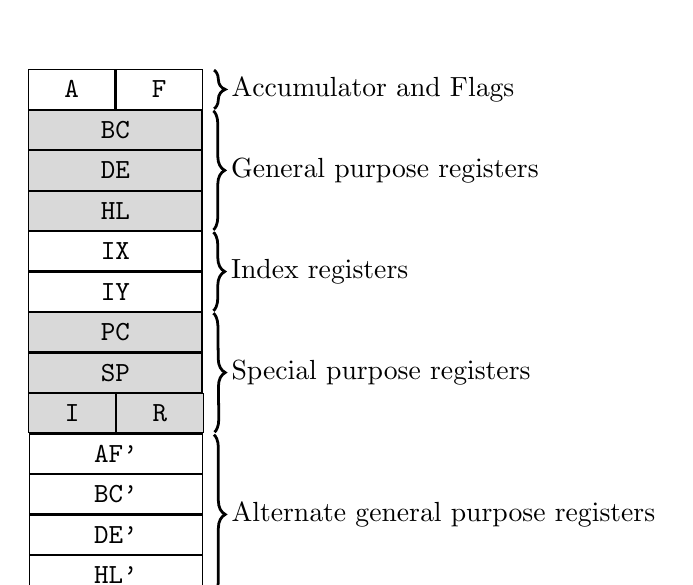
\begin{tikzpicture}[
	framed/.style={draw, font=\ttfamily, minimum width=1.1cm, minimum height=0.5cm},
	filled/.style={framed, fill=PrintableLightGray},
	frameddouble/.style={framed, minimum width=2.2cm},
	filleddouble/.style={filled, minimum width=2.2cm},
	desc/.style={midway,xshift=1.5ex,anchor=west},
	curly/.style={
		decorate,
		decoration={brace,amplitude=5pt,raise=3pt},
		line width=1pt,
		yshift=0pt,
		shorten >=1pt,
		shorten <=1pt
	}
]

	\node[framed] (a) {A};
	\node[framed, right=0pt of a] (f) {F};
	\draw[curly] (f.north east) -- (f.south east) node[desc] {Accumulator and Flags};

	\node[filleddouble, below=0pt of a.south east] (bc) {BC};
	\node[filleddouble, below=0pt of bc] (de) {DE};
	\node[filleddouble, below=0pt of de] (hl) {HL};
	\draw[curly] (bc.north east) -- (hl.south east) node[desc] {General purpose registers};

	\node[frameddouble, below=0pt of hl] (ix) {IX};
	\node[frameddouble, below=0pt of ix] (iy) {IY};
	\draw[curly] (ix.north east) -- (iy.south east) node[desc] {Index registers};

	\node[filleddouble, below=0pt of iy] (pc) {PC};
	\node[filleddouble, below=0pt of pc] (sp) {SP};
	\node[filled, below=0pt of sp.south west, anchor=north west] (i) {I};
	\node[filled, right=0pt of i] (r) {R};
	\draw[curly] (pc.north east) -- (r.south east) node[desc] {Special purpose registers};

	\node[frameddouble, below=0pt of i.south east] (afe) {AF'};
	\node[frameddouble, below=0pt of afe] (bce) {BC'};
	\node[frameddouble, below=0pt of bce] (dee) {DE'};
	\node[frameddouble, below=0pt of dee] (hle) {HL'};
	\draw[curly] (afe.north east) -- (hle.south east) node[desc] {Alternate general purpose registers};

\end{tikzpicture}


\subsection{Flags}
\label{z80_flags}

The conventional way of denoting the flags is with one letter, ``C'' for the carry flag for example. It could be confused with the C register, so I've chosen to use the ``CF'' notation for flags (except ``P'' which uses ``PV'' notation due to having dual-purpose, either as parity or overflow). And for YF and XF the same notation is used in MAME\footnote{\url{http://www.mame.net/}}.

\begin{tabular}{|l|c|c|c|c|c|c|c|c|} 
	\hline
	bit & 7 & 6 & 5 & 4 & 3 & 2 & 1 & 0 \instrt\instrb \\
	\hline
	flag & SF & ZF & YF & HF & XF & PF & NF & CF \instrt\instrb \\ 
	\hline
\end{tabular}

\begin{description}

	\item[SF]
	Set if the 2-complement value is negative; simply a copy of the most significant bit.

	\item[ZF]
	Set if the result is zero.

	\item[YF]
	A copy of bit 5 of the result.

	\item[HF]
	The half-carry of an addition/subtraction (from bit 3 to 4). Needed for BCD correction with {\tt DAA}.

	\item[XF]
	A copy of bit 3 of the result.

	\item[PV]
	This flag can either be the parity of the result (PF), or the 2-complement signed overflow (VF): set if 2-complement value doesn't fit in the register.

	\item[NF]
	Shows whether the last operation was an addition (0) or a subtraction (1). This information is needed for {\tt DAA}.\footnote{Wouldn't it be better to have separate instructions for {\tt DAA} after addition and subtraction, like the 80x86 has instead of sacrificing a bit in the flag register?}

	\item[CF]
	The carry flag, set if there was a carry after the most significant bit.

\end{description}


\section{Undocumented Opcodes}

There are quite a few undocumented opcodes/instructions. This section should describe every possible opcode so you know what will be executed, whatever the value of the opcode is.

The following prefixes exist: {\tt CB}, {\tt ED}, {\tt DD}, {\tt FD}, {\tt DDCB} and {\tt FDCB}. Prefixes change the way the following opcodes are interpreted. All instructions without a prefix (not a value of one the above) are single-byte opcodes (without the operand, that is), which are documented in the official documentation.


\subsection{CB Prefix \cite{gerton}}
\label{z80_undocumented_prefix_cb}

An opcode with a {\tt CB} prefix is a rotate, shift or bit test/set/reset instruction. A few instructions are missing from the official list, for example {\tt SLL} (Shift Logical Left). It works like {\tt SLA}, for one exception: it sets bit 0 ({\tt SLA} resets it).

\TwoColumnInstructions{
	\TwoColumnInstr{CB30}{SLL B}
	\TwoColumnInstr{CB31}{SLL C}
	\TwoColumnInstr{CB32}{SLL D}
	\TwoColumnInstr{CB33}{SLL E}
}{
	\TwoColumnInstr{CB34}{SLL H}
	\TwoColumnInstr{CB35}{SLL L}
	\TwoColumnInstr{CB36}{SLL (HL)}
	\TwoColumnInstr{CB37}{SLL A}
}

\subsection{DD Prefix \cite{gerton}}

In general, the instruction following the {\tt DD} prefix is executed as is, but if the {\tt HL} register is supposed to be used the {\tt IX} register is used instead. Here are the rules:

\begin{itemize}[topsep=1pt,itemsep=1pt]
	\item Any usage of {\tt HL} is treated as an access to {\tt IX} (except {\tt EX DE,HL} and {\tt EXX} and the {\tt ED} prefixed instructions that use {\tt HL}).
	
	\item Any access to {\tt (HL)} is changed to {\tt (IX+d)}, where ``d'' is a signed displacement byte placed after the main opcode - except {\tt JP (HL)}, which isn't indirect anyway. The mnemonic should be {\tt JP HL}.
	
	\item Any access to {\tt H} is treated as an access to {\tt IX\High} (the high byte of {\tt IX}) except if {\tt (IX+d)} is used as well.
	
	\item Any access to {\tt L} is treated as an access to {\tt IX\Low} (the low byte of {\tt IX}) except if {\tt (IX+d)} is used as well.
	
	\item A {\tt DD} prefix before a {\tt CB} selects a completely different instruction set, see section {\XRef{z80_undocumented_prefix_cbdd}}.
\end{itemize}

Some examples:

\TwoColumnInstructions[p{2.3cm}][0.4]{
	\TwoColumnInstr{\rm Without}{\rm With {\tt DD} prefix}
	\TwoColumnInstr{LD H, (HL)}{LD H, (IX+d)}
	\TwoColumnInstr{LD H, A}{LD IXH, A}
	\TwoColumnInstr{LD L, H}{LD IXL, IXH}
}{
	\TwoColumnInstr{\rm Without}{\rm With {\tt DD} prefix}
	\TwoColumnInstr{JP (HL)}{JP (IX)}
	\TwoColumnInstr{LD DE, 0}{LD DE, 0}
	\TwoColumnInstr{LD HL, 0}{LD IX, 0}
}


\subsection{ED Prefix \cite{gerton}}

There are a number of undocumented {\tt EDxx} instructions, of which most are duplicates of documented instructions. Any instruction not listed here has no effect (same as 2 {\tt NOP}s). \See{**} indicates undocumented instruction:

\TwoColumnInstructions{
	\TwoColumnInstr{ED40}{IN B, (C)}
	\TwoColumnInstr{ED41}{OUT (C), B}
	\TwoColumnInstr{ED42}{SBC HL, BC}
	\TwoColumnInstr{ED43}{LD (nn), BC}
	\TwoColumnInstr{ED44}{NEG}
	\TwoColumnInstr{ED45}{RETN}
	\TwoColumnInstr{ED46}{IM 0}
	\TwoColumnInstr{ED47}{LD I, A}
	\TwoColumnInstr{ED48}{IN C, (C)}
	\TwoColumnInstr{ED49}{OUT (C), C}
	\TwoColumnInstr{ED4A}{ADC HL, BC}
	\TwoColumnInstr{ED4B}{LD BC, (nn)}
	\TwoColumnInstr{ED4C}{NEG\See{**}}
	\TwoColumnInstr{ED4D}{RETI}
	\TwoColumnInstr{ED4E}{IM 0\See{**}}
	\TwoColumnInstr{ED4F}{LD R, A}
}{
	\TwoColumnInstr{ED50}{IN D, (C)}
	\TwoColumnInstr{ED51}{OUT (C), D}
	\TwoColumnInstr{ED52}{SBC HL, DE}
	\TwoColumnInstr{ED53}{LD (nn), DE}
	\TwoColumnInstr{ED54}{NEG\See{**}}
	\TwoColumnInstr{ED55}{RETN\See{**}}
	\TwoColumnInstr{ED56}{IM 1}
	\TwoColumnInstr{ED57}{LD A, I}
	\TwoColumnInstr{ED58}{IN E, (C)}
	\TwoColumnInstr{ED59}{OUT (C), E}
	\TwoColumnInstr{ED5A}{ADC HL, DE}
	\TwoColumnInstr{ED5B}{LD DE, (nn)}
	\TwoColumnInstr{ED5C}{NEG\See{**}}
	\TwoColumnInstr{ED5D}{RETN\See{**}}
	\TwoColumnInstr{ED5E}{IM 2}
	\TwoColumnInstr{ED5F}{LD A, R}
}

\TwoColumnInstructions{
	\TwoColumnInstr{ED60}{IN H, (C)}
	\TwoColumnInstr{ED61}{OUT (C), H}
	\TwoColumnInstr{ED62}{SBC HL, HL}
	\TwoColumnInstr{ED63}{LD (nn), HL}
	\TwoColumnInstr{ED64}{NEG\See{**}}
	\TwoColumnInstr{ED65}{RETN\See{**}}
	\TwoColumnInstr{ED66}{IM 0\See{**}}
	\TwoColumnInstr{ED67}{RRD}
	\TwoColumnInstr{ED68}{IN L, (C)}
	\TwoColumnInstr{ED69}{OUT (C), L}
	\TwoColumnInstr{ED6A}{ADC HL, HL}
	\TwoColumnInstr{ED6B}{LD HL, (nn)}
	\TwoColumnInstr{ED6C}{NEG\See{**}}
	\TwoColumnInstr{ED6D}{RETN\See{**}}
	\TwoColumnInstr{ED6E}{IM 0\See{**}}
	\TwoColumnInstr{ED6F}{RLD}
}{
	\TwoColumnInstr{ED70}{IN (C) / IN F, (C)\See{**}}
	\TwoColumnInstr{ED71}{OUT (C), 0\See{**}}
	\TwoColumnInstr{ED72}{SBC HL, SP}
	\TwoColumnInstr{ED73}{LD (nn), SP}
	\TwoColumnInstr{ED74}{NEG\See{**}}
	\TwoColumnInstr{ED75}{RETN\See{**}}
	\TwoColumnInstr{ED76}{IM 1\See{**}}
	\TwoColumnInstr{ED77}{NOP\See{**}}
	\TwoColumnInstr{ED78}{IN A, (C)}
	\TwoColumnInstr{ED79}{OUT (C), A}
	\TwoColumnInstr{ED7A}{ADC HL, SP}
	\TwoColumnInstr{ED7B}{LD SP, (nn)}
	\TwoColumnInstr{ED7C}{NEG\See{**}}
	\TwoColumnInstr{ED7D}{RETN\See{**}}
	\TwoColumnInstr{ED7E}{IM 2\See{**}}
	\TwoColumnInstr{ED7F}{NOP\See{**}}
}

The {\tt ED70} instruction reads from I/O port {\tt C}, but does not store the result. It just affects the flags like the other {\tt IN x,(C)} instructions. {\tt ED71} simply outs the value 0 to I/O port {\tt C}.

The {\tt ED63} is a duplicate of the 22 opcode ({\tt LD (nn),HL}) and similarly {\tt ED6B} is a duplicate of the {\tt 2A} opcode ({\tt LD HL,(nn)}). Of course the timings are different. These instructions are listed in the official documentation.

\pagebreak
According to Gerton Lunter\footnote{\email{gerton}{math.rug}{nl}}:

\begin{quote}
	The instructions {\tt ED 4E} and {\tt ED 6E} are {\tt IM 0} equivalents: when {\tt FF} was put on the bus (physically) at interrupt time, the Spectrum continued to execute normally, whereas when an {\tt EF} ({\tt RST \$28}) was put on the bus it crashed, just as it does in that case when the Z80 is in the official interrupt mode 0. In {\tt IM 1} the Z80 just executes a {\tt RST \$38} (opcode {\tt FF}) no matter what is on the bus.
\end{quote}

All the {\tt RETI/RETN} instructions are the same, all like the {\tt RETN} instruction. So they all, including {\tt RETI}, copy {\tt IFF2} to {\tt IFF1}. See section \XRef{z80_interrupts_flipflop} for more information on {\tt RETI} and {\tt RETN} and {\tt IM x}.


\subsection{FD Prefix \cite{gerton}}

This prefix has the same effect as the {\tt DD} prefix, though {\tt IY} is used instead of {\tt IX}.  Note {\tt LD IXL}, {\tt IYH} is not possible: only {\tt IX} or {\tt IY} is accessed in one instruction, never both.


\subsection{DDCB Prefix}
\label{z80_undocumented_prefix_cbdd}

The undocumented {\tt DDCB} instructions store the result (if any) of the operation in one of the seven all-purpose registers. Which one depends on the lower 3 bits of the last byte of the opcode (not operand, so not the offset).

\TwoColumnInstructions{
	\TwoColumnInstr{000}{B}
	\TwoColumnInstr{001}{C}
	\TwoColumnInstr{010}{D}
	\TwoColumnInstr{011}{E}
}{
	\TwoColumnInstr{100}{H}
	\TwoColumnInstr{101}{L}
	\TwoColumnInstr{110}{\normalfont{(none: documented opcode)}}
	\TwoColumnInstr{111}{A}
}

The documented {\tt DDCB0106} is {\tt RLC (IX+\$01)}. So, clear the lower three bits ({\tt DDCB0100}) and something is done to register {\tt B}. The result of the {\tt RLC} (which is stored in {\tt (IX+\$01)}) is now also stored in register {\tt B}. Effectively, it does the following:

\begin{tcblisting}{}
	LD B, (IX+&01)
	RLC B
	LD (IX+&01), B
\end{tcblisting}

So you get double value for money. The result is stored in {\tt B} and {\tt (IX+\$01)}. The most common notation is: {\tt RLC (IX+\$01), B}

I've once seen this notation:

\begin{tcblisting}{}
	RLC (IX+&01)
	LD B, (IX+&01)
\end{tcblisting}

That's not correct: {\tt B} contains the rotated value, even if {\tt (IX+\$01)} points to ROM.

The {\tt DDCB} {\tt SET} and {\tt RES} instructions do the same thing as the shift/rotate instructions:

\TwoColumnInstructions[p{2.2cm}][0.9]{
	\TwoColumnInstr{DDCB10C0}{SET 0, (IX+\$10), B}
	\TwoColumnInstr{DDCB10C1}{SET 0, (IX+\$10), C}
	\TwoColumnInstr{DDCB10C2}{SET 0, (IX+\$10), D}
	\TwoColumnInstr{DDCB10C3}{SET 0, (IX+\$10), E}
	\TwoColumnInstr{DDCB10C4}{SET 0, (IX+\$10), H}
	\TwoColumnInstr{DDCB10C5}{SET 0, (IX+\$10), L}
	\TwoColumnInstr{DDCB10C6}{SET 0, (IX+\$10) {\rm - documented instruction}}
	\TwoColumnInstr{DDCB10C7}{SET 0, (IX+\$10), A}
}{}

So for example with the last instruction, the value of {\tt (IX+\$10)} with bit 0 set is also stored in register {\tt A}.

The {\tt DDCB} {\tt BIT} instructions do not store any value; they merely test a bit. That's why the undocumented {\tt DDCB} {\tt BIT} instructions are no different from the official ones:

\TwoColumnInstructions[p{2.2cm}][0.9]{
	\TwoColumnInstr{DDCB d 78}{BIT 7, (IX+d)}
	\TwoColumnInstr{DDCB d 79}{BIT 7, (IX+d)}
	\TwoColumnInstr{DDCB d 7A}{BIT 7, (IX+d)}
	\TwoColumnInstr{DDCB d 7B}{BIT 7, (IX+d)}
	\TwoColumnInstr{DDCB d 7C}{BIT 7, (IX+d)}
	\TwoColumnInstr{DDCB d 7D}{BIT 7, (IX+d)}
	\TwoColumnInstr{DDCB d 7E}{BIT 7, (IX+d) {\rm - documented instruction}}
	\TwoColumnInstr{DDCB d 7F}{BIT 7, (IX+d)}
}{}


\subsection{FDCB Prefixes}

Same as for the {\tt DDCB} prefix, though {\tt IY} is used instead of {\tt IX}.


\subsection{Combinations of Prefixes}

This part may be of some interest to emulator coders. Here we define what happens if strange sequences of prefixes appear in the instruction cycle of the Z80.

If {\tt CB} or {\tt ED} is encountered, that byte plus the next make up an instruction. {\tt FD} or {\tt DD} should be seen as prefix setting a flag which says ``use {\tt IX} or {\tt IY} instead of {\tt HL}'', and not an instruction. In a large sequence of {\tt DD} and {\tt FD} bytes, it is the last one that counts. Also any other byte (or instruction) resets this flag.

{\tt {\qquad}FD DD 00 21 00 10{\qquad}NOP NOP NOP LD HL, \$1000}




\section{Undocumented Effects}

\subsection{BIT Instructions}
\label{z80_undocumented_flags_bit}

{\tt BIT n,r} behaves much like {\tt AND r,2{\raisebox{1ex}{n}}} with the result thrown away, and CF flag unaffected. Compare {\tt BIT 7,A} with {\tt AND \$80}: flag YF and XF are reset, SF is set if bit 7 was actually set; ZF is set if the result was 0 (bit was reset), and PV is effectively set if ZF is set (the result of the AND leaves either no bits set (PV set - parity even) or one bit set (PV reset - parity odd). So the rules for the flags are:

\begin{description}
	\item[SF flag]
	Set if n = 7 and tested bit is set.

	\item[ZF flag]
	Set if the tested bit is reset.

	\item[YF flag]
	Set if n = 5 and tested bit is set.

	\item[HF flag]
	Always set.

	\item[XF flag]
	Set if n = 3 and tested bit is set.

	\item[PV flag]
	Set just like ZF flag.

	\item[NF flag]
	Always reset. 

	\item[CF flag]
	Unchanged.

\end{description}

This is where things start to get strange. With the {\tt BIT n,(IX+d)} instructions, the flags behave just like the {\tt BIT n,r} instruction, except for YF and XF. These are not copied from the result but from something completely different, namely bit 5 and 3 of the high byte of {\tt IX+d} (so {\tt IX} plus the displacement).

Things get more bizarre with the {\tt BIT n,(HL)} instruction. Again, except for YF and XF, the flags are the same. YF and XF are copied from some sort of internal register. This register is related to 16-bit additions. Most instructions do not change this register. Unfortunately, I haven't tested all instructions yet, but here is the list so far:

\begin{tabularx}{\linewidth}{@{}lX}
	{\tt ADD HL, xx}
		& Use high byte of {\tt HL}, ie. {\tt H} before the addition. \\

	{\tt LD r, (IX+d)}
		& Use high byte of the resulting address {\tt IX+d}. \\

	{\tt JR d}
		& Use high byte target address of the jump. \\

	{\tt LD r, r'}
		& Doesn't change this register. \\
\end{tabularx}

Any help here would be most appreciated!


\pagebreak
\subsection{Memory Block Instructions \cite{mrison}}
\label{z80_undocumented_instructions_memory_block}

The {\tt LDI}/{\tt LDIR}/{\tt LDD}/{\tt LDDR} instructions affect the flags in a strange way. At every iteration, a byte is copied. Take that byte and add the value of register {\tt A} to it. Call that value {\tt n}. Now, the flags are:

\begin{description}
 
	\item[YF flag]
	A copy of bit 1 of n.

	\item[HF flag]
	Always reset.

	\item[XF flag]
	A copy of bit 3 of n.

	\item[PV flag]
	Set if BC not 0.

	\item[SF, ZF, CF flags]
	These flags are unchanged.

\end{description}

And now for {\tt CPI}/{\tt CPIR}/{\tt CPD}/{\tt CPDR}. These instructions compare a series of bytes in memory to register {\tt A}. Effectively, it can be said they perform {\tt CP (HL)} at every iteration. The result of that comparison sets the HF flag, which is important for the next step. Take the value of register {\tt A}, subtract the value of the memory address, and finally subtract the value of HF flag, which is set or reset by the hypothetical {\tt CP (HL)}. So, {\tt n=A-(HL)-HF}.

\begin{description}

	\item[SF, ZF, HF flags]
	Set by the hypothetical {\tt CP (HL)}.

	\item[YF flag]
	A copy of bit 1 of {\tt n}.

	\item[XF flag]
	A copy of bit 3 of {\tt n}.

	\item[PV flag]
	Set if BC is not 0.

	\item[NF flag]
	Always set.

	\item[CF flag]
	Unchanged.

\end{description}


\subsection{I/O Block Instructions}
\label{z80_undocumented_instructions_io_block}

These are the most bizarre instructions, as far as the flags are concerned. Ramsoft found all of the flags. The ``out'' instructions behave differently than the ``in'' instructions, which doesn't make the CPU very symmetrical. 

First of all, all instructions affect the following flags:

\begin{description}

	\item[SF, ZF, YF, XF flags]
	Affected by decreasing register B, as in {\tt DEC B}.

	\item[NF flag]
	A copy of bit 7 of the value read from or written to an I/O port.

\end{description}

\pagebreak % we want to keep this paragraph with description below to avoid page flipping
And now the for {\tt OUTI}/{\tt OTIR}/{\tt OUTD}/{\tt OTDR} instructions. Take the state of the {\tt L} after the increment or decrement of HL; add the value written to the I/O port; call that {\tt k} for now. If {\tt k} $>$ 255, then the CF and HF flags are set. The PV flag is set like the parity of {\tt k} bitwise and'ed with 7, bitwise xor'ed with {\tt B}.

\begin{description}

	\item[HF and CF]
	Both set if {\tt ((HL) + L  $>$ 255)}

	\item[PV]
	The parity of {\tt ((((HL) + L) $\wedge$ 7) $\veebar$ B)}

\end{description}

{\tt INI}/{\tt INIR}/{\tt IND}/{\tt INDR} use the {\tt C} register instead of the {\tt L} register. There is a catch though, because not the value of {\tt C} is used, but {\tt C + 1} if it's {\tt INI}/{\tt INIR} or {\tt C - 1} if it's {\tt IND}/{\tt INDR}. So, first of all {\tt INI}/{\tt INIR}:

\begin{description}

	\item[HF and CF]
	Both set if {\tt ((HL) + ((C + 1) $\wedge$ 255)  $\veebar$ 255)}

	\item[PF]
	The parity of {\tt (((HL) + ((C + 1) $\wedge$ 255)) $\wedge$ 7) $\veebar$ B)}

\end{description}

And last {\tt IND}/{\tt INDR}:

\begin{description}

	\item[HF and CF]
	Both set if {\tt ((HL) + ((C - 1) $\wedge$ 255) $>$ 255)}

	\item[PF]
	The parity of {\tt (((HL) + ((C - 1) $\wedge$ 255)) $\wedge$ 7) $\veebar$ B)}

\end{description}


\subsection{16 Bit I/O ports}

Officially the Z80 has an 8-bit I/O port address space. When using the I/O ports, the 16 address lines are used. And in fact, the high 8 bits do have some value, so you can use 65536 ports after all. {\tt IN r, (C)}, {\tt OUT (C), r}, and the block I/O instructions actually place the entire {\tt BC} register on the address bus. Similarly {\tt IN A, (n)} and {\tt OUT (n), A} put {\tt A $\times$256 + n} on the address bus.

The {\tt INI}, {\tt INIR}, {\tt IND} and {\tt INDR} instructions use {\tt BC} before decrementing {\tt B}, and the {\tt OUTI}, {\tt OTIR}, {\tt OUTD} and {\tt OTDR} instructions use {\tt BC} after decrementing.


\subsection{Block Instructions}

The repeated block instructions simply decrement the {\tt PC} by two so the instruction is simply re-executed. So interrupts can occur during block instructions. So, {\tt LDIR} is simply {\tt LDI} + if {\tt BC} is not {\tt 0}, decrement {\tt PC} by {\tt 2}.


\subsection{16 Bit Additions}

The 16-bit additions are a bit more complicated than the 8-bit ones. Since the Z80 is an 8-bit CPU, 16-bit additions are done in two stages: first, the lower bytes are added, then the two higher bytes. The SF, YF, HF, XF flags are affected by the second (high) 8-bit addition. ZF is set if the whole 16-bit result is 0.


\subsection{DAA Instruction}
\label{z80_undocumented_instruction_daa}

This instruction is useful when you're using BCD values. After addition or subtraction, {\tt DAA} corrects the value back to BCD again.  Note that it uses the CF flag, so it cannot be used after {\tt INC} and {\tt DEC}.

Stefano Donati from Ramsoft\footnote{http://www.ramsoft.bbk.org/} has found the tables which describe the {\tt DAA} operation. The input is the A register and the CF, NF, HF flags. The result is as follows:

{
	\footnotesize

	\begin{tabular}{b{5.8cm}b{4.8cm}b{4.8cm}}
		Depending on the NF flag, the ``diff'' from this table must be added (NF is reset) or subtracted (NF is set) to {\tt A}:
		&
		CF flag is affected:
		&
		NF flag is affected: \\
	\end{tabular}

	\begin{tabular}{p{5.8cm}p{4.8cm}p{4.8cm}}

		% ----------------------------------
		% | NF | CF |  hi | HF |  lo | add |
		% |----|----|-----|----|-----|-----|
		% |  0 |  0 | 0-9 |  0 | 0-9 |  00 |
		% |  0 |  0 | 0-9 |  1 | 0-9 |  06 |
		% |  0 |  0 | 0-8 |  * | a-f |  06 |
		% |  0 |  0 | a-f |  0 | 0-9 |  60 |
		% |  0 |  1 |  *  |  0 | 0-9 |  60 |
		% |  0 |  1 |  *  |  1 | 0-9 |  66 |
		% |  0 |  1 |  *  |  * | a-f |  66 |
		% |  0 |  0 | 9-f |  * | a-f |  66 |
		% |  0 |  0 | a-f |  1 | 0-9 |  66 |
		% ----------------------------------
		% |  1 |  0 | 0-9 |  0 | 0-9 |  00 |
		% |  1 |  0 | 0-9 |  1 | 0-9 |  fa |
		% |  1 |  0 | 0-8 |  * | a-f |  fa |
		% |  1 |  0 | a-f |  0 | 0-9 |  a0 |
		% |  1 |  1 |  *  |  0 | 0-9 |  a0 |
		% |  1 |  1 |  *  |  1 | 0-9 |  9a |
		% |  1 |  1 |  *  |  * | a-f |  9a |
		% |  1 |  0 | 9-f |  * | a-f |  9a |
		% |  1 |  0 | a-f |  1 | 0-9 |  9a |
		% ----------------------------------
		{\tt
			\begin{tabular}[t]{c|c|c|c|c}
				   &  high   &    & low    &  \\
				CF &  nibble & HF & nibble & diff \\
				\hline
				0 & 0-9     &  0 & 0-9    &  00  \\
				0 & 0-9     &  1 & 0-9    &  06  \\
				0 & 0-8     &  * & A-F    &  06  \\
				0 & A-F     &  0 & 0-9    &  60  \\
				1 &  *      &  0 & 0-9    &  60  \\
				1 &  *      &  1 & 0-9    &  66  \\
				1 &  *      &  * & A-F    &  66  \\
				0 & 9-F     &  * & A-F    &  66  \\
				0 & A-F     &  1 & 0-9    &  66  \\
				\hline
			\end{tabular}
		}

		&

		% ------------------------
		% | CF |  hi |  lo | CF' |
		% |----|-----|-----|-----|
		% |  0 | 0-9 | 0-9 |  0  |
		% |  0 | 0-8 | a-f |  0  |
		% |  0 | 9-f | a-f |  1  |
		% |  0 | a-f | 0-9 |  1  |
		% |  1 |  *  |  *  |  1  |
		% ------------------------
		{\tt
			\begin{tabular}[t]{c|c|c|c}
				   & high   & low    & \\
				CF & nibble & nibble & CF' \\ 	
				\hline
				0 & 0-9    & 0-9    &  0  \\
				0 & 0-8    & A-F    &  0  \\
				0 & 9-F    & A-F    &  1  \\
				0 & A-F    & 0-9    &  1  \\
				1 &  *     &  *     &  1  \\ 
				\hline
			\end{tabular}
		}

		&
		
		% -----------------------
		% | NF | HF |  lo | HF' |
		% |----|----|-----|-----|
		% |  0 |  * | 0-9 |  0  |
		% |  0 |  * | a-f |  1  |
		% -----------------------
		% |  1 |  0 |  *  |  0  |
		% |  1 |  1 | 6-f |  0  |
		% |  1 |  1 | 0-5 |  1  |
		% -----------------------
		{\tt
			\begin{tabular}[t]{c|c|c|c}
				   &    & low    & \\
				NF & HF & nibble & HF' \\ 
				\hline
				0 &  * & 0-9    &  0  \\
				0 &  * & A-F    &  1  \\
				1 &  0 &  *     &  0  \\
				1 &  1 & 6-F    &  0  \\
				1 &  1 & 0-5    &  1  \\ 
				\hline
			\end{tabular}
		}
		
		\\

	\end{tabular}
}

SF, YF, XF are copies of bit 7, 5, 3 of the result respectively; ZF is set according to the result and NF is always unchanged.


\section{Interrupts}
\label{z80_interrupts}

There are two types of interrupts, maskable and non-maskable. The maskable type is ignored if {\tt IFF1} is reset. Non-maskable interrupts (NMI) will are always accepted, and they have a higher priority, so if both are requested at the same time, the NMI will be accepted first.

For the interrupts, the following things are important: interrupt Mode (set with the {\tt IM 0, IM 1, IM 2} instructions), the interrupt flip-flops ({\tt IFF1} and {\tt IFF2}), and the {\tt I} register. When a maskable interrupt is accepted, the external device can put a value on the data bus.

Both types of interrupts increase the {\tt R} register by one when accepted.


\subsection{Non-Maskable Interrupts (NMI)}

When an NMI is accepted, {\tt IFF1} is reset. At the end of the routine, {\tt IFF1} must be restored (so the running program is not affected). That's why {\tt IFF2} is there; to keep a copy of {\tt IFF1}.

An NMI is accepted when the \NoLinkChipPinLabel{NMI} pin on the Z80 is made low (edge-triggered). The Z80 responds to the change of the line from +5 to 0 - so the interrupt line doesn't have a state, it's just a pulse. When this happens, a call is done to address \MemAddr{0066} and {\tt IFF1} is reset so the routine isn't bothered by maskable interrupts. The routine should end with an {\tt RETN} (RETurn from Nmi) which is just a usual {\tt RET} but also copies {\tt IFF2} to {\tt IFF1}, so the IFFs are the same as before the interrupt.

You can check whether interrupts were disabled or not during an NMI by using the {\tt LD A,I} or {\tt LD A,R} instruction. These instructions copy {\tt IFF2} to the PV flag.

Accepting an NMI costs 11 t-states.


\subsection{Maskable Interrupts (INT)}

If the \NoLinkChipPinLabel{INT} line is low and {\tt IFF1} is set, a maskable interrupt is accepted - whether or not the last interrupt routine has finished. That's why you should not enable interrupts during such a routine, and make sure that the device that generated it has put the \NoLinkChipPinLabel{INT} line up again before ending the routine. So unlike NMI interrupts, the interrupt line has a state; it's not a pulse.

When an interrupt is accepted, both {\tt IFF1} and {\tt IFF2} are cleared, preventing another interrupt from occurring which would end up as an infinite loop (and overflowing the stack). What happens next depends on the Interrupt Mode.

A device can place a value on the data bus when the interrupt is accepted. Some computer systems do not utilize this feature, and this value ends up being {\tt \$FF}.

\begin{description}

	\item[Interrupt Mode 0]
	This is the 8080 compatibility mode. The instruction on the bus is executed (usually an {\tt RST} instruction, but it can be anything). {\tt I} register is not used. Assuming it's a {\tt RST} instruction, accepting this takes 13 t-states.

	\item[Interrupt Mode 1]
	This is the 8080 compatibility mode. The instruction on the bus is executed (usually an {\tt RST} instruction, but it can be anything). {\tt I} register is not used. Assuming it's a {\tt RST} instruction, accepting this takes 13 t-states.

	\item[Interrupt Mode 2]
	A call is made to the address read from memory. What address is read from is calculated as follows: $(I\ register) \times 256 + (value\ on\ bus)$. Zilog's user manual states (very convincingly) that the least significant bit of the address is always 0, so they calculate the address that is read from as: $(I\ register) \times 256 + (value\ on\ bus \wedge \mathtt{\$FE})$. I have tested this and it's not correct. Of course, a word (two bytes) is read, making the address where the call is made to. In this way, you can have a vector table for interrupts. Accepting this interrupt type costs 19 t-states.

\end{description}

At the end of a maskable interrupt, the interrupts should be enabled again. You can assume that was the state of the IFFs because otherwise the interrupt wasn't accepted. So, an interrupt routine always ends with an {\tt EI} and a {\tt RET} ({\tt RETI} according to the official documentation, more about that later):

\begin{tcblisting}{}
InterruptRoutine:
	...
	EI
	RETI or RET
\end{tcblisting}

Note a fact about {\tt EI}: a maskable interrupt isn't accepted directly after it, so the next opportunity for an interrupt is after the {\tt RETI}. This is very useful; if the \NoLinkChipPinLabel{INT} line is still low, an interrupt is accepted again.  If this happens a lot and the interrupt is generated before the {\tt RETI}, the stack could overflow (since the routine would be called again and again). But this property of {\tt EI} prevents this.

{\tt DI} is not necessary at the start of the interrupt routine: the interrupt flip-flops are cleared when accepting the interrupt.

You can use {\tt RET} instead of {\tt RETI}, depending on the hardware setup. {\tt RETI} is only useful if you have something like a Z80 PIO to support daisy-chaining: queuing interrupts. The PIO can detect that the routine has ended by the opcode of {\tt RETI}, and let another device generate an interrupt. That is why I called all the undocumented {\tt EDxx} {\tt RET} instructions {\tt RETN}: All of them operate alike, the only difference of {\tt RETI} is its specific opcode which the Z80 PIO recognises.


\subsection{Things Affecting the Interrupt Flip-Flops}
\label{z80_interrupts_flipflop}

All the IFF related things are:

\begin{tabular}{llll}
	Accept NMI	& {\tt IFF1}	& {\tt IFF2} \\
	CPU reset	& {\tt 0}		& {\tt 0}\\
	{\tt DI}	& {\tt 0}		& {\tt 0}\\
	{\tt EI}	& {\tt 1}		& {\tt 1}\\
	Accept INT	& {\tt 0}		& {\tt 0}\\
	Accept NMI	& {\tt 0}		& -\\
	{\tt RETI/N}& {\tt IFF2}	& - & All the {\tt EDxx} {\tt RETI/N} instructions\\
	{\tt LD A,I / LD A,R} & - & - & Copies {\tt IFF2} into {\tt PV} flag
\end{tabular}

If you're working with a Z80 system without NMIs (like the MSX), you can forget all about the two separate IFFs; since an NMI isn't ever generated, the two will always be the same. 

Some documentation says that when an NMI is accepted, {\tt IFF1} is first copied into {\tt IFF2} before {\tt IFF1} is cleared. If this is true, the state of {\tt IFF2} is lost after a nested NMI, which is undesirable. Have tested this in the following way: make sure the Z80 is in {\tt EI} mode, generate an NMI. In the NMI routine, wait for another NMI before executing {\tt RETN}. In the second NMI {\tt IFF2} was still set, so {\tt IFF1} is {\em not} copied to {\tt IFF2} when accepting an NMI.

Another interesting fact: I was trying to figure out whether the undocumented {\tt ED} {\tt RET} instructions were {\tt RETN} or {\tt RETI}. I tested this by putting the machine in {\tt EI} mode, wait for an NMI and end with one of the {\tt ED} {\tt RET} instructions. Then execute a {\tt HALT} instruction. If {\tt IFF1} was not restored, the machine would hang but this did not happen with any of the instructions, including the documented {\tt RETI}!

Since every interrupt routine must end with {\tt EI} followed by {\tt RETI} officially, It does not matter that {\tt RETI} copies {\tt IFF2} into IFF1; both are set anyway.


\subsection{HALT Instruction}

The HALT instruction halts the Z80; it does not increase the PC so that the instruction is re-executed until a maskable or non-maskable interrupt is accepted. Only then does the Z80 increase the PC again and continues with the next instruction. During the HALT state, the HALT line is set. The PC is increased before the interrupt routine is called.


\subsection{Where interrupts are accepted}

During the execution of instructions, interrupts won't be accepted. Only {\em between} instructions. This is also true for prefixed instructions.

Directly after an {\tt EI} or {\tt DI} instruction, interrupts aren't accepted. They're accepted again after the instruction after the {\tt EI} ({\tt RET} in the following example). So for example, look at this MSX2 routine that reads a scanline from the keyboard:

\begin{tcblisting}{}
	LD C, A
	DI
	IN A, (&AA)
	AND &F0
	ADD A, C
	OUT (&AA), A
	EI
	IN A, (&A9)
	RET
\end{tcblisting}

You can assume that there never is an interrupt after the {\tt EI}, before the {\tt IN A,(\$A9)} - which would be a problem because the MSX interrupt routine reads the keyboard too.

Using this feature of {\tt EI}, it is possible to check whether it is true that interrupts are never accepted during instructions:

\begin{tcblisting}{}
	DI
	|make sure interrupt is active|
	EI
	|insert instruction to test|
InterruptRoutine:
	|store PC where interrupt was accepted|
	RET
\end{tcblisting}

And yes, for all instructions, including the prefixed ones, interrupts are never accepted during an instruction. Only after the tested instruction. Remember that block instructions simply re-execute themselves (by decreasing the PC with 2) so an interrupt is accepted after each iteration.

Another predictable test: at the ``insert instruction to test'' insert a large sequence of {\tt EI} instructions. Of course, during the execution of the {\tt EI} instructions, no interrupts are accepted. 

\pagebreak % we want to keep this paragraph together on the next page
But now for the interesting stuff. {\tt ED} or {\tt CB} make up instructions, so interrupts are accepted after them. But {\tt DD} and {\tt FD} are prefixes, which only slightly affects the next opcode. If you test a large sequence of {\tt DD}s or {\tt FD}s, the same happens as with the {\tt EI} instruction: no interrupts are accepted during the execution of these sequences.

This makes sense if you think of {\tt DD} and {\tt FD} as a prefix that sets the ``use {\tt IX} instead of {\tt HL}'' or ``use {\tt IY} instead of {\tt HL}'' flag. If an interrupt was accepted after {\tt DD} or {\tt FD}, this flag information would be lost, and:

{\tt 
	{\qquad}DD 21 00 00{\qquad}LD IX, 0
}

could be interpreted as a simple {\tt LD HL,0} if the interrupt was after the last {\tt DD}. Which never happens, so the implementation is correct. Although I haven't tested this, as I imagine the same holds for NMI interrupts.

Also see section \XRef{zx_next_interrupts} for details on handling interrupts on ZX Spectrum Next.


\section{Timing and R register}

\subsection{R register and memory refresh}

During every first machine cycle (beginning of instruction or part of it - prefixes have their own M1 two), the memory refresh cycle is issued. The whole IR register is put on the address bus, and the \NoLinkChipPinLabel{RFSH} pin is lowered.  It's unclear whether the Z80 increases the {\tt R} register before or after putting IR on the bus. 

The {\tt R} register is increased at every first machine cycle (M1). Bit 7 of the register is never changed by this; only the lower 7 bits are included in the addition. So bit 7 stays the same, but it can be changed using the
{\tt LD R,A} instruction.

Instructions without a prefix increase {\tt R} by one. Instructions with an {\tt ED}, {\tt CB}, {\tt DD}, {\tt FD} prefix, increase {\tt R} by two, and so do the {\tt DDCBxxxx} and {\tt FDCBxxxx} instructions (weird enough). Just a stray {\tt DD} or {\tt FD} increases the {\tt R} by one. {\tt LD A,R} and {\tt LD R,A} access the {\tt R} register after it is increased by the instruction itself. 

Remember that block instructions simply decrement the {\tt PC} with two, so the instructions are re-executed. So {\tt LDIR} increases {\tt R} by {\tt BC} $\times$ 2 (note that in the case of {\tt BC} = 0, {\tt R} is increased by \MemAddr{10000} $\times$ 2, effectively 0).

Accepting a maskable or non-maskable interrupt increases the {\tt R} by one.

After a hardware reset, or after power on, the {\tt R} register is reset to 0.

That should cover all there is to say about the {\tt R} register. It is often used in programs for a random value, which is good but of course not truly random.


\pagebreak
\section{Errors in Official Documentation}

Some official Zilog documentation contains errors. Not every documentation has all of these mistakes, so your milage may vary, but these are just things to look out for.

\begin{itemize}

	\item
	The flag affection summary table shows that {\tt LDI}/{\tt LDIR}/{\tt LDD}/{\tt LDDR} instructions leave the SF and ZF in an undefined state. This is not correct; the SF and ZF flags are unaffected.

	\item
	Similarly, the same table shows that {\tt CPI}/{\tt CPIR}/{\tt CPD}/{\tt CPDR} leave the SF and HF flags in an undefined state. Not true, they are affected as defined elsewhere in the documentation.

	\item
	Also, the table says about {\tt INI}/{\tt OUTD}/etc ``Z=0 if B $<>$ 0 otherwise Z=0''; of course the latter should be Z=1.

	\item
	The {\tt INI}/{\tt INIR}/{\tt IND}/{\tt INDR}/{\tt OUTI}/{\tt OUTD}/{\tt OTIR}/{\tt OTDR} instructions do affect the CF flag (some official documentation says they leave it unaffected, important!) and the NF flag isn't always set but may also be reset (see \XRef{z80_undocumented_instructions_io_block} for exact operation).

	\item
	When an NMI is accepted, the {\tt IFF1} isn't copied to {\tt IFF2}. Only {\tt IFF1} is reset.

	\item
	In the 8-bit Load Group, the last two bits of the second byte of the {\tt LD r,(IX + d)} opcode should be 10 and not 01.

	\item
	In the 16-bit Arithmetic Group, bit 6 of the second byte of the {\tt ADD IX,pp} opcode should be 0, not 1.

	\item
	{\tt IN x,(C)} resets the HF flag, it never sets it. Some documentation states it is set according to the result of the operation; this is impossible since no arithmetic is done in this instruction.

\end{itemize}

Note: In zilog's own z80cpu\_um.pdf document, there are a lot of errors, some are very confusing, so I'll mention the ones I have found here:

\begin{itemize}

	\item
	Page 21, figure 2 says ``the Alternative Register Set contains 2 {\tt B'} registers''; this should of course be {\tt B'} and {\tt C'}.

	\item
	Page 26, figure 16 shows very convincingly that ``the least significant bit of the address to read for Interrupt Mode 2 is always 0''. I have tested this and it is not correct, it can also be 1, in my test case the bus contained {\tt \$FF} and the address that was read did not end in {\tt \$FE} but was {\tt \$FF}.
  
\end{itemize}


	% note: for Next chapter, we use `\include{}` for each section; we want each to be treated as its own section, with `\clearpage` etc.
	\chapter{ZX Spectrum Next}

% █████████████████████████████████████████████████████████████████████████
% █░░░░░░██████████░░░░░░█░░░░░░░░░░░░░░█░░░░░░░░██░░░░░░░░█░░░░░░░░░░░░░░█
% █░░▄▀░░░░░░░░░░██░░▄▀░░█░░▄▀▄▀▄▀▄▀▄▀░░█░░▄▀▄▀░░██░░▄▀▄▀░░█░░▄▀▄▀▄▀▄▀▄▀░░█
% █░░▄▀▄▀▄▀▄▀▄▀░░██░░▄▀░░█░░▄▀░░░░░░░░░░█░░░░▄▀░░██░░▄▀░░░░█░░░░░░▄▀░░░░░░█
% █░░▄▀░░░░░░▄▀░░██░░▄▀░░█░░▄▀░░███████████░░▄▀▄▀░░▄▀▄▀░░███████░░▄▀░░█████
% █░░▄▀░░██░░▄▀░░██░░▄▀░░█░░▄▀░░░░░░░░░░███░░░░▄▀▄▀▄▀░░░░███████░░▄▀░░█████
% █░░▄▀░░██░░▄▀░░██░░▄▀░░█░░▄▀▄▀▄▀▄▀▄▀░░█████░░▄▀▄▀▄▀░░█████████░░▄▀░░█████
% █░░▄▀░░██░░▄▀░░██░░▄▀░░█░░▄▀░░░░░░░░░░███░░░░▄▀▄▀▄▀░░░░███████░░▄▀░░█████
% █░░▄▀░░██░░▄▀░░░░░░▄▀░░█░░▄▀░░███████████░░▄▀▄▀░░▄▀▄▀░░███████░░▄▀░░█████
% █░░▄▀░░██░░▄▀▄▀▄▀▄▀▄▀░░█░░▄▀░░░░░░░░░░█░░░░▄▀░░██░░▄▀░░░░█████░░▄▀░░█████
% █░░▄▀░░██░░░░░░░░░░▄▀░░█░░▄▀▄▀▄▀▄▀▄▀░░█░░▄▀▄▀░░██░░▄▀▄▀░░█████░░▄▀░░█████
% █░░░░░░██████████░░░░░░█░░░░░░░░░░░░░░█░░░░░░░░██░░░░░░░░█████░░░░░░█████
% █████████████████████████████████████████████████████████████████████████


\ChapterTOC[]

\pagebreak
\thispagestyle{plain} % use toc style without headers for this explanation page, it better matches chapter start page

With increased CPU speeds, more memory, better graphics, hardware sprites and tiles, to mention just some of the most obvious, ZX Spectrum Next is an exciting platform for the retro programmer.

This chapter represents the bulk of the book. Each topic is discussed in its own section. While the sections are laid out in order - later sections sometimes rely on, or refer to the topics discussed earlier, there's no need to go through them in an orderly fashion. Each section should be quite usable by itself as well. All topics discussed elsewhere are referenced, so you can quickly jump there if needed. If using PDF you can click on the section number to go straight to it. With a printed book though, turning the pages gives you a chance to land on something unrelated, but equally interesting, thus learning something new almost by accident.

One more thing worth mentioning, before leaving you on to explore, are ports and Next registers. You will find the full list in the next section. But that's just a list with a couple of examples on how to read and write them. Still, many ports and registers are described in detail at the end of the sections in which they are first mentioned. Those registers that are relevant for multiple topics are described in the first section they are mentioned in, and then referenced from other sections. Additionally, each port and register that's described in detail, has the reference to that section in the list on the following pages as a convenience. I thought for a while about how to approach this. One way would be to describe the ports and references in a single section, together with their list, and then only reference them elsewhere. But ultimately decided on the format described above for two reasons: descriptions are not comprehensive, only relevant ports and registers have this ``honour''. And secondly, I wanted to keep all relevant material as close together as possible.

\pagebreak
\pagestyle{clean} % all subsequent pages should use clean style with full header

	\section{Ports and Registers}
\label{zx_next_ports}

% ────────────────────────────────────────────────────────────────────────────────
% ─██████████████─██████████████─████████████████───██████████████─██████████████─
% ─██░░░░░░░░░░██─██░░░░░░░░░░██─██░░░░░░░░░░░░██───██░░░░░░░░░░██─██░░░░░░░░░░██─
% ─██░░██████░░██─██░░██████░░██─██░░████████░░██───██████░░██████─██░░██████████─
% ─██░░██──██░░██─██░░██──██░░██─██░░██────██░░██───────██░░██─────██░░██─────────
% ─██░░██████░░██─██░░██──██░░██─██░░████████░░██───────██░░██─────██░░██████████─
% ─██░░░░░░░░░░██─██░░██──██░░██─██░░░░░░░░░░░░██───────██░░██─────██░░░░░░░░░░██─
% ─██░░██████████─██░░██──██░░██─██░░██████░░████───────██░░██─────██████████░░██─
% ─██░░██─────────██░░██──██░░██─██░░██──██░░██─────────██░░██─────────────██░░██─
% ─██░░██─────────██░░██████░░██─██░░██──██░░██████─────██░░██─────██████████░░██─
% ─██░░██─────────██░░░░░░░░░░██─██░░██──██░░░░░░██─────██░░██─────██░░░░░░░░░░██─
% ─██████─────────██████████████─██████──██████████─────██████─────██████████████─
% ────────────────────────────────────────────────────────────────────────────────

\newcommand{\ZXSee}[1]{(see section \PortXRef{#1})}

\subsection{Mapped Spectrum Ports}

\begingroup
	\newcommand{\zxport}[4]{
		\tt {#1} & 
		{\tt \$#2} & 
		\IfEq{#3}{}{}{\tt \%#3} &
		#4\\
	}

	\setlength{\extrarowheight}{5pt}	% a bit more spacing between items for clearer visuals

	\begin{tabularx}{\textwidth}{lllX}
		{\tt RW} & Addr & Mask & Description \\
		
		\hline
		
		\zxport{RW}{103B}{0001 0000 0011 1011}{Sets and reads the I2C SCL line}
		\zxport{RW}{113B}{0001 0001 0011 1011}{Sets and reads the I2C SDA line}
		\zxport{RW}{123B}{0001 0010 0011 1011}{Enables layer 2 and controls paging of layer 2 screen into lower memory \ZXSee{123B}}
		\zxport{RW}{133B}{0001 0011 0011 1011}{Sends byte to serial port. Read tells if data is available in RX buffer}
		\zxport{RW}{143B}{0001 0100 0011 1011}{Reads data from serial port, write sets the baud rate}
		\zxport{RW}{153B}{0001 0101 0011 1011}{Configuration of UART interfaces}
		\zxport{-W}{1FFD}{0001 ---- ---- --0-}{Controls ROM paging and special paging options from the +2a/+3 \ZXSee{1FFD}}
		\zxport{RW}{243B}{0010 0100 0011 1011}{Selects active port for TBBlue/Next feature configuration \ZXSee{243B}}
		\zxport{RW}{253B}{0010 0101 0011 1011}{Reads and/or writes the selected TBBlue control register \ZXSee{253B}}
		\zxport{RW}{303B}{0011 0000 0011 1011}{Sets active sprite-attribute index and pattern-slot index, reads sprite status \ZXSee{303B}}
		\zxport{-W}{7FFD}{01-- ---- ---- --0-}{Selects active RAM, ROM, and displayed screen \ZXSee{7FFD}}
		\zxport{-W}{BFFD}{10-- ---- ---- --0-}{Writes to the selected register of the selected sound chip \ZXSee{BFFD}}
		\zxport{-W}{DFFD}{1101 1111 1111 1101}{Provides additional bank select bits for extended memory \ZXSee{DFFD}}
		\zxport{R-}{FADF}{---- ---0 --0- ----}{Reads buttons on Kempston Mouse}
		\zxport{R-}{FBDF}{---- -0-1 --0- ----}{X coordinate of Kempston Mouse, 0-255}
		\zxport{R-}{FFDF}{---- -1-1 --0- ----}{Y coordinate of Kempston Mouse, 0-192}
		\zxport{-W}{FFFD}{11-- ---- ---- --0-}{Controls stereo channels and selects active sound chip and sound chip channel \ZXSee{FFFD}}

	\end{tabularx}

	\pagebreak
	\vspace*{9ex}
	\begin{tabularx}{\textwidth}{lllX}
		{\tt RW} & Addr & Mask & Description \\
		
		\hline

		\zxport{RW}{xx0B}{---- ---- 0000 1011}{Controls Z8410 DMA chip via MB02 standard \ZXSee{xx0B}}
		\zxport{R-}{xx1F}{---- ---- 0001 1111}{Reads movement of joysticks using Kempston interface}
		\zxport{RW}{xx37}{---- ---- ---- ----}{Kempston interface second joystick variant and controls joystick I/O}
		\zxport{-W}{xx57}{---- ---- 0101 0111}{Uploads sprite positions, visibility, colour type and effect flags \ZXSee{xx5B}}
		\zxport{-W}{xx5B}{---- ---- 0101 1011}{Used to upload the pattern of the selected sprite \ZXSee{xx5B}}
		\zxport{RW}{xx6B}{---- ---- 0110 1011}{Controls zxnDMA chip \ZXSee{xx6B}}
		\zxport{-W}{xxDF}{---- ---- --01 1111}{Output to SpecDrum DAC}
		\zxport{RW}{xxFE}{xxxx xxxx ---- ---0}{Reading with particular high bytes returns keyboard status \ZXSee{xxFE}, write changes border colour and base Spectrum audio settings \ZXSee{xxFEWrite}}
		\zxport{RW}{xxFF}{---- ---- ---- ----}{Controls Timex Sinclair video modes and colours in hi-res mode. Readable when bit 2 of \PortTextXRef{08} is set}

	\end{tabularx}
\endgroup


\pagebreak

\subsection{Next/TBBlue Feature Control Registers}
\label{zx_next_tbblue_registers}

Specific features of the Next are controlled via these register numbers, accessed through ports \PortTextXRef[]{243B} and \PortTextXRef[]{253B} (see page \PortPage{243B} for details). All registers can also be written to directly with the {\tt NEXTREG} instruction.

\begingroup
	\NewDocumentEnvironment{tbbluereg}{ +b }{
		\begin{tabularx}{\textwidth}{llX}
			{\tt RW} & Port & Description \\
			\hline
			#1
		\end{tabularx}
	}{}

	\newcommand{\nextport}[3]{
		{\tt #1} & 
		{\tt \$#2} & 
		#3 \\
	}

	\setlength{\extrarowheight}{2pt}

	\begin{tbbluereg}
		\nextport{R-}{0}{Identifies TBBlue board type. Should always be {\tt 10} on Next}
		\nextport{R-}{1}{Identifies core (FPGA image) version}
		\nextport{RW}{2}{Identifies type of last reset. Can be written to force reset}
		\nextport{RW}{3}{Identifies timing and machine type}
		\nextport{-W}{4}{In config mode, allows RAM to be mapped to ROM area}
		\nextport{RW}{5}{Sets joystick mode, video frequency and Scandoubler}
		\nextport{RW}{6}{Enables CPU Speed key, DivMMC, Multiface, Mouse and AY audio \ZXSee{06}}
		\nextport{RW}{7}{Sets CPU Speed, reads actual speed}
		\nextport{RW}{8}{ABC/ACB Stereo, Internal Speaker, SpecDrum, Timex Video Modes, Turbo Sound Next, RAM contention and (un)lock 128k paging \ZXSee{08}}
		\nextport{RW}{9}{Sets scanlines, AY mono output, sprite-id lockstep, resets DivMMC mapram and disables HDMI audio \ZXSee{09}}
		\nextport{RW}{0A}{Mouse buttons and DPI config}
		\nextport{R-}{0E}{Identifies core (FPGA image) version (sub minor number)}
		\nextport{RW}{10}{Used within the Anti-brick system}
		\nextport{RW}{11}{Sets video output timing variant \ZXSee{11}}
		\nextport{RW}{12}{Sets the bank number where Layer 2 video memory begins \ZXSee{12}}
		\nextport{RW}{13}{Sets the bank number where the Layer 2 shadow screen begins}
		\nextport{RW}{14}{Sets the transparent colour for Layer 2, ULA and LoRes pixel data}
		\nextport{RW}{15}{Enables/disables sprites and Lores Layer, and chooses priority of sprites and Layer 2 \ZXSee{15}}
		\nextport{RW}{16}{Sets X pixel offset used for drawing Layer 2 graphics on the screen \ZXSee{16}}
		\nextport{RW}{17}{Sets Y offset used when drawing Layer 2 graphics on the screen \ZXSee{17}}
		\nextport{RW}{18}{Sets and reads clip-window for Layer 2 \ZXSee{18}}
		\nextport{RW}{19}{Sets and reads clip-window for Sprites \ZXSee{19}}
		\nextport{RW}{1A}{Sets and reads clip-window for ULA/LoRes layer}
		\nextport{RW}{1B}{Sets and reads clip-window for Tilemap \ZXSee{1B}}
		\nextport{RW}{1C}{Controls (resets) the clip-window registers indices \ZXSee{1C}}
		\nextport{R-}{1E}{Holds the MSB of the raster line currently being drawn}
		\nextport{R-}{1F}{Holds the eight LSBs of the raster line currently being drawn}
	\end{tbbluereg}

	\pagebreak

	\vspace*{11.8ex}	% this aligns content with previous page vertically
	\begin{tbbluereg}
		\nextport{RW}{22}{Controls the timing of raster interrupts and the ULA frame interrupt \ZXSee{22}}
		\nextport{RW}{23}{Holds the eight LSBs of the line on which a raster interrupt should occur \ZXSee{23}}
		\nextport{RW}{26}{Pixel X offset ({\tt 0-255}) to use when drawing ULA Layer}
		\nextport{RW}{27}{Pixel Y offset ({\tt 0-191}) to use when drawing ULA Layer}
		\nextport{RW}{28}{PS/2 Keymap address MSB, read (pending) first byte of palette colour}
		\nextport{-W}{29}{PS/2 Keymap address LSB}
		\nextport{-W}{2A}{High data to PS/2 Keymap (MSB of data in bit 0)}
		\nextport{-W}{2B}{Low eight LSBs of PS/2 Keymap data}
		\nextport{RW}{2C}{DAC B mirror, read current I2S left MSB}
		\nextport{RW}{2D}{SpecDrum port 0xDF / DAC A+D mirror, read current I2S LSB}
		\nextport{RW}{2E}{DAC C mirror, read current I2S right MSB}
		\nextport{RW}{2F}{Sets the pixel offset (two high bits) used for drawing Tilemap graphics on the screen \ZXSee{2F}}
		\nextport{RW}{30}{Sets the pixel offset (eight low bits) used for drawing Tilemap graphics on the screen \ZXSee{30}}
		\nextport{RW}{31}{Sets the pixel offset used for drawing Tilemap graphics on the screen \ZXSee{31}}
		\nextport{RW}{32}{Pixel X offset ({\tt 0-255}) to use when drawing LoRes Layer}
		\nextport{RW}{33}{Pixel Y offset ({\tt 0-191}) to use when drawing LoRes Layer}
		\nextport{RW}{34}{Selects sprite index {\tt 0-127} to be affected by writes to other Sprite ports (and mirrors) \ZXSee{34}}
		\nextport{-W}{35}{Writes directly into byte 1 of port \PortAddr{xx57}~\ZXSee{35}}
		\nextport{-W}{36}{Writes directly into byte 2 of port \PortAddr{xx57}~\ZXSee{36}}
		\nextport{-W}{37}{Writes directly into byte 3 of port \PortAddr{xx57}~\ZXSee{37}}
		\nextport{-W}{38}{Writes directly into byte 4 of port \PortAddr{xx57}~\ZXSee{38}}
		\nextport{-W}{39}{Writes directly into byte 5 of port \PortAddr{xx57}~\ZXSee{39}}
		\nextport{RW}{40}{Chooses a palette element (index) to manipulate with \ZXSee{40}}
		\nextport{RW}{41}{Use to set/read 8-bit colours of the ULANext palette \ZXSee{41}}
		\nextport{RW}{42}{Specifies mask to extract ink colour from attribute cell value in ULANext mode}
		\nextport{RW}{43}{Enables or disables Enhanced ULA interpretation of attribute values and toggles active palette \ZXSee{43}}
		\nextport{RW}{44}{Sets 9-bit (2-byte) colours of the Enhanced ULA palette, or to read second byte of colour \ZXSee{44}}
	\end{tbbluereg}

	\pagebreak

	\begin{tbbluereg}
		\nextport{RW}{4A}{8-bit colour to be used when all layers contain transparent pixel \ZXSee{4A}}
		\nextport{RW}{4B}{Index of transparent colour in sprite palette \ZXSee{4B}}
		\nextport{RW}{4C}{Index of transparent colour in Tilemap palette \ZXSee{4C}}
		\nextport{RW}{50}{Selects the 8k-bank stored in 8k-slot 0 \ZXSee{50}}
		\nextport{RW}{51}{Selects the 8k-bank stored in 8k-slot 1 \ZXSee{51}}
		\nextport{RW}{52}{Selects the 8k-bank stored in 8k-slot 2 \ZXSee{52}}
		\nextport{RW}{53}{Selects the 8k-bank stored in 8k-slot 3 \ZXSee{53}}
		\nextport{RW}{54}{Selects the 8k-bank stored in 8k-slot 4 \ZXSee{54}}
		\nextport{RW}{55}{Selects the 8k-bank stored in 8k-slot 5 \ZXSee{55}}
		\nextport{RW}{56}{Selects the 8k-bank stored in 8k-slot 6 \ZXSee{56}}
		\nextport{RW}{57}{Selects the 8k-bank stored in 8k-slot 7 \ZXSee{57}}
		\nextport{-W}{60}{Used to upload code to the Copper \ZXSee{60}}
		\nextport{RW}{61}{Holds low byte of Copper control bits \ZXSee{61}}
		\nextport{RW}{62}{Holds high byte of Copper control flags \ZXSee{62}}
		\nextport{-W}{63}{Used to upload code to the Copper in 16-bit chunks \ZXSee{63}}
		\nextport{RW}{64}{Offset numbering of raster lines in copper/interrupt/active register \ZXSee{64}}
		\nextport{RW}{68}{Disable ULA, controls ULA mixing/blending, enable ULA+ \ZXSee{68}}
		\nextport{RW}{69}{Layer2, ULA shadow, Timex \MemAddr{FF} port \ZXSee{69}}
		\nextport{RW}{6A}{LoRes Radastan mode}
		\nextport{RW}{6B}{Controls Tilemap mode \ZXSee{6B}}
		\nextport{RW}{6C}{Default tile attribute for 8-bit only maps \ZXSee{6C}}
		\nextport{RW}{6E}{Base address of the 40x32 or 80x32 tile map \ZXSee{6E}}
		\nextport{RW}{6F}{Base address of the tiles' graphics \ZXSee{6F}}
		\nextport{RW}{70}{Layer 2 resolution, palette offset \ZXSee{70}}
		\nextport{RW}{71}{Sets pixel offset for drawing Layer 2 graphics on the screen \ZXSee{61}}
		\nextport{-W}{75}{Same as register \PortAddr{35}~plus increments \PortAddr{34}~\ZXSee{75}}
		\nextport{-W}{76}{Same as register \PortAddr{36}~plus increments \PortAddr{34}~\ZXSee{76}}
		\nextport{-W}{77}{Same as register \PortAddr{37}~plus increments \PortAddr{34}~\ZXSee{77}}
		\nextport{-W}{78}{Same as register \PortAddr{38}~plus increments \PortAddr{34}~\ZXSee{78}}
		\nextport{-W}{79}{Same as register \PortAddr{39}~plus increments \PortAddr{34}~\ZXSee{79}}
		\nextport{RW}{7F}{8-bit storage for user}
		\nextport{RW}{80}{Expansion bus enable/config}
		\nextport{RW}{81}{Expansion bus controls}
		\end{tbbluereg}

	\pagebreak

	\begin{tbbluereg}
		\nextport{RW}{82}{Enabling internal ports decoding bits 0-7 register}
		\nextport{RW}{83}{Enabling internal ports decoding bits 8-15 register}
		\nextport{RW}{84}{Enabling internal ports decoding bits 16-23 register}
		\nextport{RW}{85}{Enabling internal ports decoding bits 24-31 register}
		\nextport{RW}{86}{When expansion bus is enabled: internal ports decoding mask bits 0-7}
		\nextport{RW}{87}{When expansion bus is enabled: internal ports decoding mask bits 8-15}
		\nextport{RW}{88}{When expansion bus is enabled: internal ports decoding mask bits 16-23}
		\nextport{RW}{89}{When expansion bus is enabled: internal ports decoding mask bits 24-31}
		\nextport{RW}{8A}{Monitoring internal I/O or adding external keyboard}
		\nextport{RW}{8C}{Enable alternate ROM or lock 48k ROM}
		\nextport{RW}{8E}{Control classic Spectrum memory mapping}
		\nextport{RW}{90-93}{Enables GPIO pins output}
		\nextport{RW}{98-9B}{GPIO pins mapped to Next Register}
		\nextport{RW}{A0}{Enable Pi peripherals: UART, Pi hats, I2C, SPI}
		\nextport{RW}{A2}{Pi I2S controls}
		\nextport{RW}{A3}{Pi I2S clock divide in master mode}
		\nextport{RW}{A8}{ESP WiFi GPIO output}
		\nextport{RW}{A9}{ESP WiFi GPIO read/write}
		\nextport{R-}{B0}{Read Next keyboard compound keys separately \ZXSee{B0}}
		\nextport{R-}{B1}{Read Next keyboard compound keys separately \ZXSee{B1}}
		\nextport{RW}{B2}{DivMMC trap configuration}
		\nextport{RW}{B4}{DivMMC trap configuration}
		\nextport{RW}{C0}{Interrupt Control \ZXSee{C0}}
		\nextport{RW}{C2}{NMI Return Address LSB \ZXSee{C2}}
		\nextport{RW}{C3}{NMI Return Address MSB \ZXSee{C3}}
		\nextport{RW}{C4}{Interrupt Enable 0 \ZXSee{C4}}
		\nextport{RW}{C5}{Interrupt Enable 1 \ZXSee{C5}}
		\nextport{RW}{C6}{Interrupt Enable 2 \ZXSee{C6}}
		\nextport{RW}{C8}{Interrupt Status 0 \ZXSee{C8}}
		\nextport{RW}{C9}{Interrupt Status 1 \ZXSee{C9}}
		\nextport{RW}{CA}{Interrupt Status 2 \ZXSee{CA}}
		\nextport{RW}{CC}{DMA Interrupt Enable 0 \ZXSee{CC}}
		\nextport{RW}{CD}{DMA Interrupt Enable 1 \ZXSee{CD}}
		\nextport{RW}{CE}{DMA Interrupt Enable 2 \ZXSee{CE}}
		\nextport{-W}{FF}{Turns debug LEDs on and off on TBBlue implementations that have them}
	\end{tbbluereg}
\endgroup


\pagebreak

\subsection{Accessing Registers}
\label{zx_next_ports_examples}

% note: this section results in full 2 pages (there's 1 paragraph available in first 2 sub sections); if adding substantial text make sure it still fits 2 pages! If not possible otherwise, space can be found by combining more Next registers in tables above - so that they fill full pages, and then continuing directly with this subsection, without pagebreak... Current layout is nice though - left page describes read/write to Spectrum ports, right one for Next registers...

\subsubsection{Writing to Spectrum Ports}

When writing to one of the lower 256 ports, {\tt OUT (n),A} instruction is used. For example to write the value of {\tt 43} to peripheral device mapped to port \MemAddr{15}:

\begin{tcblisting}{}
	LD A, 43            ; we want to write 43
	OUT (&15), A        ; writes value of A to port &15
\end{tcblisting}

To write using full 16-bit address, {\tt OUT (C),r} instruction is used instead. Example of writing a byte to serial port using \PortText{133B}:

\begin{tcblisting}{}
	LD A, 42            ; we want to write 42
	LD BC, &133B        ; we want to write to port &133B
	OUT (C), A
\end{tcblisting}

The difference between the two speed-wise is tangible: first example requires only 18 t-states (7+11) while second 29 (7+10+12).


\subsubsection{Reading from Spectrum Ports}

Reading also uses the same approach as on original Spectrums - for the lower 256 ports {\tt IN A,(n)} is used. For example reading a byte from port \MemAddr{15}:

\begin{tcblisting}{}
	LD A, 0       ; perhaps not strictly required, but good idea
	IN A, (&15)   ; read byte from port &15 to A
\end{tcblisting}

Note how the accumulator {\tt A} is cleared before accessing the port. With {\tt IN A,(n)}, the 16-bit address is composed from {\tt A} forming high byte and {\tt n} low byte.

Let's see how we can use this for reading from 16-bit ports - we have two options: we can either use {\tt IN A,(n)} or {\tt IN r,(C)}. Example of both, reading a byte from serial port:

\begin{multicols}{2}
	\begin{tcblisting}{right skip=1em}
LD BC, &143B   ; read &143B port
IN A, (C)      ; read byte to A
	\end{tcblisting}

	\columnbreak

	\begin{tcblisting}{}
LD A, &14      ; high byte
IN A, (&3B)    ; read byte to A
	\end{tcblisting}
\end{multicols}

\vspace*{-0.7em} % multicols creates additional space below, we want next text to be closer up...
Both have the same result. The difference speed-wise is 22 t-states (10+12) vs 18 (7+11). Not by a lot, but it may add up if used frequently. However, the intent of the first code is clearer as the port address is provided in full instead of being split between two instructions.

This example nicely demonstrates a common dilemma when programming: frequently we can have readable but not as optimal code, or vice versa. But I also thought this was worth pointing out to avoid possible confusion in case you will encounter different ways in someone else's code.


\subsubsection{Writing to Next registers}
% note: at the moment we don't have ports 243B and 253B declared elsewhere, so we label them here; this was cross references will lead to this place. Since this **IS** the declaration, we don't use XRefs when mentioning both ports below.
\label{\PortReference{243B}}
\label{\PortReference{253B}}

Writing values to Next/TBBlue registers occurs through \PortText{243B}~and \PortText{253B}~ports. It's composed from 2 steps: first we select the register via write to port \MemAddr{243B}, then write the value through port \MemAddr{253B}. For example writing value of {\tt 5} to Next register \MemAddr{16}:

\begin{multicols}{2}
	\begin{tcblisting}{right skip=1em}
LD A, &16      ; register &16
LD BC, &243B   ; port &243B
OUT (C), A

LD A, 5        ; write 5
LD BC, &253B   ; to port &254B
OUT (C), A
	\end{tcblisting}

	\columnbreak

	\begin{tcblisting}{}
LD A, &16      ; register &16
LD BC, &243B   ; port &243B
OUT (C), A

LD A, 5        ; write 5
INC B          ; to port &253B
OUT (C), A	
	\end{tcblisting}

\end{multicols}

\vspace*{-0.7em} % multicols creates additional space below, we want next text to be closer up...
Quite involving, isn't it? Speed-wise, first example requires 58 t-states ((7+10+12)$\times$2) and second 6 t-states less: 52 ((7+10+12)+(7+4+12)).

The second code relies on the fact that the only difference between two port addresses is the high byte (\MemAddr{24} vs \MemAddr{25}). So given we already assigned \MemAddr{243B} to {\tt BC}, we can simply increment {\tt B} to get \MemAddr{253B}. Again, the intent of the first example is clearer. And again, I thought it was worth pointing out in case you will encounter both approaches and wonder...

However, we can do better. Much better, in fact, using Next {\tt NEXTREG} instruction, which allows direct writes to given Next registers. So above examples could simply be changed to either:

\begin{multicols}{2}
	\begin{tcblisting}{{right skip=1em}}
LD A, 5          ; write 5
NEXTREG &16, A  ; to reg &16
	\end{tcblisting}

	\columnbreak

	\begin{tcblisting}{}
NEXTREG &16, 5 ; write 5 to reg &16
	\end{tcblisting}
\end{multicols}

\vspace*{-0.7em} % multicols creates additional space below, we want next text to be closer up...
The first example requires 24 t-states (7+17) while the second 20. So less than half compared to using ports. In fact, using {\tt NEXTREG} is the preferred method of writing to Next registers!


\subsubsection{Reading from Next Registers}

Reading values from Next/TBBlue registers also occurs through \MemAddr{243B} and \MemAddr{253B} ports. Similar to write, read is also composed from 2 steps: first select the register with port \MemAddr{243B}, then read the value from port \MemAddr{253B}. For example reading a byte from Next register \MemAddr{B0}:

\begin{multicols}{2}

	\begin{tcblisting}{right skip=1em}
LD A, &16      ; register &16
LD BC, &243B   ; port &243B
OUT (C), A     ; set port

LD BC, &253B   ; port &253B
IN A, (C)      ; read to A
	\end{tcblisting}

	\columnbreak
	
	\begin{tcblisting}{}
LD A, &16      ; register &16
LD BC, &243B   ; port &243B
OUT (C), A     ; set port

INC B          ; port &253B
IN A, (C)      ; read to A
	\end{tcblisting}
		
\end{multicols}

\vspace*{-0.7em} % multicols creates additional space below, we want next text to be closer up...
The difference is small: 51 t-states ((7+10+12)+(10+12)) vs 45 ((7+10+12)+(4+12)). 

Unfortunately, we don't have faster means of reading Next registers directly as we do for writing; there is no {\tt NEXTREG} alternative for reads.


\pagebreak
	\section{Memory Map and Paging}
\label{zx_next_memorypaging}

% ──────────────────────────────────────────────────────────────
% ─██████──────────██████─██████████████─██████──────────██████─
% ─██░░██████████████░░██─██░░░░░░░░░░██─██░░██████████████░░██─
% ─██░░░░░░░░░░░░░░░░░░██─██░░██████████─██░░░░░░░░░░░░░░░░░░██─
% ─██░░██████░░██████░░██─██░░██─────────██░░██████░░██████░░██─
% ─██░░██──██░░██──██░░██─██░░██████████─██░░██──██░░██──██░░██─
% ─██░░██──██░░██──██░░██─██░░░░░░░░░░██─██░░██──██░░██──██░░██─
% ─██░░██──██████──██░░██─██░░██████████─██░░██──██████──██░░██─
% ─██░░██──────────██░░██─██░░██─────────██░░██──────────██░░██─
% ─██░░██──────────██░░██─██░░██████████─██░░██──────────██░░██─
% ─██░░██──────────██░░██─██░░░░░░░░░░██─██░░██──────────██░░██─
% ─██████──────────██████─██████████████─██████──────────██████─
% ──────────────────────────────────────────────────────────────

\newcommand{\MemEmpty}{\multicolumn{1}{c}{}}
\newcommand{\MemArrow}[1]{\multicolumn{1}{c}{\IfEq{#1}{<}{\LArrowLine{1em}}{\RArrowLine{1em}}}}

ZX Spectrum Next comes with 1024K (expanded version with 2048K) of memory. But it can't see it all at once.


\subsection{Banks and Slots}

Due to its 16-bit address bus, Next can only address 2\textsuperscript{16} = 65.536 bytes or 64K of memory at a time. To get access to all available memory, it's divided into smaller chunks called ``banks''\footnote{You may also see the term ``page'' used instead of ``bank'' (in fact, that's why the process of swapping banks into slots is usually called ``paging''). I also noticed sometimes 64K addressable memory is referred to as ``bank''. In this book, I will keep naming consistent to avoid confusion.}.

Next supports two interchangeable memory management models. One is inherited from the original Spectrums and clones and uses 16K banks. The other is unique to Next and uses 8K banks. Hence, addressable 64K is also divided into 16K or 8K ``slots'' into which banks are swapped in and out. In a way, slots are like windows into available memory.

Banks are selected by their number - the first bank is {\tt 0}, second {\tt 1} and so on. If you ever worked with arrays, banks and their numbers work the same as array data and indexes. Both 16K and 8K banks start with number {\tt 0} at the same address. So if 16K bank $n$ is selected, then the two corresponding 8K bank numbers would be $n \times 2$ and $n \times 2 + 1$.

After startup, addressable 64K space is mapped like this:

\begin{ElegantTableX}{|l|l|l|l|l|X|}[
	\newcommand{\StartRow}[7]{\MemAddr{#1}-\MemAddr{#2} & \multirow[t]{2}{*}{{\tt #3}} & {\tt #4} & \multirow[t]{2}{*}{#5} & #6 & #7 \\}
	\newcommand{\EndRow}[5]{\MemAddr{#1}-\MemAddr{#2} & & {\tt #3} & & #4 & #5 \\}
]

	\ElegantHeader[]{
		& 
		\multicolumn{2}{c|}{\EH{Slots}} & 
		\multicolumn{2}{c|}{\EH{Banks}} &
	}

	\ElegantHeader{
		\multirow{-2}{*}{\EH{Address}} & % in second line and negative value to draw over row colour
		\multicolumn{1}{c}{\EH{16K}} & 
		\multicolumn{1}{c|}{\EH{8K}} & 
		\multicolumn{1}{c}{\EH{16K}} & 
		\multicolumn{1}{c|}{\EH{8K}} & 
		\multirow{-2}{*}{\EH{Description}}
	}

	\StartRow{0000}{1FFF}{0}{0}{ROM}{ROM}{ROM, R/W redirect by L2, IRQ, NMI}
	\EndRow{2000}{3FFF}     {1}     {ROM}{ROM, R/W redirect by Layer 2}
	
	\hline
	
	\StartRow{4000}{5FFF}{1}{2}{5}{10}{Normal/shadow ULA screen, Tilemap}
	\EndRow{6000}{7FFF}     {3}   {11}{ULA extended attribute/graphics, Tilemap}
	
	\hline
	
	\StartRow{8000}{9FFF}{2}{4}{2}{4}{Free RAM}
	\EndRow{A000}{BFFF}     {5}   {5}{Free RAM}
		
	\hline
	
	\StartRow{C000}{DFFF}{3}{6}{0}{0}{Free RAM}
	\EndRow{E000}{FFFF}     {7}   {1}{Free RAM}

\end{ElegantTableX}


\subsection{Default Bank Traits}

First few addressable banks have certain uses and traits:

\NewDocumentEnvironment{BankTraitTable}{ +!b }{
	\begin{ElegantTableX}{|l|l|X|}

		\ElegantHeader[]{ \multicolumn{2}{|c|}{\EH{Banks}} & }
		\ElegantHeader{
			\multicolumn{1}{|c}{\EH{16K}} & 
			\multicolumn{1}{c|}{\EH{8K}} &
			\multirow{-2}{*}{\EH{Description}}
		}

		#1

	\end{ElegantTableX}
}{}

\newcommand{\BankTraitRow}[5][\hline]{{\tt #2} & {\tt #3}-{\tt #4} & #5 \\ #1}
\newcommand{\BankTraitRowMulti}[6][\hline]{{\tt #2}-{\tt #3} & {\tt #4}-{\tt #5} & #6 \\ #1}

\begin{BankTraitTable}

	\BankTraitRow{0}{0}{1}{Standard RAM, maybe used by EsxDOS. Initially mapped to \MemAddr{C000}-\MemAddr{FFFF}}
	\BankTraitRow[]{1}{2}{3}{Standard RAM, contended on 128, may be used by EsxDOS, RAM disk on NextZXOS}

\end{BankTraitTable}

\begin{BankTraitTable}

	\BankTraitRow{2}{4}{5}{Standard RAM. Initially mapped to \MemAddr{8000}-\MemAddr{BFFF}}
	\BankTraitRow{3}{6}{7}{Standard RAM, contended on 128, may be used by EsxDOS, RAM disk on NextZXOS}
	\BankTraitRow{4}{8}{9}{Standard RAM, contended on +2/+3, RAM disk on NextZXOS}
	\BankTraitRow{5}{10}{11}{ULA Screen, contended except on Pentagon, cannot be used by NextBASIC commands. Initially mapped to \MemAddr{4000}-\MemAddr{7FFF}}
	\BankTraitRow{6}{12}{13}{Standard RAM, contended on +2/+3, RAM disk on NextZXOS}
	\BankTraitRow{7}{14}{15}{ULA Shadow Screen, contended except on Pentagon, NextZXOS Workspace, cannot be used by NextBASIC commands}
	\BankTraitRow{8}{16}{17}{Next RAM, Default Layer 2, NextZXOS screen and extra data, cannot be used by NextBASIC commands}
	\BankTraitRowMulti{9}{10}{18}{21}{Next RAM, Rest of default Layer 2}
	\BankTraitRowMulti[]{11}{13}{22}{27}{Next RAM, Default Layer 2 Shadow Screen}
	
\end{BankTraitTable}


\subsection{Memory Map}

As hinted before, not all available memory is addressable by programs. The first 256K is always reserved for ROMs and firmware. Hence bank {\tt 0} starts at absolute address \MemAddr{40000}:

\begin{ElegantTableX}{|l|l|l|l|l|l|X|}[
	\newcommand{\MapROMRowNoPrefix}[4]{- & - & #1 & \MemAddr{#2}-\MemAddr{#3} & #4 \\}
	\newcommand{\MapROMRow}[4]{& & \MapROMRowNoPrefix{#1}{#2}{#3}{#4}}
	\newcommand{\MapRow}[8]{& & {\tt #1}-{\tt #2} & {\tt #3}-{\tt #4} & #5 & \MemAddr{#6}-\MemAddr{#7} & #8 \\}
	\newcommand{\MapDelim}{\cline{3-7}}
]

	\ElegantHeader{\multicolumn{2}{|c|}{} & \EH{16K bank} & \EH{8K bank} & \EH{Size} & \EH{Absolute Address} & \EH{Description}}
	
	\multirow{11}{*}{\rotatebox[origin=c]{90}{\LArrowLine{1.75cm} Expanded Next \RArrowLine{1.75cm}}} &
	\multirow{9}{*}{\rotatebox[origin=c]{90}{\LArrowLine{0.92cm} Unexpanded Next \RArrowLine{0.92cm}}} &
	\MapROMRowNoPrefix{64K}{000000}{00FFFF}{ZX Spectrum ROM}
	\MapDelim
			
	\MapROMRow{16K}{010000}{013FFF}{EsxDOS ROM}
	\MapDelim
			
	\MapROMRow{16K}{014000}{017FFF}{Multiface ROM}
	\MapDelim
			
	\MapROMRow{16K}{018000}{01BFFF}{Multiface Extra ROM}
	\MapDelim
			
	\MapROMRow{16K}{01C000}{01FFFF}{Multiface RAM}
	\MapDelim
			
	\MapROMRow{128K}{020000}{03FFFF}{DivMMC RAM}
	\MapDelim
			
	\MapRow{0}{7}{0}{15}{128K}{040000}{05FFFF}{Standard 128K RAM}
	\MapDelim
			
	\MapRow{8}{15}{16}{31}{128K}{060000}{07FFFF}{Extra RAM}
	\MapDelim
			
	\MapRow{16}{47}{32}{95}{512K}{080000}{0FFFFF}{1st Extra IC RAM}
	\cline{2-7}
			
	\MapRow{48}{79}{96}{159}{512K}{080000}{0FFFFF}{1st Extra IC RAM}
	\MapDelim
			
	\MapRow{80}{111}{160}{223}{512K}{080000}{0FFFFF}{2st Extra IC RAM}
	
\end{ElegantTableX}

So when swapping in, for example:

\begin{itemize}[topsep=0pt,itemsep=0pt]
	\item 16K bank 20 to slot 3 and writing 10 bytes to memory \MemAddr{C000} (start of 16K slot 3), we're effectively writing to absolute memory \MemAddr{90000}-\MemAddr{90009} ({\tt \MemAddr{40000} + 20 $\times$ 16384})
	
	\item 8K bank 30 to slot 5 and writing 10 bytes to memory \MemAddr{A000} (start of 8K slot 5), we're effectively writing to absolute memory \MemAddr{7C000}-\MemAddr{7C009} ({\tt \MemAddr{40000} + 30 $\times$ 8192})
\end{itemize}.


\subsection{Legacy Paging Modes}

As mentioned, Next inherits the memory management models from the Spectrum 128K/+2/+3 models and Pentagon clones. It's unlikely you will use these modes for Next programs, as Next own model is much simpler to use. They are still briefly described here though in case you will encounter them in older programs. All legacy models use 16K slots and banks.


\NewDocumentEnvironment{PagingTableLegacy}{ +!b }{
	% note: we need to use constant column widths so that all tables exactly match their cells...

	% this table uses elegant background and spacing
	\begin{ElegantTable}{|p{1cm}|C{1.55cm}|C{1.55cm}|C{1.55cm}|C{1.55cm}|}[][]
		\ElegantHeader{\EH{Slot}	& {\tt 0}		& {\tt 1}			& {\tt 2}			& {\tt 3}}
	\end{ElegantTable}

	\vspace*{-0.75em}

	% second table touches top one, repeats borders, but without extra spacing that elegant table uses
	\begin{tabular}{|p{1cm}|C{1.55cm}|C{1.55cm}|C{1.55cm}|C{1.55cm}|}
		Start	& \MemAddr{0000}	& \MemAddr{4000}	& \MemAddr{8000}	& \MemAddr{C000} \\
		End		& \MemAddr{3FFF}	& \MemAddr{7FFF}	& \MemAddr{BFFF}	& \MemAddr{FFFF} \\
		\hline
	\end{tabular}

	\vspace*{-0.7em}

	% third table touches second one but without borders and with extra column at the end.
	\begin{tabular}{p{1cm}C{1.55cm}C{1.55cm}C{1.55cm}C{1.55cm}l}
		#1
	\end{tabular}
}{}

\newcommand{\PagingTableLegacyItem}[5]{ #1 & #2 & #3 & #4 & #5 \\ }

\subsubsection{128K Mode}

\begin{PagingTableLegacy}
	\PagingTableLegacyItem{}{$\uparrow$}{}{}{$\uparrow$}
	\PagingTableLegacyItem{}{\tt ROM 0-1}{}{}{\multicolumn{2}{l}{{\tt BANK 0-7} on 128K}}
	\PagingTableLegacyItem{}{}{}{}{\multicolumn{2}{l}{{\tt BANK 0-127} on Next}}
\end{PagingTableLegacy}

Allows selecting:

\begin{itemize}[topsep=0pt,itemsep=0pt]
	\item 16K ROM to be visible in the bottom 16K slot (0) from 2 possible banks
	\item 16K RAM to be visible in the top 16K slot (3) from 8 possible banks (128 banks on Next)
\end{itemize}

Ports involved:

\begin{itemize}[topsep=0pt,itemsep=0pt]
	\item \PortTextXRef{7FFD} bit 4 selects ROM bank for slot 0
	\item \PortTextXRef{7FFD} bits 2-0 select one of 8 RAM banks for slot 3
	\item \PortTextXRef{DFFD} bits 3-0 are added as MSB to 2-0 from \MemAddr{7FFD} to form 128 banks for slot 3 (Next specific)
\end{itemize}

If you are using the standard interrupt handler or OS routines, then any time you write to \PortTextXRef{7FFD} you should also store the value at \MemAddr{5B5C}.


\subsubsection{+3 Normal Mode}

\begin{PagingTableLegacy}
	\PagingTableLegacyItem{}{$\uparrow$}{}{}{$\uparrow$}
	\PagingTableLegacyItem{}{\tt ROM 0-3}{}{}{\multicolumn{2}{l}{{\tt BANK 0-7} on 128K}}
	\PagingTableLegacyItem{}{}{}{}{\multicolumn{2}{l}{{\tt BANK 0-127} on Next}}
\end{PagingTableLegacy}

Allows selecting:

\begin{itemize}[topsep=0pt,itemsep=0pt]
	\item 16K ROM to be visible in the bottom 16K slot (0) from 4 possible banks
	\item 16K RAM to be visible in the top 16K slot (3) from 8 possible banks (128 banks on Next)
\end{itemize}

Ports involved:

\begin{itemize}[topsep=0pt,itemsep=0pt]
	\item \PortTextXRef{1FFD} bit 2 as LSB for selecting ROM bank for slot 0
	\item \PortTextXRef{7FFD} bit 4 forms MSB for selecting ROM bank for slot 0
	\item \PortTextXRef{7FFD} bits 2-0 select one of 8 RAM banks for slot 3
	\item \PortTextXRef{DFFD} bits 3-0 are added as MSB to 2-0 from \PortAddr{7FFD} to form 128 banks for slot 3 (Next specific)
\end{itemize}

If you are using the standard interrupt handler or OS routines, then any time you write to \PortTextXRef{1FFD} you should also store the same value at \MemAddr{5B67} and every time your write to \PortTextXRef{7FFD} you should also store the value at \MemAddr{5B5C}.


\subsubsection{+3 All-RAM Mode}

\begin{PagingTableLegacy}
	\PagingTableLegacyItem{}{$\uparrow$}{$\uparrow$}{$\uparrow$}{$\uparrow$}
	\PagingTableLegacyItem{\tt 00 =}{\tt BANK 0}{\tt BANK 1}{\tt BANK 2}{\tt BANK 3}
	\PagingTableLegacyItem{\tt 01 =}{\tt BANK 4}{\tt BANK 5}{\tt BANK 6}{\tt BANK 7}
	\PagingTableLegacyItem{\tt 10 =}{\tt BANK 4}{\tt BANK 5}{\tt BANK 6}{\tt BANK 3}
	\PagingTableLegacyItem{\tt 11 =}{\tt BANK 4}{\tt BANK 7}{\tt BANK 6}{\tt BANK 3}
	\multirow{2}{*}{$\Big\downarrow$}$\downarrow$ & \\
	\multicolumn{5}{l}{~~Lo bit = bit 1 from \MemAddr{1DDF}} \\
	\multicolumn{5}{l}{Hi bit = bit 2 from \MemAddr{1DDF}} \\
\end{PagingTableLegacy}

Also called ``Special Mode'' or ``CP/M Mode''. Allows selecting all 4 slots from limited selection of banks as shown in the table above.

Ports involved:

\begin{itemize}[topsep=0pt,itemsep=0pt]
	\item \PortTextXRef{1FFD} bit 0 enables All-RAM (if {\tt 1}) or normal mode ({\tt 0})
	\item \PortTextXRef{1FFD} bits 2-1 select memory configuration
\end{itemize}

If you are using the standard interrupt handler or OS routines, then any time you write to \PortTextXRef{1FFD} you should also store the same value at \MemAddr{5B67}.


\subsubsection{Pentagon 512K/1024K Mode}

Next also supports paging implementation from Pentagon spectrums. It's unlikely you will ever use it on Next, so just mentioning for completness sake. You can find more information on Next Dev Wiki\footnote{\url{https://wiki.specnext.dev/Next_Memory_Bank_Select}} or internet if interested.


\pagebreak
\subsection{Next MMU Paging Mode}

Next MMU based paging mode is much more flexible in that it allows mapping 8K banks into any 8K slot of memory available to the CPU. This is the only mode that allows paging in all 2048K on extended Next. It's also the simplest to use - a single {\tt NEXTREG} instruction assigning bank number to desired MMU slot register.

In this mode, 64K memory accessible to the CPU is divided into 8 slots called MMU0 through MMU7, as shown in the diagram below. Physical memory is thus divided into 96 (or 224 on expanded Next) 8K banks.

% similar to legacy tables, but less width per column
\begin{ElegantTable}{|p{1.8cm}|C{1.1cm}|C{1.1cm}|C{1.1cm}|C{1.1cm}|C{1.1cm}|C{1.1cm}|C{1.1cm}|C{1.1cm}|}[][]
	\ElegantHeader{
		\EH{16K Slot} &
		\multicolumn{2}{c|}{\tt 0} &
		\multicolumn{2}{c|}{\tt 1} &
		\multicolumn{2}{c|}{\tt 2} &
		\multicolumn{2}{c|}{\tt 3}
	}
	\ElegantHeader{
		\EH{8K Slot} &
		{\tt 0} &
		{\tt 1} &
		{\tt 2} &
		{\tt 3} &
		{\tt 4} &
		{\tt 5} &
		{\tt 6} &
		{\tt 7}
	}
\end{ElegantTable}

\vspace*{-0.75em}

\begin{tabular}{|p{1.8cm}|C{1.1cm}|C{1.1cm}|C{1.1cm}|C{1.1cm}|C{1.1cm}|C{1.1cm}|C{1.1cm}|C{1.1cm}|}
	\hline
	Start	& \MemAddr{0000}	& \MemAddr{2000}	& \MemAddr{4000}	& \MemAddr{6000}	& \MemAddr{8000}	& \MemAddr{A000}	& \MemAddr{C000}	& \MemAddr{E000} \\
	End		& \MemAddr{1FFF}	& \MemAddr{3FFF}	& \MemAddr{5FFF}	& \MemAddr{7FFF}	& \MemAddr{9FFF}	& \MemAddr{BFFF}	& \MemAddr{DFFF}	& \MemAddr{FFFF} \\
	\hline
\end{tabular}

\vspace*{-0.7em}

\begin{tabular}{p{1.8cm}C{1.1cm}C{1.1cm}C{1.1cm}C{1.1cm}C{1.1cm}C{1.1cm}C{1.1cm}C{1.1cm}}
			& $\uparrow$		& $\uparrow$		& $\uparrow$		& $\uparrow$		& $\uparrow$		& $\uparrow$		& $\uparrow$		& $\uparrow$ \\
			& {\tt BANK}		& {\tt BANK}		& {\tt BANK}		& {\tt BANK}		& {\tt BANK}		& {\tt BANK}		& {\tt BANK}		& {\tt BANK} \\
			& {\tt 0-255}		& {\tt 0-255}		& {\tt 0-255}		& {\tt 0-255}		& {\tt 0-255}		& {\tt 0-255}		& {\tt 0-255}		& {\tt 0-255} \\
\end{tabular}

Bank selection is set via Next registers:

\begin{itemize}[topsep=0pt,itemsep=0pt]
	\item \PortTextXRef{50}
	\item \PortTextXRef{51}
	\item \PortTextXRef{52}
	\item \PortTextXRef{53}
	\item \PortTextXRef{54}
	\item \PortTextXRef{55}
	\item \PortTextXRef{56}
	\item \PortTextXRef{57}
\end{itemize}

While not absolutely required, it's good practice to store original slot values and then restore before exiting program or returning from subroutines.

Example of writing 10 bytes ({\tt 00 01 02 03 04 05 06 07 08 09}) to 8K bank 30 swapped in to slot 5. As mentioned before, this will effectively write to absolute memory \MemAddr{7C000}-\MemAddr{7C009}:

\begin{tcblisting}{}
	NEXTREG &55, 30     ; swap bank 30 to slot 5

	LD DE, &A000        ; slot 5 starts at &A000
	LD A, 0             ; starting data to write
	LD B, 10            ; number of bytes to write
next:
	LD (DE), A          ; write next byte
	INC A               ; increment source byte
	INC DE              ; increment destination location
	DJNZ next
\end{tcblisting}

Note: \PortTextXRef{50} and \PortTextXRef{51} have extra ``functionality'': ROM can be automatically paged in if otherwise nonexistent 8K page \MemAddr{FF} is set. Low or high 8K ROM bank is automatically determined based on which 8K slot is used. This may be useful if temporarily paging RAM into the bottom 16K region and then wanting to restore back to ROM.


\subsection{Interaction Between Paging Modes}

As mentioned, legacy and Next paging modes are interchangeable. Changing banks in one will be reflected in the other. The most recent change always has priority. Again, keep in mind that legacy modes use 16K banks, therefore single bank change will affect 2 8K banks.


\subsubsection{Paging Out ROM}

ROM is usually mapped to the bottom 16K slot, addresses \MemAddr{0000}-\MemAddr{3FFF}. This area can only be remapped using +3 All-RAM or Next MMU-based mode. Beware though that some programs may expect to find ROM routines at fixed addresses between \MemAddr{0000} and \MemAddr{3FFF}. And if default interrupt mode (IM 1) is set, Z80 will expect to find interrupt handler at the address \MemAddr{0038}.


\subsubsection{ULA}

ULA always reads content from 16K bank 5. This is mapped to 16K slot 1 by default, addresses \MemAddr{4000}-\MemAddr{7FFF}. ULA will always use bank 5, regardless of which bank is mapped to slot 1, or which slot bank 5 is mapped to (or if it is mapped into any slot at all).

You can redirect ULA to read from 16K bank 7 instead (the ``shadow screen'', used for double-buffering), using bit 3 of \PortTextXRef{7FFD}. However, you still need to map bank 7 into one of the slots if you want to read or write to it (that's 8K banks 14 and 15 if using MMU for paging). Read more in ULA chapter, section \XRef{zx_next_ula}.


\subsubsection{Layer 2 Paging}

Layer 2 uses specific ports and registers that are can be used to change memory mapping. For example, the bottom 16K slot can be set for write and read access. Layer 2 also supports a double-buffering scheme of its own. Though any other mapping mode discussed here can be used as well. See Layer 2 chapter, section \XRef{zx_next_layer2} for more details.



\pagebreak

\subsection{Paging Mode Ports and Registers}
\label{zx_next_memorypaging_registers}

\subsubsection{\PortDeclaration{1FFD}}

\begin{NextPort}
	\PortBits{7-3}
		\PortDesc{Unused, use 0}
	\PortBits{2}
		\PortDesc{In normal mode high bit of ROM selection. With low bit from bit 4 of \MemAddr{7FFD}:}
		\PortDescOnly{
			\begin{PortBitConfig}
				\PortBitLine{00}{ROM0 = 128K editor and menu system}
				\PortBitLine{01}{ROM1 = 128K syntax checker}
				\PortBitLine{10}{ROM2 = +3DOS}
				\PortBitLine{11}{ROM3 = 48K BASIC}
			\end{PortBitConfig}
		}
		\PortDescOnly{In special mode: high bit of memory configuration number}
	\PortBits{1}
		\PortDesc{In special mode: low bit of memory configuration number}
	\PortBits{0}
		\PortDesc{Paging mode: 0 = normal, 1 = special}
\end{NextPort}

\subsubsection{\PortDeclaration{7FFD}}

\begin{NextPort}
	\PortBits{7-6}
		\PortDesc{Extra two bits for 16K RAM bank if in Pentagon 512K/1024K mode (see \PortTextXRef{DFFD})}
	\PortBits{5}
		\PortDesc{{\tt 1} locks pages; cannot be unlocked until next reset on regular ZX128)}
	\PortBits{4}
		\PortDesc{128K: ROM select ({\tt 0} = 128K editor, {\tt 1} = 48K BASIC)}
		\PortDescOnly{+2/+3: low bit of ROM select (see \PortTextXRef{1FFD} above)}
	\PortBits{3}
		\PortDesc{ULA layer shadow screen toggle (0 = bank 5, 1 = bank 7)}
	\PortBits{2-0}
		\PortDesc{Bank number for slot 4 (\MemAddr{C000})}
\end{NextPort}

\subsubsection{\PortDeclaration{DFFD}}

\begin{NextPort}
	\PortBits{7}
		\PortDesc{1 to set Pentagon 512K/1024K mode}
	\PortBits{3-0}
		\PortDesc{Most significant bits of the 16K RAM bank selected in \PortTextXRef{7FFD}}
\end{NextPort}


\subsubsection{\PortDeclaration{50}}
\vspace*{-2ex}
\subsubsection{\PortDeclaration{51}}
\vspace*{-2ex}
\subsubsection{\PortDeclaration{52}}
\vspace*{-2ex}
\subsubsection{\PortDeclaration{53}}
\vspace*{-2ex}
\subsubsection{\PortDeclaration{54}}
\vspace*{-2ex}
\subsubsection{\PortDeclaration{55}}
\vspace*{-2ex}
\subsubsection{\PortDeclaration{56}}
\vspace*{-2ex}
\subsubsection{\PortDeclaration{57}}

\begin{NextPort}
	\PortBits{7-0}
		\PortDesc{Selects 8K bank stored in corresponding 8K slot}
\end{NextPort}


\subsubsection{\PortDeclaration{8E}}

\begin{NextPort}
	\PortBits{7}
		\PortDesc{Access to bit 0 of \PortTextXRef{DFFD}}
	\PortBits{6-4}
		\PortDesc{Access to bits 2-0 of \PortTextXRef{7FFD}}
	\PortBits{3}
		\PortDesc{Read will always return {\tt 1}}
		\PortDescOnly{Write {\tt 1} to change RAM bank, {\tt 0} for no change to MMU6,7, \MemAddr{7FFD} and \MemAddr{DFFD}}
	\PortBits{2}
		\PortDesc{{\tt 0} for normal paging mode, {\tt 1} for special all-RAM mode}
	\PortBits{1}
		\PortDesc{Access to bit 2 of \PortTextXRef{1FFD}}
	\PortBits{0}
		\PortDesc{If bit 2 = {\tt 0} (normal mode): bit 4 of \PortTextXRef{7FFD}}
		\PortDescOnly{If bit 2 = {\tt 1} (special mode): bit 1 of \PortTextXRef{1FFD}}
\end{NextPort}

Acts as a shortcut for reading and writing \PortTextXRef{1FFD}, \PortTextXRef{7FFD} and \PortTextXRef{DFFD} all at once. Mainly to simplify classic Spectrum memory mapping. Though, as mentioned, Next specific programs should prefer MMU based memory mapping.

\pagebreak
	\section{DMA}
\label{zx_next_dma}

% ──────────────────────────────────────────────────────
% ─████████████───██████──────────██████─██████████████─
% ─██░░░░░░░░████─██░░██████████████░░██─██░░░░░░░░░░██─
% ─██░░████░░░░██─██░░░░░░░░░░░░░░░░░░██─██░░██████░░██─
% ─██░░██──██░░██─██░░██████░░██████░░██─██░░██──██░░██─
% ─██░░██──██░░██─██░░██──██░░██──██░░██─██░░██████░░██─
% ─██░░██──██░░██─██░░██──██░░██──██░░██─██░░░░░░░░░░██─
% ─██░░██──██░░██─██░░██──██████──██░░██─██░░██████░░██─
% ─██░░██──██░░██─██░░██──────────██░░██─██░░██──██░░██─
% ─██░░████░░░░██─██░░██──────────██░░██─██░░██──██░░██─
% ─██░░░░░░░░████─██░░██──────────██░░██─██░░██──██░░██─
% ─████████████───██████──────────██████─██████──██████─
% ──────────────────────────────────────────────────────

\input{defines-dma.tex}

The ZX Spectrum Next DMA (zxnDMA) is a single channel direct memory access device that implements a subset of the Z80 DMA functionality. The subset is large enough to be compatible with common uses of the similar Datagear interface available for standard ZX Spectrums but without the idiosyncracies and requirements on the order of commands.

zxnDMA defines two ``ports'', called ``A'' and ``B'' (port is just a word used for referring to both, source and destination). Either one can be used as a source, the other as the destination. They can be memory location or I/O port, auto-increment, auto-decrement or stay fixed. zxnDMA can operate in continuous or burst mode and implements a special feature that can force each byte transfer to take a fixed amount of time, which can be used to deliver sampled audio.


\subsection{Programming}

Since core 3.1.2, zxnDMA is mapped to \PortLink{zxnDMA Port}{xx6B} and Zilog DMA to \PortLink{MB02 DMA Port}{xx0B}.

Similar to Z80 DMA, zxnDMA also has 7 write registers named \DMARegName{WR0}-\DMARegName{WR6}. Some of the bits are used to identify a register, while the rest represent the payload ({\tt x} in the table below):

% Registers are defined with specific bit configuration ({\tt 0} or {\tt 1} in the table below) while the rest of the bits define the payload ({\tt x}):

\begin{ElegantTableX}{|l|l|X|}[
	\newcommand{\DMAReg}[3]{{\tt #1} & {\tt #2} & #3 \\}
]

	\ElegantHeader{
		\EH{Reg.} & \EH{Bitmask} & \EH{Description}
	}

	\DMAReg{WR0}{0xxxxx01}{Direction, operation and port A configuration}
	\hline

	\DMAReg{WR1}{0xxxx100}{Port A configuration}
	\hline

	\DMAReg{WR2}{0xxxx000}{Port B configuration}
	\hline

	\DMAReg{WR3}{1xxxxx00}{Activation}
	\hline

	\DMAReg{WR4}{1xxxxx01}{Port B, timing and interrupt configuration}
	\hline

	\DMAReg{WR5}{10xxx010}{Ready and stop configuration}
	\hline

	\DMAReg{WR6}{1xxxxx11}{Command register}

\end{ElegantTableX}

Each register can include zero or more parameters. Most often specific bits in the payload define whether and which parameters are used. Each parameter is one byte long. Parameters are written immediately after the base register byte. If multiple parameters are used, the order is specified by the bit position within the base payload. The order is from right to left, the parameter associated with bit {\tt 0} is written first, the one from bit {\tt 7} last.

Sometimes it's also possible that a specific configuration of parameter byte requires additional bytes to be inserted. If so, these bytes are inserted immediately after their ``parent'' parameter byte following the same rules as indicated above. Only after all child parameters are written, we continue with other parents' parameters, if there are more. This forms a sort of recursive pattern.

After all parameters are written, we can start with a new register byte again. This is then repeated until zxnDMA program is started using \DMARegName{WR3} or (preferably) \DMARegName{WR6}. The same registers can be repeated multiple times within the same DMA program.

DMA programs can be up to 256 bytes long (but the data being transferred can be up to 64K).


\pagebreak
\subsection{Registers at a Glance}

\begin{multicols}{2}
	
	\DMAScaledReg{WR0}{
		\begin{tikzpicture}

			% Instruction Byte
			\DMABitHeader
			\DMABitValue{7}{0}
			\DMABitValue{6}{}
			\DMABitValue{5}{}
			\DMABitValue{4}{}
			\DMABitValue{3}{}
			\DMABitValue{2}{}
			\DMABitValue{1}{0}
			\DMABitValue{0}{1}
		
			% Bit 2 description
			\DMABitDescTitle{2}{Transfer Direction}
			\DMABitDescItem{2}{0}{Port B$\rightarrow$A}
			\DMABitDescItem{2}{1}{Port A$\rightarrow$B}
		
			% Parameters
			\DMABitPar{3}{Port A address (LSB)}[1ex][pos=0.35][]
			\DMABitPar{4}{Port A address (MSB)}[][pos=0.35][]
			\DMABitPar{5}{Block length (LSB)}[][pos=0.35][]
			\DMABitPar{6}{Block length (MSB)}[][pos=0.35][]
		
		\end{tikzpicture}
	}

	\DMAScaledReg{WR1}{
		\begin{tikzpicture}
	
			% Instruction Byte
			\DMABitHeader
			\DMABitValue{7}{0}
			\DMABitValue{6}{}
			\DMABitValue[2]{5}{}
			\DMABitValue{3}{}
			\DMABitValue{2}{1}
			\DMABitValue{1}{0}
			\DMABitValue{0}{0}
	
			% Bit 3 description
			\DMABitDescTitle{3}{Port A Source}
			\DMABitDescItem{3}{0}{Port A is Memory}
			\DMABitDescItem{3}{1}{Port A is I/O}
	
			% Bit 5-4 description
			\DMABitDescTitle[-3ex]{5}{Port A Address Handling}
			\DMABitDescItem{5}{\DMATwoBits{0}{0}}{Port A Address Decrements}
			\DMABitDescItem{5}{\DMATwoBits{0}{1}}{Port A Address Increments}
			\DMABitDescItem{5}{\DMATwoBits{1}{0}}{Port A Address is Fixed}
			\DMABitDescItem{5}{\DMATwoBits{1}{1}}{Port A Address is Fixed}
		
			% Parameters
			\DMABitParHeader{6}{Port A Timing}[]
			\DMABitValue{7}{0}
			\DMABitValue{6}{0}
			\DMABitValue{5}{0}
			\DMABitValue{4}{0}
			\DMABitValue{3}{0}
			\DMABitValue{2}{0}
			\DMABitValue[2]{1}{}
		
			% Par bit 1-0 description
			\DMABitDescTitle[-3ex]{1}{Port A Variable Timing}
			\DMABitDescItem{1}{\DMATwoBits{0}{0}}{Cycle length = 4}
			\DMABitDescItem{1}{\DMATwoBits{0}{1}}{Cycle length = 3}
			\DMABitDescItem{1}{\DMATwoBits{1}{0}}{Cycle length = 2}
			\DMABitDescItem{1}{\DMATwoBits{1}{1}}{Do not use!}
	
		\end{tikzpicture}
	}

	\DMAScaledReg{WR2}{
		\begin{tikzpicture}
	
			% Instruction Byte
			\DMABitHeader
			\DMABitValue{7}{0}
			\DMABitValue{6}{}
			\DMABitValue[2]{5}{}
			\DMABitValue{3}{}
			\DMABitValue{2}{0}
			\DMABitValue{1}{0}
			\DMABitValue{0}{0}

			% Bit 3 description
			\DMABitDescTitle{3}{Port B source}
			\DMABitDescItem{3}{0}{Port B is Memory}
			\DMABitDescItem{3}{1}{Port B is I/O}

			% Bit 5-4 description
			\DMABitDescTitle[-3ex]{5}{Port B Address Handling}
			\DMABitDescItem{5}{\DMATwoBits{0}{0}}{Port B Address Decrements}
			\DMABitDescItem{5}{\DMATwoBits{0}{1}}{Port B Address Increments}
			\DMABitDescItem{5}{\DMATwoBits{1}{0}}{Port B Address is Fixed}
			\DMABitDescItem{5}{\DMATwoBits{1}{1}}{Port B Address is Fixed}
	
			% Parameter 1
			\DMABitParHeader{6}{Port B Timing}[]
			\DMABitValue{7}{0}
			\DMABitValue{6}{0}
			\DMABitValue{5}{}
			\DMABitValue{4}{0}
			\DMABitValue{3}{0}
			\DMABitValue{2}{0}
			\DMABitValue[2]{1}{}
	
			% Parameter 1 bit 1-0 description
			\DMABitDescTitle[-3ex]{1}{Port B Variable Timing}
			\DMABitDescItem{1}{\DMATwoBits{0}{0}}{Cycle Length = 4}
			\DMABitDescItem{1}{\DMATwoBits{0}{1}}{Cycle Length = 3}
			\DMABitDescItem{1}{\DMATwoBits{1}{0}}{Cycle Length = 2}
			\DMABitDescItem{1}{\DMATwoBits{1}{1}}{Do not use!}
	
			% Parameter 2
			\DMABitPar{5}{Prescalar (Fixed Time Transfer)}[1ex][near start][]

		\end{tikzpicture}
	}

	\columnbreak

	\DMAScaledReg{WR3}{
		\begin{tikzpicture}
	
			% Instruction Byte
			\DMABitHeader
			\DMABitValue{7}{1}
			\DMABitValue{6}{}
			\DMABitValue{5}{0}
			\DMABitValue{4}{0}
			\DMABitValue{3}{0}
			\DMABitValue{2}{0}
			\DMABitValue{1}{0}
			\DMABitValue{0}{0}

			% Bit 3 description
			\DMABitDescTitle{6}{Activation}
			\DMABitDescItem{6}{0}{DMA Disabled}
			\DMABitDescItem{6}{1}{DMA Enabled}
	
		\end{tikzpicture}
	}

	\DMAScaledReg{WR4}{
		\begin{tikzpicture}

			\pgfdeclarelayer{above}
			\pgfsetlayers{main,above}
	
			% Instruction Byte
			\DMABitHeader
			\DMABitValue{7}{1}
			\DMABitValue[2]{6}{}
			\DMABitValue{4}{0}
			\DMABitValue{3}{}
			\DMABitValue{2}{}
			\DMABitValue{1}{0}
			\DMABitValue{0}{1}

			% Bit 6 description
			\begin{pgfonlayer}{above}
				% we only need fill on top of text to avoid lines drawn on top. Coordinates were set via trial & error, so any change in data will also require re-positioning...
				\node[fill=white, opacity=0.95, minimum width=3em, minimum height=5.7em] at(2.5,-2.4) {};

				\DMABitDescTitle{6}{DMA Mode}
				\DMABitDescItem{6}{\DMATwoBits{0}{0}}{Do not use!}
				\DMABitDescItem{6}{\DMATwoBits{0}{1}}{Continuous Mode}
				\DMABitDescItem{6}{\DMATwoBits{1}{0}}{Burst Mode}
				\DMABitDescItem{6}{\DMATwoBits{1}{1}}{Do not use!}
			\end{pgfonlayer}
	
			% Parameters
			\DMABitPar{2}{Port B Address (LSB)}[1ex][pos=0.2][]
			\DMABitPar{3}{Port B Address (MSB)}[][pos=0.2][]

		\end{tikzpicture}
	}

	\DMAScaledReg{WR5}{
		\begin{tikzpicture}
	
			% Instruction Byte
			\DMABitHeader
			\DMABitValue{7}{1}
			\DMABitValue{6}{0}
			\DMABitValue{5}{}
			\DMABitValue{4}{}
			\DMABitValue{3}{0}
			\DMABitValue{2}{0}
			\DMABitValue{1}{1}
			\DMABitValue{0}{0}

			% Bit 4 description
			\DMABitDescTitle{4}{Ready Configuration}
			\DMABitDescItem{4}{0}{\DMAPinLabel{CE} only}
			\DMABitDescItem{4}{1}{\DMAPinLabel{CE} and \DMAPinLabel{}{WAIT} multiplexed}
	
			% Bit 5 description
			\DMABitDescTitle{5}{Stop Configuration}
			\DMABitDescItem{5}{0}{Stop on End of Block}
			\DMABitDescItem{5}{1}{Auto Restart on End of Block}
	
		\end{tikzpicture}
	}

	\DMAScaledReg{WR6}{
		\begin{tikzpicture}
	
			\newcommand{\DMAWRBits}[5]{#1\hspace*{1.8ex}#2\hspace*{1.8ex}#3\hspace*{1.8ex}#4\hspace*{1.8ex}#5}
			\newcommand{\DMAWRHex}[2]{\MemAddr{#1}\hspace*{1.8ex}#2}
		
			% Instruction Byte
			\DMABitHeader
			\DMABitValue{7}{1}
			\DMABitValue[5]{6}{}
			\DMABitValue{1}{1}
			\DMABitValue{0}{1}
	
			% Bit 6-2 description
			\DMABitDescTitle[-7.5ex]{6}{Command}
			\DMABitDescItem{6}{\DMAWRBits{0}{0}{0}{0}{1}}{\DMAWRHex{87}{Enable DMA}}
			\DMABitDescItem{6}{\DMAWRBits{0}{0}{0}{0}{0}}{\DMAWRHex{83}{Disable DMA}}
			\DMABitDescItem{6}{\DMAWRBits{0}{0}{0}{1}{0}}{\DMAWRHex{8B}{Reinitialize Status Byte}}
			\DMABitDescItem{6}{\DMAWRBits{0}{1}{0}{0}{1}}{\DMAWRHex{A7}{Initialize Read Sequence}}
			\DMABitDescItem{6}{\DMAWRBits{0}{1}{1}{0}{0}}{\DMAWRHex{B3}{Force Ready}}
			\DMABitDescItem{6}{\DMAWRBits{0}{1}{1}{1}{0}}{\DMAWRHex{BB}{Read Mask Follows (see below)}}
			\DMABitDescItem{6}{\DMAWRBits{0}{1}{1}{1}{1}}{\DMAWRHex{BF}{Read Status Byte}}
			\DMABitDescItem{6}{\DMAWRBits{1}{0}{0}{0}{0}}{\DMAWRHex{C3}{Reset}}
			\DMABitDescItem{6}{\DMAWRBits{1}{0}{0}{0}{1}}{\DMAWRHex{C7}{Reset Port A Timing}}
			\DMABitDescItem{6}{\DMAWRBits{1}{0}{0}{1}{0}}{\DMAWRHex{CB}{Reset Port B Timing}}
			\DMABitDescItem{6}{\DMAWRBits{1}{0}{0}{1}{1}}{\DMAWRHex{CF}{Load}}
			\DMABitDescItem{6}{\DMAWRBits{1}{0}{1}{0}{0}}{\DMAWRHex{D3}{Continue}}
		
			% Parameter
			\DMABitParHeader{}{Read Mask}[]
			\DMABitValue{7}{1}
			\DMABitValue{6}{}
			\DMABitValue{5}{}
			\DMABitValue{4}{}
			\DMABitValue{3}{}
			\DMABitValue{2}{}
			\DMABitValue{1}{}
			\DMABitValue{0}{}
		
			% Read bytes
			\DMABitPar{0}{Status}[1em][pos=0.5][]
			\DMABitPar{1}{Byte Counter LSB}[][pos=0.37][]
			\DMABitPar{2}{Byte Counter MSB}[][pos=0.30][]
			\DMABitPar{3}{Port A Address LSB}[][pos=0.26][]
			\DMABitPar{4}{Port A Address MSB}[][pos=0.23][]
			\DMABitPar{5}{Port B Address LSB}[][pos=0.21][]
			\DMABitPar{6}{Port B Address MSB}[][pos=0.2][]
		
		\end{tikzpicture}
	}
	
\end{multicols}


\pagebreak
\subsection{WR0 - Direction, Operation, Port A Configuration}

% ▒█░░▒█ ▒█▀▀█ █▀▀█ 
% ▒█▒█▒█ ▒█▄▄▀ █▄▀█ 
% ▒█▄▀▄█ ▒█░▒█ █▄▄█

\DMARegName{WR0} specifies the direction of the transfer, the length of the data that will be transferred and port A address. Base register byte can be followed by up to four parameter bytes:

\begin{tikzpicture}

	% Instruction Byte
	\DMABitHeader
	\DMABitValue{7}{0}
	\DMABitValue{6}{}
	\DMABitValue{5}{}
	\DMABitValue{4}{}
	\DMABitValue{3}{}
	\DMABitValue{2}{}
	\DMABitValue[2]{1}{}

	% Bits 1-0 description
	\DMABitDescTitle[-3ex]{1}{Operation}
	\DMABitDescItem{1}{\DMATwoBits{0}{0}}{Do not use! {\small (Reserved for {\tt WR1} and {\tt WR2})}}
	\DMABitDescItem{1}{\DMATwoBits{0}{1}}{Transfer}
	\DMABitDescItem{1}{\DMATwoBits{1}{0}}{Do not use! {\small (Behaves like transfer)}}
	\DMABitDescItem{1}{\DMATwoBits{1}{1}}{Do not use! {\small (Behaves like transfer)}}

	% Bit 2 description
	\DMABitDescTitle{2}{Transfer Direction}
	\DMABitDescItem{2}{0}{Port B$\rightarrow$A}
	\DMABitDescItem{2}{1}{Port A$\rightarrow$B}

	% Parameters
	\DMABitPar{3}{Port A starting address (LSB)}[1ex][pos=0.35]
	\DMABitPar{4}{Port A starting address (MSB)}[][pos=0.35]
	\DMABitPar{5}{Block length (LSB)}[][pos=0.35]
	\DMABitPar{6}{Block length (MSB)}[][pos=0.35]

	% Legend
	\DMALegend{\DMABitParID{3}}

\end{tikzpicture}


\subsubsection{Base Register Byte}

\begin{DMADescription}

	\DMADescriptionItem{1-0}{Operation}{
		The combination of these two bits defines the type of operation the DMA program will use. While all four combinations are listed, zxnDMA only supports one at the moment - {\tt 01}:

		\begin{DMAList}
			\item[{\tt 00}] Don't use, it conflicts with \DMARegName{WR1} and \DMARegName{WR2}.
			
			\item[{\tt 01}] Transfer; this is the only supported operation on zxnDMA.
			
			\item[{\tt 10}] Not recommended for compatibility reasons: at the moment {\tt 10} behaves exactly like {\tt 01} (transfer) on zxnDMA, but on Z80 it's ``search'' instead. So there is a possibility this will change in future cores.
			
			\item[{\tt 11}] Similar to {\tt 10}; at the moment it behaves like {\tt 01} (transfer) on zxnDMA, but on Z80 it's ``search/transfer''. Again, this may change in future cores.
		\end{DMAList}
	}

	\DMADescriptionItem{2}{Transfer Direction}{
		Provides the destination of the data transfer:

		\begin{DMAList}
			\item[{\tt 0}] Port B is source, port A destination.
			\item[{\tt 1}] Port A is source, port B destination.
		\end{DMAList}

		Either port can act as source, while the other becomes the destination.
	}

	\DMADescriptionItem{4-3}{Port A Starting Address}{
		Regardless of whether port A acts as a source or destination, we have to define its source address. To do so, set both bits to {\tt 1}. The address is then entered immediately after this byte. The address is interpreted either as memory or I/O port, based on the configuration from \DMARegName{WR1}.
	}

	\DMADescriptionItem{6-5}{Transfer Length}{
		All DMA operations must have a length defined. Therefore this parameter is also required - set both bits to {\tt 1}. The length is a 16-bit value and needs to be entered at the end of the data for \DMARegName{WR0} register.
	}

\end{DMADescription}


\subsubsection{Port A Starting Address}

If bit 3 of the base register byte is set, then LSB of port A starting address is expected as the first parameter after the base. If bit 4 is set, then MSB byte is expected. If both bits are set, then LSB needs to be written first, followed by MSB. This is in fact the most common setup because port A starting address is required for each DMA operation. And since little-endian format is used, the value forming the 16-bit starting address of port A can be written directly. For example:

\begin{tcblisting}{}
	DW &253B          ; Port A starts at &253B
\end{tcblisting}
\vspace*{-1ex}

Or, if we have a label that points to the start of the memory:

\begin{tcblisting}{}
	DW StartLabel     ; Port A starts on memory at this label
\end{tcblisting}
\vspace*{-1ex}

Whether the address represents a memory location or I/O port is defined with \DMARegName{WR1}.


\subsubsection{Transfer Length}{

Setting bit 5 of the base register byte is associated with LSB of transfer length and bit 6 with MSB. If both bits are set, which is the usual case, then LSB is written first, followed by MSB. Again, 16-bit length can be written directly in this case, as shown above with port A starting address.


\subsubsection{Notes}

Since all parameters in \DMARegName{WR0} are important for DMA transfer, they are typically always included. The configuration would most often look something like this:

\begin{tcblisting}{}
	DB %01111101      ; WR0 - append length and port A address, A->B
	DW &253B          ; Port A starts at &253B
	DW 1500           ; We will transfer 1500 bytes
\end{tcblisting}

Usually, the address and length are provided dynamically, and frequently ``self-modifying code'' approach is used to fill this data on the fly. We'll discuss this in the example section later on.



\pagebreak
\subsection{WR1 - Port A Configuration}

% ▒█░░▒█ ▒█▀▀█ ▄█░ 
% ▒█▒█▒█ ▒█▄▄▀ ░█░ 
% ▒█▄▀▄█ ▒█░▒█ ▄█▄"

This is where we provide details about port A. Base register byte may be followed by one parameter, if bit 6 of the base byte is set:

\begin{tikzpicture}
	
	% Instruction Byte
	\DMABitHeader
	\DMABitValue{7}{0}
	\DMABitValue{6}{}
	\DMABitValue[2]{5}{}
	\DMABitValue{3}{}
	\DMABitValue{2}{1}
	\DMABitValue{1}{0}
	\DMABitValue{0}{0}

	% Bit 3 description
	\DMABitDescTitle{3}{Port A Source}
	\DMABitDescItem{3}{0}{Port A is Memory}
	\DMABitDescItem{3}{1}{Port A is I/O}

	% Bit 5-4 description
	\DMABitDescTitle[-3ex]{5}{Port A Address Handling}
	\DMABitDescItem{5}{\DMATwoBits{0}{0}}{Port A Address Decrements}
	\DMABitDescItem{5}{\DMATwoBits{0}{1}}{Port A Address Increments}
	\DMABitDescItem{5}{\DMATwoBits{1}{0}}{Port A Address is Fixed}
	\DMABitDescItem{5}{\DMATwoBits{1}{1}}{Port A Address is Fixed}
	
	% Parameters
	\DMABitParHeader{6}{Port A Timing}
	\DMABitValue{7}{0}
	\DMABitValue{6}{0}
	\DMABitValue{5}{0}
	\DMABitValue{4}{0}
	\DMABitValue{3}{0}
	\DMABitValue{2}{0}
	\DMABitValue[2]{1}{}
	
	% Par bit 1-0 description
	\DMABitDescTitle[-3ex]{1}{Port A Variable Timing}
	\DMABitDescItem{1}{\DMATwoBits{0}{0}}{Cycle length = 4}
	\DMABitDescItem{1}{\DMATwoBits{0}{1}}{Cycle length = 3}
	\DMABitDescItem{1}{\DMATwoBits{1}{0}}{Cycle length = 2}
	\DMABitDescItem{1}{\DMATwoBits{1}{1}}{Do not use!}

	% Legend
	\DMALegend{\DMABitDefID{7}}[PARAMETER]

\end{tikzpicture}

\subsubsection{Base Register Byte}

\begin{DMADescription}
	
	\DMADescriptionItem{3}{Port A Source}{
		Specifies the type of the address for port A (the address is written with \DMARegName{WR0}):

		\begin{DMAList}
			\item[{\tt 0}] Port A address is memory location.
			\item[{\tt 1}] Port A address is I/O port.
		\end{DMAList}
	}

	\DMADescriptionItem{5-4}{Port A Address Handling}{
		The combination of these two bits determines how port A address will be handled after each byte is transferred:

		\begin{DMAList}
			\item[{\tt 00}] Address is decremented after byte is transferred.
			
			\item[{\tt 01}] Address is incremented after byte is transferred.
				
			\item[{\tt 10}] The address remains fixed at its starting value. This is typically used when port A is an I/O port; all bytes are sent to the same port in this case.
				
			\item[{\tt 11}] The same as {\tt 10}, address is fixed.
		\end{DMAList}

		In case of decrementing or incrementing, the first byte is read from or written to the starting address for port A from \DMARegName{WR0}, then decrementing or incrementing begins for the second and subsequent bytes.
	}

	\DMADescriptionItem{6}{Port A Timing}{
		If bit 6 is set, the next byte written to the DMA after \DMARegName{WR1} base register byte is used to define port A variable timing. If bit 6 is {\tt 0}, standard Z80 timing for read and write cycles is used.
	}

\end{DMADescription}


\pagebreak
\subsubsection{Port A Timing}

This byte is expected if bit 6 of the base register byte is set. Only bits 1 and 0 are used, the rest must be set to {\tt 0}.

\begin{DMADescription}
	
	\DMADescriptionItem{1-0}{Port A Timing}{
		Specifies variable timing configuration for port A that allows shortening the length of port A read or write cycles:

		\begin{DMAList}
			\item[{\tt 00}] Cycle length is 4.
			\item[{\tt 01}] Cycle length is 3.
			\item[{\tt 10}] Cycle length is 2.
			\item[{\tt 11}] Do not use!
		\end{DMAList}

		The cycle lengths are intended to selectively slow down read or write cycles for hardware that can't operate at the DMA full speed.
	}

\end{DMADescription}

In contrast with Z80 DMA, zxnDMA doesn't support half-cycle timing for control signals.


\pagebreak
\subsection{WR2 - Port B Configuration}

% ▒█░░▒█ ▒█▀▀█ █▀█ 
% ▒█▒█▒█ ▒█▄▄▀ ░▄▀ 
% ▒█▄▀▄█ ▒█░▒█ █▄▄

This register is similar to \DMARegName{WR1} except it sets the configuration for port B. If bit 6 is set, base register byte needs to be followed by one parameter. And the configuration of this parameter may in turn require one more parameter byte to be appended.

\begin{tikzpicture}
	
	% Instruction Byte
	\DMABitHeader
	\DMABitValue{7}{0}
	\DMABitValue{6}{}
	\DMABitValue[2]{5}{}
	\DMABitValue{3}{}
	\DMABitValue{2}{0}
	\DMABitValue{1}{0}
	\DMABitValue{0}{0}

	% Bit 3 description
	\DMABitDescTitle{3}{Port B source}
	\DMABitDescItem{3}{0}{Port B is Memory}
	\DMABitDescItem{3}{1}{Port B is I/O}

	% Bit 5-4 description
	\DMABitDescTitle[-3ex]{5}{Port B Address Handling}
	\DMABitDescItem{5}{\DMATwoBits{0}{0}}{Port B Address Decrements}
	\DMABitDescItem{5}{\DMATwoBits{0}{1}}{Port B Address Increments}
	\DMABitDescItem{5}{\DMATwoBits{1}{0}}{Port B Address is Fixed}
	\DMABitDescItem{5}{\DMATwoBits{1}{1}}{Port B Address is Fixed}
	
	% Parameter 1
	\DMABitParHeader{6}{Port B Timing}
	\DMABitValue{7}{0}
	\DMABitValue{6}{0}
	\DMABitValue{5}{}
	\DMABitValue{4}{0}
	\DMABitValue{3}{0}
	\DMABitValue{2}{0}
	\DMABitValue[2]{1}{}
	
	% Parameter 1 bit 1-0 description
	\DMABitDescTitle[-3ex]{1}{Port B Variable Timing}
	\DMABitDescItem{1}{\DMATwoBits{0}{0}}{Cycle Length = 4}
	\DMABitDescItem{1}{\DMATwoBits{0}{1}}{Cycle Length = 3}
	\DMABitDescItem{1}{\DMATwoBits{1}{0}}{Cycle Length = 2}
	\DMABitDescItem{1}{\DMATwoBits{1}{1}}{Do not use!}
	
	% Parameter 2
	\DMABitPar{5}{Prescalar (Fixed Time Transfer)}

	% Legend
	\DMALegend{\DMABitDefAnyID{1}{7}}

\end{tikzpicture}

\subsubsection{Base Register Byte}

\begin{DMADescription}

	\DMADescriptionItem{3}{Port B\\Source}{
		Specifies the type of the address for port B (the address is written with \DMARegName{WR4}):

		\begin{DMAList}
			\item[{\tt 0}] Port B address is memory location.
			\item[{\tt 1}] Port B address is I/O port.
		\end{DMAList}
	}

	\DMADescriptionItem{5-4}{Port B Address Handling}{
		The combination of the two bits determines how port B address will be handled after each byte is transferred:
	
		\begin{DMAList}
			\item[{\tt 00}] Address is decremented after byte is transferred.
				
			\item[{\tt 01}] Address is incremented after byte is transferred.
					
			\item[{\tt 10}] The address remains fixed at its starting value. This is typically used when port B is an I/O port; all bytes are sent to the same port in this case.
					
			\item[{\tt 11}] The same as {\tt 10}, address is fixed.
		\end{DMAList}
	
		In case of decrementing or incrementing, the first byte is read from or written to the starting address for port B from \DMARegName{WR4}, then decrementing or incrementing begins for the second and subsequent bytes.
	}
	
	\DMADescriptionItem{6}{Port B Timing}{
		If bit 6 is set, the next byte written to the DMA after \DMARegName{WR2} base register byte is used to define port B variable timing. If bit 6 is {\tt 0}, standard Z80 timing for read and write cycles is used.
	}

\end{DMADescription}


\subsubsection{Port B Timing}

This byte is expected if bit 6 of the base register byte is set. Only bits 5, 1 and 0 are used, the rest must be set to {\tt 0}.

\begin{DMADescription}
	
	\DMADescriptionItem{1-0}{Port A Timing}{
		Specifies variable timing configuration for port A that allows shortening the length of port A read or write cycles:

		\begin{DMAList}
			\item[{\tt 00}] Cycle length is 4.
			\item[{\tt 01}] Cycle length is 3.
			\item[{\tt 10}] Cycle length is 2.
			\item[{\tt 11}] Do not use!
		\end{DMAList}

		The cycle lengths are intended to selectively slow down read or write cycles for hardware that can't operate at the DMA full speed.
	}

	\DMADescriptionItem{5}{Enable Prescalar}{
		If set, then additional byte is expected with prescalar value used for fixed time transfers. See below for details.
	}

\end{DMADescription}

In contrast with Z80 DMA, zxnDMA doesn't support half-cycle timing for control signals.


\subsubsection{Prescalar - Fixed Time Transfer}

This byte is expected if bit 5 of ``Port B Timing'' is set. This is a feature of zxnDMA not present in Z80. If non-zero value is written, a delay will be inserted after each byte is transferred. The delay is calculated so that the total amount of time for each byte, including time required for actual transfer, is determined by the prescalar value.

To calculate prescalar value, use formula: $prescalar = 875kHz / rate$ where rate is desired frequency. For example to have a constant rate of 16kHz, prescalar needs to be set to 55 (calculation gives 54.6875 which needs to be rounded). The constant 875kHz is assumed for 28MHz system clock. But exact system clock depends on video timing selected by user (HDMI, VGA). The actual value should therefore be adjusted according to exact frequency as described with \PortLink{Video Timing Register}{11}.

Fixed time transfer works in continuous and burst mode (see \DMARegName{WR4}). In burst mode, DMA will give up any waiting time to the CPU so it can run while DMA is idle.


\pagebreak
\subsection{WR3 - Activation}

% ▒█░░▒█ ▒█▀▀█ █▀▀█ 
% ▒█▒█▒█ ▒█▄▄▀ ░░▀▄ 
% ▒█▄▀▄█ ▒█░▒█ █▄▄█

Compared to Z80 DMA, Next only uses one bit:

\begin{tikzpicture}
	
	% Instruction Byte
	\DMABitHeader
	\DMABitValue{7}{1}
	\DMABitValue{6}{}
	\DMABitValue{5}{0}
	\DMABitValue{4}{0}
	\DMABitValue{3}{0}
	\DMABitValue{2}{0}
	\DMABitValue{1}{0}
	\DMABitValue{0}{0}

	% Bit 3 description
	\DMABitDescTitle{6}{Activation}
	\DMABitDescItem{6}{0}{DMA Disabled}
	\DMABitDescItem{6}{1}{DMA Enabled}
	
\end{tikzpicture}


\subsubsection{Base Register Byte}

\begin{DMADescription}
	
	\DMADescriptionItem{6}{Enable\\DMA}{
		If set, DMA will be enabled, otherwise disabled. DMA should be enabled only after all other bytes are written.

		Note: while enabling/disabling through \DMARegName{WR3} works on Next, it's recommended to use \DMARegName{WR6} instead.
	}

\end{DMADescription}

\subsection{WR4 - Port B, Timing, Interrupt Control}

% ▒█░░▒█ ▒█▀▀█ ░█▀█░ 
% ▒█▒█▒█ ▒█▄▄▀ █▄▄█▄ 
% ▒█▄▀▄█ ▒█░▒█ ░░░█░

Another register where zxnDMA uses only a small portion of functionality from Z80 DMA:

\begin{tikzpicture}

	\pgfdeclarelayer{above}
	\pgfsetlayers{main,above}
	
	% Instruction Byte
	\DMABitHeader
	\DMABitValue{7}{1}
	\DMABitValue[2]{6}{}
	\DMABitValue{4}{0}
	\DMABitValue{3}{}
	\DMABitValue{2}{}
	\DMABitValue{1}{0}
	\DMABitValue{0}{1}

	% Bit 6 description
	\begin{pgfonlayer}{above}
		% we only need fill on top of text to avoid lines drawn on top. Coordinates were set via trial & error, so any change in data will also require re-positioning...
		\node[fill=white, opacity=0.95, minimum width=3em, minimum height=5.2em] at(2.5,-3.1) {};

		\DMABitDescTitle[-3ex]{6}{DMA Mode}[2.5em]
		\DMABitDescItem{6}{\DMATwoBits{0}{0}}{Do not use! {\small (Behaves like continuous mode)}}
		\DMABitDescItem{6}{\DMATwoBits{0}{1}}{Continuous Mode}
		\DMABitDescItem{6}{\DMATwoBits{1}{0}}{Burst Mode}
		\DMABitDescItem{6}{\DMATwoBits{1}{1}}{Do not use!}
	\end{pgfonlayer}
	
	% Parameters
	\DMABitPar{2}{Port B Starting Address (LSB)}[1ex][pos=0.2]
	\DMABitPar{3}{Port B Starting Address (MSB)}[][pos=0.2]

	% Legend
	\DMALegend{\DMABitParID{2}}[PARAMS]

\end{tikzpicture}


\subsubsection{Base Register Byte}

\begin{DMADescription}

	\DMADescriptionItem{3-2}{Port B Starting Address}{
		Similar to bits 4-3 of \DMARegName{WR0}, these two bits indicate that port B address will follow. Bit 3 enables LSB and bit 2 MSB of the address. Each byte can be enabled separately, though most commonly, both are used. The address is interpreted either as memory or I/O port, based on the configuration from \DMARegName{WR2}.
	}
	
	\DMADescriptionItem{6-5}{DMA Mode}{
		Specifes operating mode for DMA:
	
		\begin{DMAList}
			\item[{\tt 00}] Not recommended for compatibility reasons: at the moment {\tt 00} behaves exactly like {\tt 01} (continuous mode) on zxnDMA, but on Z80 it's ``byte'' mode. So there is a possibility this will change in future cores.
				
			\item[{\tt 01}] Continuous mode. When the CPU starts DMA, it will run to completion without allowing the CPU to run. The CPU will only execute the next instruction after DMA completes.
				
			\item[{\tt 10}] Burst mode. In this mode, DMA will let the CPU run if either port is not ready. With zxnDMA, this condition can only occur when operating in fixed time transfer mode, as described with \DMARegName{WR2}.
				
			\item[{\tt 11}] Do not use!
		\end{DMAList}
	}
	
\end{DMADescription}


\subsubsection{Port B Starting Address}

This works exactly the same as port A starting address in bits 4-3 of \DMARegName{WR0}, but for port B. Bit 3 of base register enables LSB and bit 4 MSB of the port B address. If both are set, then LSB is written before MSB. As port B address is also required for each DMA operation, both bytes are usually provided. And because the 16-bit value uses little-endian notation, it can be written directly. For example:

\begin{tcblisting}{}
	DW &253B          ; Port B starts at &253B
\end{tcblisting}
\vspace*{-1ex}

Whether the address represents memory or I/O port is defined with \DMARegName{WR2}.


\subsection{WR5 - Ready, Stop Configuration}

% ▒█░░▒█ ▒█▀▀█ █▀▀ 
% ▒█▒█▒█ ▒█▄▄▀ ▀▀▄ 
% ▒█▄▀▄█ ▒█░▒█ ▄▄▀

\begin{tikzpicture}
	
	% Instruction Byte
	\DMABitHeader
	\DMABitValue{7}{1}
	\DMABitValue{6}{0}
	\DMABitValue{5}{}
	\DMABitValue{4}{}
	\DMABitValue{3}{0}
	\DMABitValue{2}{0}
	\DMABitValue{1}{1}
	\DMABitValue{0}{0}

	% Bit 4 description
	\DMABitDescTitle{4}{Ready Configuration}
	\DMABitDescItem{4}{0}{\DMAPinLabel{CE} only}
	\DMABitDescItem{4}{1}{\DMAPinLabel{CE} and \DMAPinLabel{WAIT} multiplexed}
	
	% Bit 5 description
	\DMABitDescTitle{5}{Stop Configuration}
	\DMABitDescItem{5}{0}{Stop on End of Block}
	\DMABitDescItem{5}{1}{Auto Restart on End of Block}
	
\end{tikzpicture}


\subsubsection{Base Register Byte}

\begin{DMADescription}

	\DMADescriptionItem{4}{Ready Configuration}{
		\begin{DMAList}
			\item[{\tt 0}] \DMAPinLabel{CE}/\DMAPinLabel{WAIT} line functions only as chip enable line, allowing CPU to read and write control and status bytes when DMA is not owning the bus.

			\item[{\tt 1}] This mode is implemented but currently not used in zxnDMA. This mode has an external device using the DMA's \DMAPinLabel{CE} pin to insert wait states during the DMA's transfer.
		\end{DMAList}
	}

	\DMADescriptionItem{5}{Stop Configuration}{
		Specifies what happens when DMA reaches the end of the block:

		\begin{DMAList}
			\item[{\tt 0}] DMA stops once the end of the block is reached.
			\item[{\tt 1}] DMA will auto repeat at the end of the block.
		\end{DMAList}
	}

\end{DMADescription}


\subsection{WR6 - Command Register}

% ▒█░░▒█ ▒█▀▀█ ▄▀▀▄ 
% ▒█▒█▒█ ▒█▄▄▀ █▄▄░ 
% ▒█▄▀▄█ ▒█░▒█ ▀▄▄▀

This register is the most complex, but usually only a small subset of functionality is needed:

\begin{tikzpicture}

	\newcommand{\DMAWRBits}[5]{#1\hspace*{1.8ex}#2\hspace*{1.8ex}#3\hspace*{1.8ex}#4\hspace*{1.8ex}#5}
	\newcommand{\DMAWRHex}[2]{\MemAddr{#1}\hspace*{1.8ex}#2}
	
	% Instruction Byte
	\DMABitHeader
	\DMABitValue{7}{1}
	\DMABitValue[5]{6}{}
	\DMABitValue{1}{1}
	\DMABitValue{0}{1}

	% Bit 6-2 description
	\DMABitDescTitle[-7.5ex]{6}{Command}
	\DMABitDescItem{6}{\DMAWRBits{0}{0}{0}{0}{1}}{\DMAWRHex{87}{Enable DMA}}
	\DMABitDescItem{6}{\DMAWRBits{0}{0}{0}{0}{0}}{\DMAWRHex{83}{Disable DMA}}
	\DMABitDescItem{6}{\DMAWRBits{0}{0}{0}{1}{0}}{\DMAWRHex{8B}{Reinitialize Status Byte}}
	\DMABitDescItem{6}{\DMAWRBits{0}{1}{0}{0}{1}}{\DMAWRHex{A7}{Initialize Read Sequence}}
	\DMABitDescItem{6}{\DMAWRBits{0}{1}{1}{0}{0}}{\DMAWRHex{B3}{Force Ready (irrelevant for zxnDMA)}}
	\DMABitDescItem{6}{\DMAWRBits{0}{1}{1}{1}{0}}{\DMAWRHex{BB}{Read Mask Follows (see below)}}
	\DMABitDescItem{6}{\DMAWRBits{0}{1}{1}{1}{1}}{\DMAWRHex{BF}{Read Status Byte}}
	\DMABitDescItem{6}{\DMAWRBits{1}{0}{0}{0}{0}}{\DMAWRHex{C3}{Reset}}
	\DMABitDescItem{6}{\DMAWRBits{1}{0}{0}{0}{1}}{\DMAWRHex{C7}{Reset Port A Timing}}
	\DMABitDescItem{6}{\DMAWRBits{1}{0}{0}{1}{0}}{\DMAWRHex{CB}{Reset Port B Timing}}
	\DMABitDescItem{6}{\DMAWRBits{1}{0}{0}{1}{1}}{\DMAWRHex{CF}{Load}}
	\DMABitDescItem{6}{\DMAWRBits{1}{0}{1}{0}{0}}{\DMAWRHex{D3}{Continue}}
    
	% Parameter
	\DMABitParHeader{}{Read Mask}
	\DMABitValue{7}{1}
	\DMABitValue{6}{}
	\DMABitValue{5}{}
	\DMABitValue{4}{}
	\DMABitValue{3}{}
	\DMABitValue{2}{}
	\DMABitValue{1}{}
	\DMABitValue{0}{}
	
	% Read bytes
	\DMABitPar{0}{Status}[2em][pos=0.5][]
	\DMABitPar{1}{Byte Counter LSB {\small (MSB in core 3.0.5 - bug)}}[][pos=0.39][]
	\DMABitPar{2}{Byte Counter MSB {\small (LSB in core 3.0.5 - bug)}}[][pos=0.33][]
	\DMABitPar{3}{Port A Address LSB}[][pos=0.29][]
	\DMABitPar{4}{Port A Address MSB}[][pos=0.27][]
	\DMABitPar{5}{Port B Address LSB}[][pos=0.26][]
	\DMABitPar{6}{Port B Address MSB}[][pos=0.25][]
	
	% Legend
	\DMALegend{\DMABitDefAnyID{1}{7}}[PARAM]

	% Render horizontal line and explanation text below last command parameter.
	\begin{scope}
		\draw[PrintableLightGray, line width=0.6pt]
			([xshift=15.5em,yshift=0ex]\DMABitValID{0}.east |- \DMALegendParID.west) -- 
			([xshift=-1.5em,yshift=0ex]\DMABitValID{7}.west |- \DMALegendParID.west)
			node (ReadDelimiterLine) {};

		% Read data text below delimiter
		\node[dmalegend, anchor=north east, rotate=90, yshift=-1pt]
			at(ReadDelimiterLine.west)
			{READ FROM DMA I/O PORT};
	\end{scope}
	
\end{tikzpicture}


\subsubsection{Base Register Byte}

\DMARegName{WR6} uses a slightly different configuration than other registers. Bits 7, 1 and 0 are always set while bits 6-2 are used together to specify the command to execute. Only a subset of possbible bit combinations are implemented. Some of the most relevant ones:

\begin{DMADescription}
	
	\DMADescriptionByte{Enable DMA}{
		This should be written as the last command of the DMA program to start executing.
	}

	\DMADescriptionByte{Disable DMA}{
		It's recommended to use this command at the start to ensure the whole program will be written before executing.
	}

	\DMADescriptionByte{Load}{
		This is required for DMA to copy port A and B addresses into its internal pointers. Usually, this is used just before \textbf{Enable DMA}.
	}

	\DMADescriptionByte{Read Mask}{
		This is not one of the frequently used commands, but it's mentioned because it works differently: instead of indicating parameter bytes that will follow the register as part of the DMA program, it specifies which bytes will be read from the DMA port in the ``future''. See below for more details.
	}

\end{DMADescription}


\subsubsection{Read Mask}

This parameter provides a bit mask that defines which bytes will be read from DMA. While read mask parameter byte has to be written immediately after base register byte, as any other parameter, reading happens separately as I/O read from the DMA port.

\begin{DMADescription}
	
	\DMADescriptionItem{0}{Status}{
		Indicates that the status byte will be read from the DMA I/O port. Status byte has the following format: {\tt 00E1101T} where:

		\begin{DMAList}
			\item[{\tt E}] is {\tt 0} if the total block length was transferred at least once, {\tt 1} otherwise.
			\item[{\tt T}] is {\tt 0} if no byte transferred yet, {\tt 1} if at least one byte was transferred.
		\end{DMAList}
	}

	\DMADescriptionItem{1-2}{Byte Counter}{
		Indicates that the 16-bit number of bytes transferred so far will be read from the DMA I/O port. Bit 1 indicates read for LSB and bit 2 for MSB of the value (note: core 3.0.5 has a bug that reverses the bytes, so bit 1 indicates read for MSB and bit 2 for LSB).
	}

	\DMADescriptionItem{3-4}{Port A Address}{
		Indicates that the current internal 16-bit port A address will be read from the I/O port. Bit 3 indicates LSB and bit 4 MSB of the value will be read. Usually the address it read as the whole 16-bit value, so both bits are set.
	}

	\DMADescriptionItem{5-6}{Port B Address}{
		Similar to bits 3-4 above; indicates that the current internal 16-bit port B address will be read from the I/O port. Bit 3 indicates LSB and bit 4 MSB of the value will be read.
	}
	
\end{DMADescription}


\subsubsection{Reading From DMA I/O Port}

Registers can be read via an I/O read from the DMA port \MemAddr{6B} after setting the read mask. Register values are the current internal DMA values. Or in other words: the values that will be used for the next transfer operation. Once the end of the read mask is reached, further reads loop around to the first one.


\subsection{Examples}

DMA is another subject that may sound quite complicated when attempting to explain, but is really quite straighforward in practice. As you'll see in the following pages, most programs can use the same pattern with only slight changes. You can also find use of DMA to transfer data in various projects in companion code, for example {\tt sprites} and {\tt copper}.


\pagebreak
\subsubsection{Copy Data From Memory to Memory}

Source is at memory address \MemAddr{C000}, destination \MemAddr{D000}, size 2048 bytes. We'll use port A as source, B as destination.

\begin{tcblisting}{}
CopyMemory:
	LD HL, .dmaProgram     ; HL = pointer to DMA program
	LD B, .dmaProgramSize; B = size of the code
	LD C, &6B              ; C = &6B (zxnDMA port)
	OTIR                   ; upload DMA program
	RET

.dmaProgram:
	DB %1'00000'11         ; WR6 - disable DMA

	DB %0'11'11'1'01       ; WR0 - append length + port A address, A->B
	DW &C000               ; WR0 par 1Band2 - port A start address
	DW 2048                ; WR0 par 3Band4 - transfer length

	DB %0'0'01'0'100       ; WR1 - A incr., A=memory

	DB %0'0'01'0'000       ; WR2 - B incr., B=memory

	DB %1'01'0'11'01       ; WR4 - continuous, append port B addres
	DW &D000               ; WR4 par 1Band2 - port B address

	DB %10'0'0'0010        ; WR5 - stop on end of block, CE only

	DB %1'10011'11         ; WR6 - load addresses into DMA counters
	DB %1'00001'11         ; WR6 - enable DMA
.dmaProgramSize = &-.dmaProgram
\end{tcblisting}

The code includes both, the routine that copies the program into DMA memory and the program itself.

Copy routine relies on {\tt OTIR} to upload the program to DMA memory through port \MemAddr{xx6B}. {\tt OTIR} does all the heavy lifting for us - continuously copies bytes until {\tt B} becomes 0. Perhaps worth noting: {\tt .dmaProgramSize} is used to establish the length of the program that will be sent. This way we can safely add or remove instructions and it will continue to work (as long as the size stays within 256 bytes).

The program itself, lines 9-25, should be self-explanatory. But we'll go through it anyway since this is how most DMA programs look like:

\begin{itemize}[topsep=1pt,itemsep=1pt]

	\item Line 9 uses \DMARegName{WR6} with bits 6-2 set to {\tt \%00000} which corresponds to command ``Disable DMA''. It's good practice to disable DMA before uploading the rest of the program.
	
	\item Next comes \DMARegName{WR0} register in line 11; from least to most significant:
	
		\begin{DMAList}
			\item Bits 1-0 have the value {\tt \%01}, so ``transfer'' operation will be used. On zxnDMA this is the only allowed combination anyway.
			\item Bit 2 establishes the direction of transfer A$\rightarrow$B with value {\tt 1}.
			\item Next two bits, 4-3, are both set, which tells DMA we want to append both bytes of the port A starting address.
			\item Similarly bits 6-5 tell DMA to expect both bytes of transfer length.
		\end{DMAList}

	\item Since we enabled all 4 parameters with \DMARegName{WR0} register, we have to append all 4 bytes immediately afterwards. In this case, it's a 16-bit port A starting address first, followed by the 16-bit transfer length. Since little-endian format is expected (LSB first, then MSB), we can simply use a {\tt DW} and write the exact address in a natural and readable way. Lines 12-13 is where the parameters are written.
    
	Note: we could also use {\tt DB} to write each byte separately. It emphasizes the fact two bytes are written, but obfuscates the address. Regardless, the program would then look like this:

		\begin{tcblisting}{listing options={style=CodeStyle,firstnumber=12}}
	DB &00
	DB &C0    ; &C000
	DB &00
	DB &08    ; &0800 (=2048)
		\end{tcblisting}

	\item Line 15 specifies the configuration for port A with \DMARegName{WR1} and line 17 for port B with \DMARegName{WR2}. Both use the same:
	
		\begin{DMAList}
			\item Bit 3 is {\tt 0} meaning port is memory.
			\item Bits 5-4 are {\tt \%01} so address will increment after each byte.
			\item Bit 6 is {\tt 0} so we use default cycle length.
		\end{DMAList}

	\item Next comes \DMARegName{WR4} in line 19 with which we specify additional configuration for port B:
	
		\begin{DMAList}
			\item Bits 3-2 are set, therefore both bytes of port B address are expected after the register.
			\item Bits 6-5 are {\tt \%01} therefore DMA will run the program in continuous mode.
		\end{DMAList}

	\item 16-bit port B starting address follows in line 20.
	
	\item Line 22 has \DMARegName{WR5} register with bit 4 and 5 reset. Bit 4 tells DMA to use \DMAPinLabel{CE} only and bit 5 to stop at the end of the block, after all bytes are transferred.
	
	\item Line 24 uses \DMARegName{WR6} with bits 6-2 set to {\tt \%10011} which tells DMA to load source and destination addresses into its own internal pointers. This command must always be included before the end of the program, otherwise DMA internal pointers may point to old values.
	
	\item And finally, once everything is configured, line 25 includes another \DMARegName{WR6} with bits 6-2 set to {\tt \%00001}. This corresponds to ``Enable DMA''. After encountering this command, DMA will start running the program.
\end{itemize}

Note the use of apostrophes to delimit bits. This is special syntax for binary values, {\tt sjasmplus} will strip them out, so {\tt \%1'00000'11} will become {\tt \%10000011} for example. I used it to emphasize individual bits and bit groups. You can use whichever you prefer though.

Perhaps one more thing: the dot in front of {\tt .dmaProgram} and {\tt .dmaProgramSize} labels makes them private within last ``normal'' label ({\tt CopyMemory} in our case). This is nice if your editor supports code completion; it will not offer these labels outside this scope.



\pagebreak
\subsubsection{Copy Data From Memory to I/O Port}

Source is at memory address \MemAddr{9000}, destination is port \MemAddr{5B}, size 16384 bytes. We'll use port A as source, B as destination.

\begin{tcblisting}{}
CopyMemory:
	LD HL, .dmaProgram     ; HL = pointer to DMA program
	LD B, .dmaProgramSize; B = size of the code
	LD C, &6B              ; C = &6B (zxnDMA port)
	OTIR                   ; upload DMA program
	RET

.dmaProgram:
	DB %1'00000'11         ; WR6 - disable DMA

	DB %0'11'11'1'01       ; WR0 - append length + port A address, A->B
	DW &9000               ; WR0 par 1Band2 - port A start address
	DW 16384               ; WR0 par 3Band4 - transfer length

	DB %0'0'01'0'100       ; WR1 - A incr., A=memory

	DB %0'0'10'1'000       ; WR2 - B fixed, B=I/O

	DB %1'01'0'11'01       ; WR4 - continuous, append port B addres
	DW &005B               ; WR4 par 1Band2 - port B address

	DB %10'0'0'0010        ; WR5 - stop on end of block, CE only

	DB %1'10011'11         ; WR6 - load addresses into DMA counters
	DB %1'00001'11         ; WR6 - enable DMA
.dmaProgramSize = &-.dmaProgram
\end{tcblisting}

Apart from the obvious differences - source and destination addresses and size in lines 12, 13 and 20, the program is almost the same as before.

The only other difference is port B setup in line 17. Because we're sending the bytes to an I/O port, which exists on a specific address and doesn't change, we need to tweak \DMARegName{WR2} register data:

\begin{DMAList}
	\item Bit 3 is now set to indicate port B is an I/O port.
	\item Bits 5-4 are {\tt \%10} to indicate port B address is fixed.
\end{DMAList}

With this change, port B address will remain fixed at the given value of \MemAddr{5B} throughout the whole transfer, while port A address will be incremented after each byte.

While the result is quite different, the two programs share a lot of similarities. Even more so if we want to use this program multiple times, for transferring data to the same port but from another memory address or of a different size. As it stands now, we'd have to repeat the above program, only replace port A source and transfer length in lines 12-13.

Well, we can use a neat trick to have a reusable DMA program and pass in the address and length as parameters! And it's right on the next page for easy comparison.


\subsubsection{Using Generic Routine for DMA Transfer}

The routine gets the address of the source memory through {\tt HL} and length in {\tt BC} register pair:

\begin{tcblisting}{}
CopyMemory:
	LD (.dmaPortAAddress), HL      ; modify program with actual address
	LD (.dmaTransferLength), BC  ; modify program with actual length

	LD HL, .dmaProgram     ; HL = pointer to DMA program
	LD B, .dmaProgramSize; B = size of the code
	LD C, &6B              ; C = &6B (zxnDMA port)
	OTIR                   ; upload DMA program
	RET

.dmaProgram:
	DB %1'00000'11         ; WR6 - disable DMA

	DB %0'11'11'1'01       ; WR0 - append length + port A address, A->B
.dmaPortAAddress:
	DW 0                   ; WR0 par 1Band2 - port A start address
.dmaTransferLength:
	DW 0                   ; WR0 par 3Band4 - transfer length

	DB %0'0'01'0'100       ; WR1 - A incr., A=memory

	DB %0'0'10'1'000       ; WR2 - B fixed, B=I/O

	DB %1'01'0'11'01       ; WR4 - continuous, append port B address
	DW &005B               ; WR4 par 1Band2 - port B address

	DB %10'0'0'0010        ; WR5 - stop on end of block, CE only

	DB %1'10011'11         ; WR6 - load addresses into DMA counters
	DB %1'00001'11         ; WR6 - enable DMA
.dmaProgramSize = &-.dmaProgram
\end{tcblisting}

DMA program is exactly the same, except for the two \DMARegName{WR0} parameters.

The labels in lines 15 and 17 are the first part of the puzzle. They are used to get the exact memory address of the first byte of the 16-bit value declared with {\tt DW 0}. Lines 2 and 3 are where the magic happens. We take the address from the labels and load the value from the corresponding register pair over it.

That's all there is to it. This is one of the most frequent implementations of DMA routines, you likely saw it in various code listings.

The technique is called ``self-modifying code'', for obvious reasons: we are modifying the program loaded into memory. It's a useful trick to keep in our bag, and this is just one of the simplest implementations. However, we should take care - it's very easy to modify wrong parts which can lead to all sorts of issues. So use with care!


\subsection{Miscellaneous}


\subsubsection{Operating Speed}

The zxnDMA operates at the same speed as the CPU.

Note: at the moment of this writing, Next Dev Wiki\footnote{\url{https://wiki.specnext.dev/DMA\#Operating_speed}} states that DMA automatically slows down if the speed exceeds 7MHz and Layer 2 display is being generated and then automatically resumes in high speed operation once Layer 2 display finishes generating. However this is no longer true on latest cores. Thanks to Alvin Albrecht for clarifying this!


\subsubsection{DMA and Interrupts}

When zxnDMA controls the bus (when transfer is in progress), Z80 can't respond to interrupts. Here's detailed explanation from Next Dev Wiki\footnote{\url{https://wiki.specnext.dev/DMA\#The_DMA_and_Interrupts}}:

\vspace*{-1ex}
\begin{quote}
	On the Z80, the NMI interrupt is edge triggered so if an NMI occurs the fact that it occurred is stored internally in the Z80 so that it will respond when it is woken up. On the other hand, maskable interrupts are level triggered. That is, the Z80 must be active to regularly sample the \ZilogPinLabel{INT} line to determine if a maskable interrupt is occurring. On the Spectrum and the ZX Next, the ULA (and line interrupt) are only asserted for a fixed amount of time, $\sim$30 cycles at 3.5MHz. If the DMA is executing a transfer while the interrupt is asserted, the CPU will not be able to see this and it will most likely miss the interrupt.
\end{quote}

However, when operating in burst mode, with large enough prescalar, the CPU will be able to respond to interrupts.

It's also possible to allow or prevent specific interrupters from interrupting DMA using Next specific Hardware IM2 mode. This is configured with Next registers \PortLink{DMA Interrupt Enable 0}{CC}, \PortLink{DMA Interrupt Enable 1}{CD} and \PortLink{DMA Interrupt Enable 2}{CE}. See section \ref{zx_next_interrupts} for more details on interrupts.


\pagebreak
\subsection{DMA Ports and Registers}
\label{zx_next_dma_registers}

\subsubsection{\PortTitle{MB02 DMA Port}{xx0B}}

Core 3.1.2+: Always in Zilog DMA mode for uploading legacy DMA programs. For zxnDMA, use \PortLink{zxnDMA Port}{xx6B}.

Older cores: this port is not supported, set bit 6 of \PortLink{Peripheral 2 Register}{06} and use \PortLink{zxnDMA Port}{xx6B}.


\subsubsection{\PortTitle{zxnDMA Port}{xx6B}}

Core 3.1.2+: Always in zxnDMA mode. For legacy Zilog DMA, use \PortLink{MB02 DMA Port}{xx0B}.

Older cores: this port behaves either in zxnDMA or legacy Zilog DMA mode based on bit 6 of \PortLink{Peripheral 2 Register}{06}: if bit 6 is {\tt 0}, zxnDMA mode is enabled, otherwise Zilog DMA.


\subsubsection{\PortTitleLink{Peripheral 2 Register}{06}}

\PortReference{zx_next_sound_registers}{Sound}


\subsubsection{\PortTitle{Video Timing Register}{11}}

\newcommand{\DMATimingItem}[4]{{\tt #1} & clk28=#2#3 & #4 \\}

\begin{NextPort}
	\PortBits{7-3}
		\PortDesc{Reserved, must be {\tt 0}}
	\PortBits{2-0}
		\PortDesc{Video signal timing variant}
		\PortDescOnly{
			\begin{tabularx}{\linewidth}{llX}
				\DMATimingItem{000}{28}{000000}{Base VGA timing}
				\DMATimingItem{001}{28}{571429}{VGA setting 1}
				\DMATimingItem{010}{29}{464286}{VGA setting 2}
				\DMATimingItem{011}{30}{000000}{VGA setting 3}
				\DMATimingItem{100}{31}{000000}{VGA setting 4}
				\DMATimingItem{101}{32}{000000}{VGA setting 5}
				\DMATimingItem{110}{33}{000000}{VGA setting 6}
				\DMATimingItem{111}{27}{000000}{HDMI}
			\end{tabularx}
		}
\end{NextPort}


\subsubsection{\PortTitleLink{DMA Interrupt Enable 0}{CC}}
\vspace*{-2ex}
\subsubsection{\PortTitleLink{DMA Interrupt Enable 1}{CD}}
\vspace*{-2ex}
\subsubsection{\PortTitleLink{DMA Interrupt Enable 2}{CE}}
\PortReference{zx_next_interrupts_registers}{Interrupts}

	\section{Palette}
\label{zx_next_palette}

Next greatly enhances ZX Spectrum video capabilities by offering several new ways to draw graphics on a screen. We'll see how to program each in later chapters, but let's check common behaviour first - colour management.

To draw a pixel on a screen, we need to set its colour as data in memory. Next shares implementation to other contemporary 8-bit computers - all possible colours are stored together in a palette, as an array of RGB values, and each pixel is simply an index into this array. This approach requires less memory and allows creating efficient effects such as fade to/from black, transitions from day to night, water animations etc.


\subsection{Palette Selection}

Each graphics mode or layer has not one but two palettes, each of which can be changed independently. Of course, only one of two can be active at any given time for each mode. The other can be initialized with alternate colours and can be quickly activated to achieve colour animation effects.

Active palette is set with \PortTextXRef{43} for ULA, Layer 2 and Sprites and \PortTextXRef{6B} for Tilemap.


\subsection{Palette Editing}

Next palettes have 256 colours. All are initialized with default values, so they are usable out of the box. But it's also possible to change every colour. Regardless of the palette, the procedure to read or write colours is:

\begin{enumerate}[topsep=1pt,itemsep=1pt]
	\item \PortTextXRef{43} selects palette which colours you want to edit
	\item \PortTextXRef{40} selects colour index that will be read or written
	\item \PortTextXRef{41} or \PortTextXRef{44} reads or writes data for selected colour
\end{enumerate}

When writing colours, we can chose to automatically increment colour indexes after each write. Bit 7 of \PortTextXRef{43} is used for that purpose. This works the same for both write registers (\MemAddr{41} and \MemAddr{44}). Colour RGB values can either be 8-bit {\tt RRRGGGBB}, or 9-bit {\tt RRRGGGBBB} values. Use \PortTextXRef{41} for 8-bit and \PortTextXRef{44} for 9-bit.

Note: \PortTextXRef{43} has two roles when working with palettes - it selects the active palette for display (out of two available - only for ULA, Layer 2 and Sprites) and selects palette for editing (for all layers, including Tilemap). Therefore care needs to be taken when updating colour entries to avoid accidentally changing the active palette for display at the same time. Depending on our program, we may first need to read the value and then only change bits affecting the palette for editing to ensure the rest of the data remains unaffected.


\subsection{8 Bit Colours}

8-bit colours are stored as {\tt RRRGGGBB} values with 3 bits per red and green and 2 bits per blue component. Each colour is therefore stored as a single byte. \PortTextXRef{41} is used to read or write the value.

Here's a reusable subroutine for copying {\tt B} number of colours stored as a contiguous block in memory addressed by {\tt HL} register, starting at the currently selected colour index:

\begin{tcblisting}{}
Copy8BitPalette:
	LD A, (HL)                ; Load RRRGGGBB into A
	INC HL                    ; Increment to next colour entry
	NEXTREG &41, A            ; Send colour data to Next HW
	DJNZ Copy8BitPalette      ; Repeat until B=0
\end{tcblisting}

And we'd call the subroutine with something like:

\begin{tcblisting}{}
	NEXTREG &43, %00010000    ; Auto increment, Layer 2 first palette for read/write
	NEXTREG &40, 0            ; Start copying into index 0
	LD HL, palette            ; Address to copy RRRGGGBB values from
	LD B, 255                 ; Copy 255 colours
	CALL Copy8BitPalette
\end{tcblisting}

Note: we could also use DMA to transfer all the bytes. I won't show it here, but feel free to implement it as an excercise - see section \ref{zx_next_dma} for details on programming the DMA.


\subsection{9 Bit Colours}

With 9 bits per colour, each RGB component uses full 3 bits, thus greatly increasing the available colour gamut. However, each colour needs 2 bytes in memory instead of 1. To read or write we use \PortTextXRef{44} register instead of \PortAddr{41}. It works similarly to \PortAddr{41}~except that each colour requires two writes: first one stores {\tt RRRGGGBB} part and second least significant bit of blue component. Subroutine for copying 9-bit colours:

\begin{tcblisting}{}
Copy9BitPalette:
	LD A, (HL)                ; Load RRRGGGBB into A
	INC HL                    ; Increment to next byte
	NEXTREG &44, A            ; Send colour data to Next HW
	LD A, (HL)                ; Load remaining byte with LSB of B component into A
	INC HL                    ; Increment to next colour entry
	NEXTREG &44, A            ; Send colour data to Next HW and increment index
	DJNZ Copy9BitPalette      ; Repeat until B=0
\end{tcblisting}

Note: subroutine requires that colours are stored in 2 bytes with first containing {\tt RRRGGGBB} part and second least significant bit of blue. Which is how typically drawing programs store a 9-bit palette anyways. The code for calling this subroutine is exactly the same as for the 8-bit colours above.


\subsection{Palette Registers}
\label{zx_next_palette_registers}

\subsubsection{\PortDeclaration{40}}

\begin{NextPort}
	\PortBits{7-0}
		\PortDesc{Reads or writes palette colour index to be manipulated}
\end{NextPort}

Writing an index {\tt 0-255} associates it with colour set through \PortTextXRef{41} or \PortTextXRef{44} of currently selected pallette in \PortTextXRef{43}. Write also resets value of \PortTextXRef{44} so next write will occur for first colour of the palette

While Tilemap, Layer 2 and Sprites palettes use all 256 distinct colours (with some caveats, as described in specific chapters), ULA modes work like this:

\begin{quote}
	\small

	\NewDocumentEnvironment{PalIndexTable}{ +b }{
		\begin{tabularx}{\linewidth}{@{}p{1.5cm}X}
			Index & Colours \\
			#1
		\end{tabularx}
		\vspace*{-1ex}
	}{}

	\NewDocumentCommand{\PalIndexEntry}{ m m }{{\tt #1} & #2 \\}

	\textbf{Classic ULA}

	\begin{PalIndexTable}
		\PalIndexEntry{~0-7}{Ink}
		\PalIndexEntry{~8-15}{Bright ink}
		\PalIndexEntry{16-23}{Paper}
		\PalIndexEntry{24-31}{Bright paper}
	\end{PalIndexTable}

	Border is taken from paper colours.

	
	\vspace*{1em}
	\textbf{ULA+}

	\begin{PalIndexTable}
		\PalIndexEntry{0-64}{Ink}
	\end{PalIndexTable}

	Paper and border are taken from \PortTextXRef{4A}.


	\vspace*{1em}
	\textbf{ULANext normal mode}

	\begin{PalIndexTable}
		\PalIndexEntry{~~0-127}{Ink (only a subset)}
		\PalIndexEntry{128-255}{Paper (only a subset)}
	\end{PalIndexTable}

	Border is taken from paper colours. The number of active indices depends on the number of attribute bits assigned to ink and paper out of the attribute byte by \PortTextXRef{42}.


	\vspace*{1em}
	\textbf{ULANext full-ink mode}

	\begin{PalIndexTable}
		\PalIndexEntry{0-255}{Ink}
	\end{PalIndexTable}

	Paper and border are taken from \PortTextXRef{4A}.

\end{quote}


\pagebreak
\subsubsection{\PortDeclaration{41}}

\begin{NextPort}
	\PortBits{7-0}
		\PortDesc{Reads or writes 8-bit colour data}
\end{NextPort}

Format is:

\begin{BitTableByte}
	\BitSmall{$R_2$} &
		\BitSmall{$R_1$} &
		\BitSmall{$R_0$} &
		\BitSmall{$G_2$} &
		\BitSmall{$G_1$} &
		\BitSmall{$G_0$} &
		\BitSmall{$B_2$} &
		\BitSmall{$B_1$} \\
	\hline
	\BitStartMulti{3}{Red} &
		\BitMulti{3}{Green} &
		\BitMulti{2}{Blue} \\
\end{BitTableByte}

Least significant bit of blue is set to {\tt OR} between $B_2$ and $B_1$.

Writing the value will automatically increment index in \PortTextXRef{40}, if auto-increment is enabled in \PortTextXRef{43}. Read doesn't auto-increment index.


\subsubsection{\PortDeclaration{42}}

\begin{NextPort}
	\PortBits{7-0}
		\PortDesc{The number for last ink colour entry in the palette. Only used when ULANext mode is enabled (see \PortTextXRef{43}). Only the following values are allowed, harware behavior is unpredictable for other values:}
		\PortDescOnly{
			\begin{PortBitConfig}
				\PortBitLine{1}{Ink and paper only use 1 colour each on indices {\tt 0} and {\tt 128} respectively}
				\PortBitLine{3}{Ink and paper use 4 colours each, on indices {\tt 0}-{\tt 3} and {\tt 128}-{\tt 131}}
				\PortBitLine{7}{Ink and paper use 8 colours each, on indices {\tt 0}-{\tt 7} and {\tt 128}-{\tt 135}}
				\PortBitLine{15}{Ink and paper use 16 colours each, on indices {\tt 0}-{\tt 15} and {\tt 128}-{\tt 143}}
				\PortBitLine{31}{Ink and paper use 32 colours each, on indices {\tt 0}-{\tt 31} and {\tt 128}-{\tt 159}}
				\PortBitLine{63}{Ink and paper use 64 colours each, on indices {\tt 0}-{\tt 63} and {\tt 128}-{\tt 191}}
				\PortBitLine{127}{Ink and paper use 128 colours each, on indices {\tt 0}-{\tt 127} and {\tt 128}-{\tt 255}}
				\PortBitLine{255}{Enables full-ink colour mode where all indices are ink. In this mode paper and border are taken from \PortTextXRef{4A}}
			\end{PortBitConfig}
		}
		\PortDescOnly{Default value is {\tt 7} for core 3.0 and later, {\tt 15} for older cores.}
\end{NextPort}


\subsubsection{\PortDeclaration{43}}

\begin{NextPort}
	\PortBits{7}
		\PortDesc{{\tt 1} to disable palette index auto-increment, {\tt 0} to enable}
	\PortBits{6-4}
		\PortDesc{Selects palette for read or write}
		\PortDescOnly{
			\begin{PortBitConfig}
				\PortBitLine{000}{ULA first palette}
				\PortBitLine{100}{ULA second palette}
				\PortBitLine{001}{Layer 2 first palette}
				\PortBitLine{101}{Layer 2 second palette}
				\PortBitLine{010}{Sprites first palette}
				\PortBitLine{110}{Sprites second palette}
				\PortBitLine{011}{Tilemap first palette}
				\PortBitLine{111}{Tilemap second palette}
			\end{PortBitConfig}
		}
	\PortBits{3}
		\PortDesc{Selects active Sprites palette ({\tt 0} = first palette, {\tt 1} = second palette)}
	\PortBits{2}
		\PortDesc{Selects active Layer 2 palette ({\tt 0} = first palette, {\tt 1} = second palette)}
	\PortBits{1}
		\PortDesc{Selects active ULA palette ({\tt 0} = first palette, {\tt 1} = second palette)}
	\PortBits{0}
		\PortDesc{Enables ULANext mode if {\tt 1} ({\tt 0} after reset)}
\end{NextPort}

Write will also reset the index of \PortTextXRef{44} so next write there will be considered as first byte of first colour.


\subsubsection{\PortDeclaration{44}}

\begin{NextPort}
	\PortBits{7-0}
		\PortDesc{Reads or writes 9-bit colour definition}
\end{NextPort}

Two consequtive writes are needed:

\begin{multicols}{2}
	First write:
	
	\begin{BitTableByte}[C{1em}]
		\BitSmall{$R_2$} &
			\BitSmall{$R_1$} &
			\BitSmall{$R_0$} &
			\BitSmall{$G_2$} &
			\BitSmall{$G_1$} &
			\BitSmall{$G_0$} &
			\BitSmall{$B_2$} &
			\BitSmall{$B_1$} \\
		\hline
		\BitStartMulti{3}{Red} &
			\BitMulti{3}{Green} &
			\BitMulti{2}{Blue} \\
	\end{BitTableByte}

	\columnbreak

	Second write:

	\begin{BitTableByte}[C{1em}]
		\BitSmall{$P_r$} &
			\BitMulti{6}{-} &
			\BitSmall{$B_0$} \\
		\hline
		\BitSmall{$L2$} &
			\BitMulti{6}{Reserved, set to {\tt 0}} &
			\BitSmall{B} \\
	\end{BitTableByte}

\end{multicols}

Bit 7 of the second write must be {\tt 0} except for Layer 2 palettes where it specifies colour priority. If set to {\tt 1}, then the colour will always be on top, above all other layers, regardless of priority set with \PortTextXRef{15}. So if you need exactly the same colour with priority and non-priority, you will need to set the same data twice, to different indexes, once with priority bit {\tt 1} and then with {\tt 0}.

After the second write palette colour index in \PortTextXRef{40} is automatically increment, if auto-increment is enabled in \PortTextXRef{43}.

Note: reading will always return the second byte of the colour (least significant bit of blue) and will not auto-increment index. You can read {\tt RRRGGGBB} part with \PortTextXRef{41}.


\subsubsection{\PortDeclaration{4A}}

\begin{NextPort}
	\PortBits{7-0}
		\PortDesc{8-bit colour to be used when all layers contain transparent pixel. Format is {\tt RRRGGGBB}}
\end{NextPort}

This colour is also used for paper and border when ULANext full-ink mode is enabled - see \PortTextXRef{42}.


\pagebreak

	\section{ULA Layer}
\label{zx_next_ula}

% ──────────────────────────────────────────────
% ─██████──██████─██████─────────██████████████─
% ─██░░██──██░░██─██░░██─────────██░░░░░░░░░░██─
% ─██░░██──██░░██─██░░██─────────██░░██████░░██─
% ─██░░██──██░░██─██░░██─────────██░░██──██░░██─
% ─██░░██──██░░██─██░░██─────────██░░██████░░██─
% ─██░░██──██░░██─██░░██─────────██░░░░░░░░░░██─
% ─██░░██──██░░██─██░░██─────────██░░██████░░██─
% ─██░░██──██░░██─██░░██─────────██░░██──██░░██─
% ─██░░██████░░██─██░░██████████─██░░██──██░░██─
% ─██░░░░░░░░░░██─██░░░░░░░░░░██─██░░██──██░░██─
% ─██████████████─██████████████─██████──██████─
% ──────────────────────────────────────────────

Original ZX Spectrum didn't have a dedicated graphics chip. To keep the price as low as possible, screen rendering was performed by ULA (``Uncommitted Logic Array'') chip.

ZX Spectrum Next inherits ULA mode. The resolution of the screen in this mode is 256$\times$192 pixels. If we translate this to 8$\times$8 pixels characters, it gives us 32 character columns in 24 character rows.

ULA always reads from 16K bank 5 which is assigned to the second 16K slot at addresses \MemAddr{4000}-\MemAddr{7FFF} by default. Similar to the memory configuration of other contemporary computers, pixel memory is separate from attributes/colour memory. If using default memory configuration:

\begin{ElegantTable}{|c|c|c|c|}[
	\setlength{\tabcolsep}{5pt}
]
	\ElegantHeader{ROM & \multicolumn{3}{c|}{RAM}}

	16K & 16K & 16K & 16K \\
	&
		\begin{tabular}{c|c|c}
			\arrayrulecolor{gray}
			\hline
			Pixels & Attributes & (free) \\
			\MemAddr{4000}-\MemAddr{57FF} & 
				\MemAddr{5800}-\MemAddr{5AFF} &
				\MemAddr{5B00}-\MemAddr{7FFF} \\
		\end{tabular}
	& & \\
\end{ElegantTable}

\subsection{Pixel Memory}

Each screen pixel is represented by a single bit, meaning 1 byte holds 8 screen pixels. So, for each line of 256 pixels, 32 bytes are needed. However, for sake of efficiency, the original Spectrum optimized screen memory layout for speed but made it inconvenient for programming.

Pixel memory is not linear but is instead divided to fill character rows line by line. The first 32 bytes of memory represent the first line of the first character row, followed by 32 bytes representing the first line of the second character row and so on until the first line of 8 character rows is filled. Then next 32 bytes of screen memory represent the second line of the first character row, again followed by the second line of the second character row, until all 8 character rows are covered:

{
	\newcommand{\PixelTitle}{Addr. & Ln. & Ch.}
	\newcommand{\PixelData}[4]{{\tt \$#1} & {\tt #2} & {\tt #3}/{\tt #4}}

	\begin{tabularx}{0.9\linewidth}{lccXlccXlcccX}
		\addtolength{\tabcolsep}{-2pt}
		\PixelTitle & & \PixelTitle & & \PixelTitle & & \\
		\PixelData{4000}{0}{0}{0} & & \PixelData{4100}{1}{0}{1} & & \PixelData{4200}{2}{0}{2} & & \multirow{8}{*}{\ddd} \\
		\PixelData{4020}{8}{1}{0} & & \PixelData{4120}{9}{1}{1} & & \PixelData{4220}{10}{1}{2} & & \\
		\PixelData{4040}{16}{2}{0} & & \PixelData{4140}{17}{2}{1} & & \PixelData{4240}{18}{2}{2} & & \\
		\PixelData{4060}{24}{3}{0} & & \PixelData{4160}{25}{3}{1} & & \PixelData{4260}{26}{3}{2} & & \\
		\PixelData{4080}{32}{4}{0} & & \PixelData{4180}{32}{4}{1} & & \PixelData{4280}{33}{4}{2} & & \\
		\PixelData{40A0}{40}{5}{0} & & \PixelData{41A0}{41}{5}{1} & & \PixelData{42A0}{42}{5}{2} & & \\
		\PixelData{40C0}{48}{6}{0} & & \PixelData{41C0}{49}{6}{1} & & \PixelData{42C0}{50}{6}{2} & & \\
		\PixelData{40E0}{56}{7}{0} & & \PixelData{41E0}{57}{7}{1} & & \PixelData{42E0}{58}{7}{2} & & \\[1ex]
		\multicolumn{4}{l}{\textbf{Ln.} Screen line (0-191)} & \multicolumn{9}{l}{\textbf{Ch.} Character {\tt <row>}/{\tt <line>} (0-23/0-7)} \\
	\end{tabularx}
}

But this is not the end of the peculiarities of Spectrum ULA mode. If you attempt to fill the screen memory byte by byte, you'll realize the top third of the screen fills in first, then middle third and lastly bottom third. The reason is, ULA mode divides the screen into 3 banks. Each bank covers 8 character rows, so 8$\times$8$\times$32 or 2048 bytes:

\begin{tabular}{ccc}
	Memory Range & Screen Lines & Char. Rows \\
	\MemAddr{4000} - \MemAddr{47FF} & 
		{\tt ~~0} - {\tt 63~} & 
		{\tt ~0} - {\tt 8~} \\
	\MemAddr{4800} - \MemAddr{4FFF} & 
		{\tt ~64} - {\tt 127} & 
		{\tt ~9} - {\tt 16} \\
	\MemAddr{5000} - \MemAddr{57FF} & 
		{\tt 128} - {\tt 191} & 
		{\tt 17} - {\tt 23} \\
\end{tabular}

In fact, to calculate the address of memory for any given (x,y) coordinate, we'd need to prepare a 16-bit value like this:

\begin{BitTableWord}
	\BitMono{0} &
		\BitMono{1} &
		\BitMono{0} &
		\BitSmall{$Y_7$} &
		\BitSmall{$Y_6$} &
		\BitSmall{$Y_2$} &
		\BitSmall{$Y_1$} &
		\BitSmall{$Y_0$} &
	\BitSmall{$Y_5$} &
		\BitSmall{$Y_4$} &
		\BitSmall{$Y_3$} &
		\BitSmall{$X_7$} &
		\BitSmall{$X_6$} &
		\BitSmall{$X_5$} &
		\BitSmall{$X_4$} &
		\BitSmall{$X_3$} \\

	\hline

	\BitMono{0} &
		\BitMono{1} &
		\BitMono{0} &
		\BitMulti{8}{$Y$} &
		\BitMulti{5}{$X$} \\

\end{BitTableWord}

As you can see, X is straightforward; we simply need to take the upper 5 bits and fill them into the lower 5 bits of a 16-bit register pair. Y coordinate requires all 8 bits written into bits 12-5 of 16-bit register pair. However, notice how individual bits are scrambled. It makes incrementing address for next character row simple operation of {\tt INC H} (assuming {\tt HL} stores the address of the previous row), which is likely one of the reasons for such implementation. But imagine for a second how complex a Z80 program would need to be to handle all of this. Sure, nothing couple shifts and masking operations couldn't handle but still, lots of wasted CPU cycles. However, on ZX Spectrum Next we have 3 new instructions that take care of all of the complexity for us:

\begin{itemize}[topsep=1pt,itemsep=1pt]
	\item {\tt PIXELAD} calculates the address of a pixel with coordinates from {\tt DE} register pair where {\tt D} is Y and {\tt E} is X coordinate and stores the memory location address into {\tt HL} register pair for ready consumption
	
	\item {\tt PIXELDN} takes the address of a pixel in {\tt HL} and updates it to point to the same X coordinate but one screen line down
	
	\item {\tt SETAE} takes X coordinate from {\tt E} register and prepares mask in register {\tt A} for reading or writing to ULA screen
\end{itemize}

Furthermore; each instruction only uses 8 t-states, which is far less than the corresponding Z80 assembly program would require. Somewhat naive program for drawing vertical line write from the pixel at coordinate (16,32) to (16,50):

\begin{tcblisting}{}
	LD DE, &1020      ; Y=16, X=32
	PIXELAD           ; HL=address of pixel (E,D)
loop:
	SETAE             ; A=pixel mask
	OR (HL)           ; we'll write the pixel
	LD (HL), A        ; actually write the pixel
	
	INC D             ; Y=Y+1
	LD A, D           ; copy new Y coordinate to A
	CP 51             ; are we at 51 already?
	RET NC            ; yes, return

	PIXELDN           ; no, update HL to next line
	JR loop           ; continue with next pixel
\end{tcblisting}

Note: because we're updating our Y coordinate in {\tt D} register within the loop, we could also use {\tt PIXELAD} instead of {\tt PIXELDN} in line 13. Both instructions require 8 T states for execution, so there's no difference performance-wise.

If we instead wanted to check if the pixel at the given coordinate is set or not, we would use {\tt AND (HL)} instead of {\tt OR (HL)}. For example:

\begin{tcblisting}{}
	LD DE, &1020      ; Y=16, X=32
	PIXELAD           ; HL=address of pixel (E,D)
	SETAE             ; A=pixel mask
	AND (HL)          ; we'll read the pixel
	RET Z             ; exit if pixel is not set
\end{tcblisting}


\subsection{Attributes Memory}

Now that we know how to draw individual pixels, it's time to handle colour. Memory wise, it's stored immediately after pixel RAM, at memory locations \MemAddr{5800} - \MemAddr{5AFF}. Each byte represents colour and attributes for 8$\times$8 pixel block on the screen. Byte contents are as follows:

\begin{BitTableByte}
	\BitSmall{$F$} &
		\BitSmall{$B$} &
		\BitSmall{$P_2$} &
		\BitSmall{$P_1$} &
		\BitSmall{$P_0$} &
		\BitSmall{$I_2$} &
		\BitSmall{$I_1$} &
		\BitSmall{$I_0$} \\
	\hline
	\BitSmall{$F$} &
		\BitSmall{$B$} &
		\BitMulti{3}{Paper} &
		\BitMulti{3}{Ink} \\
\end{BitTableByte}

\begin{itemize}[topsep=1pt,itemsep=1pt]
	\item Bit 7: {\tt 1} to enable flashing, {\tt 0} to disables it
	\item Bit 6: {\tt 1} to enable bright colours, {\tt 0} for normal colours
	\item Bits 5-3: paper colour {\tt 0-7}
	\item Bits 2-0: ink colour {\tt 0-7}
\end{itemize}

Colour value {\tt 0-7} corresponds to:

\begin{tabular}{ccll}
	\BitHead{Value} & \BitHead{Binary} & \BitHead{Colour} & \BitHead{Bright} \\
	\BitMono{0}	& \BitMono{000}	& Black & Black \\
	\BitMono{1}	& \BitMono{001}	& Blue & Bright blue \\
	\BitMono{2}	& \BitMono{010}	& Red & Bright red \\
	\BitMono{3}	& \BitMono{011}	& Magenta & Bright magenta \\
	\BitMono{4}	& \BitMono{100}	& Green & Bright green \\
	\BitMono{5}	& \BitMono{101}	& Cyan & Bright cyan \\
	\BitMono{6}	& \BitMono{110}	& Yellow & Bright yellow \\
	\BitMono{7}	& \BitMono{111}	& Gray & White \\
\end{tabular}

Spectrum only requires 768 bytes to configure colour and attributes for the whole screen. And memory is contiguous so it's simple to manage. However, it comes at expense of restricting to only 2 colours per character block - the reason for the (in)famous colour clash.

Note: on Next, default ULA colours can be changed, see Palette chapter \XRef{zx_next_palette} for details.


\subsection{Border}

Next inherits Spectrum border colour handling through \PortTextXRef{xxFEWrite}. The bottom 3 bits are used to specify one of 8 possible colours (see table on the previous page for full list). Example:
% note: use of "previous page" in parenthesis above - this works as long as colours table will be physically on previous page in printed book, but make sure it's adjusted if additional content it added, or layout changes otherwise in the future ("in previous section" or "above" for example)

\begin{tcblisting}{}
	LD A, 1			; Select blue colour
	OUT (&FE), A	; Set border colour from A
\end{tcblisting}

Note: border colour is set the same way regardless of graphics mode used. However, some Layer 2 modes and Tileset may partially or fully cover the border, effectively making it invisible to the user.


\subsection{Shadow Screen}

As mentioned, ULA uses 16K bank 5 by default to determine what to show on the screen. However, it's possible to change this to bank 7 instead by using bit 3 of \PortTextXRef{7FFD}. Bank 7 mode is called the ``shadow'' screen. It gives us two separate memory spaces for rendering ULA data and means for quickly swapping between them. It allows always drawing into inactive bank and only swapping it in when ready thus help eliminating flicker.

Note: \PortTextXRef{7FFD} only controls which of the two possible banks is being used by ULA, but it doesn't map the bank into any of the memory slots. This needs to be done by one of the paging modes as described in the Memory Map and Paging chapter, section \XRef{zx_next_memorypaging}. Using MMU, we could do something like:

\begin{tcblisting}{}
	LD HL, &5800        ; we'll be swapping colours

	NEXTREG &52, 10     ; swap first half of 16K bank 5 to 8K slot 2
	LD A, %00000000     ; paper=black, ink=black
	LD (HL), A          ; write data to screen (immediately visible)
	
	NEXTREG &52, 14     ; swap first half of 16K bank 7 to 8K slot 2
	LD A, %00000101     ; paper=black, ink=cyan
	LD (HL), A          ; write to 16K bank 7 (not visible)
	
	LD BC, &7FFD        ; prepare port for changing layers
	LD A, %00001000     ; activate shadow layer
	OUT (C), A          ; top left char now has black background
	
	LD A, %00000000     ; deactivate shadow layer
	OUT (C), A          ; top left char now has cyan background
\end{tcblisting}

Remember: 16K bank 7 corresponds to 8K banks 14 and 15. And because pixel and attributes combined fit within single 8K, only single bank needs to be swapped in.

\subsection{Enhanced ULA Modes}

ZX Spectrum Next also supports several enhanced ULA modes like Timex Sinclair Double Buffering, Timex Sinclair Hi-Res and Hi-Colour, etc. However, with the presence of Layer 2 and Tilemap modes, it's unlikely these will be used when programming new software on Next. Therefore they are not described here. If interested, read more on:

\url{https://wiki.specnext.dev/Video_Modes}


\subsection{ULA Registers}
\label{zx_next_ula_registers}

\subsubsection{\PortDeclaration{xxFEWrite}}

\begin{NextPort}
	\PortBits{7-5}
		\PortDesc{Reserved, use {\tt 0}}
	\PortBits{4}
		\PortDesc{EAR output (connected to internal speaker)}
	\PortBits{3}
		\PortDesc{MIC output (saving to tape via audio jack)}
	\PortBits{2-0}
		\PortDesc{Border colour}
\end{NextPort}

Note: when read with certain high byte values, \PortTextXRef{xxFE} will read keyboard status. See section \PortXRef{xxFE} for details.


\subsubsection{\PortTextXRef{7FFD}}
\PortDeclarationXRef{Memory Map and Paging}{7FFD}


\subsubsection{\PortTextXRef{40}}
\vspace*{-2ex}
\subsubsection{\PortTextXRef{41}}
\vspace*{-2ex}
\subsubsection{\PortTextXRef{42}}
\vspace*{-2ex}
\subsubsection{\PortTextXRef{43}}
\vspace*{-2ex}
\subsubsection{\PortTextXRef{44}}
\vspace*{-2ex}
\subsubsection{\PortTextXRef{4A}}
\PortDeclarationXRefMultiple{Palette}{40}{4A}



\pagebreak
\IntentionallyEmpty
\pagebreak

	\section{Layer 2}
\label{zx_next_layer2}

% ───────────────────────────────
% ─██████─────────██████████████─
% ─██░░██─────────██░░░░░░░░░░██─
% ─██░░██─────────██████████░░██─
% ─██░░██─────────────────██░░██─
% ─██░░██─────────██████████░░██─
% ─██░░██─────────██░░░░░░░░░░██─
% ─██░░██─────────██░░██████████─
% ─██░░██─────────██░░██─────────
% ─██░░██████████─██░░██████████─
% ─██░░░░░░░░░░██─██░░░░░░░░░░██─
% ─██████████████─██████████████─
% ───────────────────────────────

As we saw in the previous section, drawing with ULA graphics is much simplified on Next. But it can't eliminate the colour clash. Well, not with ULA mode at least. However, Next brings a couple of brand new graphic modes to the table, hidden behind a somewhat casual name ``Layer 2''. But don't let its name deceive you; Layer 2 raises Next graphics capabilities to a whole new level!

Layer 2 may appear behind or above the ULA layer. It supports different resolutions with every pixel coloured independently and memory organized sequentially, line by line, pixel by pixel. Consequently, Layer 2 requires more memory compared to ULA; each mode needs multiple 16K banks. But of course, Next has far more memory than the original Speccy ever did!

\begin{tabularx}{\textwidth}{cccX}
	\BitHead{Resolution} & \BitHead{Colours} & \BitHead{BPP} & \BitHead{Memory Organization} \\
	256$\times$192 & 256 & 8 & 48K, 3 horizontal banks of 64 lines \\
	320$\times$256 & 256 & 8 & 80K, 5 vertical banks of 64 columns\footnote{Core 3.0.6+ only} \\
	640$\times$256 & 16 & 4 & 80K, 5 vertical banks of 128 columns\footnotemark[\value{footnote}] \\
\end{tabularx}


\subsection{Initialization}

Drawing on Layer 2 is much simpler than ULA. But in contrast with ULA, which is always ``on'', Layer 2 needs to be explicitly enabled. This is done by setting bit {\tt 1} of \PortTextXRef{123B}.

By default, Layer 2 will use 256$\times$192 with 256 colours, supported across all Next core versions. You can select another resolution with \PortTextXRef{70}. In this case you will also have to set up clip window correctly with \PortTextXRef{18}.


\subsection{Paging}

After Layer 2 is enabled, we can start writing into memory banks. As mentioned, Layer 2 requires 3-5 contiguous 16K banks. Upon boot, Next assigns it 16K banks 8-10. However, that gets modified by NextZXOS to 9-11 soon afterwards. You can use this configuration, but it's a good idea to set it up manually to future proof our programs.

There are two pieces to the ``puzzle'' of Layer 2 paging: first, we need to tell the hardware which banks are used. Since banks are always contiguous we only need to write the starting 16K bank number into \PortTextXRef{12}. Then we need to swap the banks into one or more slots to write or read the data. Any supported mode can be used for paging, as described in section \XRef{zx_next_memorypaging}. But the recommended and simplest is MMU mode. It's recommended to only use 16K banks 9 or greater for Layer 2.

16K slot 3 (\MemAddr{C000}-\MemAddr{FFFF}, MMU7 and 8) is typically used for Layer 2 banks. But any other slot will work. You can use MMU registers to swap banks. Alternatively \PortTextXRef{123B} also allows setting up paging for Layer 2. Either way, make sure paging is reset before passing control back from Layer 2 handling code.

Similar to ULA, Layer 2 can also be set up to use a double-buffering scheme. \PortTextXRef{13} defines starting 16K bank number for ``shadow screen'' (back buffer) in this case. This is mainly used when paging is set up through \PortTextXRef{123B}; bit 3 is used to switch configuration between normal and shadow banks. Or we can use MMU registers instead. If we track shadow banks manually, we don't have to use register \MemAddr{13} at all. We still need to assign starting shadow screen bank to register \PortTextXRef{12} in order to make it visible on screen.


\subsection{Drawing}

In general, drawing pixels requires the programmer to:

\begin{itemize}[topsep=1pt,itemsep=1pt]
	\item Determine and select bank to write to
	\item Calculate address of the pixel within the bank
	\item Write byte with colour data
\end{itemize}

All Layer 2 modes use the same approach when drawing pixels. Each pixel uses one byte (except 640$\times$320 where each byte contains data for 2 pixels). The value is simply an index into the palette entries list. Similar to other layers, Layer 2 also has two palettes, of which only one can be active at any given time. \PortTextXRef{43} is used to select active palette. See Palette chapter \XRef{zx_next_palette} for details on how to program palettes.

See specific modes in the following pages for examples of writing pixel data.


\subsection{Effects}

\PortTextXRef{15} can be used to change Layer 2 priority, effectively moving Layer 2 above or below other layers - see Tilemap chapter, section \XRef{zx_next_tilemap_registers} for details.

We can even be more specific and only prioritize specific colours, so only pixels using those colours will appear on top while other pixels below other layers. This way we can achieve a simple depth effect. Per-pixel priority is available when writing a custom palette with \PortTextXRef{44} (9-bit colours). See description under Palette chapter, section \XRef{zx_next_palette} for details on how to program palette.

We can also use both Layer 2 palettes to achieve simple effects. For example, certain colours can be marked with the priority flag on one palette but not on the other. When swapping palettes, pixels drawn with these colours would appear on top or below other layers. Another simple effect using both palettes could be colour animation, though it can't be very smooth with only two states.

\PortTextXRef{14} register can be used to alter the transparent colour of Layer 2. This same register also affects ULA, LoRes and 1-bit (``text mode'') tilemap. 

Scrolling effects can be achieved by writing pixel offsets to registers \PortTextXRef{71}, \PortTextXRef{16} and \PortTextXRef{17}.





\pagebreak
\subsection{256$\times$192 256 Colour Mode}

\begin{multicols}{2}
	3 horizontal banks:

	\begin{tabularx}{0.95\linewidth}{c|YY|YY|}
		\multicolumn{1}{l}{} & 
			\multicolumn{1}{l}{0} &
			\multicolumn{2}{c}{\dots} &
			\multicolumn{1}{r}{255} \\
		\cline{2-5}
			0 & 
			\multicolumn{2}{l|}{16K BANK 0} & 
			\multicolumn{2}{l|}{8K BANK 0} \\
		\multirow{2}{*}{\vdots} & & & 
			\multicolumn{2}{l|}{0\dots 31} \\
		\cline{4-5}
			& & & \multicolumn{2}{l|}{8K BANK 1} \\
			63 & & & \multicolumn{2}{l|}{32 \dots 63} \\
		\cline{2-5}
			64 & 
			\multicolumn{2}{l|}{16K BANK 1} & 
			\multicolumn{2}{l|}{8K BANK 2} \\
		\multirow{2}{*}{\vdots} & & & 
			\multicolumn{2}{l|}{64 \dots 95} \\
		\cline{4-5}
			& & & \multicolumn{2}{l|}{8K BANK 3} \\
			127 & & & \multicolumn{2}{l|}{96 \dots 127} \\
		\cline{2-5}
			128 & 
			\multicolumn{2}{l|}{16K BANK 2} & 
			\multicolumn{2}{l|}{8K BANK 4} \\
		\multirow{2}{*}{\vdots} & & & 
			\multicolumn{2}{l|}{128 \dots 159} \\
		\cline{4-5}
			& & & \multicolumn{2}{l|}{8K BANK 5} \\
			191 & & & \multicolumn{2}{l|}{160 \dots 191} \\
		\cline{2-5}
	\end{tabularx}

	\columnbreak
	8BPP:\\

	\begin{BitTableByte}
		\BitSmall{$I_7$} & 
			\BitSmall{$I_6$} & 
			\BitSmall{$I_5$} &
			\BitSmall{$I_4$} &
			\BitSmall{$I_3$} & 
			\BitSmall{$I_2$} &
			\BitSmall{$I_1$} &
			\BitSmall{$I_0$} \\
		\hline
		\BitStartMulti{8}{Colour index} \\
	\end{BitTableByte}

	Banking Setup:

	\begin{ElegantTableX}{|c|c|c|c|Y|}
		\ElegantHeader{
			\BitHead{15} & 
			\BitHead{14} & 
			\BitHead{13} &
			\BitHead{12-8} &
			\BitHead{7-0}
		}
		\BitStartMulti{4}{$Y$} & 
			\BitMulti{1}{$X$} \\
		\hline
		\BitStartMulti{2}{16K} &
			\BitMulti{2}{$Y_{5-0}$} &
			\BitMulti{1}{$X$} \\
		\hline
		\BitStartMulti{3}{8K} &
			\BitMulti{1}{$Y_{4-0}$} &
			\BitMulti{1}{$X$} \\
	\end{ElegantTableX}

\end{multicols}

This mode is the closest to ULA, resolution wise, so is perhaps the simplest to grasp. It's also supported across all Next core versions. Pixels are laid out from left to right and top to bottom. Each pixel uses one byte that represents an 8-bit index into the palette. 3 16K banks are needed to cover the whole screen, each holding data for 64 lines. Or, if using 8K, 6 banks, 32 lines each. Combined, colour data requires 48K of memory.

Each (x,y) coordinate pair requires 16-bits. If the upper byte is used for Y and lower for the X coordinate, together they will form exact memory location offset from the top of the first bank. But to account for bank swapping; for 16K banks, the most significant 2 bits of Y correspond to bank number and for 8K banks, top 3 bits. The rest of Y + X is memory location within the bank.

Example of filling the screen with a vertical rainbow:

\begin{tcblisting}{}
START_16K_BANK  = 9
START_8K_BANK   = START_16K_BANK*2

	; Enable Layer 2
	LD BC, &123B
	LD A, 2
	OUT (C), A
	
	; Setup starting Layer2 16K bank
	NEXTREG &12, START_16K_BANK
	
	LD D, 0                   ; D=Y, start at top of the screen
	
nextY:
	; Calculate bank number and swap it in
	LD A, D                   ; Copy current Y to A
	AND %11100000             ; 32100000 (3 MSBs = bank number)
	RLCA                      ; 21000003
	RLCA                      ; 10000032
	RLCA                      ; 00000321
	ADD A, START_8K_BANK      ; A=bank number to swap in
	NEXTREG &56, A            ; Swap bank to slot 6 (&C000-&DFFF)
	
	; Convert DE (yx) to screen memory location starting at &C000
	PUSH DE                   ; (DE) will be changed to bank offset
	LD A, D                   ; Copy current Y to A
	AND %00011111             ; Discard bank number
	OR &C0                    ; Screen starts at &C000
	LD D, A                   ; D=high byte for &C000 screen memory

	; Loop X through 0..255; we don't have to deal with bank swapping
	; here because it only occurs when changing Y
	LD E, 0
nextX:
	LD A, E                   ; A=current X
	LD (DE), A                ; Use X as colour index
	INC E                     ; Increment to next X
	JR NZ, nextX              ; Repeat until E rolls over
	
	; Continue with next line or exit
	POP DE                    ; Restore DE to coordinates
	INC D                     ; Increment to next Y
	LD A, D                   ; A=current Y
	CP 192                    ; Did we just complete last line?
	JP C, nextY               ; No, continue with next linee
\end{tcblisting}

Worth noting: MMU page 6 (next register \MemAddr{56}) covers memory \MemAddr{C000} - \MemAddr{DFFF}. As we swap different 8K banks there, we're effectively changing 8K banks that are readable and writable at those memory addresses. That's why we {\tt OR \$C0} in line 24; we need to convert zero based address to \MemAddr{C000} based.

We don't have to handle bank swapping on every iteration; once per 32 rows would do for this example. But the code is more versatile this way and could be easily converted into a reusable pixel setting routine.

You can find fully working example in companion code on GitHub in folder {\tt layer2-256x192}.


\pagebreak
\subsection{320$\times$256 256 Colour Mode}

\begin{multicols}{2}
	5 vertical banks:

	\begin{tabularx}{0.95\linewidth}{l|X|X|X|X|X|X|X|X|X|X|}
		\multicolumn{1}{l}{} &
			\multicolumn{1}{l}{0} &
			\multicolumn{7}{X}{} &
			\multicolumn{2}{r}{319} \\
		\cline{2-11}
		\rotatebox[origin=c]{90}{~~~~~~~~~~~~~~0} &
			\multicolumn{2}{X|}{\rotatebox[origin=c]{90}{~16K BANK 0~}} &
			\multicolumn{2}{X|}{\rotatebox[origin=c]{90}{16K BANK 1}} &
			\multicolumn{2}{X|}{\rotatebox[origin=c]{90}{16K BANK 2}} &
			\multicolumn{2}{X|}{\rotatebox[origin=c]{90}{16K BANK 3}} &
			\multicolumn{2}{X|}{\rotatebox[origin=c]{90}{16K BANK 4}} \\
		\cline{2-11}
		\rotatebox[origin=c]{90}{255~~~~~~~~~~~} &
			\rotatebox[origin=c]{90}{~8K BANK 0~} &
			\rotatebox[origin=c]{90}{8K BANK 1} &
			\rotatebox[origin=c]{90}{8K BANK 2} &
			\rotatebox[origin=c]{90}{8K BANK 3} &
			\rotatebox[origin=c]{90}{8K BANK 4} &
			\rotatebox[origin=c]{90}{8K BANK 5} &
			\rotatebox[origin=c]{90}{8K BANK 6} &
			\rotatebox[origin=c]{90}{8K BANK 7} &
			\rotatebox[origin=c]{90}{8K BANK 8} &
			\rotatebox[origin=c]{90}{8K BANK 9} \\
		\cline{2-11}
		\multicolumn{1}{c}{} & \multicolumn{10}{c}{} \\[-5pt]
		\multicolumn{1}{c}{} & 
			\multicolumn{10}{l}{16K bank contains 64 columns} \\
		\multicolumn{1}{c}{} & 
			\multicolumn{10}{l}{8K bank contains 32 columns} \\
	\end{tabularx}

	\columnbreak
	8BPP:\\

	\begin{BitTableByte}
		\BitSmall{$I_7$} & 
			\BitSmall{$I_6$} & 
			\BitSmall{$I_5$} &
			\BitSmall{$I_4$} &
			\BitSmall{$I_3$} & 
			\BitSmall{$I_2$} &
			\BitSmall{$I_1$} &
			\BitSmall{$I_0$} \\
		\hline
		\BitStartMulti{8}{Colour index} \\
	\end{BitTableByte}

	Banking Setup:

	\begin{ElegantTableX}{|c|C{1em}|C{1em}|C{1em}|C{2.5em}|Y|}
		\ElegantHeader{
			\BitHead{16} &
			\BitMulti{4}{\BitHead{15-8}} &
			\BitHead{7-0}
		}
		\ElegantHeader{
			\BitHead{16} &
			\BitHead{15} &
			\BitHead{14} &
			\BitHead{13} &
			\BitHead{12-8} &
			\BitHead{7-0}
		}
		\BitStartMulti{1}{$X_{8}$} & 
			\BitMulti{4}{$X_{7-0}$} &
			\BitMulti{1}{$Y$} \\
		\hline
		\BitStartMulti{3}{16K} &
			\BitMulti{2}{$X_{5-0}$} &
			\BitMulti{1}{$Y$} \\
		\hline
		\BitStartMulti{4}{8K} &
			\BitMulti{1}{$X_{4-0}$} &
			\BitMulti{1}{$Y$} \\
	\end{ElegantTableX}

\end{multicols}

320$\times$256 mode is only available on Next core 3.0.6 or later. Pixels are laid out from top to bottom and left to right. Each pixel uses one byte that represents an 8-bit index into the palette. To cover the whole screen, 5 16K banks of 64 columns or 10 8K banks of 32 columns are needed. Together colour data requires 80K of memory.

In contrast with 256$\times$192, this mode allows drawing to the whole screen, including border. In fact, you can think of it as the regular 256$\times$192 mode with additional 32 pixel border around (32 + 256 + 32 = 320 and 32 + 192 + 32 = 256).

Addressing is more complicated though. As we need 9 bits for X and 8 for Y, we can't address all screen pixels with single 16-bit register pair. But we can use 16-bit register pair to address all pixels within each bank. From this perspective, the setup is similar to 256$\times$192 mode, except that X and Y are reversed: if the upper byte is used for X and lower for Y, then most significant 2 bits of 16-bit register pair represent lower 2 bits of 16K bank number. And for 8K banks, the most significant 3 bits correspond to the lower 3 bits of 8K bank number. In either case, the most significant bit of the bank number arrives from the 9th bit of the X coordinate ($X_8$ in the table above). The rest of the X + Y is memory location within the bank.

To use this mode, we must explicitly select it with \PortTextXRef{70}. We must also not forget to set clip window correctly with \PortTextXRef{18} and \PortTextXRef{1C}, as demonstrated in example below:

\begin{tcblisting}{}
START_16K_BANK  = 9
START_8K_BANK   = START_16K_BANK*2

RESOLUTION_X    = 320
RESOLUTION_Y    = 256

BANK_8K_SIZE    = 8192
NUM_BANKS       = RESOLUTION_X * RESOLUTION_Y / BANK_8K_SIZE
BANK_X          = BANK_8K_SIZE / RESOLUTION_Y

	; Enable Layer 2
	LD BC, &123B
	LD A, 2
	OUT (C), A

	; Setup starting Layer2 16K bank
	NEXTREG &12, START_16K_BANK
	NEXTREG &70, %00010000    ; 320x256 256 colour mode

	; Setup window clip for 320x256 resolution
	NEXTREG &1C, 1            ; Reset Layer 2 clip window reg index
	NEXTREG &18, 0            ; X1; X2 next line
	NEXTREG &18, RESOLUTION_X / 2 - 1
	NEXTREG &18, 0            ; Y1; Y2 next line
	NEXTREG &18, RESOLUTION_Y - 1

	LD B, START_8K_BANK       ; Bank number
	LD H, 0                   ; Colour index
nextBank:
	; Swap to next bank, exit once all 5 are done
	LD A, B                   ; Copy current bank number to A
	NEXTREG &56, A            ; Swap bank to slot 6 (&C000-&DFFF)

	; Fill in current bank
	LD DE, &C000              ; Prepare starting address
nextY:
	; Fill in 256 pixels of current line
	LD A, H                   ; Copy colour index to A
	LD (DE), A                ; Write colour index into memory
	INC E                     ; Increment Y
	JR NZ, nextY              ; Continue with next Y until we wrap to next X

	; Prepare for next line until bank is full
	INC H                     ; Increment colour
	INC D                     ; Increment X
	LD A, D                   ; Copy X to A
	AND %00111111             ; Clear &C0 to get pure X coordinate
	CP BANK_X                 ; Did we reach next bank?
	JP NZ, nextY              ; No, continue with next Y

	; Prepare for next bank
	INC B                     ; Increment to next bank
	LD A, B                   ; Copy bank to A
	CP START_8K_BANK+NUM_BANKS; Did we fill last bank?
	JP NZ, nextBank           ; No, proceed with next bank
\end{tcblisting}

You can find fully working example in companion code on GitHub in folder {\tt layer2-320x256}.


\pagebreak
\subsection{640$\times$256 16 Colour Mode}

\begin{multicols}{2}
	5 vertical banks:

	\begin{tabularx}{0.95\linewidth}{l|X|X|X|X|X|X|X|X|X|X|}
		\multicolumn{1}{l}{} &
			\multicolumn{1}{l}{0} &
			\multicolumn{7}{X}{} &
			\multicolumn{2}{r}{639} \\
		\cline{2-11}
		\rotatebox[origin=c]{90}{~~~~~~~~~~~~~~0} &
			\multicolumn{2}{X|}{\rotatebox[origin=c]{90}{~16K BANK 0~}} &
			\multicolumn{2}{X|}{\rotatebox[origin=c]{90}{16K BANK 1}} &
			\multicolumn{2}{X|}{\rotatebox[origin=c]{90}{16K BANK 2}} &
			\multicolumn{2}{X|}{\rotatebox[origin=c]{90}{16K BANK 3}} &
			\multicolumn{2}{X|}{\rotatebox[origin=c]{90}{16K BANK 4}} \\
		\cline{2-11}
		\rotatebox[origin=c]{90}{255~~~~~~~~~~~} &
			\rotatebox[origin=c]{90}{~8K BANK 0~} &
			\rotatebox[origin=c]{90}{8K BANK 1} &
			\rotatebox[origin=c]{90}{8K BANK 2} &
			\rotatebox[origin=c]{90}{8K BANK 3} &
			\rotatebox[origin=c]{90}{8K BANK 4} &
			\rotatebox[origin=c]{90}{8K BANK 5} &
			\rotatebox[origin=c]{90}{8K BANK 6} &
			\rotatebox[origin=c]{90}{8K BANK 7} &
			\rotatebox[origin=c]{90}{8K BANK 8} &
			\rotatebox[origin=c]{90}{8K BANK 9} \\
		\cline{2-11}
		\multicolumn{1}{c}{} & \multicolumn{10}{c}{} \\[-5pt]
		\multicolumn{1}{c}{} & 
			\multicolumn{10}{l}{16K bank contains 128 columns} \\
		\multicolumn{1}{c}{} & 
			\multicolumn{10}{l}{8K bank contains 64 columns} \\
	\end{tabularx}

	\columnbreak
	4BPP:\\

	\begin{BitTableByte}
		\BitSmall{$I_3$} & 
			\BitSmall{$I_2$} & 
			\BitSmall{$I_1$} &
			\BitSmall{$I_0$} &
			\BitSmall{$I_3$} & 
			\BitSmall{$I_2$} &
			\BitSmall{$I_1$} &
			\BitSmall{$I_0$} \\
		\hline
		\BitStartMulti{4}{Colour 1} &
			\BitMulti{4}{Colour 2} \\
	\end{BitTableByte}

	Banking Setup:

	\begin{ElegantTableX}{|c|C{1em}|C{1em}|C{1em}|c|Y|}
		\ElegantHeader{
			\BitHead{16} &
			\BitMulti{4}{\BitHead{15-8}} &
			\BitHead{7-0}
		}
		\ElegantHeader{
			\BitHead{16} &
			\BitHead{15} &
			\BitHead{14} &
			\BitHead{13} &
			\BitHead{12-8} &
			\BitHead{7-0}
		}
		\BitStartMulti{1}{$X_{8}$} & 
			\BitMulti{4}{$X_{7-0}$} &
			\BitMulti{1}{$Y$} \\
		\hline
		\BitStartMulti{3}{16K} &
			\BitMulti{2}{$X_{5-0}$} &
			\BitMulti{1}{$Y$} \\
		\hline
		\BitStartMulti{4}{8K} &
			\BitMulti{1}{$X_{4-0}$} &
			\BitMulti{1}{$Y$} \\
	\end{ElegantTableX}

\end{multicols}

640$\times$256 mode is very similar to 320$\times$256, except that each byte represents 2 colours instead of 1. It's also available on Next core 3.0.6 or later only. Pixels are laid out from top to bottom and left to right. Each pixel takes 4 bits, so each byte contains data for 2 pixels. Therefore division by 2 should be used to convert screen coordinate to $X$ for address, multiplication by 2 for the other way around.

To cover the whole screen, 5 16K banks of 128 columns or 10 8K banks of 64 columns are needed. Together colour data requires 80K of memory. Similar to 320$\times$256, this mode also covers the whole screen, including the border.

Addressing wise, this mode is the same as 320$\times$256. Using 16-bit register pair we can't address all pixels on the screen, but we can address all pixels within each bank. Again, assuming upper byte of 16-bit register pair is used for X and lower for Y and using 9th bit of X coordinate (bit $X_8$ in the table above) as the most significant bit of bank number, then most significant 2 bits of 16-bit register pair represent lower 2 bits of 16K bank number. And for 8K banks, the most significant 3 bits correspond to the lower 3 bits of 8K bank number. The rest of the X + Y is memory location within the bank. Don't forget: each colour byte represents 2 screen pixels, so the memory X coordinate (as described above) needs to be multiplied by 2 to convert to screen X coordinate.

To use this mode, we must explicitly select it with \PortTextXRef{70}. We must also not forget to set clip window correctly with \PortTextXRef{18} and \PortTextXRef{1C}, as demonstrated in example below:

\begin{tcblisting}{}
START_16K_BANK  = 9
START_8K_BANK   = START_16K_BANK*2

RESOLUTION_X    = 640
RESOLUTION_Y    = 256

BANK_8K_SIZE    = 8192
NUM_BANKS       = RESOLUTION_X * RESOLUTION_Y / BANK_8K_SIZE / 2
BANK_X          = BANK_8K_SIZE / RESOLUTION_Y

	; Enable Layer 2
	LD BC, &123B
	LD A, 2
	OUT (C), A

	; Setup starting Layer2 16K bank
	NEXTREG &12, START_16K_BANK
	NEXTREG &70, %00100000    ; 640x256 16 colour mode

	NEXTREG &1C, 1            ; Reset Layer 2 clip window reg index
	NEXTREG &18, 0
	NEXTREG &18, RESOLUTION_X / 4 - 1
	NEXTREG &18, 0
	NEXTREG &18, RESOLUTION_Y - 1

	LD B, START_8K_BANK       ; Bank number
	LD H, 0                   ; Colour index for 2 pixels
nextBank:
	; Swap to next bank, exit once all 5 are done
	LD A, B                   ; Copy current bank number to A
	NEXTREG &56, A            ; Swap bank to slot 6 (&C000-&DFFF)

	; Fill in current bank
	LD DE, &C000              ; Prepare starting address
nextY:
	; Fill in 256 pixels of current line
	LD A, H                   ; Copy colour indexes for 2 pixels to A
	LD (DE), A                ; Write colour indexes into memory
	INC E                     ; Increment Y
	JR NZ, nextY              ; Continue with next Y until we wrap to next X

	; Prepare for next line until bank is full
	INC H                     ; Increment colour index for both colours
	INC D                     ; Increment X
	LD A, D                   ; Copy X to A
	AND %00111111             ; Clear &C0 to get pure X coordinate
	CP BANK_X                 ; Did we reach next bank?
	JP NZ, nextY              ; No, continue with next Y

	; Prepare for next bank
	INC B                     ; Increment to next bank
	LD A, B                   ; Copy bank to A
	CP START_8K_BANK+NUM_BANKS; Did we fill last bank?
	JP NZ, nextBank           ; No, proceed with next bank
\end{tcblisting}

You can find fully working example in companion code on GitHub in folder {\tt layer2-640x256}.

\subsection{Layer 2 Registers}
\label{zx_next_layer2_registers}

\subsubsection{\PortDeclaration{123B}}

% note: most port xrefs exclude page numbers since those ports/registers are declared on the same page spread
\begin{NextPort}
	\PortBits{7-6}
		\PortDesc{Video RAM bank select}
		\PortDescOnly{
			\begin{PortBitConfig}
				\PortBitLine{00}{First 16K of layer 2 in the bottom 16K slot}
				\PortBitLine{01}{Second 16K of layer 2 in the bottom 16K slot}
				\PortBitLine{10}{Third 16K of layer 2 in the bottom 16K slot}
				\PortBitLine{11}{First 48K of layer 2 in the bottom 48K - 16K slots 0-2 (core 3.0+)}
			\end{PortBitConfig}
		}
	\PortBits{5}
		\PortDesc{Reserved, use {\tt 0}}
	\PortBits{4}
		\PortDesc{{\tt 0} (see below)}
	\PortBits{3}
		\PortDesc{Use Shadow Layer 2 for paging}
		\PortDescOnly{
			\begin{PortBitConfig}
				\PortBitLine{0}{Map \PortTextXRef[]{12}}
				\PortBitLine{1}{Map \PortTextXRef[]{13}}
			\end{PortBitConfig}
		}
	\PortBits{2}
		\PortDesc{Enable Layer 2 read-only paging on 16K slot 0 (core 3.0+)}
	\PortBits{1}
		\PortDesc{Layer 2 visible, see \PortTextXRef[]{12}}
		\PortDescOnly{Since core 3.0 this bit has mirror in \PortTextXRef{69}}
	\PortBits{0}
		\PortDesc{Enable Layer 2 write-only paging on 16K slot 0}
\end{NextPort}

Note: bits 0 and 2 can be combined to get both read and write access to selected bank(s). If bit 3 is set, then paging uses shadow screen banks instead.

Since core 3.0.7, write with bit {\tt 4} set was also added:

\begin{NextPort}
	\PortBits{7-5}
		\PortDesc{Reserved, use {\tt 0}}
	\PortBits{4}
		\PortDesc{{\tt 1}}
	\PortBits{3}
		\PortDesc{Reserved, use {\tt 0}}
	\PortBits{2-0}
		\PortDesc{16K bank relative offset (+0..+7) applied to Layer 2 memory mapping}
\end{NextPort}

With this, all 5 banks needed for 320$\times$256 and 640$\times$256 modes can be selected for reading or writing to 16K slot 0 (or first three slots). To use this mode, port \MemAddr{123B} is typically written to twice, first without bit 4 to switch on read/write access, then with bit 4 set to select bank offset.

Note: read and write access to Layer 2 banks (or any other bank for that matter) can also be achieved using Next MMU registers which is arguably simpler to use. Regardless, don't forget to reset banks back to the original after you're done handling Layer 2!


\subsubsection{\PortDeclaration{12}}

\begin{NextPort}
	\PortBits{7}
		\PortDesc{Reserved, must be {\tt 0}}
	\PortBits{6-0}
		\PortDesc{Starting 16K bank of Layer 2}
\end{NextPort}

Default 256$\times$192 mode requires 3 16K banks while new, 320$\times$256 and 640$\times$256 modes require 5 16K banks. Banks need to be contiguous in memory, so here we only specify the first one. Valid bank numbers are therefore {\tt 0} - {\tt 45} ({\tt 109} for 2MB RAM models) for standard mode and {\tt 0} - {\tt 43} ({\tt 107} for 2MB RAM models) for new modes.

Changes to this registers are immediately visible on screen.

Note: this register uses 16K bank numbers. If you're using 8K banks, you have to multiply this value by 2. For example, 16K bank 9 corresponds to 8K banks 18 and 19.


\subsubsection{\PortDeclaration{13}}

% note: most port xrefs exclude page numbers since those ports/registers are declared on the same page spread
\begin{NextPort}
	\PortBits{7}
		\PortDesc{Reserved, must be {\tt 0}}
	\PortBits{6-0}
		\PortDesc{Starting 16K bank of Layer 2 shadow screen}
\end{NextPort}

Similar to \PortTextXRef[]{12} except this register sets up starting 16K bank for Layer 2 shadow screen. The other difference is that changes to this registers are not immediately visible on screen.

Note: this register doesn't affect the shadow screen in any way besides when bit 3 is set in \PortTextXRef[]{123B}. We can circumvent it completely if a manual paging scheme is used to swap banks for reading and writing.

\subsubsection{\PortDeclaration{14}}

\begin{NextPort}
	\PortBits{7-0}\PortDesc{Sets index of transparent colour for Layer 2, ULA and LoRes pixel data (\MemAddr{E3} after reset).}
\end{NextPort}


\subsubsection{\PortDeclaration{16}}

\begin{NextPort}
	\PortBits{7-0}
		\PortDesc{Writes or reads X pixel offset used for drawing Layer 2 graphics on the screen.}
\end{NextPort}

This can be used for creating scrolling effects. For 320$\times$256 and 640$\times$256 modes, 9 bits are required; use \PortTextXRef{71} to set it up.


\pagebreak
\subsubsection{\PortDeclaration{17}}

\begin{NextPort}
	\PortBits{7-0}
		\PortDesc{Writes or reads Y pixel offset used for drawing Layer 2 graphics on the screen.}
\end{NextPort}

Valid range is:

\begin{itemize}[topsep=1pt,itemsep=1pt]
	\item 256$\times$192: {\tt 191}
	\item 320$\times$256: {\tt 255}
	\item 640$\times$256: {\tt 255}
\end{itemize}


\subsubsection{\PortDeclaration{18}}

% note: most port xrefs exclude page numbers since those ports/registers are declared on the same page spread
\begin{NextPort}
	\PortBits{7-0}
		\PortDesc{Reads and writes clip-window coordinates for Layer 2}
\end{NextPort}

4 coordinates need to be set: X1, X2, Y1 and Y2. Which coordinate gets set, is determined by index. As each write to this register will also increment index, the usual flow is to reset the index to {\tt 0} in \PortTextXRef[]{1C}, then write all 4 coordinates in succession. Positions are inclusive. Furthermore, X positions are doubled for 320$\times$256 mode, quadrupled for 640$\times$256. Therefore, to view the whole of Layer 2, the values are:

\begin{tabular}{cllll}
	& & 
		\BitHead{256$\times$192} & 
		\BitHead{320$\times$256} & 
		\BitHead{640$\times$256} \\
	0 & X1 position & \BitMono{0}   & \BitMono{0}   & \BitMono{0} \\
	1 & X2 position & \BitMono{255} & \BitMono{159} & \BitMono{159} \\
	2 & Y1 position & \BitMono{0}   & \BitMono{0}   & \BitMono{0} \\
	3 & Y2 position & \BitMono{191} & \BitMono{255} & \BitMono{255} \\
\end{tabular}


\subsubsection{\PortDeclaration{1C}}

Write:

\begin{NextPort}
	\PortBits{7-4}
		\PortDesc{Reserved, must be {\tt 0}}
	\PortBits{3}
		\PortDesc{{\tt 1} to reset Tilemap clip-window register index}
	\PortBits{2}
		\PortDesc{{\tt 1} to reset ULA/LoRes clip-window register index}
	\PortBits{1}
		\PortDesc{{\tt 1} to reset Sprite clip-window register index}
	\PortBits{0}
		\PortDesc{{\tt 1} to reset Layer 2 clip-window register index}
\end{NextPort}

Read:

\begin{NextPort}
	\PortBits{7-6}
		\PortDesc{Current Tilemap clip-window register index}
	\PortBits{5-4}
		\PortDesc{Current ULA/LoRes clip-window register index}
	\PortBits{3-2}
		\PortDesc{Current Sprite clip-window register index}
	\PortBits{1-0}
		\PortDesc{Current Layer 2 clip-window register index}
\end{NextPort}


\subsubsection{\PortTextXRef[]{40}}
\vspace*{-2ex}
\subsubsection{\PortTextXRef[]{41}}
\vspace*{-2ex}
\subsubsection{\PortTextXRef[]{43}}
\vspace*{-2ex}
\subsubsection{\PortTextXRef[]{44}}
\PortDeclarationXRefMultiple{Palette}{40}{44}


\subsubsection{\PortDeclaration{69}}

% note: we use comma for referencing port declaration page to avoid double closing parenthesis, more readable this way
\begin{NextPort}
	\PortBits{7}
		\PortDesc{{\tt 1} to enable Layer 2 (alias for bit 1 in \PortTextXRef[,]{123B})}
	\PortBits{6}
		\PortDesc{{\tt 1} to enable ULA shadow display (alias for bit 3 in \PortTextXRef[,]{7FFD})}
	\PortBits{5-0}
		\PortDesc{Alias for bits 5-0 in Timex Sinclair Video Mode Control \MemAddr{xxFF}}
\end{NextPort}

ULA shadow screen from Bank 7 has higher priority than Timex modes.


\subsubsection{\PortDeclaration{70}}

\begin{NextPort}
	\PortBits{7-6}
		\PortDesc{Reserved, must be {\tt 0}}
	\PortBits{5-4}
		\PortDesc{Layer 2 resolution ({\tt 0} after soft reset)}
		\PortDescOnly{
			\begin{PortBitConfig}
				\PortBitLine{00}{256$\times$192, 8BPP}
				\PortBitLine{01}{320$\times$256, 8BPP}
				\PortBitLine{10}{640$\times$256, 4BPP}
			\end{PortBitConfig}
		}
	\PortBits{3-0}
		\PortDesc{Palette offset ({\tt 0} after soft reset)}
\end{NextPort}


\subsubsection{\PortDeclaration{71}}

\begin{NextPort}
	\PortBits{7-1}
		\PortDesc{Reserved, must be {\tt 0}}
	\PortBits{0}
		\PortDesc{MSB for X pixel offset}
\end{NextPort}

This is only used for 320$\times$256 and 640$\times$256 modes. Together with \PortTextXRef{16} full 319 pixels offsets are available. For 640$\times$256 only 2 pixel offsets are possible.


\pagebreak

	\section{Tilemap}
\label{zx_next_tilemap}

% ────────────────────────────────────────────────────────────────────────
% ─██████████████─██████████─██████─────────██████████████─██████████████─
% ─██░░░░░░░░░░██─██░░░░░░██─██░░██─────────██░░░░░░░░░░██─██░░░░░░░░░░██─
% ─██████░░██████─████░░████─██░░██─────────██░░██████████─██░░██████████─
% ─────██░░██───────██░░██───██░░██─────────██░░██─────────██░░██─────────
% ─────██░░██───────██░░██───██░░██─────────██░░██████████─██░░██████████─
% ─────██░░██───────██░░██───██░░██─────────██░░░░░░░░░░██─██░░░░░░░░░░██─
% ─────██░░██───────██░░██───██░░██─────────██░░██████████─██████████░░██─
% ─────██░░██───────██░░██───██░░██─────────██░░██─────────────────██░░██─
% ─────██░░██─────████░░████─██░░██████████─██░░██████████─██████████░░██─
% ─────██░░██─────██░░░░░░██─██░░░░░░░░░░██─██░░░░░░░░░░██─██░░░░░░░░░░██─
% ─────██████─────██████████─██████████████─██████████████─██████████████─
% ────────────────────────────────────────────────────────────────────────

Tilemap is fast and effective way of displaying 8x8 pixel blocks on the screen. There are two possible resolutions available: 40x32 or 80x32 tiles. Tilemap layer overlaps ULA by 32 pixels on each side. Or in other words, similar to 320x256 and 640x256 modes of Layer 2, tilemap also covers the whole of the screen, including the border.

Tilemap is defined by 2 data structures: tile definitions and tilemap data itself.


\subsection{Tile Definitions}

Tiles are 8x8 pixels with each pixel representing an index of the colour from the currently selected tilemap palette.

Each pixel occupies 4-bits, meaning tiles can use 16 colours. However, as we'll see in the next section, it's possible to specify a 4-bit palette offset for each tile which allows us to reach all 256 colours from the palette.

A maximum of 256 tile definitions are possible, but this can be extended to 512 if needed using \PortTextXRef{6B}.

All tiles definitions are specified in a contiguous memory block. The offset of tile definitions memory address relative to the start of bank 5 needs to be specified with \PortTextXRef{6F}.


\subsection{Tilemap Data}

Tilemap data requires 2 bytes per tile:

\begin{BitTableWord}
	\BitStartMulti{4}{\rotatebox[origin=c]{90}{Palette Offset}} &
	\rotatebox[origin=c]{90}{X Mirror} &
	\rotatebox[origin=c]{90}{Y Mirror} &
	\rotatebox[origin=c]{90}{Rotate} &
	\rotatebox[origin=c]{90}{ULA Mode} &
	\BitMulti{8}{\rotatebox[origin=c]{90}{Tile Index}} \\
\end{BitTableWord}

\begin{basedescript}{
	\desclabelstyle{\multilinelabel}
	\desclabelwidth{3cm}}
	\setlength\itemsep{0pt}

	\newcommand{\RightItem}[1]{\item[#1]}

	\RightItem{Palette Offset} 4-bit palette offset for this tile. This allows shifting colours to other 16-colour ``banks'' thus allowing us to reach the whole 256 colours from the palette.
	
	\RightItem{X Mirror} If {\tt 1}, this tile will be mirrored in X direction.

	\RightItem{Y Mirror} If {\tt 1}, this tile will be mirrored in Y direction.
	
	\RightItem{Rotate} If {\tt 1}, this tile will be rotated 90\Deg clockwise.
	
	\RightItem{ULA Mode} If {\tt 1}, this tile will be rendered on top, if {\tt 0} below ULA display. However in 512 tile mode, this is the 8th bit of tile index.
	
	\RightItem{Tile Index} 8-bit tile index within the tile definitions.
\end{basedescript}

However, it's possible to eliminate attributes byte by setting bit 5 in \PortTextXRef{6B}. This only leaves an 8-bit tile index. Tileset then only occupies half the memory. But we lose the option to specify attributes for each tile separately. Instead attributes for all tiles are taken from \PortTextXRef{6C}.

The offset of the tilemap data memory address relative to the start of bank 5 needs to be specified with \PortTextXRef{6E}.


\subsection{Memory Organization}

The Tilemap layer is closely tied with ULA. Memory wise, it always exists in 16K slot 5. By default, this page is loaded into 16K slot 1 \MemAddr{4000}-\MemAddr{7FFF} (examples here will assume this configuration, if you load into a different slot, you will have to adjust addresses accordingly).

If both ULA and tilemap are used, memory should be arranged to avoid overlap. Given ULA pixel and attributes memory occupied memory addresses \MemAddr{4000}-\MemAddr{5AFF}, this leaves \MemAddr{5B00}-\MemAddr{7FFF} for tilemap. If we also take into account various system variables that reside on top of ULA attributes, \MemAddr{6000} should be used for starting address. This leaves us:

\begin{ElegantTable}{|l|l|l|l|l|}
	\ElegantHeader{& \multicolumn{2}{c|}{\EH{40x32}} & \multicolumn{2}{c|}{\EH{80x32}}}

	Bytes per tile & 1 & 2 & 1 & 2 \\
	\hline
	Bytes per tileset & 1280 & 2560 & 2560 & 5120 \\
	\hline
	Max Tile Definitions & 215 & 175 & 175 & 95 \\
\end{ElegantTable}

% note: we only show page number on second port xref since both are declared on the same page, but if this changes in the future, we should update this text accordingly
We as programmers need to tell hardware where in the memory tilemap and tile definitions are stored. \PortTextXRef[]{6E} and \PortTextXRef[]{6F} registers (page \PortPage{6E}) are used for that.

Both addresses are provided as most significant byte of the offset into memory slot 5 (which starts at \MemAddr{4000}). This means we can only store data at multiples of 256 bytes. For example, if data is stored at \MemAddr{6000}, the MSB offset value would be {\tt \$20} ({\tt \$6000 - \$4000 = \$\underline{20}00}).

Generic formula to calculate MSB of the offset is: {\tt (Address - \$4000) >> 8}.


\subsection{Combining ULA and Tilemap}

ULA and Tilemap can be combined in two ways:

\begin{itemize}[topsep=1pt,itemsep=1pt]
	\item Standard mode: uses bit {\tt 0} from tile's attribute byte to determine if a tile is above or below ULA. If tilemap uses 2 bytes per tile, we can specify the priority for each tile separately, otherwise we specify it for all tiles. Transparent pixels are taken into account - if the top layer is transparent, the bottom one is visible through.
	
	\item Stencil mode: only used if both, ULA and tileset are enabled. The final pixel is transparent if both, ULA and tilemap pixels are transparent. Otherwise final pixel is {\tt AND} of both colour bits. This mode allows one layer to act as a cut-out for the other.
\end{itemize}


\subsection{Examples}

Using tilemaps is very simple. The most challenging part of my experience was finding a drawing program that would export to required formats in full. In my experience, Next Graphics\footnote{\url{https://github.com/infromthecold/Next-Graphics}} is the most feature-complete application for generating data for the Next. It takes images from your preferred editor and converts them into a format that can be easily consumed by Next hardware. It supports many different configurations too.

Alternatively, Remy's Sprite, Tile and Palette editor website\footnote{\url{https://zx.remysharp.com/sprites/}} is the readily available editor and exporter. However, at the time of this writing, export is limited.

Regardless of the editor, we need 3 pieces of data: palette, tile definitions and tileset itself. In this example, they are included as binary files:

\begin{tcblisting}{}
tilemap:
    INCBIN "tiles.map"
tilemapLength = &-tilemap

tiles:
    INCBIN "tiles.spr"
tilesLength = &-tiles

palette:
    INCBIN "tiles.pal"
paletteLength = &-palette
\end{tcblisting}

With all data in place, we can start setting up tilemap:

\begin{tcblisting}{}
START_OF_BANK_5     = &4000
START_OF_TILEMAP    = &6000     ; Just after ULA attributes and system vars
START_OF_TILES      = &6600     ; Just after 40x32 tilemap

OFFSET_OF_MAP       = (START_OF_TILEMAP - START_OF_BANK_5) >> 8
OFFSET_OF_TILES     = (START_OF_TILES - START_OF_BANK_5) >> 8

    ; Enable tilemap mode
    NEXTREG &6B, %10100001       ; 40x32, 8-bit entries
    NEXTREG &6C, %00000000       ; palette offset, visuals

    ; Tell hardware where to find tiles
    NEXTREG &6E, OFFSET_OF_MAP   ; MSB of tilemap in bank 5
    NEXTREG &6F, OFFSET_OF_TILES ; MSB of tilemap definitions
\end{tcblisting}

Above code uses couple neat preprocessing tricks to automatically calculate MSB for tilemap and tile definitions offsets. The rest is simply setting up desired behaviour using Next registers.

\pagebreak
The only remaining piece is to actually copy all the data to expected memory locations:

\begin{tcblisting}{}
    ; Setup tilemap palette
    NEXTREG &43, %00110000       ; Auto increment, select first tilemap palette

    ; Copy palette
    LD HL, palette               ; Address of palette data in memory
    LD B, 16                     ; Copy 16 colours
    CALL Copy8BitPalette         ; Call routine for copying

    ; Copy tile definitions to expected memory
    LD HL, tiles                 ; Address of tiles in memory
    LD BC, tilesLength           ; Number of bytes to copy
    CALL CopyTileDefinitions     ; Copy all tiles data

    ; Copy tilemap to expected memory
    LD HL, tilemap               ; Addreess of tilemap in memory
    CALL CopyTileMap40x32        ; Copy 40x32 tilemaps
\end{tcblisting}

We already know {\tt Copy8BitPalette} routine from Layer 2 chapter, the other two are straightforward {\tt LDIR} loops:

\begin{tcblisting}{}
CopyTileDefinitions:
    LD DE, START_OF_TILES
    LDIR
    RET

CopyTileMap40x32:
    LD BC, 40*32        ; This variant always loads 40x32
    JR copyTileMap

CopyTileMap80x32:
    LD BC, 80*32        ; This variant always loads 80x32

CopyTileMap:
    LD DE, START_OF_TILEMAP
    LDIR
    RET
\end{tcblisting}

You can find fully working example in companion code on GitHub in folder {\tt tilemap}.


\pagebreak
\subsection{Tilemap Registers}
\label{zx_next_tilemap_registers}

\subsubsection{\PortDeclaration{15}}

\begin{NextPort}
	\PortBits{7}
		\PortDesc{{\tt 1} to enable lo-res layer, {\tt 0} disable it}
	\PortBits{6}
		\PortDesc{{\tt 1} to flip sprite rendering priority, i.e. sprite 0 is on top ({\tt 0} after reset)}
	\PortBits{5}
		\PortDesc{{\tt 1} to change clipping to ``over border'' mode (doubling X-axis coordinates of clip window, {\tt 0} after reset)}
	\PortBits{4-2}
		\PortDesc{Layers priority and mixing}
		\PortDescOnly{
			\begin{PortBitConfig}
				\PortBitLine{000}{{\tt S L U} (Sprites are at top, Layer 2 under, Enhanced ULA at bottom)}
				\PortBitLine{001}{{\tt L S U}}
				\PortBitLine{010}{{\tt S U L}}
				\PortBitLine{011}{{\tt L U S}}
				\PortBitLine{100}{{\tt U S L}}
				\PortBitLine{101}{{\tt U L S}}
				\PortBitLine{110}{Core 3.1.1+: {\tt (U|T)S(T|U)(B+L)} blending layer and Layer 2 combined}
				\PortBitLine{   }{Older cores: {\tt S(U+L)} colours from ULA and L2 added per R/G/B channel}
				\PortBitLine{111}{Core 3.1.1+: {\tt (U|T)S(T|U)(B+L-5)} blending layer and Layer 2 combined}
				\PortBitLine{   }{Older cores: {\tt S(U+L-5)} similar as {\tt 110}, but per R/G/B channel {\tt (U+L-5)}}
				\PortBitLine{   }{{\tt 110} and {\tt 111} modes: colours are clamped to {\tt [0,7]}}
			\end{PortBitConfig}
		}
	\PortBits{1}
		\PortDesc{{\tt 1} to enable sprites over border ({\tt 0} after reset)}
	\PortBits{0}
		\PortDesc{{\tt 1} to enable sprite visibility ({\tt 0} after reset)}
\end{NextPort}


\subsubsection{\PortDeclaration{1B}}

\begin{NextPort}
	\PortBits{7-0}
		\PortDesc{Reads and writes clip-window coordinates for Tilemap}
\end{NextPort}

4 coordinates need to be set: X1, X2, Y1 and Y2. Tilemap will only be visible within these coordinates. X coordinates are internally doubled for 40x32 or quadrupled for 80x32 mode. Positions are inclusive. Default values are {\tt 0}, {\tt 159}, {\tt 0}, {\tt 255}. Origin (0,0) is located 32 pixels to the top-left of ULA top-left coordinate.

Which coordinate gets set, is determined by index. As each write to this register will also increment index, the usual flow is to reset the index to 0 in \PortTextXRef{1C}, then write all 4 coordinates in succession.


\subsubsection{\PortTextXRef[]{1C}}

\PortDeclarationXRef{Layer 2}{1C}


\subsubsection{\PortDeclaration{2F}}

\begin{NextPort}
	\PortBits{7-2}
		\PortDesc{Reserved, use {\tt 0}}
	\PortBits{1-0}
		\PortDesc{Most significant bit(s) of X offset}
\end{NextPort}

% note: port page is not used here since the declaration is on the same page
In 40x32 mode, meaningful range is {\tt 0-319}, for 80x32 {\tt 0-639}. Low 8-bits are stored in \PortTextXRef[]{30}.


\subsubsection{\PortDeclaration{30}}

\begin{NextPort}
	\PortBits{7-0}
		\PortDesc{X offset for drawing tilemap in pixels}
\end{NextPort}

% note: port page is not used here since the declaration is on the same page
Tilemap X offset in pixels. Meaningful range is {\tt 0-319} for 40x32 and {\tt 0-639} for 80x32 mode. To write values larger than 255, \PortTextXRef[]{2F} is used to store MSB.


\subsubsection{\PortDeclaration{31}}

\begin{NextPort}
	\PortBits{7-0}
		\PortDesc{Y offset for drawing tilemap in pixels}
\end{NextPort}

Y offset is {\tt 0-255}.


\subsubsection{\PortTextXRef[]{40}}
\vspace*{-2ex}
\subsubsection{\PortTextXRef[]{41}}
\vspace*{-2ex}
\subsubsection{\PortTextXRef[]{43}}
\vspace*{-2ex}
\subsubsection{\PortTextXRef[]{44}}
\PortDeclarationXRefCustom{Palette}{section \ref{\PortReference{40}}, pages \PortPage{40}-\PortPage{44}}


\subsubsection{\PortDeclaration{4C}}

\begin{NextPort}
	\PortBits{7-5}
		\PortDesc{Reserved, must be {\tt 0}}
	\PortBits{4-0}
		\PortDesc{Index of transparent colour into tilemap palette}
\end{NextPort}

The pixel index from tile definitions is compared before palette offset is applied to the upper 4 bits, so there's always one index between {\tt 0} and {\tt 15} that works as transparent colour.


\subsubsection{\PortDeclaration{68}}

\begin{NextPort}
	\PortBits{7}
		\PortDesc{{\tt 1} to disable ULA output ({\tt 0} after soft reset)}
	\PortBits{6-5}
		\PortDesc{(Core 3.1.1+) Blending in SLU modes 6 \& 7}
		\PortDescOnly{
			\begin{PortBitConfig}
				\PortBitLine{00}{ULA as blend colour}
				\PortBitLine{01}{No blending}
				\PortBitLine{10}{ULA/tilemap as blend colour}
				\PortBitLine{11}{Tilemap as blend colour}
			\end{PortBitConfig}
		}
	\PortBits{4}
		\PortDesc{(Core 3.1.4+) Cancel entries in 8x5 matrix for extended keys}
	\PortBits{3}
		\PortDesc{{\tt 1} to enable ULA+ ({\tt 0} after soft reset)}
	\PortBits{2}
		\PortDesc{{\tt 1} to enable ULA half pixel scroll ({\tt 0} after soft reset)}
	\PortBits{1}
		\PortDesc{Reserved, set to {\tt 0}}
	\PortBits{0}
		\PortDesc{{\tt 1} to enable stencil mode when both the ULA and tilemap are enabled.}
\end{NextPort}

See \PortTextXRef{15} for different priorities and mixing of ULA, Layer 2 and Sprites.


\subsubsection{\PortDeclaration{6B}}

\begin{NextPort}
	\PortBits{7}
		\PortDesc{{\tt 1} to enable tilemap, {\tt 0} disable tilemap}
	\PortBits{6}
		\PortDesc{{\tt 1} for 80x32, {\tt 0} 40x32 mode}
	\PortBits{5}
		\PortDesc{{\tt 1} to eliminate attribute byte in tilemap}
	\PortBits{4}
		\PortDesc{{\tt 1} for second, {\tt 0} for first tilemap palette}
	\PortBits{3}
		\PortDesc{{\tt 1} to activate ``text mode''\See{1}}
	\PortBits{2}
		\PortDesc{Reserved, set to {\tt 0}}
	\PortBits{1}
		\PortDesc{{\tt 1} to activate 512, {\tt 0} for 256 tile mode}
	\PortBits{0}
		\PortDesc{{\tt 1} to force tilemap on top of ULA}
\end{NextPort}

\See{1}In the text mode, tiles are defined as 1-bit B\&W bitmaps, same as original Spectrum UDGs. Each tile only requires 8 bytes. In this mode, the tilemap attribute byte is also interpreted differently: bit 0 is still ULA over Tilemap (or 9th bit of tile data index) but the top 7 bits are extended palette offset (the least significant bit is the value of the pixel itself). In this mode, transparency is checked against \PortTextXRef{14} colour, not against the four-bit tilemap colour index.


\pagebreak
\subsubsection{\PortDeclaration{6C}}

% note: we don't use page number for port xref since the declaration is on previous page, same spread
If single byte tilemap mode is selected (bit 5 of \PortTextXRef[]{6B}), this register defines attributes for all tiles.

\begin{NextPort}
	\PortBits{7-4}
		\PortDesc{Palette offset}
	\PortBits{3}
		\PortDesc{{\tt 1} to mirror tiles in X direction}
	\PortBits{2}
		\PortDesc{{\tt 1} to mirror tiles in Y direction}
	\PortBits{1}
		\PortDesc{{\tt 1} rotate tiles 90\Deg clockwise}
	\PortBits{0}
		\PortDesc{In 512 tile mode, bit 8 of tile index}
		\PortDescOnly{{\tt 1} for ULA over tilemap, {\tt 0} for tilemap over ULA}
\end{NextPort}


\subsubsection{\PortDeclaration{6E}}

\begin{NextPort}
	\PortBits{7-6}
		\PortDesc{Ignored, set to {\tt 0}}
	\PortBits{5-0}
		\PortDesc{Most significant byte of tilemap data offset in bank 5}
\end{NextPort}


\subsubsection{\PortDeclaration{6F}}

\begin{NextPort}
	\PortBits{7-6}
		\PortDesc{Ignored, set to {\tt 0}}
	\PortBits{5-0}
		\PortDesc{Most significant byte of tile definitions offset in bank 5}
\end{NextPort}


\pagebreak
	\section{Sprites}
\label{zx_next_sprites}

% ───────────────────────────────────────────────────────────────────────────────────────────
% ─██████████████─██████████████─████████████████───██████████─██████████████─██████████████─
% ─██░░░░░░░░░░██─██░░░░░░░░░░██─██░░░░░░░░░░░░██───██░░░░░░██─██░░░░░░░░░░██─██░░░░░░░░░░██─
% ─██░░██████████─██░░██████░░██─██░░████████░░██───████░░████─██████░░██████─██░░██████████─
% ─██░░██─────────██░░██──██░░██─██░░██────██░░██─────██░░██───────██░░██─────██░░██─────────
% ─██░░██████████─██░░██████░░██─██░░████████░░██─────██░░██───────██░░██─────██░░██████████─
% ─██░░░░░░░░░░██─██░░░░░░░░░░██─██░░░░░░░░░░░░██─────██░░██───────██░░██─────██░░░░░░░░░░██─
% ─██████████░░██─██░░██████████─██░░██████░░████─────██░░██───────██░░██─────██░░██████████─
% ─────────██░░██─██░░██─────────██░░██──██░░██───────██░░██───────██░░██─────██░░██─────────
% ─██████████░░██─██░░██─────────██░░██──██░░██████─████░░████─────██░░██─────██░░██████████─
% ─██░░░░░░░░░░██─██░░██─────────██░░██──██░░░░░░██─██░░░░░░██─────██░░██─────██░░░░░░░░░░██─
% ─██████████████─██████─────────██████──██████████─██████████─────██████─────██████████████─
% ───────────────────────────────────────────────────────────────────────────────────────────

One of the frequently used ``my computer is better'' arguments from owners and developers of contemporary systems such as Commodore 64 was hardware supported sprites. To be fair, they had a point - poor old Speccy had none. But Next finally rectifies this with a sprite system that far supersedes even later 16-bit era machines such as Amiga. And as we'll see, it's really simple to program too!

Some of the capabilities of Next sprites:

\begin{itemize}[topsep=1pt,itemsep=1pt]
	\item 128 simultaneous sprites
	\item 16x16 pixels per sprite
	\item Magnification of 2x, 4x or 8x horizontally and vertically
	\item Mirroring and rotation
	\item Sprite grouping to form larger objects
	\item 512 colours from 2 256 colour palettes
	\item Per sprite palette
	\item Built-in sprite editor
\end{itemize}

So lots of reasons to get excited! Let's dig in!

\subsection{Editing}

Before describing how sprites hardware works, it would be beneficial to know how to draw them. As mentioned, Next comes with a built-in sprite editor. To use it, change to desired folder, then enter {\tt .spredit <filename>} in BASIC or command line. The editor is quite capable and can even be used with a mouse if you have one attached to your Next (or in the emulator). Alternatively, if you're developing cross-platform, you can download UDGeed-Next\footnote{\url{http://zxbasic.uk/files/UDGeedNext-current.rar}} or use Remy's Sprite, Tile and Palette editor\footnote{\url{https://zx.remysharp.com/sprites/}}. They all share very similar feature sets, so try them out and decide for yourself.


\subsection{Patterns}

Next sprites have a fixed size of 16x16 pixels. Their display surface is 320x256, overlapping the ULA by 32 pixels on each side. Or in other words, to draw the sprite fully on-screen, we need to position it to (32,32) coordinate. And the last coordinate where the sprite is fully visible at the bottom-right edge is (271,207). This allows sprites to be animated in and out of the visible area. Sprites can be made visible or invisible when over the border as well as rendered on top or below Layer 2 and ULA, all specified by \PortLink{Sprite and Layers System Register}{15}. It's also possible to further restrict sprite visibility within provided clip window using \PortLink{Clip Window Sprites Register}{19}.

Sprite patterns (or pixel data) are stored in Next FPGA internal 16K memory. As mentioned, sprites are always 16x16 pixels but can be 8-bit or 4-bit.

\begin{itemize}[topsep=1pt,itemsep=1pt]
	\item 8-bit sprites use full 8-bits to specify colour, so each pixel can be of any of 256 colours from the sprite palette of which one acts as transparent. Hence each sprite occupies 256 bytes of memory and 64 sprites can be stored.

	\item 4-bit sprites use only 4-bits for colour, so each pixel can only choose from 16 colours, one of which is reserved for transparency. However this allows us to store 2 colours per byte, so these sprites take half the memory of 8-bit ones: 128 bytes each, meaning 128 sprites can be stored in available memory.
\end{itemize}


\subsection{Palette}

Each sprite can specify its own palette offset. This allows sprites to share image data but use different colours. 4 bits are used for palette offset, therefore the final colour index within the current sprite palette (as defined by \PortLink{Enhanced ULA Control Register}{43}) is determined using the following formula:

\begin{multicols}{2}
	8-bit sprites

	\begin{tabular}{ccccccccc}
		& \BitHead{7} & \BitHead{6} & \BitHead{5} & \BitHead{4} & \BitHead{3} & \BitHead{2} & \BitHead{1} & \BitHead{0} \\
		\hline
		  & $P_3$ & $P_2$ & $P_1$ & $P_0$ & 0 & 0 & 0 & 0 \\
		+ & $S_7$ & $S_6$ & $S_5$ & $S_4$ & $S_3$ & $S_2$ & $S_1$ & $S_0$ \\
		\hline
		= & $C_7$ & $C_6$ & $C_5$ & $C_4$ & $C_3$ & $C_2$ & $C_1$ & $C_0$ \\
	\end{tabular}

	If default palette offset and default palette are used, sprite colour index can be interpretted as RGB332 colour.

	\columnbreak

	4-bit sprites

	\begin{tabular}{ccccccccc}
		& \BitHead{7} & \BitHead{6} & \BitHead{5} & \BitHead{4} & \BitHead{3} & \BitHead{2} & \BitHead{1} & \BitHead{0} \\
		\hline
		  & $P_3$ & $P_2$ & $P_1$ & $P_0$ & 0 & 0 & 0 & 0 \\
		+ & 0 & 0 & 0 & 0 & $S_3$ & $S_2$ & $S_1$ & $S_0$ \\
		\hline
		= & $C_7$ & $C_6$ & $C_5$ & $C_4$ & $C_3$ & $C_2$ & $C_1$ & $C_0$ \\
	\end{tabular}

	Palette offset can be thought of as if selecting one of 16 different 16-colour palettes.
\end{multicols}

$P_n$ is palette offset bit, $S_n$ sprite colour index bit and $C_n$ final colour index.

Transparent colour is defined with \PortLink{Sprites Transparency Index Register}{4B}.


\pagebreak
\subsection{Combined Sprites}

\subsubsection{Anchor Sprites}

These are ``normal'' 16x16 pixel sprites, as described in previous sections. They act as standalone sprites.

The reason they are called ``anchors'' is because multiple sprites can be grouped together to form larger sprites. In such case ``anchor'' acts as a parent and all its ``relative'' sprites are tied to it. In order to combine sprites, anchor needs to be defined first, immediately followed by all its relative sprites. The group ends with the next anchor sprite which can either be another standalone sprite, or an anchor for another sprite group. For example, if sprite 5 is setup as an anchor, its relative sprites must be followed at 6, 7, 8... until another sprite that's setup as ``anchor''.

There are 2 types of relative sprites: composite and unified sprites.

\subsubsection{Composite Relative Sprites}

Composite sprites inherit certain attributes from their anchor.

\begin{multicols}{2}
	 Inherited attributes:

	\begin{itemize}[topsep=1pt,itemsep=1pt]
		\item Visibility
		\item X
		\item Y
		\item Palette offset
		\item Pattern number
		\item 4 or 8-bit pattern 
	\end{itemize}

	\columnbreak

	\textbf{NOT} inherited:

	\begin{itemize}[topsep=1pt,itemsep=1pt]
		\item Rotation
		\item X \& Y mirroring
		\item X \& Y scaling
	\end{itemize}

\end{multicols}

Relative sprites only have 8-bits for X and Y coordinates (ninth bits are used for other purposes). But as the name suggests, these coordinates are relative to their parent anchor sprite so they are usually positioned close by. When the anchor sprite is moved to a different position on the screen, all its relatives are also moved by the same amount.

Visibility of relative sprites is determined as {\tt AND} between anchor visibility and relative sprite visibility. This way individual relative sprites can be made invisible independently from their anchor, but if the anchor is invisible, then all its relative sprites will also be invisible.

Relative sprites inherit 4 or 8-bit setup from their anchor. They can't use a different type but can use a different palette offset than its anchor.

It's also possible to tie relative sprite's pattern number to act as an offset on top of its anchor's pattern number and thus easily animate the whole sprite group simply by changing the anchor's pattern number.

\subsubsection{Unified Relative Sprites}

Unified relative sprites are an extension of the composite type. Everything described above applies here as well.

The main difference is the hardware will automatically adjust relative sprites X, Y, rotation, mirroring and scaling attributes according to changes in anchor. So relatives will rotate, mirror and scale around the anchor as if it was a single larger sprite.

\subsection{Attributes}

Attributes are 4 or 5 bytes that define where and how the sprite is drawn. The data can be set either by selecting sprite index with \PortLink{Sprite Status/Slot Select}{303B} and then continuously sending bytes to \PortLink{Sprite Attribute Upload}{xx57} (which automatically increments sprite index after all data for single sprite is transferred) or by calling individual direct access Next registers \MemAddr{35}-\MemAddr{39} or their auto-increment variants \MemAddr{75}-\MemAddr{79}. See ports and registers section \ref{zx_next_sprites_registers} for a description of individual bytes:

\begin{itemize}[topsep=1pt,itemsep=1pt]
	\item Byte 0: \PortLink{Sprite Port-Mirror Attribute 0}{35}
	\item Byte 1: \PortLink{Sprite Port-Mirror Attribute 1}{36}
	\item Byte 2: \PortLink{Sprite Port-Mirror Attribute 2}{37}
	\item Byte 3: \PortLink{Sprite Port-Mirror Attribute 3}{38}
	\item Byte 4: \PortLink{Sprite Port-Mirror Attribute 4}{39}
\end{itemize}


\subsection{Examples}

Reading about sprites may seem complicated, but in practice, it's quite simple. The following pages include sample code for working with sprites.

To preserve space, only partial code demonstrating relevant parts is included. You can find fully working example in companion code on GitHub in folder {\tt sprites}. Besides demonstrating anchor and relative sprites, it also includes some very crude animations as a bonus.


\pagebreak
\subsubsection{Loading Patterns into FPGA Memory}

Before we can use sprites, we need to load their data into FPGA memory. This example introduces a generic routine that uses DMA\footnote{\url{https://wiki.specnext.dev/DMA}} to copy from given memory to FPGA. Don't worry if it seems like magic - it's implemented as a reusable routine, just copy it to your project. Routine requires 3 parameters:

\begin{itemize}[topsep=1pt,itemsep=1pt]
	\item {\tt HL} Source address of sprites to copy from
	\item {\tt BC} Number of bytes to copy
	\item {\tt A} Starting sprite number to copy to
\end{itemize}

\begin{tcblisting}{}
LoadSprites:
	LD (.dmaSource), HL     ; Copy sprite sheet address from HL
	LD (.dmaLength), BC     ; Copy length in bytes from BC
	LD BC, &303B            ; Prepare port for sprite index
	OUT (C), A              ; Load index of first sprite
	LD HL, .dmaProgram      ; Setup source for OTIR
	LD B, .dmaProgramLength ; Setup length for OTIR
	LD C, &6B               ; Setup DMA port
	OTIR                    ; Invoke DMA code
	RET
.dmaProgram:
	DB %10000011            ; WR6 - Disable DMA
	DB %01111101            ; WR0 - append length + port A address, A->B
.dmaSource:
	DW 0                    ; WR0 par 1Band2 - port A start address
.dmaLength:
	DW 0                    ; WR0 par 3Band4 - transfer length
	DB %00010100            ; WR1 - A incr., A=memory
	DB %00101000            ; WR2 - B fixed, B=I/O
	DB %10101101            ; WR4 - continuous, append port B address
	DW &005B                ; WR4 par 1Band2 - port B address
	DB %10000010            ; WR5 - stop on end of block, CE only
	DB %11001111            ; WR6 - load addresses into DMA counters
	DB %10000111            ; WR6 - enable DMA
.dmaProgramLength = &-.dmaProgram
\end{tcblisting}

See section \ref{zx_next_dma} for details on how to program the zxnDMA.


\pagebreak
\subsubsection{Loading Sprites}

Using {\tt loadSprites} routine is very simple. This example assumes you've edited sprites with one of the editors and saved them as {\tt sprites.spr} file in the same folder as the assembler code:

\begin{tcblisting}{}
	LD HL, sprites          ; Sprites data source
	LD BC, 16*16*5          ; Copy 5 sprites, each 16x16 pixels
	LD A, 0                 ; Start with first sprite
	CALL LoadSprites        ; Load sprites to FPGA

sprites:
	INCBIN "sprites.spr"    ; Sprite sheets file
\end{tcblisting}


\subsubsection{Enabling Sprites}

After sprites are loaded into FPGA memory, we need to enable them:

\begin{tcblisting}{}
	NEXTREG &15, %01000001		; Sprite 0 on top, SLU, sprites visible
\end{tcblisting}


\subsubsection{Displaying a Sprite}

Sprites are now loaded into FPGA memory, they are enabled, so we can start displaying them. This example displays the same sprite pattern twice, as two separate sprites:

\begin{tcblisting}{}
	NEXTREG &34, 0              ; First sprite
	NEXTREG &35, 100            ; X=100
	NEXTREG &36, 80             ; Y=80
	NEXTREG &37, %00000000      ; Palette offset, no mirror, no rotation
	NEXTREG &38, %10000000      ; Visible, no byte 4, pattern 0

	NEXTREG &34, 1              ; Second sprite
	NEXTREG &35, 86             ; X=86
	NEXTREG &36, 80             ; Y=80
	NEXTREG &37, %00000000      ; Palette offset, no mirror, no rotation
	NEXTREG &38, %10000000      ; Visible, no byte 4, pattern 0
\end{tcblisting}


\pagebreak
\subsubsection{Displaying Combined Sprites}

Even handling combined sprites is much simpler in practice than in theory! This example combines 4 sprites into a single one using unified relative sprites. Note use of ``inc'' register \MemAddr{79} which auto-increments sprite index for next sprite:

\begin{tcblisting}{}
	NEXTREG &34, 2              ; Select third sprite
	NEXTREG &35, 150            ; X=150
	NEXTREG &36, 80             ; Y=80
	NEXTREG &37, %00000000      ; Palette offset, no mirror, no rotation
	NEXTREG &38, %11000001      ; Visible, use byte 4, pattern 1
	NEXTREG &79, %00100000      ; Anchor with unified relatives, no scaling

	NEXTREG &35, 16             ; X=AnchorX+16
	NEXTREG &36, 0              ; Y=AnchorY+0
	NEXTREG &37, %00000000      ; Palette offset, no mirror, no rotation
	NEXTREG &38, %11000010      ; Visible, use byte 4, pattern 2
	NEXTREG &79, %01000000      ; Relative sprite

	NEXTREG &35, 0              ; X=AnchorX+0
	NEXTREG &36, 16             ; Y=AnchorY+16
	NEXTREG &37, %00000000      ; Palette offset, no mirror, no rotation
	NEXTREG &38, %11000011      ; Visible, use byte 4, pattern 3
	NEXTREG &79, %01000000      ; Relative sprite

	NEXTREG &35, 16             ; X=AnchorX+16
	NEXTREG &36, 16             ; Y=AnchorY+16
	NEXTREG &37, %00000000      ; Palette offset, no mirror, no rotation
	NEXTREG &38, %11000100      ; Visible, use byte 4, pattern 4
	NEXTREG &79, %01000000      ; Relative sprite
\end{tcblisting}

Because we use combined sprite, we only need to update the anchor to change all its relatives. And because we set it up as unified relative sprites, even rotation, mirroring and scaling is inherited as if it was a single sprite!

\begin{tcblisting}{}
	NEXTREG &34, 1              ; Select second sprite
	NEXTREG &35, 200            ; X=200
	NEXTREG &36, 100            ; Y=100
	NEXTREG &37, %00001010      ; Palette offset, mirror X, rotate
	NEXTREG &38, %11000001      ; Visible, use byte 4, pattern 1
	NEXTREG &39, %00101010      ; Anchor with unified relatives, scale X&Y 
\end{tcblisting}


\pagebreak
\subsection{Sprite Ports and Registers}
\label{zx_next_sprites_registers}

\subsubsection{\PortTitle{Sprite Status/Slot Select}{303B}}

Write: sets active sprite attribute and pattern slot index used by \PortLink{Sprite Attribute Upload}{xx57} and \PortLink{Sprite Pattern Upload}{xx5B}.

\begin{NextPort}
	\PortBits{7}
		\PortDesc{Set to {\tt 1} to offset reads and writes by 128 bytes}
	\PortBits{6-0}
		\PortDesc{{\tt 0-63} for pattern slots and {\tt 0-127} for attribute slots}
\end{NextPort}

Read: returns sprite status information

\begin{NextPort}
	\PortBits{7-2}
		\PortDesc{Reserved}
	\PortBits{1}	
		\PortDesc{{\tt 1} if sprite renderer was not able to render all sprites; read will reset to {\tt 0}}
	\PortBits{0}
		\PortDesc{{\tt 1} when collision between any 2 sprites occurred; read will reset to {\tt 0}}
\end{NextPort}


\subsubsection{\PortTitle{Sprite Attribute Upload}{xx57}}

Uploads the attributes for the currently selected sprite slot. Attributes require 4 or 5 bytes. After all bytes are sent, the sprite index slot automatically increments. See the following Next registers that directly set the value for specific bytes:

\begin{itemize}[topsep=1pt,itemsep=1pt]
	\item Byte 0: \PortLink{Sprite Port-Mirror Attribute 0}{35}
	\item Byte 1: \PortLink{Sprite Port-Mirror Attribute 1}{36}
	\item Byte 2: \PortLink{Sprite Port-Mirror Attribute 2}{37}
	\item Byte 3: \PortLink{Sprite Port-Mirror Attribute 3}{38}
	\item Byte 4: \PortLink{Sprite Port-Mirror Attribute 4}{39}
\end{itemize}


\subsubsection{\PortTitle{Sprite Pattern Upload}{xx5B}}

Uploads sprite pattern data. 256 bytes are needed for each sprite. For 8-bit sprites, each pattern slot contains a single sprite. For 4-bit sprites, it contains 2 128 byte sprites. After 256 bytes are sent, the target pattern slot is auto-incremented.

\begin{NextPort}
	\PortBits{7-0}
		\PortDesc{Next byte of pattern data for current sprite}
\end{NextPort}


\subsubsection{\PortTitle{Peripheral 4 Register}{09}}

\begin{NextPort}
	\PortBits{7}
		\PortDesc{{\tt 1} to enable AY2 ``mono'' output (A+B+C is sent to both R and L channels, makes it a bit louder than stereo mode)}
	\PortBits{6}
		\PortDesc{{\tt 1} to enable AY1 ``mono'' output, {\tt 0} default}
	\PortBits{5}
		\PortDesc{{\tt 1} to enable AY0 ``mono'' output ({\tt 0} after hard reset)}
	\PortBits{4}
		\PortDesc{{\tt 1} to lockstep \PortLink{Sprite Port-Mirror Index Register}{34} and \PortLink{Sprite Status/Slot Select}{303B}}
	\PortBits{3}
		\PortDesc{{\tt 1} to reset mapram bit in DivMMC}
	\PortBits{2}
		\PortDesc{{\tt 1} to silence HDMI audio (0 after hard reset) (since core 3.0.5)}
	\PortBits{1-0}
		\PortDesc{Scanlines weight ({\tt 0} after hard reset)}
		\PortDescOnly{
			\begin{tabular}{lll}
				& \BitHead{Core 3.1.1+} & \BitHead{Older cores} \\
				\BitMono{00} & Scanlines off & Scalines off \\
				\BitMono{01} & Scanlines 50\% & Scanlines 75\% \\
				\BitMono{10} & Scanlines 50\% & Scanlines 25\% \\
				\BitMono{11} & Scanlines 25\% & Scanlines 12.5\% \\
			\end{tabular}
		}
\end{NextPort}


\subsubsection{\PortTitleLink{Sprite and Layers System Register}{15}}

\PortReference{zx_next_tilemap_registers}{Tilemap}


\subsubsection{\PortTitle{Clip Window Sprites Register}{19}}

\begin{NextPort}
	\PortBits{7-0}
		\PortDesc{Reads or writes clip-window coordinates for Sprites}
\end{NextPort}

4 coordinates need to be set: X1, X2, Y1 and Y2. Sprites will only be visible within these coordinates. Positions are inclusive. Default values are {\tt 0}, {\tt 255}, {\tt 0}, {\tt 191}. Origin (0,0) is located 32 pixels to the top-left of ULA top-left coordinate.

Which coordinate gets set, is determined by index. As each write to this register will also increment index, the usual flow is to reset the index to 0 with \PortLink{Clip Window Control Register}{1C}, then write all 4 coordinates in succession.

When ``over border'' mode is enabled (bit 1 of \PortLink{Sprite and Layers System Register}{15}), X coordinates are doubled internally.


\subsubsection{\PortTitleLink{Clip Window Control Register}{1C}}

\PortReference{zx_next_layer2_registers}{Layer 2}


\subsubsection{\PortTitle{Sprite Port-Mirror Index Register}{34}}

If sprite id lockstep in \PortLink{Peripheral 4 Register}{09} is enabled, write to this registers has same effect as writing to \PortLink{Sprite Status/Slot Select}{303B}.

\begin{NextPort}
	\PortBits{7}
		\PortDesc{Set to {\tt 1} to offset reads and writes by 128 bytes}
	\PortBits{6-0}
		\PortDesc{{\tt 0-63} for pattern slots and {\tt 0-127} for attribute slots}
\end{NextPort}


\subsubsection{\PortTitle{Sprite Port-Mirror Attribute 0}{35}}

\begin{NextPort}
	\PortBits{7-0}
		\PortDesc{Low 8 bits of X position}
\end{NextPort}


\subsubsection{\PortTitle{Sprite Port-Mirror Attribute 1}{36}}

\begin{NextPort}
	\PortBits{7-0}
		\PortDesc{Low 8 bits of Y position}
\end{NextPort}


\subsubsection{\PortTitle{Sprite Port-Mirror Attribute 2}{37}}

\begin{NextPort}
	\PortBits{7-4}
		\PortDesc{Palette offset}
	\PortBits{3}
		\PortDesc{{\tt 1} to enable X mirroring, {\tt 0} to disable}
	\PortBits{2}
		\PortDesc{{\tt 1} to enable Y mirroring, {\tt 0} to disable}
	\PortBits{1}
		\PortDesc{{\tt 1} to rotate sprite 90\Deg clockwise, {\tt 0} to disable}
	\PortBits{0}
		\PortDesc{Anchor sprite: most significant bit of X coordinate}
		\PortDescOnly{Relative sprite: {\tt 1} to add anchor palette offset, {\tt 0} to use independent palette offset}
\end{NextPort}


\subsubsection{\PortTitle{Sprite Port-Mirror Attribute 3}{38}}

\begin{NextPort}
	\PortBits{7}
		\PortDesc{{\tt 1} to make sprite visible, {\tt 0} to hide it}
	\PortBits{6}
		\PortDesc{{\tt 1} to enable optional byte 4, {\tt 0} to disable it}
	\PortBits{5-0}
		\PortDesc{Pattern index {\tt 0-63} (7th, MSB for 4-bit sprites is configured with byte 4)}
\end{NextPort}


\pagebreak
\subsubsection{\PortTitle{Sprite Port-Mirror Attribute 4}{39}}

For anchor sprites:

\begin{NextPort}
	\PortBits{7-6}
		\PortDesc{{\tt H+N6} where {\tt H} is 4/8-bit data selector and {\tt N6} is sub-pattern selector for 4-bit sprites}
		\PortDescOnly{
			\begin{PortBitConfig}
				\PortBitLine{00}{Anchor sprite, 8-bit}
				\PortBitLine{10}{Anchor sprite, 4-bit using bytes 0-127 of pattern slot}
				\PortBitLine{11}{Anchor sprite, 4-bit using bytes 128-255 of pattern slot}
			\end{PortBitConfig}
		}
	\PortBits{5}
		\PortDesc{{\tt 0} if this anchor's relative sprites are composite, {\tt 1} for unified sprite}
	\PortBits{4-3}
		\PortDesc{X axis scale factor}
		\PortDescOnly{
			\begin{PortBitConfig}
				\PortBitLine{00}{1x}
				\PortBitLine{01}{2x}
				\PortBitLine{10}{4x}
				\PortBitLine{11}{8x}
			\end{PortBitConfig}
		}
	\PortBits{2-1}
		\PortDesc{Y axis scale factor, see above}
	\PortBits{0}
		\PortDesc{Most significant bit of Y coordinate}
\end{NextPort}

For composite relative sprites:

\begin{NextPort}
	\PortBits{7-6}
		\PortDesc{{\tt 01} needs to be used for relative sprites}
	\PortBits{5}
		\PortDesc{4-bit mode: {\tt N6}, {\tt 1} to use bytes 0-127, {\tt 0} to use bytes 128-255 of pattern slot}
		\PortDescOnly{8-bit mode: not used, set to {\tt 0}}
	\PortBits{4-3}
		\PortDesc{X axis scale factor, see below}
	\PortBits{2-1}
		\PortDesc{Y axis scale factor, see below}
	\PortBits{0}
		\PortDesc{{\tt 1} to enable relative pattern offset, {\tt 0} to use independent pattern index}
\end{NextPort}

For unified relative sprites

\begin{NextPort}
	\PortBits{7-6}
		\PortDesc{{\tt 01} needs to be used for relative sprites}
	\PortBits{5}
		\PortDesc{4-bit mode: {\tt N6}, {\tt 1} to use bytes 0-127, {\tt 0} to use bytes 128-255 of pattern slot}
		\PortDescOnly{8-bit mode: not used, set to {\tt 0}}
	\PortBits{4-1}
		\PortDesc{Set to {\tt 0}; scaling is defined by anchor sprite}
	\PortBits{0}
		\PortDesc{{\tt 1} to enable relative pattern offset, {\tt 0} to use independent pattern index}
\end{NextPort}


\pagebreak
\subsubsection{\PortTitleLink{Palette Index Register}{40}}
\vspace*{-2ex}
\subsubsection{\PortTitleLink{Palette Value Register}{41}}
\vspace*{-2ex}
\subsubsection{\PortTitleLink{Enhanced ULA Control Register}{43}}
\vspace*{-2ex}
\subsubsection{\PortTitleLink{Enhanced ULA Palette Extension}{44}}
\PortReference{zx_next_palette_registers}{Palette}

\subsubsection{\PortTitle{Sprites Transparency Index Register}{4B}}

\begin{NextPort}
	\PortBits{7-0}\PortDesc{Sets index of transparent colour inside sprites palette.}
\end{NextPort}

For 4-bit sprites, low 4 bits of this register are used.


\subsubsection{\PortTitle{Sprite Port-Mirror Attribute 0 (With Increment)}{75}}
\vspace*{-2ex}
\subsubsection{\PortTitle{Sprite Port-Mirror Attribute 1 (With Increment)}{76}}
\vspace*{-2ex}
\subsubsection{\PortTitle{Sprite Port-Mirror Attribute 2 (With Increment)}{77}}
\vspace*{-2ex}
\subsubsection{\PortTitle{Sprite Port-Mirror Attribute 3 (With Increment)}{78}}
\vspace*{-2ex}
\subsubsection{\PortTitle{Sprite Port-Mirror Attribute 4 (With Increment)}{79}}

This set of registers work the same as their non-inc counterpart in \MemAddr{35}-\MemAddr{39}; writes byte 0-4 of Sprite attributes for currently selected sprite, except \MemAddr{7X} variants also increment \PortLink{Sprite Port-Mirror Index Register}{34} after write. When batch updating multiple sprites, typically the first sprite is selected explicitly, then \MemAddr{3X} registers are used until the last write, which occurs through \MemAddr{7X} register. This way we'll also increment the sprite index for the next iteration.


\pagebreak
	\section{Copper}
\label{zx_next_copper}

% ───────────────────────────────────────────────────────────────────────────────────────────────
% ─██████████████─██████████████─██████████████─██████████████─██████████████─████████████████───
% ─██░░░░░░░░░░██─██░░░░░░░░░░██─██░░░░░░░░░░██─██░░░░░░░░░░██─██░░░░░░░░░░██─██░░░░░░░░░░░░██───
% ─██░░██████████─██░░██████░░██─██░░██████░░██─██░░██████░░██─██░░██████████─██░░████████░░██───
% ─██░░██─────────██░░██──██░░██─██░░██──██░░██─██░░██──██░░██─██░░██─────────██░░██────██░░██───
% ─██░░██─────────██░░██──██░░██─██░░██████░░██─██░░██████░░██─██░░██████████─██░░████████░░██───
% ─██░░██─────────██░░██──██░░██─██░░░░░░░░░░██─██░░░░░░░░░░██─██░░░░░░░░░░██─██░░░░░░░░░░░░██───
% ─██░░██─────────██░░██──██░░██─██░░██████████─██░░██████████─██░░██████████─██░░██████░░████───
% ─██░░██─────────██░░██──██░░██─██░░██─────────██░░██─────────██░░██─────────██░░██──██░░██─────
% ─██░░██████████─██░░██████░░██─██░░██─────────██░░██─────────██░░██████████─██░░██──██░░██████─
% ─██░░░░░░░░░░██─██░░░░░░░░░░██─██░░██─────────██░░██─────────██░░░░░░░░░░██─██░░██──██░░░░░░██─
% ─██████████████─██████████████─██████─────────██████─────────██████████████─██████──██████████─
% ───────────────────────────────────────────────────────────────────────────────────────────────

Copper stands for ``co-processor''. If the name sounds familiar, there's a reason - it functions similarly to the Copper from the Commodore Amiga Agnus chip. It allows changing a subset of Next registers at certain scanline positions, which frees the Z80 processor for other tasks.

Copper uses 2K of dedicated write-only memory for its programs. A program consists of a series of instructions. Instructions are 16-bits in size, meaning we can store up to 1024 instructions. Internally, Copper uses a 10-bit program counter ({\tt CPC}) that by default auto-increments and wraps around from the last to the first instruction. But we can change this behaviour if needed.

Timing for Copper is 14MHz on core 2.0 and 28MHz on core 3.0. If interested, this document describes the timing and many other details for core 2.0 in great detail\footnote{\url{https://gitlab.com/thesmog358/tbblue/blob/master/docs/extra-hw/copper/COPPER-v0.1c.TXT}}.


\subsection{Instructions}

There are only two types of instructions ZX Next Copper understands, but each type has a special case, so in total, we can say there are four operations:

\begin{ElegantTableX}{|l|l|X|l|}[
	\newcommand{\CopperInstr}[4]{{\tt #1} & {\tt #2} & \raggedright{#3} & #4 \\}
]
	\ElegantHeader{
		\EH{Op.} &
		\EH{Bit Pattern} &
		\EH{Effect} &
		\EH{Dur.}
	}

	\CopperInstr{WAIT}
		{1HHHHHHV VVVVVVVV}
		{Wait for raster line \textbf{V} ({\tt 0}-{\tt 311}) and horizontal position \textbf{H} ({\tt 0}-{\tt 55})}
		{1 cycle}

	\hline

	\CopperInstr{HALT}
		{11111111 11111111}
		{Special case of {\tt WAIT}; works as ``halt''}
		{1 cycle}

	\hline
		
	\CopperInstr{MOVE}
		{0RRRRRRR VVVVVVVV}
		{Write value \textbf{V} to Next register \textbf{R}}
		{2 cycles}

	\hline

	\CopperInstr{NOOP}
		{00000000 00000000}
		{Special case of {\tt MOVE}; works as ``no operation''}
		{1 cycle}

\end{ElegantTableX}


\subsubsection{WAIT}

\begin{BitTableWord}
	\BitMono{1} &
	\BitMulti{6}{Horizontal ({\tt 0}-{\tt 55})} &
	\BitMulti{9}{Vertical ({\tt 0}-{\tt 311})} \\	
\end{BitTableWord}

{\tt WAIT} blocks Copper program until the current raster line reaches the 9-bit vertical position from bits 8-0. When the line matches, it further waits until the given 6-bit horizontal position is reached.

\begin{tabularx}{\linewidth}{@{}lX}
	
	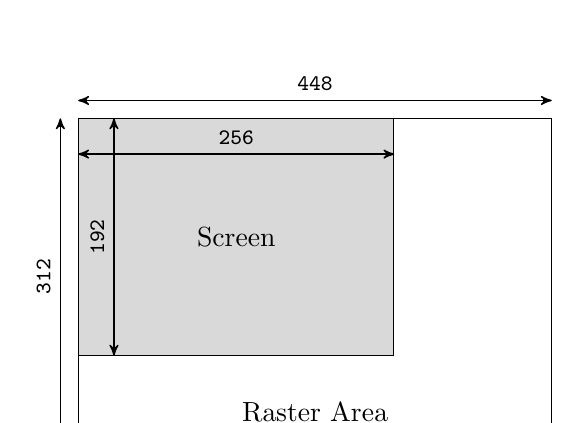
\begin{tikzpicture}[
		baseline=(raster.north),
		framed/.style={draw},
		filled/.style={framed, fill=PrintableLightGray}
	]
		\node[framed, minimum width=6cm, minimum height=4cm, anchor=north west, label={[yshift=1.5em]below:Raster Area}] at(0,0) (raster) {};
		\node[filled, minimum width=4cm, minimum height=3cm, anchor=north west] at(0,0) (screen) {Screen};
	
		\begin{scope}[
			every path/.style={>=stealth', <->, line width=0.5pt},
			every node/.style={font=\footnotesize\ttfamily, midway, above}]
					
			\draw ([yshift=1.5ex]raster.north west) -- ([yshift=1.5ex]raster.north east) node {448};
			\draw ([xshift=-1.5ex]raster.north west) -- ([xshift=-1.5ex]raster.south west) node[rotate=90] {312};
					
			\draw ([yshift=-3ex]screen.north west) -- ([yshift=-3ex]screen.north east) node {256};
			\draw ([xshift=3ex]screen.north west) -- ([xshift=3ex]screen.south west) node[rotate=90] {192};
				
		\end{scope}
	
	\end{tikzpicture}

	&

	The raster area addressable by Copper is 448$\times$312 pixels. So for the standard 256$\times$192 resolution, one horizontal position translates into 8 pixels. The visible portion of the screen is positioned top-left within the raster area like shown in this drawing. This means Copper line 0 corresponds with the top line of the screen, just below the border.

	\\
\end{tabularx}


\subsubsection{HALT}

\begin{BitTableWord}
	\BitMono{1} &
		\BitMono{1} &
		\BitMono{1} &
		\BitMono{1} &
		\BitMono{1} &
		\BitMono{1} &
		\BitMono{1} &
		\BitMono{1} &
	\BitMono{1} &
		\BitMono{1} &
		\BitMono{1} &
		\BitMono{1} &
		\BitMono{1} &
		\BitMono{1} &
		\BitMono{1} &
		\BitMono{1} \\
\end{BitTableWord}

{\tt HALT} is a special case of {\tt WAIT} instruction that tells Copper to wait for the vertical position 511 and horizontal 63. As these are unreachable positions, it will effectively stop all further Copper processing until Next is reset.

% note: we use comma for referencing port declaration page to avoid double closing parenthesis, more readable this way
However, when mode {\tt 11} is used (bits 7-6 of \PortTextXRef[,]{62}), Copper will auto-wrap to the first instruction on every vertical blank. This allows us to use {\tt HALT} to mark the end of the Copper program without having to fill in the remaining bytes with {\tt 0}. Quite convenient! In fact, I'd imagine this would be the most commonly used mode. If you're used to Copper on Amiga, this is also how it behaved there.


\subsubsection{MOVE}

\begin{BitTableWord}
	\BitMono{0} &
	\BitMulti{7}{Next Register ({\tt 0}-{\tt 127})} &
	\BitMulti{8}{Value ({\tt 0}-{\tt 255})} \\
\end{BitTableWord}

{\tt MOVE} writes the given 8-bit value to the given Next register. Any register between {\tt 1} and {\tt 127} (\MemAddr{7F}) can be written to. Register {\tt 0} is a special case, see {\tt NOOP} below.

{\tt MOVE} can be used for all sorts of neat effects. For example: change Layer 2 offsets to achieve parallax scrolling effect, change palette at specific screen coordinates to achieve sky gradient or simulate above and under-water colours etc.


\subsubsection{NOOP}

\begin{BitTableWord}
	\BitMono{0} &
		\BitMono{0} &
		\BitMono{0} &
		\BitMono{0} &
		\BitMono{0} &
		\BitMono{0} &
		\BitMono{0} &
		\BitMono{0} &
	\BitMono{0} &
		\BitMono{0} &
		\BitMono{0} &
		\BitMono{0} &
		\BitMono{0} &
		\BitMono{0} &
		\BitMono{0} &
		\BitMono{0} \\
\end{BitTableWord}

{\tt NOOP} is a special case of {\tt MOVE} that effectively does nothing for a period of one horizontal position. It can be used to fine-tune timing, align colour and display changes etc.


\pagebreak
\subsection{Configuration}
\label{zx_next_copper_configuration}

% note: we only show page number on second port xref since both are declared on the same page, but if this changes in the future, we should update this text accordingly
To load a program, we need to send it, byte by byte, through \PortTextXRef[]{60} or \PortTextXRef[]{63} registers (page \PortPage{60}). As instructions are 16-bits in size, two writes are required. The difference between the two registers is that \MemAddr{60} sends bytes immediately while \MemAddr{63} only after both bytes of an instruction are provided, thus preventing half-written instructions from executing.

% note: we only show page number on second port xref since both are declared on the same page, but if this changes in the future, we should update this text accordingly
Copper is controlled through 16-bit control word accessible through \PortTextXRef[]{62} and \PortTextXRef[]{61} registers (page \PortPage{62}):

\begin{BitTableWord}[c][\PortTextXRef{62}][\PortTextXRef{61}]
	\BitStartMulti{2}{Mode} &
		\BitMono{0} & 
		\BitMono{0} & 
		\BitMono{0} &
		\BitMulti{11}{Index for program upload} \\
\end{BitTableWord}

Mode can be one of the following:

\begin{PortBitConfig}
	\PortBitLine{00}{Stops the Copper, {\tt CPC} keeps its current value. This is useful during program upload, to prevent Copper from executing incomplete instructions and programs.}
	\PortBitLine{01}{Resets {\tt CPC} to {\tt 0}, then starts Copper. From here on, Copper will start executing the first instruction in the program and continue until {\tt CPC} reaches 1023, then wrap around back to first. However it will stop if {\tt HALT} instruction is encountered.}
	\PortBitLine{10}{Starts or resumes Copper from current {\tt CPC}. Similar to {\tt 01}, except that {\tt CPC} is not changed. Instead, Copper resumes execution from current instruction.}
	\PortBitLine{11}{Same as {\tt 01}, but also auto-resets {\tt CPC} to 0 on vertical blank. In this mode we can use {\tt HALT} to mark the end of the program and still repeat it without having to fill-in {\tt NOOP}s from the last instruction of our program to the end of Copper 2K memory.}
\end{PortBitConfig}

% note: we only show page number on second port xref since both are declared on the same page, but if this changes in the future, we should update this text accordingly
The other value we set is the index for program upload. This is 11-bit value ({\tt 0}-{\tt 2047}) specifying the byte offset for write commands with \PortTextXRef[]{60} or \PortTextXRef[]{63} registers (page \PortPage{60}). In other words: this is the index for the location into which data will be uploaded, not the value of the {\tt CPC}. We can't change {\tt CPC} programmatically, apart from resetting it to {\tt 0}.


\subsection{Example}

Enough theory, let's see how it works in practice, Copper program first. It changes palette colour to green at the top of the screen and then to red in the middle:

\begin{tcblisting}{}
CopperList:
	DB &80, 0           ; Wait line 0
	DB &41, %00011100 ; Set palette entry to green
	DB &80, 96          ; Wait line 96
	DB &41, %11100000 ; Set palette entry to red
	DB &FF, &FF         ; HALT
CopperListSize = &-CopperList
\end{tcblisting}

In case you may be wondering: we should also ensure we update the correct colour with \PortTextXRef{43} and \PortTextXRef{40}. But I wanted to keep the program simple for demonstration purposes.

With Copper program in place, we can upload it to Copper memory. We can use DMA or directly upload values through Next registers. The code here demonstrates later, but companion code implements both so you can compare:

\begin{tcblisting}{}
	; Stop Copper and set data upload index to 0
	NEXTREG &61, %00000000
	NEXTREG &62, %00000000

	; Copy list into Copper memory
	LD HL, CopperList           ; HL points to start of copper list
	LD B, CopperListSize        ; B = size of our Copper list in bytes
.nextByte:
	LD A, (HL)                  ; Load current byte to A
	NEXTREG &63, A              ; Copy it to Copper memory
	INC HL                      ; Increment HL to next byte
	DJNZ .nextByte              ; Repeat or continue

	; Start Copper in mode %11 - reset on every vertical blank
	NEXTREG &61, %00000000
	NEXTREG &62, %11000000
\end{tcblisting}

Again, this is an overly simplified example. It only works for lists that are less than 256 bytes long.

The next step is... Well, there is no next step - if we enabled Layer 2 and filled it with the colour we're changing in our Copper list, we should see the screen divided into two halves with top in green and bottom red colour.

Not the most impressive display of Copper capabilities, I give you that. You can find a more complex example in companion code on GitHub, folder {\tt copper} with couple additional points of interest:

\begin{itemize}[topsep=1pt,itemsep=1pt]
	\item Upload routine that supports programs of arbitrary size (within 1024 instructions limit)
	\item Example of upload routine using DMA
	\item Using DMA to fill in Layer 2 banks
	\item Macros that hopefully make Copper programs easier to read and write
	\item Usage of \PortTextXRef{60} to dynamically update individual bytes of the program in memory to achieve couple effects
\end{itemize}


\pagebreak
\subsection{Copper Registers}
\label{zx_next_copper_registers}


\subsubsection{\PortDeclaration{60}}

\begin{NextPort}
	\PortBits{7-0}
		\PortDesc{Data to upload to Copper memory}
\end{NextPort}

% note: port page is not used here since the declaration is on the same page
The data is written to the index specified with \PortTextXRef[]{61} and \PortTextXRef[]{62} registers. After the write, the index is auto-incremented to the next memory position. The index wraps to {\tt 0} when the last byte of the program memory is written to position {\tt 2047}. Since Copper instructions are 16-bits in size, two writes are required to complete each one.


\subsubsection{\PortDeclaration{61}}

\begin{NextPort}
	\PortBits{7-0}
		\PortDesc{Least significant 8 bits of Copper list index}
\end{NextPort}


\subsubsection{\PortDeclaration{62}}

\begin{NextPort}
	\PortBits{7-6}
		\PortDesc{Control mode}
		\PortDescOnly{
			\begin{PortBitConfig}
				\PortBitLine{00}{Stops the Copper, {\tt CPC} keeps its current value}
				\PortBitLine{01}{Resets {\tt CPC} to {\tt 0}, then starts Copper}
				\PortBitLine{10}{Starts or resumes Copper from current {\tt CPC}}
				\PortBitLine{11}{Same as {\tt 01}, but also auto-resets {\tt CPC} to 0 on vertical blank}
			\end{PortBitConfig}
		}
	\PortBits{5-3}
		\PortDesc{Reserved, must be {\tt 0}}
	\PortBits{2-0}
		\PortDesc{Most significant 3 bits of Copper list index}
\end{NextPort}

When control mode is identical to current one, it's ignored. This allows change of the upload index without restarting the program.


\subsubsection{\PortDeclaration{63}}

\begin{NextPort}
	\PortBits{7-0}
		\PortDesc{Data to upload to Copper memory}
\end{NextPort}

% note: port page is not used here since the declaration is on the same page
Similar to \PortTextXRef[]{60} except that writes are only committed to Copper memory after two bytes are written. This prevents half-written instructions to be executed.

The first write to this register is for MSB of the Copper instruction or even instruction address and second write for LSB or odd instruction address.


\pagebreak
\IntentionallyEmpty
\pagebreak

	\section{Sound}
\label{zx_next_sound}

% ────────────────────────────────────────────────────────────────────────────────────
% ─██████████████─██████████████─██████──██████─██████──────────██████─████████████───
% ─██░░░░░░░░░░██─██░░░░░░░░░░██─██░░██──██░░██─██░░██████████──██░░██─██░░░░░░░░████─
% ─██░░██████████─██░░██████░░██─██░░██──██░░██─██░░░░░░░░░░██──██░░██─██░░████░░░░██─
% ─██░░██─────────██░░██──██░░██─██░░██──██░░██─██░░██████░░██──██░░██─██░░██──██░░██─
% ─██░░██████████─██░░██──██░░██─██░░██──██░░██─██░░██──██░░██──██░░██─██░░██──██░░██─
% ─██░░░░░░░░░░██─██░░██──██░░██─██░░██──██░░██─██░░██──██░░██──██░░██─██░░██──██░░██─
% ─██████████░░██─██░░██──██░░██─██░░██──██░░██─██░░██──██░░██──██░░██─██░░██──██░░██─
% ─────────██░░██─██░░██──██░░██─██░░██──██░░██─██░░██──██░░██████░░██─██░░██──██░░██─
% ─██████████░░██─██░░██████░░██─██░░██████░░██─██░░██──██░░░░░░░░░░██─██░░████░░░░██─
% ─██░░░░░░░░░░██─██░░░░░░░░░░██─██░░░░░░░░░░██─██░░██──██████████░░██─██░░░░░░░░████─
% ─██████████████─██████████████─██████████████─██████──────────██████─████████████───
% ────────────────────────────────────────────────────────────────────────────────────

Next inherits the same 3 AY-3-8912 chips setup as used in 128K Spectrums. This allows us to reuse many of the pre-existing applications and routines to play sound effects and music.

\subsection{AY Chip Registers}

AY chip has 3 sound channels, called A, B and C. Combined with 3 chips, this allows us to produce 9 channel music. Programming wise, each of the 3 chips needs to be selected first via \PortTextXRef{FFFD} register. Afterwards, we can set various parameters through \PortTextXRef{08} and \PortTextXRef{09} registers.

AY chip is controlled by 14 internal registers. To program them, we first need to select the register with \PortTextXRef{FFFD} and then write the value with \PortTextXRef{BFFD}.


\subsection{Editing and Players}

Several applications can produce sounds or music compatible with the AY chip. For sounds, Shiru's AYFX Player\footnote{\url{https://shiru.untergrund.net/software.shtml\#old}} can be used. This program also includes a Z80 native player that can directly load and play sound effects. Alternatively, Remy's AY audio generator website\footnote{\url{https://zx.remysharp.com/audio/}} can produce exactly the same results and is fully compatible with AYFX Player.

A different way of playing sounds is to convert the WAV file into 1, 2 or 4-bit per sample sound with the ChibiWave application. Sounds take a bit more memory this way but are much easier to create. You can find the application, as well as tutorial and playback source code on Chibi Akumas website\footnote{\url{https://www.chibiakumas.com/z80/platform4.php\#LessonP35}}. While there, definitely check other tutorials too - they're all high quality and available as both, written posts and YouTube videos.

For creating music there are also several options. NextDAW\footnote{\url{https://nextdaw.biasillo.com/}} is native composer that runs on ZX Spectrum Next itself. Or if you prefer cross-platform, Arkos Tracker\footnote{\url{https://www.julien-nevo.com/arkostracker/}} or Vortex Tracker\footnote{\url{https://bulba.untergrund.net/vortex_e.htm}} should do the job. All include ``drivers''; Z80 code you can include in your program that can load and play created music.


\pagebreak
\subsection{Examples}

Before we can start playing sounds, we need to enable the sound hardware. While this is usually enabled by default, it's nonetheless a good idea to ensure our program will always run under the same conditions.

\begin{tcblisting}{}
	; Setup Turbo Sound chip
	LD BC, &FFFD            ; Turbo Sound Next Control Register
	LD A, %11111101         ; Enable left+right audio, select AY1
	OUT (C), A
	
	; Setup mapping of chip channels to stereo channels
	NEXTREG &08, %00010010  ; Use ABC, enable internal speaker & turbosound
	NEXTREG &09, %11100000  ; Enable mono for AY1-3
\end{tcblisting}

Programming AY consists of writing various values to its registers. As mentioned, this is a two-step process: first select register number, then write the value. Multiple writes are required for each tone to set period, volume etc. To make it simpler, I created a subroutine. It takes 2 parameters: {\tt A} for register number ({\tt 0-13}) and {\tt D} with value to write.

\begin{tcblisting}{}
WriteDToAYReg:
	; Select desired register
	LD BC, &FFFD
	OUT (C), A
	
	; Write given value
	LD A, D
	LD BC, &BFFD
	OUT (C), A
	
	RET
\end{tcblisting}

Companion code on GitHub, folder {\tt sound} includes expanded code as well as a simple player that plays multiple tones in sequence. For the purposes of this book, I used Remy's AY audio generator website to load one of the example effects, then manually copied raw values into the source code. Laborious process to say the least - this is not how effects should be handled in real life. But I wanted to learn and demonstrate how to program AY chip, not how to use ready-made drivers to play effects or music. Furthermore, my ``player'' blocks the main loop; ideally, sound effects and music would play on the interrupt handler. This could be a nice homework for the reader - example in section \XRef{zx_next_interrupts} should give you an idea of how to achieve this - happy coding!


\pagebreak
\subsection{Sound Ports and Registers}
\label{zx_next_sound_registers}

\subsubsection{\PortDeclaration{FFFD}}

When bit {\tt 7} is {\tt 1}:

\begin{NextPort}
	\PortBits{7}
		\PortDesc{{\tt 1}}
	\PortBits{6}
		\PortDesc{{\tt 1} to enable left audio}
	\PortBits{5}
		\PortDesc{{\tt 1} to enable right audio}
	\PortBits{4-2}
		\PortDesc{Must be {\tt 1}}
	\PortBits{1-0}
		\PortDesc{Selects active chip:}
		\PortDescOnly{
			\begin{PortBitConfig}
				\PortBitLine{00}{Unused}
				\PortBitLine{01}{AY3}
				\PortBitLine{10}{AY2}
				\PortBitLine{11}{AY1}
			\end{PortBitConfig}
		}
\end{NextPort}

When bit {\tt 7} is {\tt 0}:

\begin{NextPort}
	\PortBits{7}
		\PortDesc{{\tt 0}}
	\PortBits{6-0}
		\PortDesc{Selects given AY register number for read or write from active sound chip} 
\end{NextPort}


\subsubsection{\PortDeclaration{BFFD}}

\begin{NextPort}
	\PortBits{7-0}
		\PortDesc{Writes given value to currently selected register:}
\end{NextPort}

\begingroup
	\small
	\vspace*{8pt}					% some vertical spacing between port table and this sectino
	\setlength{\leftskip}{1.25cm}	% Setup left margin as if this whole section was within port table (tried adding it there but got syntax errors)

	\newcommand{\AYRegTitle}[1]{
		\subsubsection{#1}
		\vspace*{-1ex}
	}

	\begin{multicols}{2}
		\AYRegTitle{0 - Channel A tone, low byte}
		\begin{BitTableByte}
			\BitStartMulti{8}{A tone} \\
		\end{BitTableByte}
		
		\AYRegTitle{1 - Channel A tone, high 4-bits}
		\begin{BitTableByte}
			\BitMono{0} & \BitMono{0} & \BitMono{0} & \BitMono{0} & \BitMulti{4}{A tone high} \\
		\end{BitTableByte}		
	\end{multicols}

	\begin{multicols}{2}
		\AYRegTitle{2 - Channel B tone, low byte}
		\begin{BitTableByte}
			\BitStartMulti{8}{B tone} \\
		\end{BitTableByte}

		\AYRegTitle{3 - Channel B tone, high 4-bits}
		\begin{BitTableByte}
			\BitMono{0} & \BitMono{0} & \BitMono{0} & \BitMono{0} & \BitMulti{4}{B tone high} \\
		\end{BitTableByte}
	\end{multicols}

	\begin{multicols}{2}
		\AYRegTitle{4 - Channel C tone, low byte}
		\begin{BitTableByte}
			\BitStartMulti{8}{C tone} \\
		\end{BitTableByte}

		\AYRegTitle{5 - Channel C tone, high 4-bits}
		\begin{BitTableByte}
			\BitMono{0} & \BitMono{0} & \BitMono{0} & \BitMono{0} & \BitMulti{4}{C tone high} \\
		\end{BitTableByte}
	\end{multicols}

	\pagebreak
	\begin{multicols}{2}
		\AYRegTitle{6 - Noise period}
		\begin{BitTableByte}
			\BitMono{0} & \BitMono{0} & \BitMono{0} & \BitMulti{5}{Noise Period} \\
		\end{BitTableByte}
		\leavevmode	% for some reason new line \\ doesn't work here with BitTableByte/ElegantTable

		\columnbreak

		\AYRegTitle{7 - Flags}
		\begin{BitTableByte}
			\BitMono{0} & \BitMono{0} & \BitMono{C} & \BitMono{B} & \BitMono{A} & \BitMono{C} & \BitMono{B} & \BitMono{A} \\
			\hline
			\BitMono{0} & \BitMono{0} & \BitMulti{3}{Noise} & \BitMulti{3}{Tone} \\
		\end{BitTableByte}
	\end{multicols}

	\begin{multicols}{2}
		\AYRegTitle{8 - Channel A volume/envelope}
		\begin{BitTableByte}
			\BitMono{0} & \BitMono{0} & \BitMono{0} & \BitMono{0} & \BitMulti{4}{A Volume} \\
		\end{BitTableByte}

		\AYRegTitle{9 - Channel B volume/envelope}
		\begin{BitTableByte}
			\BitMono{0} & \BitMono{0} & \BitMono{0} & \BitMono{0} & \BitMulti{4}{B Volume} \\
		\end{BitTableByte}
	\end{multicols}

	\begin{multicols}{2}
		\AYRegTitle{10 - Channel C volume/envelope}
		\begin{BitTableByte}
			\BitMono{0} & \BitMono{0} & \BitMono{0} & \BitMono{0} & \BitMulti{4}{C Volume} \\
		\end{BitTableByte}

		\columnbreak

		\textbf{Note:} Registers {\tt 8-10} work as volume control if bit {\tt 4} is {\tt 0}, otherwise envelop generator is
		used (see registers {\tt 11-13}). In this case bits {\tt 3-0} are ignored.
	\end{multicols}

	\begin{multicols}{2}
		\AYRegTitle{11 - Envelope period fine}
		\begin{BitTableByte}
			\BitStartMulti{8}{Envelope bits 7-0} \\
		\end{BitTableByte}

		\AYRegTitle{12 - Envelope period coarse}
		\begin{BitTableByte}
			\BitStartMulti{8}{Envelope bits 15-8} \\
		\end{BitTableByte}
	\end{multicols}

	\begin{multicols}{2}
		\AYRegTitle{13 - Envelope shape}
		\begin{BitTableByte}
			\BitMono{0} & \BitMono{0} & \BitMono{0} & \BitMono{0} & \BitMono{$C$} & \BitMono{$A_t$} & \BitMono{$A_l$} & \BitMono{$H$} \\
		\end{BitTableByte}
	\end{multicols}

	\hspace*{1.3cm}
	\begin{tabular}{lllp{18cm}}
		$H$ & \multicolumn{3}{l}{``Hold''} \\
			& {\tt 1} & \multicolumn{2}{p{10cm}}{envelope generator performs 1 cycle then holds the end value} \\
			& {\tt 0} & \multicolumn{2}{p{10cm}}{cycles continuously} \\

		$A_l$ & \multicolumn{3}{l}{``Alternate''} \\
			& \multicolumn{3}{l}{If ``hold'' set} \\
			& & {\tt 1} & the value held is initial value \\
			& & {\tt 0} & the value held is the final value \\
			& \multicolumn{3}{l}{If ``hold'' not set} \\
			& & {\tt 1} & envelope generator alters direction after each cycle \\
			& & {\tt 0} & resets after each cycle \\

		$A_t$ & \multicolumn{3}{l}{``Attack''} \\
			& {\tt 1} & \multicolumn{2}{l}{the generator counts up} \\
			& {\tt 0} & \multicolumn{2}{l}{the generator counts down} \\

		$C$ & \multicolumn{3}{l}{``Continue''} \\
			& {\tt 1} & \multicolumn{2}{l}{``hold'' is followed} \\
			& {\tt 0} & \multicolumn{2}{p{12cm}}{the envelope generator performs one cycle then drops volume to 0 and stays there, overriding ``hold''} \\
	\end{tabular}
\endgroup

\subsubsection{\PortDeclaration{06}}

\begin{NextPort}
	\PortBits{7}
		\PortDesc{{\tt 1} to enable CPU speed mode key "F8", {\tt 0} to disable ({\tt 1} after soft reset)}
	\PortBits{6}
		\PortDesc{Core 3.1.2+: Divert BEEP-only to internal speaker ({\tt 0} after hard reset)}
		\PortDescOnly{Pre core 3.1.2: DMA mode, {\tt 0} zxnDMA, {\tt 1} Z80 DMA ({\tt 0} after hard reset)}
	\PortBits{5}
		\PortDesc{Core 2.0+: {\tt 1} to enable "F3" key (50/60 Hz switch) ({\tt 1} after soft reset)}
		\PortDescOnly{Pre core 2.0: "Enable Lightpen"}
	\PortBits{4}
		\PortDesc{{\tt 1} to enable DivMMC automap and DivMMC NMI by DRIVE button ({\tt 0} after hard reset)}
	\PortBits{3}
		\PortDesc{{\tt 1} to enable multiface NMI by M1 button ({\tt 0} after hard reset)}
	\PortBits{2}
		\PortDesc{{\tt 1} to set primary device to mouse in PS/2 mode, {\tt 0} to set to keyboard}
	\PortBits{1-0}
		\PortDesc{Audio chip mode:}
		\PortDescOnly{
			\begin{PortBitConfig}
				\PortBitLine{00}{YM}				
				\PortBitLine{01}{AY}
				\PortBitLine{10}{Disabled}
				\PortBitLine{11}{Core 3.0+: Hold all AY in reset}
			\end{PortBitConfig}
		}
\end{NextPort}

\subsubsection{\PortDeclaration{08}}

\begin{NextPort}
	\PortBits{7}
		\PortDesc{{\tt 1} unlock / {\tt 0} lock port \PortTextXRef{7FFD} paging}
	\PortBits{6}
		\PortDesc{{\tt 1} to disable RAM and I/O port contention ({\tt 0} after soft reset)}
	\PortBits{5}
		\PortDesc{AY stereo mode ({\tt 0} = ABC, {\tt 1} = ACB) ({\tt 0} after hard reset)}
	\PortBits{4}
		\PortDesc{Enable internal speaker ({\tt 1} after hard reset)}
	\PortBits{3}
		\PortDesc{Enable 8-bit DACs (A,B,C,D) ({\tt 0} after hard reset)}
	\PortBits{2}
		\PortDesc{Enable port \MemAddr{FF} Timex video mode read ({\tt 0} after hard reset)}
	\PortBits{1}
		\PortDesc{Enable Turbosound (currently selected AY is frozen when disabled) ({\tt 0} after hard reset)}
	\PortBits{0}
		\PortDesc{Implement Issue 2 keyboard (port \MemAddr{FE} reads as early ZX boards) ({\tt 0} after hard reset)}
\end{NextPort}

\subsubsection{\PortTextXRef[]{09}}

\PortDeclarationXRef{Sprites}{09}


\pagebreak
\IntentionallyEmpty
\pagebreak

	\section{Keyboard}
\label{zx_next_keyboard}

% ───────────────────────────────────────────────────────────────────
% ─██████──████████─██████████████─████████──████████─██████████████─
% ─██░░██──██░░░░██─██░░░░░░░░░░██─██░░░░██──██░░░░██─██░░░░░░░░░░██─
% ─██░░██──██░░████─██░░██████████─████░░██──██░░████─██░░██████████─
% ─██░░██──██░░██───██░░██───────────██░░░░██░░░░██───██░░██─────────
% ─██░░██████░░██───██░░██████████───████░░░░░░████───██░░██████████─
% ─██░░░░░░░░░░██───██░░░░░░░░░░██─────████░░████─────██░░░░░░░░░░██─
% ─██░░██████░░██───██░░██████████───────██░░██───────██████████░░██─
% ─██░░██──██░░██───██░░██───────────────██░░██───────────────██░░██─
% ─██░░██──██░░████─██░░██████████───────██░░██───────██████████░░██─
% ─██░░██──██░░░░██─██░░░░░░░░░░██───────██░░██───────██░░░░░░░░░░██─
% ─██████──████████─██████████████───────██████───────██████████████─
% ───────────────────────────────────────────────────────────────────

Next inherits ZX Spectrum keyboard handling, so all legacy programs will work out of the box. Additionally, it allows reading the status of extended keys.


\subsection{Legacy Keyboard Status}

ZX Spectrum uses 8$\times$5 matrix for reading keyboard status. This means 40 distinct keys can be represented. The keyboard is read from \PortTextXRef{xxFE} with particular high bytes. There are 8 possible bytes, each will return the status of 5 associated keys. If a key is pressed, the corresponding bit is set to {\tt 0} and vice versa.

Example for checking if {\tt P} or {\tt I} is pressed:
	
\begin{tcblisting}{}
    LD BC, &DFFE     ; We want to read keys..... YUIOP
    IN A, (C)        ; A holds values in bits... 43210
checkP:
    BIT 0, A         ; test bit 0 of A (P key)
    JR NZ checkI     ; if bit0=1, P not pressed
    ...              ; P is pressed
checkI:
    BIT 2, A         ; test bit 2 of A (I key)
    JR NZ continue   ; if bit2=1, I not pressed
    ...              ; I is pressed
continue:
\end{tcblisting}

As mentioned in Ports chapter, section \XRef{zx_next_ports_examples}, we can slightly improve performance if we replace first two lines with:

\begin{tcblisting}{}
    LD A, &DF
    IN (&FE)
\end{tcblisting}

Reading the port in first example requires 22 t-states (10+12) vs. 18 (7+11). The difference is small, but it can add up as typically keyboard is read multiple times per frame.

The first program is more understandable at a glance - the port address is given as a whole 16-bit value, as usually provided in the documentation. The second program splits it into 2 8-bit values, so intent may not be immediately apparent. Of course, one learns the patterns with experience, but it nonetheless demonstrates the compromise between readability and speed.


\subsection{Next Extended Keys}

% note: we only show page number after last port xref since both are declared on the same page, but if this changes in the future, we should update this text accordingly
Next uses larger 8$\times$7 matrix for keyboard, with 10 additional keys. By default, hardware is translating keys from extra two columns into the existing 8$\times$5 set. But you can turn this off with bit {\tt 4} of \PortTextXRef{68}. Extra keys can be read separately via \PortTextXRef[]{B0} and \PortTextXRef[]{B1}, details on page \PortPage{B0}.


\subsection{Keyboard Ports and Registers}
\label{zx_next_keyboard_registers}

\subsubsection{\PortDeclaration{xxFE}}

\vspace*{-1em} % for some reason LaTeX adds some unwanted vertical space between title and text!?
Returns keyboard status when read with certain high byte values:

{
	\tt
	\setlength{\extrarowheight}{0pt}
	\def\arraystretch{0.1}
	
	\begin{tabular}{p{0.7cm}|cp{1cm}p{1cm}p{1cm}p{1.3cm}p{1.5cm}}

		~xx & & 4 & 3 & 2 & 1 & 0 \instrb \\
		\hline
		\MemAddr{7F}\instrt & & B & N & M & Symb & Space \\
		\MemAddr{BF}\instrt & & H & J & K & L & Enter \\
		\MemAddr{DF}\instrt & & Y & U & I & O & P \\
		\MemAddr{EF}\instrt & & 6 & 7 & 8 & 9 & 0 \\
		\MemAddr{F7}\instrt & & 5 & 4 & 3 & 2 & 1 \\
		\MemAddr{FB}\instrt & & T & R & E & W & Q \\
		\MemAddr{FD}\instrt & & G & F & D & S & A \\
		\MemAddr{FE}\instrt\instrb & & V & C & X & Z & Caps \\

	\end{tabular}
}

Bits are reversed: if a key is pressed, the corresponding bit is {\tt 0}, if a key is not pressed, bit is {\tt 1}.

% note: we don't show page next to port since we use more verbose link to the section+page afterwards
Note: when written to, \PortTextXRef[]{xxFEWrite} is used to set border colour and audio devices. See ULA Layer, section \PortXRef{xxFEWrite} for details.


\subsubsection{\PortTextXRef[]{68}}

\PortDeclarationXRef{Tilemap}{68}


\subsubsection{\PortDeclaration{B0}}
\vspace*{-2ex}
\subsubsection{\PortDeclaration{B1}}

\newcommand{\PortNextExtKey}[2]{{\tt 0} if key pressed, {\tt 1} otherwise & {\tt #1} & {\tt #2} \\ }
\begin{NextPort}[cp{5.5cm}p{1.5cm}X][Bit & Effect & \MemAddr{B0} & \MemAddr{B1}]
	\PortBits{7}
		\PortNextExtKey{;}{Delete}
	\PortBits{6}
		\PortNextExtKey{"}{Edit}
	\PortBits{5}
		\PortNextExtKey{,}{Break}
	\PortBits{4}
		\PortNextExtKey{.}{Inv Video}
	\PortBits{3}
		\PortNextExtKey{Up}{True Video}
	\PortBits{2}
		\PortNextExtKey{Down}{Graph}
	\PortBits{1}
		\PortNextExtKey{Left}{Caps Lock}
	\PortBits{0}
		\PortNextExtKey{Right}{Extend}
\end{NextPort}

Available since core 3.1.5

\pagebreak
	\section{Interrupts on Next}
\label{zx_next_interrupts}

% ─────────────────────────────────────────────────────────────────────
% ─██████████─██████──────────██████─██████████████─████████████████───
% ─██░░░░░░██─██░░██████████──██░░██─██░░░░░░░░░░██─██░░░░░░░░░░░░██───
% ─████░░████─██░░░░░░░░░░██──██░░██─██████░░██████─██░░████████░░██───
% ───██░░██───██░░██████░░██──██░░██─────██░░██─────██░░██────██░░██───
% ───██░░██───██░░██──██░░██──██░░██─────██░░██─────██░░████████░░██───
% ───██░░██───██░░██──██░░██──██░░██─────██░░██─────██░░░░░░░░░░░░██───
% ───██░░██───██░░██──██░░██──██░░██─────██░░██─────██░░██████░░████───
% ───██░░██───██░░██──██░░██████░░██─────██░░██─────██░░██──██░░██─────
% ─████░░████─██░░██──██░░░░░░░░░░██─────██░░██─────██░░██──██░░██████─
% ─██░░░░░░██─██░░██──██████████░░██─────██░░██─────██░░██──██░░░░░░██─
% ─██████████─██████──────────██████─────██████─────██████──██████████─
% ─────────────────────────────────────────────────────────────────────

Like many other functionalities, Next also inherits interrupts handling from ZX Spectrum. As described in the Z80 chapter, section \XRef{z80_interrupts}, Interrupt Mode 0 is used for a short period of time after booting up, before ROM activates Mode 1. IM1 remains active unless we explicitly change it. To replace the default IM1 interrupt handler, we can page out ROM or change to Interrupt Mode 2.

% note: we reference page number manually since both registers are declared on the same page, but if this changes in the future, we should update this text accordingly
Both IM1 and IM2 are triggered by standard Spectrum ULA on every video frame. However timing can be adjusted using \PortTextXRef[]{22} and \PortTextXRef[]{23} registers (page \PortPage{22}). This allows disabling standard ULA interrupt, or add an extra interrupt that occurs on a particular video line.

Interrupts are most frequently used for driving music playback. Though they can also be used for other purposes such as synchronizing game state etc.


\subsection{Interrupt Mode 1}

In Interrupt Mode 1, an interrupt handler is expected on address \MemAddr{0038} in ROM. Default handler updates frame counter system variable, scans the keyboard and updates keyboard state system variables. We can replace it with our routine by paging out ROM.

Let's see how to do this with an example. We will use the interrupt routine to update an 8-bit counter. The example uses {\tt sjasmplus} directives to establish paging. If you are using a different assembler, you may need to change! First, let's prepare the groundwork - declare the variable and main part of the program:

\begin{tcblisting}{}
    DEVICE ZXSPECTRUMNEXT ; this is Next program - important for paging setup!

    ORG &8000              ; set PC to &8000
Start:
    DI                     ; disable interrupts while we page out ROM
    NEXTREG &50, 28        ; page out ROM in slot 0 (&000-&1FFF) with page 28
    IM 1                   ; enable Interrupt Mode 1
    EI                     ; enable interrupts

.loop:
    JP .loop               ; infinite loop
    RET                    ; this is never reached...

counter: DB 0              ; counter variable
\end{tcblisting}

The first directive tells {\tt sjasmplus} to generate the code for Next. This will become important later on. Then we set the program counter to \MemAddr{8000}; all subsequent instructions and data will be assembled starting at this address.

Next, we are paging out ROM in 8K slot 0 with bank 28. We'll write our interrupt handler subroutine into this bank later on. Afterwards, we enable Interrupt Mode 1. This is optional; by default, Next will run in this mode already, but being explicit is more future proof. Maybe another program would change to IM2. Note how we disable interrupts during this setup to prevent undesired side effects.

The remaining part is simply an infinite loop to prevent the program from exiting. And finally, we declare our counter variable.

The interrupt subroutine is expected at \MemAddr{0038}. There are several ways to achieve this with {\tt sjasmplus}. I opted for explicit slot/bank technique so we're in control of the paging:

\begin{tcblisting}{}
    SLOT 6             ; activate slot 6
    PAGE 28            ; load page 28K to active slot
    ORG &C038          ; set PC to &C038

InterruptHandler:
    LD HL, counter     ; load address of counter var
    INC (HL)           ; increment it
    EI                 ; enable interrupts
    RETI               ; return from interrupt
\end{tcblisting}

This is where the previously mentioned {\tt DEVICE} directive comes to play - {\tt sjasmplus} decides slot and bank configuration based on it. {\tt ZXSPECTRUMNEXT} assumes 8K slot and bank size. Lines 1-3 are the key to ensure our interrupt handler will be present on \MemAddr{0038}:

\begin{itemize}
	\item {\tt SLOT} directive tells {\tt sjasmplus} we want the following section to be loaded into 8K slot 6, addresses \MemAddr{C000}-\MemAddr{DFFF}.
	
	\item Next, we specify 8K bank number to load into the selected slot with {\tt PAGE} directive. Subsequent code will be assembled into this bank. This step is optional; default bank would be used otherwise, 0 in this case (see section \XRef{zx_next_memorypaging}). Being explicit is more future proof though. I chose bank 28 but feel free to use others. What's important is to use the same bank with {\tt NEXTREG} instruction when paging out ROM!
	
	\item Since we selected slot 6, we also need to set the program counter to the corresponding address - we want the code to be assembled into the selected bank that we will page into ROM slot 0 at runtime. Because interrupt handler is expected on \MemAddr{0038}, we need to start at \MemAddr{C038} (slot 6 starts at \MemAddr{C000}, but this will be loaded into slot 0 at \MemAddr{0000}).
\end{itemize}

Not that hard, right!? It may take a while to wrap the head around those {\tt SLOT}, {\tt PAGE} and {\tt ORG} directives and addresses, but it's quite straightforward otherwise. While at it: this same technique can be used to load assets into specific banks and then page them in during runtime!

You can find the full source code for this example in companion code, folder {\tt im1}. Feel free to run it, set breakpoints and see how the counter is being changed.

Note there's one potentially deal-breaking issue with this approach: since we are paging out ROM, we can't use any of its functionality. For example, ROM routines like print text at \MemAddr{203C}. But we can do this with IM2 - read on!


\subsection{Interrupt Mode 2}

Once Interrupt Mode 2 is activated, mode 1 handler at \MemAddr{0038} isn't called anymore. Instead, when an interrupt occurs, Z80 performs the following steps:

\begin{itemize}[topsep=1pt,itemsep=1pt]
	\item First, a 16-bit address is formed where the value for the most significant byte is taken from the {\tt I} register and the value for the least significant byte from the current value of the data bus.
	
	\item Two bytes are read from this address (little endian format is assumed - low byte first, then high byte); these 2 bytes form another 16-bit address.
	
	\item It's this second address that the CPU treats as an interrupt routine and starts executing from.
\end{itemize}

\vspace*{1ex}
\begin{tabularx}{\linewidth}{p{6cm}X}
	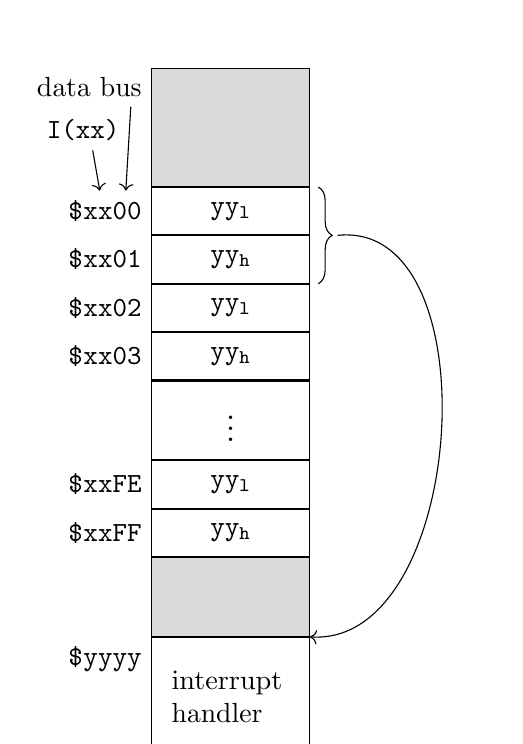
\begin{tikzpicture}[
		baseline=(bus.base),
		framed/.style={draw, font=\ttfamily, minimum width=2cm, minimum height=0.6cm},
		filled/.style={framed, fill=PrintableLightGray}
	]
		
		\node[filled, minimum height=1.5cm] (contentstart) {};
		\node[framed, below=0pt of contentstart] (contentxx00) {yy\Low};
		\node[framed, below=0pt of contentxx00] (contentxx01) {yy\High};
		\node[framed, below=0pt of contentxx01] (contentxx02) {yy\Low};
		\node[framed, below=0pt of contentxx02] (contentxx03) {yy\High};
		\node[framed, minimum height=1cm, below=0pt of contentxx03] (contentxx04) {\vdots};
		\node[framed, below=0pt of contentxx04] (contentxxfe) {yy\Low};
		\node[framed, below=0pt of contentxxfe] (contentxxff) {yy\High};
		\node[filled, minimum height=1cm, below=0pt of contentxxff] (contentmiddle) {};
		\node[framed, minimum height=1.5cm, text width=1.5cm, below=0pt of contentmiddle] (contentyyyy) {\rmfamily interrupt handler};
			
		\node[left=0pt of contentstart.north west, anchor=north east] (bus) {data bus};
		\node[left=8pt of contentstart.north west, anchor=north east, yshift=-15pt] (I) {\tt I(xx)};
			
		\node[left=0pt of contentxx00] (memxx00) {\MemAddr{xx00}};
		\node[left=0pt of contentxx01] (memxx01) {\MemAddr{xx01}};
		\node[left=0pt of contentxx02] (memxx02) {\MemAddr{xx02}};
		\node[left=0pt of contentxx03] (memxx03) {\MemAddr{xx03}};
		\node[left=0pt of contentxxfe] (memxxfe) {\MemAddr{xxFE}};
		\node[left=0pt of contentxxff] (memxxff) {\MemAddr{xxFF}};
		\node[left=0pt of contentyyyy.north west, anchor=north east] (memyyyy) {\MemAddr{yyyy}};
			
		\draw[decorate,decoration={brace,amplitude=5pt,raise=3pt},yshift=0pt]
			(contentxx00.north east) -- (contentxx01.south east)
			node[midway,xshift=1.5ex] (yyyyaddress) {};
		
		\path[->, bend left, out=100, in=90] (yyyyaddress.east) edge (contentyyyy.north east);
			
		\path[->, draw] (I.295) -- (memxx00.105);
		\path[->, draw] (bus.335) -- (memxx00.45);
		
	\end{tikzpicture}

	&

	\vspace*{-1em}

	% paragraphs don't work within tabular, so we use left aligned description instead...
	\begin{description}[topsep=0pt,itemsep=1pt,labelindent=-1.25ex,leftmargin=0cm]
		\item In other words:
		
		\item Because the LSB for the vector table address is effectively a random number, we need to allocate 256 bytes in the memory, on 256-byte boundary (meaning any address with low byte \MemAddr{00} - \MemAddr{xx00}). This gives us a chunk of memory where low byte starts at \MemAddr{00} up to \MemAddr{FF}, thus covering all possible 8-bit values the data bus can ``throw'' at us. This chunk, called ``vector table'', is 256 bytes long and consists of 128 16-bit addresses (vectors), all pointing to the IM2 interrupt handler routine.
		
		\item We are responsible for assigning the high byte of the vector table address to {\tt I} register though. Together 16-bit address for vector table lookup looks like this:
	\end{description}
	
	\vspace*{1ex}

	{ % tabularx requires inner table to be embedded within curlies...
	\begin{ElegantTable}{|C{3cm}|C{3cm}|}
		\ElegantHeader{\EH{15-8} & \EH{7-0}}

		\rowcolor{PrintableBackground} % not sure why header colour is spilled over the whole table in this instance!?
		{\tt I} register & Data Bus \\
	\end{ElegantTable}
	}

	\\
\end{tabularx}

Phew, a lot of words and concepts to grasp. But it's simpler than it sounds - let's rewrite the IM1 example, but this time with IM2. The main program first:

\begin{tcblisting}{}
    ORG &8000              ; set PC to &8000
Start:
    DI                     ; disable interrupts while we setup interrupts
    CALL SetupInterruptVectors
    IM 2                   ; enable Interrupt Mode 2
    EI                     ; enable interrupts
    |(the rest is the same as in IM1 example)|
\end{tcblisting}

Almost the same except for the {\tt NEXTREG} replaced with {\tt SetupInterruptVectors} subroutine call that initializes vector table:

\begin{tcblisting}{}
SetupInterruptVectors:
    LD DE, InterruptHandler        ; prepare pointer to IM2 routine
    LD HL, InterruptVectorTable   ; prepare pointer to vector table
    LD B, 128                      ; we need to fill 128 addresses
.loop:
    LD (HL), E                     ; copy low byte
    INC HL                         ; increment vector table pointer
    LD (HL), D                     ; copy high byte
    INC HL                         ; increment vector table pointer
    DJNZ .loop                     ; repeat until the end of the vector table
    LD A, InterruptVectorTable >> 8
    LD I, A                        ; I now holds high byte of vector table
    RET
\end{tcblisting}

The subroutine fills in all 128 entries of the vector table with the address of our actual interrupt routine. The only remaining piece is the declaration of the vector table itself; I chose {\tt .ALIGN 256} directive that fills in bytes until 256-byte boundary is reached:

\begin{tcblisting}{}
    .ALIGN 256                     ; section must start on 256-byte boundary &xx00
InterruptVectorTable:              ; I register should therefore have value &xx
    DEFS 128*2                     ; 128 16-bit vectors	
\end{tcblisting}

The interrupt handler itself can reside anywhere in the memory. Code-wise it's the same as for IM1 mode previously.

So there's some more work when using IM2 mode, but it leaves ROM untouched so we can rely on its routines and other functionality. I only demonstrated relevant bits here. You can find a fully working example in companion code, folder {\tt im2} (make sure to \textbf{read the next section}!).


\subsubsection{What About Odd Data Bus Values?}

Sharp-eyed readers may be wondering what would happen if the value from the data bus is odd? Given our IM2 example from above, our interrupt handler happens to be on address \MemAddr{802A}. Therefore the vector table would have the following contents:

\begin{ElegantTable}{|c|c|c|c|C{3cm}|c|c|}
	\ElegantHeader{\MemAddr{xx00} & \MemAddr{xx01} & \MemAddr{xx02} & \MemAddr{xx03} & ... & \MemAddr{xxFE} & \MemAddr{xxFF}}

	\MemAddr{2A} & \MemAddr{80} & \MemAddr{2A} & \MemAddr{80} & ... & \MemAddr{2A} & \MemAddr{80} \\
\end{ElegantTable}

If the bus value is even, for example {\tt 0}, {\tt 2}, {\tt 4} etc, then the address of the interrupt handler would be correctly read as \MemAddr{802A} (remember, Z80 is little-endian). But what if the value is odd, {\tt 1}, {\tt 3}, {\tt 5} etc? In this case, 16-bit interrupt handler address would be wrong - \MemAddr{2A80}! During my tests, this didn't happen - whether by luck, the data bus always had an even number, or, maybe Z80 reset bit 0 before constructing vector lookup address. But we can't rely on luck!

In fact, Next Dev Wiki\footnote{\url{https://wiki.specnext.dev/Interrupts}} recommends that the interrupt handler routine is always placed on an address where high and low bytes are equal. It's best to follow this advice to avoid potential issues. The changes to the code are minimal, so I won't show it here - it could be a nice exercise though! Just a tip - to be extra safe, make vector table 257 bytes long in case the data bus has \MemAddr{FF}. You can find a working example in companion code, folder {\tt im2safe}.


\subsection{Hardware Interrupt Mode 2}

In addition to regular IM2, Next also supports a ``Hardware IM2'' mode. This mode works similar to legacy IM2 in that we still need to provide vector tables. But it properly implements the Z80 IM2 scheme with daisy chain priority. So when particular interrupt subroutine is called, we know exactly which device caused it without having to figure it out as needed in legacy IM2. Let's go over the details with an example. First, the initialization:

% note: Band will be converted to & and Bor to | when rendering...
\begin{tcblisting}{}
    DI                             ; disable interrupts
    NEXTREG &C0, (InterruptVectorTable Band %11100000) Bor %00000001
    NEXTREG &C4, %10000001         ; enable expansion bus INT and ULA interrupts
    NEXTREG &C5, %00000000         ; disable all CTC channel interrupts
    NEXTREG &C6, %00000000         ; disable UART interrupts
    
    LD A, InterruptVectorTable >> 8
    LD I, A                        ; I now holds high byte of vector table

    IM 2                           ; enable HW Interrupt Mode 2
    EI                             ; enable interrupts
\end{tcblisting}

Line 3 is where hardware IM2 mode is established. The crucial part is \PortTextXRef{C0} register: firstly, we are supplying the top 3 bits of LSB of the vector table to bits 7-5, and secondly, we enable IM2 mode by setting bit 0.

Lines 4-6 enable or disable specific interrupters with \PortTextXRef{C4}, \PortTextXRef{C5} and \PortTextXRef{C6}.

Lines 8-12 are the same as with legacy IM2 mode - we assign the LSB of the vector table address to {\tt I} register. Then we enable IM2 mode and interrupts.

Interrupt vectors table is quite a bit different (in a good way though):

\begin{tcblisting}{}
    .ALIGN 32
InterruptVectorTable:
    DW InterruptHandler        ; 0 = line interrupt (highest priority)
    DW InterruptHandler        ; 1 = UART0 Rx
    DW InterruptHandler        ; 2 = UART1 Rx
    DW InterruptHandler        ; 3 = CTC channel 0
    DW InterruptHandler        ; 4 = CTC channel 1
    DW InterruptHandler        ; 5 = CTC channel 2
    DW InterruptHandler        ; 6 = CTC channel 3
    DW InterruptHandler        ; 7 = CTC channel 4
    DW InterruptHandler        ; 8 = CTC channel 5
    DW InterruptHandler        ; 9 = CTC channel 6
    DW InterruptHandler        ; 10 = CTC channel 7
    DW InterruptHandlerULA     ; 11 = ULA
    DW InterruptHandler        ; 12 = UART0 Tx
    DW InterruptHandler        ; 13 = UART1 Tx (lowest priority)
    DW InterruptHandler
    DW InterruptHandler
\end{tcblisting}

As you can see, each interrupter gets its own vector. In the above example, all except ULA are pointing to the same interrupt routine. Since there are only a handful, we can use a much clearer declaration with {\tt DW <routine address>}. This way we don't need any initialization code that would fill in the routine address as we used with legacy IM2 mode.

The thing to note: {\tt .ALIGN 32} is used to ensure the interrupt table is placed on a 32-byte boundary; the least significant 5 bits of the address must be {\tt 0} ($2^5=32=$ {\tt \%100000}). This is important due to how hardware IM2 vector table lookup address is formed during interrupt:

\begin{BitTableWord}
	\BitStartMulti{8}{{\tt I} register: MSB} & \BitMulti{3}{\MemAddr{C0}: LSB 7-5} & \BitMulti{5}{Interrupt specific} \\
\end{BitTableWord}

As with legacy IM2 mode, the most significant byte of the vector table address is assigned to {\tt I} register. But the least significant byte is not random. We provide the top 3 bits through \PortTextXRef{C0} Next register, the rest are filled in based on interrupt type:

\begin{tabular}{cl}
	{\tt 0} & Line interrupt (highest priority) \\
	{\tt 1} & UART0 Rx \\
	{\tt 2} & UART1 Rx \\
	{\tt 3-10} & CTC Channels 0-7 \\
	{\tt 11} & ULA \\
	{\tt 12} & UART0 Tx \\
	{\tt 13} & UART1 Tx (lowest priority) \\
\end{tabular}

Interrupt routines can reside anywhere in the memory.

You can find fully working example in companion code, folder {\tt im2hw}.

With hardware IM2 mode it's possible to interrupt DMA operations. The choice of interrupters that can interrupt DMA is made with \PortTextXRef{CC}, \PortTextXRef{CD} and \PortTextXRef{CE} registers. Here's what Alvin Albrecht wrote about this possibility on Next Discord server:

\vspace*{-1ex}
\begin{quote}
	In this mode, it is also possible to program interrupters to interrupt DMA operations. Interrupting a DMA operation comes with a new caveat since the Z80 cannot see an interrupt until the end of an instruction. So if the DMA gives up the bus temporarily for an interrupt, then the Z80 will execute one instruction in the main program until the interrupt is seen. The interrups subroutine will execute and {\tt RETI} will return control to the DMA. Anyway there is another rabbit hole here.
\end{quote}

For details and more, see this discussion on Discord\footnote{\url{https://discord.com/channels/556228195767156758/692885312296190102/894284968614854749}}, highly recommended!

Very special thanks to the folks from Next Discord server: Alvin Albrecht for mentioning\footnote{\url{https://discord.com/channels/556228195767156758/692885312296190102/865955247552462848}} hardware IM2 mode and \discord{varmfskii} whos discussion\footnote{\url{https://discord.com/channels/556228195767156758/692885353161293895/817807486744526886}} and sample code was the basis for my exploration into this mode!



\pagebreak
\subsection{Interrupt Registers}
\label{zx_next_interrupts_registers}

\subsubsection{\PortDeclaration{22}}

\begin{NextPort}
	\PortBits{7}
		\PortDesc{Read: \ZilogPinLabel{INT} signal (even when Z80N has interrupts disabled) ({\tt 1} = interrupt is requested)}
		\PortDescOnly{Write: Reserved, must be {\tt 0}}
	\PortBits{6-3}
		\PortDesc{Reserved, must be {\tt 0}}
	\PortBits{2}
		\PortDesc{{\tt 1} disables original ULA interrupt ({\tt 0} after reset)}
	\PortBits{1}
		\PortDesc{{\tt 1} enables Line Interrupt ({\tt 0} after reset)}
	\PortBits{0}
		\PortDesc{MSB of interrupt line value ({\tt 0} after reset)}
\end{NextPort}

Line value starts with 0 for the first line of pixels. But the line-interrupt happens already when the previous line's pixel area is finished (i.e. the raster-line counter still reads "previous line" and not the one programmed for interrupt). The \ZilogPinLabel{INT} signal is raised while display beam horizontal position is between 256-319 standard pixels, precise timing of interrupt handler execution then depends on how-quickly/if the Z80 will process the \ZilogPinLabel{INT} signal.


\subsubsection{\PortDeclaration{23}}

\begin{NextPort}
	\PortBits{7-0}
		\PortDesc{LSB of interrupt line value ({\tt 0} after reset)}
\end{NextPort}

% note: port page is not used here since the declaration is on the same page
On core 3.1.5+ line numbering can be offset by \PortTextXRef[]{64}.


\subsubsection{\PortDeclaration{64}}

\begin{NextPort}
	\PortBits{7-0}
		\PortDesc{Vertical line offset value {\tt 0}-{\tt 255} added to Copper, Video Line Interrupt and Active Video Line readings.}
\end{NextPort}

Core 3.1.5+ only.

Normally the ULA's pixel row 0 aligns with vertical line count 0. With a non-zero offset, the ULA's pixel row 0 will align with the vertical line offset. For example, if the offset is 32 then video line 32 will correspond to the first pixel row in the ULA and video line 0 will align with the first pixel row of the Tilemap and Sprites (in the top border area).

Since a change in offset takes effect when the ULA reaches row 0, the change can take up to one frame to occur.


\subsubsection{\PortDeclaration{C0}}

\begin{NextPort}
	\PortBits{7-5}
		\PortDesc{Programmable portion of IM2 vector}
	\PortBits{4}
		\PortDesc{Reserved, must be {\tt 0}}
	\PortBits{3}
		\PortDesc{{\tt 1} enables, {\tt 0} disabled stackless NMI response}
	\PortBits{2-1}
		\PortDesc{Reserved, must be {\tt 0}}
	\PortBits{0}
		\PortDesc{Maskable interrupt mode: {\tt 1} IM2, {\tt 0} pulse}
\end{NextPort}

% note port xrefs don't use pages here since both ports are declared on the same page, immediately below
If bit 3 is set, the return address pushed during an NMI acknowledge cycle will be written to \PortTextXRef[]{C2} and \PortTextXRef[]{C3} instead of the memory (the stack pointer will be decremented). The first {\tt RETN} after the NMI acknowledge will then take its return address from the registers instead of memory (the stack pointer will be incremented). If bit 3 is {\tt 0}, and in other circumstances (if there is no NMI first), {\tt RETN} functions normally.


\subsubsection{\PortDeclaration{C2}}
\vspace*{-2ex}
\subsubsection{\PortDeclaration{C3}}

\begin{NextPort}
	\PortBits{7-0}
		\PortDesc{LSB or MSB of the return address written during an NMI acknowledge cycle}
\end{NextPort}


\subsubsection{\PortDeclaration{C4}}

\begin{NextPort}
	\PortBits{7}
		\PortDesc{Expansion bus \ZilogPinLabel{INT} ({\tt 1} after reset)}
	\PortBits{6-2}
		\PortDesc{Reserved, must be 0}
	\PortBits{1}
		\PortDesc{{\tt 1} enables, {\tt 0} disables line interrupt ({\tt 0} after reset)}
	\PortBits{0}
		\PortDesc{{\tt 1} enables, {\tt 0} disabled ULA interrupt ({\tt 1} after reset)}
\end{NextPort}


\subsubsection{\PortDeclaration{C5}}

\begin{NextPort}
	\PortBits{7}
		\PortDesc{{\tt 1} enables, {\tt 0} disables CTC channel 7 interrupt}
	\PortBits{6}
		\PortDesc{{\tt 1} enables, {\tt 0} disables CTC channel 6 interrupt}
	\PortBits{5}
		\PortDesc{{\tt 1} enables, {\tt 0} disables CTC channel 5 interrupt}
	\PortBits{4}
		\PortDesc{{\tt 1} enables, {\tt 0} disables CTC channel 4 interrupt}
	\PortBits{3}
		\PortDesc{{\tt 1} enables, {\tt 0} disables CTC channel 3 interrupt}
	\PortBits{2}
		\PortDesc{{\tt 1} enables, {\tt 0} disables CTC channel 2 interrupt}
	\PortBits{1}
		\PortDesc{{\tt 1} enables, {\tt 0} disables CTC channel 1 interrupt}
	\PortBits{0}
		\PortDesc{{\tt 1} enables, {\tt 0} disables CTC channel 0 interrupt}  
\end{NextPort}

All bits {\tt 0} after reset.


\subsubsection{\PortDeclaration{C6}}

\begin{NextPort}
	\PortBits{7}
		\PortDesc{Reserved, must be {\tt 0}}
	\PortBits{6}
		\PortDesc{UART1 Tx empty}
	\PortBits{5}
		\PortDesc{UART1 Rx half full}
	\PortBits{4}
		\PortDesc{UART1 Rx available}
	\PortBits{3}
		\PortDesc{Reserved, must be {\tt 0}}
	\PortBits{2}
		\PortDesc{UART0 Tx empty}
	\PortBits{1}
		\PortDesc{UART0 Rx half full}
	\PortBits{0}
		\PortDesc{UART0 Rx available}
\end{NextPort}

All bits {\tt 0} after reset. Rx half full overrides Rx available.


\subsubsection{\PortDeclaration{C8}}

\begin{NextPort}
	\PortBits{7-2}
		\PortDesc{Reserved, must be {\tt 0}}
	\PortBits{1}
		\PortDesc{Line interrupt}
	\PortBits{0}
		\PortDesc{ULA interrupt}
\end{NextPort}

Read indicates whether the given interrupt was generated in the past. Write with {\tt 1} clears given bit unless in IM2 mode (bit 0 set on \PortTextXRef{C0}) with interrupts enabled.


\subsubsection{\PortDeclaration{C9}}

\begin{NextPort}
	\PortBits{7}
		\PortDesc{CTC channel 7 interrupt}
	\PortBits{6}
		\PortDesc{CTC channel 6 interrupt}
	\PortBits{5}
		\PortDesc{CTC channel 5 interrupt}
	\PortBits{4}
		\PortDesc{CTC channel 4 interrupt}
	\PortBits{3}
		\PortDesc{CTC channel 3 interrupt}
	\PortBits{2}
		\PortDesc{CTC channel 2 interrupt}
	\PortBits{1}
		\PortDesc{CTC channel 1 interrupt}
	\PortBits{0}
		\PortDesc{CTC channel 0 interrupt}
\end{NextPort}

% note: we use comma for referencing port declaration page to avoid double closing parenthesis, more readable this way
Read indicates whether the given interrupt was generated in the past. Write with {\tt 1} clears given bit unless in IM2 mode (bit 0 set on \PortTextXRef[,]{C0}) with interrupts enabled.


\subsubsection{\PortDeclaration{CA}}

\begin{NextPort}
	\PortBits{7}
		\PortDesc{Reserved, must be {\tt 0}}
	\PortBits{6}
		\PortDesc{UART1 Tx empty interrupt}
	\PortBits{5}
		\PortDesc{UART1 Rx half full interrupt}
	\PortBits{4}
		\PortDesc{UART1 Rx available interrupt}
	\PortBits{3}
		\PortDesc{Reserved, must be {\tt 0}}
	\PortBits{2}
		\PortDesc{UART0 Tx empty interrupt}
	\PortBits{1}
		\PortDesc{UART0 Rx half full interrupt}
	\PortBits{0}
		\PortDesc{UART0 Rx available interrupt}
\end{NextPort}

% note: we use comma for referencing port declaration page to avoid double closing parenthesis, more readable this way
Read indicates whether the given interrupt was generated in the past. Write with {\tt 1} clears given bit unless in IM2 mode (bit 0 set on \PortTextXRef[,]{C0}) with interrupts enabled.


\subsubsection{\PortDeclaration{CC}}

\begin{NextPort}
	\PortBits{7-2}
		\PortDesc{Reserved, must be 0}
	\PortBits{1}
		\PortDesc{{\tt 1} allows, {\tt 0} prevents line interrupt from interrupting DMA}
	\PortBits{0}
		\PortDesc{{\tt 1} allows, {\tt 0} prevents ULA interrupt from interrupting DMA}
\end{NextPort}


\subsubsection{\PortDeclaration{CD}}

\begin{NextPort}
	\PortBits{7}
		\PortDesc{{\tt 1} allows, {\tt 0} prevents CTC channel 7 interrupt from interrupting DMA}
	\PortBits{6}
		\PortDesc{{\tt 1} allows, {\tt 0} prevents CTC channel 6 interrupt from interrupting DMA}
	\PortBits{5}
		\PortDesc{{\tt 1} allows, {\tt 0} prevents CTC channel 5 interrupt from interrupting DMA}
	\PortBits{4}
		\PortDesc{{\tt 1} allows, {\tt 0} prevents CTC channel 4 interrupt from interrupting DMA}
	\PortBits{3}
		\PortDesc{{\tt 1} allows, {\tt 0} prevents CTC channel 3 interrupt from interrupting DMA}
	\PortBits{2}
		\PortDesc{{\tt 1} allows, {\tt 0} prevents CTC channel 2 interrupt from interrupting DMA}
	\PortBits{1}
		\PortDesc{{\tt 1} allows, {\tt 0} prevents CTC channel 1 interrupt from interrupting DMA}
	\PortBits{0}
		\PortDesc{{\tt 1} allows, {\tt 0} prevents CTC channel 0 interrupt from interrupting DMA}
\end{NextPort}


\subsubsection{\PortDeclaration{CE}}

\begin{NextPort}
	\PortBits{7}
		\PortDesc{Reserved, must be {\tt 0}}
	\PortBits{6}
		\PortDesc{{\tt 1} allows, {\tt 0} prevents UART1 Tx empty from interrupting DMA}
	\PortBits{5}
		\PortDesc{{\tt 1} allows, {\tt 0} prevents UART1 Rx half full from interrupting DMA}
	\PortBits{4}
		\PortDesc{{\tt 1} allows, {\tt 0} prevents UART1 Rx available from interrupting DMA}
	\PortBits{3}
		\PortDesc{Reserved, must be {\tt 0}}
	\PortBits{2}
		\PortDesc{{\tt 1} allows, {\tt 0} prevents UART0 Tx empty from interrupting DMA}
	\PortBits{1}
		\PortDesc{{\tt 1} allows, {\tt 0} prevents UART0 Rx half full from interrupting DMA}
	\PortBits{0}
		\PortDesc{{\tt 1} allows, {\tt 0} prevents UART0 Rx available from interrupting DMA}
\end{NextPort}


\pagebreak
\IntentionallyEmpty
\pagebreak

	\SetupPageFormattingInstructions

	% note: we use `\input{}` instead of `\include{}` here; we just want to split otherwise large file into multiple files but don't want empty pages to be inserted in between. Ideally, we'd `\input{}` inside chapter file, but LaTeX doesn't support nested inputs, so we need to do it here.
	\chapter{Instructions at a Glance}

% ███████████████████████████████████████████████████████████████████████████████████████████████████
% █░░░░░░░░░░░░░░█░░░░░░█████████░░░░░░░░░░░░░░█░░░░░░██████████░░░░░░█░░░░░░░░░░░░░░█░░░░░░░░░░░░░░█
% █░░▄▀▄▀▄▀▄▀▄▀░░█░░▄▀░░█████████░░▄▀▄▀▄▀▄▀▄▀░░█░░▄▀░░░░░░░░░░██░░▄▀░░█░░▄▀▄▀▄▀▄▀▄▀░░█░░▄▀▄▀▄▀▄▀▄▀░░█
% █░░▄▀░░░░░░░░░░█░░▄▀░░█████████░░▄▀░░░░░░▄▀░░█░░▄▀▄▀▄▀▄▀▄▀░░██░░▄▀░░█░░▄▀░░░░░░░░░░█░░▄▀░░░░░░░░░░█
% █░░▄▀░░█████████░░▄▀░░█████████░░▄▀░░██░░▄▀░░█░░▄▀░░░░░░▄▀░░██░░▄▀░░█░░▄▀░░█████████░░▄▀░░█████████
% █░░▄▀░░█████████░░▄▀░░█████████░░▄▀░░░░░░▄▀░░█░░▄▀░░██░░▄▀░░██░░▄▀░░█░░▄▀░░█████████░░▄▀░░░░░░░░░░█
% █░░▄▀░░██░░░░░░█░░▄▀░░█████████░░▄▀▄▀▄▀▄▀▄▀░░█░░▄▀░░██░░▄▀░░██░░▄▀░░█░░▄▀░░█████████░░▄▀▄▀▄▀▄▀▄▀░░█
% █░░▄▀░░██░░▄▀░░█░░▄▀░░█████████░░▄▀░░░░░░▄▀░░█░░▄▀░░██░░▄▀░░██░░▄▀░░█░░▄▀░░█████████░░▄▀░░░░░░░░░░█
% █░░▄▀░░██░░▄▀░░█░░▄▀░░█████████░░▄▀░░██░░▄▀░░█░░▄▀░░██░░▄▀░░░░░░▄▀░░█░░▄▀░░█████████░░▄▀░░█████████
% █░░▄▀░░░░░░▄▀░░█░░▄▀░░░░░░░░░░█░░▄▀░░██░░▄▀░░█░░▄▀░░██░░▄▀▄▀▄▀▄▀▄▀░░█░░▄▀░░░░░░░░░░█░░▄▀░░░░░░░░░░█
% █░░▄▀▄▀▄▀▄▀▄▀░░█░░▄▀▄▀▄▀▄▀▄▀░░█░░▄▀░░██░░▄▀░░█░░▄▀░░██░░░░░░░░░░▄▀░░█░░▄▀▄▀▄▀▄▀▄▀░░█░░▄▀▄▀▄▀▄▀▄▀░░█
% █░░░░░░░░░░░░░░█░░░░░░░░░░░░░░█░░░░░░██░░░░░░█░░░░░░██████████░░░░░░█░░░░░░░░░░░░░░█░░░░░░░░░░░░░░█
% ███████████████████████████████████████████████████████████████████████████████████████████████████


\ChapterTOC[]

\pagebreak
\thispagestyle{plain} % use toc style without headers for this explanation page, it better matches chapter start page

This chapter presents all instructions at a glance for quick info and to easily compare them when choosing the most optimal combination for the task at hand. Instructions are grouped into logical sections based on the area they operate on.
\ifdefined\isPDF \else The chapter ends with alphabetical list of all instructions to make them easier to find when searching by mnemonic. \fi

\subsubsection{Instruction Execution}

\begin{tabular}{ll}
	B & Number of bytes instruction uses in RAM\\
	Mc\notet & Number of machine cycles instruction takes to complete\\
	Ts\notet & Number of clock periods instruction requires to complete\\
\end{tabular}

\subsubsection{Flags \textnormal{(copied from section \XRef{z80_flags} as convenience)}}

\begin{tabularx}{\linewidth}{lX}
	SF & 
		\textbf{Sign} Set if 2-complement value is negative.\\
	ZF\notet & 
		\textbf{Zero} Set if the result is zero. \\
	HY\notet & 
		\textbf{Half-Carry} The half-carry of an addition/subtraction (from bit 3 to 4)\See{*}. \\
	PV\notet & 
		\textbf{Parity/Overflow} This flag can either be the parity of the result ({\tt \FPP}), or 2-complement signed overflow ({\tt \FPV}). \\
	NF\notet & 
		\textbf{Add/Subtract} Indicates the last operation was an addition ({\tt 0}) or a subtraction ({\tt 1})\See{*}. \\
	CF\notet & 
		\textbf{Carry} Set if there was a carry from the most significant bit. \\
\end{tabularx}

\See{*} \small{Primarily used for BCD operations.}


\subsubsection{Effects}

\begin{tabular}{cl}
	{\tt 0}/{\tt 1} & Flag is set to {\tt 0} or {\tt 1} \\
	{\tt \FS} & Flag is modified according to operation \\
	{\tt \FN} & Flag is not affected \\
	{\tt \FU} & Effect on flag is unpredictable \\
	{\tt VF} & P/V flag is used as overflow \\
	{\tt PF} & P/V flag is used as parity \\
	{\tt \FX} & Special case, see description under the table or in chapter \XRef{instruction_details}
\end{tabular}

\subsubsection{Notes}

{\tt YF} and {\tt XF} flags are not represented; they're irrelevant from the programmer point of view.
	
I used 4 sources for comparing effects: Z80 undocumented\footnote{\url{http://www.myquest.nl/z80undocumented/}}, Programming the Z80 third edition\footnote{\url{http://www.z80.info/zaks.html}}, Zilog Z80 manual\footnote{\url{https://www.zilog.com/docs/z80/um0080.pdf}} and Next Dev Wiki\footnote{\url{https://wiki.specnext.dev/Extended_Z80_instruction_set}}. Where different and I couldn't verify, I opted for variant that matches most sources with slightly greater precedence for Next Dev Wiki side.


\pagebreak

	\input{chapter-instr-glance-8bit-arithmetic}
	\input{chapter-instr-glance-16bit-arithmetic}
	\input{chapter-instr-glance-8bit-load}
	\section{General-Purpose Arithmetic and CPU Control}

\begin{minipage}{\textwidth}

\begin{instrtable}

	\begin{instruction}{DAA}
		\Symbol{}
			\FlagsDAA
			\OpCode{00}{100}{111}
			\Hex{27}{1}
			\Cycles{1}{4}
	\end{instruction}

	\begin{instruction}{CPL} 
		\Symbol{\SymCPL}
			\FlagsCPL
			\OpCode{00}{101}{111}
			\Hex{2F}{1}
			\Cycles{1}{4}
	\end{instruction}

	\begin{instruction}{NEG} 
		\Symbol{\SymNEG}
			\FlagsNEG
			\OpCode{11}{101}{101}
			\Hex{ED}{2}
			\Cycles{2}{8}
		\SkipToOpCode 
			\OpCode{01}{000}{100}
			\Hex{44}{}
	\end{instruction}

	\begin{instruction}{CCF\See{1}} 
		\Symbol{\SymCCF}
			\FlagsCCF
			\OpCode{00}{111}{111}
			\Hex{3F}{1}
			\Cycles{1}{4}
	\end{instruction}

	\begin{instruction}{SCF\See{1}} 
		\Symbol{\SymSCF}
			\FlagsSCF
			\OpCode{00}{110}{111}
			\Hex{37}{1}
			\Cycles{1}{4}
	\end{instruction}

	\begin{instruction}{NOP}
		\Symbol{}
			\FlagsNOP
			\OpCode{00}{000}{000}
			\Hex{00}{1}
			\Cycles{1}{4}
	\end{instruction}

	\begin{instruction}{HALT}
		\Symbol{}
			\FlagsHALT
			\OpCode{01}{110}{110}
			\Hex{76}{1}
			\Cycles{1}{4}
	\end{instruction}

	\begin{instruction}{DI\See{3}} 
		\Symbol{\SymDI[0]}
			\FlagsDI
			\OpCode{11}{110}{011}
			\Hex{F3}{1}
			\Cycles{1}{4}
		\SkipToSymbol
			\Symbol{\SymDI[1]}
	\end{instruction}

	\begin{instruction}{EI\See{3}} 
		\Symbol{\SymEI[0]}
			\FlagsEI
			\OpCode{11}{111}{011}
			\Hex{FB}{1}
			\Cycles{1}{4}
		\SkipToSymbol
			\Symbol{\SymEI[1]}
	\end{instruction}

	\begin{instruction}{IM 0\See{4}}
		\Symbol{}
			\FlagsIM
			\OpCode{11}{101}{101}
			\Hex{ED}{2}
			\Cycles{2}{8}
		\SkipToOpCode 
			\OpCode{01}{000}{110}
			\Hex{46}{}
	\end{instruction}

	\begin{instruction}{IM 1\See{4}}
		\Symbol{}
			\FlagsIM
			\OpCode{11}{101}{101}
			\Hex{ED}{2}
			\Cycles{2}{8}
		\SkipToOpCode 
			\OpCode{01}{010}{110}
			\Hex{56}{}
	\end{instruction}

	\begin{lastinstruction}{IM 2\See{4}}
		\Symbol{}
			\FlagsIM
			\OpCode{11}{101}{101}
			\Hex{ED}{2}
			\Cycles{2}{8}
		\SkipToOpCode 
			\OpCode{01}{011}{110}
			\Hex{5E}{}
	\end{lastinstruction}
	
\end{instrtable}

\begin{notestable}
	\NoteItem{\See{1}YF and XF are copied from register {\tt A}}
	\NoteItem{\See{2}Documentation says original value of CF is copied to HF, but my tests show that \FlagHF{} remains unchanged}
	\NoteItem{\See{3}No interrupts are accepted directly after {\tt EI} or {\tt DI}}
	\NoteItem{\See{4}This instruction has other undocumented opcodes}
\end{notestable}
	
\end{minipage}

	\input{chapter-instr-glance-16bit-load}
	\input{chapter-instr-glance-stack}
	\input{chapter-instr-glance-exchange}
	\section{Bit Set, Reset and Test}

\begin{minipage}{\textwidth}

\begin{instrtable}

	\begin{instruction}{BIT b,r} 
		\Symbol{\SymBIT{r}}
			\FlagsBITr
			\OpCode{11}{001}{011}
			\Hex{CB}{2}
			\Cycles{2}{8}
			\Comment{
				\multirow{6}{*}{
					\tt
					\begin{tabular}{ll}
						r & \OCT{r} \\
						\hline
						B & 000 \\
						C & 001 \\
						D & 010 \\
						E & 011 \\
						H & 100 \\
						L & 101 \\
						A & 111 \\
					\end{tabular}
				}
			}
		\SkipToOpCode 
			\OpCode{01}{\OCT{b}}{\OCT{r}}
			\Hex{..}{}
	\end{instruction}

	\begin{instruction}{BIT b,(HL)} 
		\Symbol{\SymBIT{(HL)}}
			\FlagsBITr
			\OpCode{11}{001}{011}
			\Hex{CB}{2}
			\Cycles{3}{12}
		\SkipToOpCode 
			\OpCode{01}{\OCT{b}}{110}
			\Hex{..}{}
	\end{instruction}

	\begin{instruction}{BIT b,(IX+d)\See{2}} 
		\Symbol{\SymBIT{(IX+d)}}
			\FlagsBITr
			\OpCode{11}{011}{101}
			\Hex{DD}{4}
			\Cycles{5}{20}
		\SkipToOpCode 
			\OpCode{11}{001}{011}
			\Hex{CB}{}
		\SkipToOpCode
			\OpRange{d}
			\Hex{..}{}
		\SkipToOpCode 
			\OpCode{01}{\OCT{b}}{110}
			\Hex{..}{}
	\end{instruction}

	\begin{instruction}{BIT b,(IY+d)\See{2}} 
		\Symbol{\SymBIT{(IY+d)}}
			\FlagsBITr
			\OpCode{11}{111}{101}
			\Hex{FD}{4}
			\Cycles{5}{20}
			\Comment{
				\multirow{7}{*}{
					\tt
					\begin{tabular}{ll}
						b & \OCT{b} \\
						\hline
						0 & 000 \\
						1 & 001 \\
						2 & 010 \\
						3 & 011 \\
						4 & 100 \\
						5 & 101 \\
						6 & 110 \\
						7 & 111 \\
					\end{tabular}
				}
			}
		\SkipToOpCode 
			\OpCode{11}{001}{011}
			\Hex{CB}{}
		\SkipToOpCode 
			\OpRange{d} 
			\Hex{..}{}
		\SkipToOpCode 
			\OpCode{01}{\OCT{b}}{110}
			\Hex{..}{}
	\end{instruction}

	\begin{instruction}{SET b,r} 
		\Symbol{\SymSET{r}}
			\FlagsSETr
			\OpCode{11}{001}{011}
			\Hex{CB}{2}
			\Cycles{2}{8}
		\SkipToOpCode 
			\OpCode{\fbox{11}}{\OCT{b}}{\OCT{r}}
			\Hex{..}{}
	\end{instruction}

	\begin{instruction}{SET b,(HL)} 
		\Symbol{\SymSET{(HL)}}
			\FlagsSETr
			\OpCode{11}{001}{011}
			\Hex{CB}{2}
			\Cycles{4}{15}
		\SkipToOpCode 
			\OpCode{\fbox{11}}{\OCT{b}}{110}
			\Hex{..}{}
	\end{instruction}

	\begin{instruction}{SET b,(IX+d)} 
		\Symbol{\SymSET{(IX+d)}}
			\FlagsSETr
			\OpCode{11}{011}{101}
			\Hex{DD}{4}
			\Cycles{6}{23}
		\SkipToOpCode 
			\OpCode{11}{001}{011}
			\Hex{CB}{}
		\SkipToOpCode 
			\OpRange{d} 
			\Hex{..}{}
		\SkipToOpCode 
			\OpCode{\fbox{11}}{\OCT{b}}{110}
			\Hex{..}{}
	\end{instruction}

	\begin{instruction}{SET b,(IY+d)} 
		\Symbol{\SymSET{(IY+d)}}
			\FlagsSETr
			\OpCode{11}{111}{101}
			\Hex{FD}{4}
			\Cycles{6}{23}
		\SkipToOpCode 
			\OpCode{11}{001}{011}
			\Hex{CB}{}
		\SkipToOpCode 
			\OpRange{d} 
			\Hex{..}{}
		\SkipToOpCode 
			\OpCode{\fbox{11}}{\OCT{b}}{110}
			\Hex{..}{}
	\end{instruction}

	\begin{instruction}{SET b,(IX+d),r} 
		\Symbol{\SymSETu[0]{r}{IX}}
			\FlagsSETr
			\OpCode{11}{011}{101}
			\Hex{DD}{4}
			\Cycles{6}{23}
		\SkipToSymbol
			\Symbol{\SymSETu[1]{r}{IX}}
			\FromSymbolToOpCode
			\OpCode{11}{001}{011}
			\Hex{CB}{}
		\SkipToSymbol
			\Symbol{\SymSETu[2]{r}{IX}}
			\FromSymbolToOpCode
			\OpRange{d} 
			\Hex{..}{}
		\SkipToOpCode 
			\OpCode{\fbox{11}}{\OCT{b}}{\OCT{r}}
			\Hex{..}{}
	\end{instruction}

	\begin{instruction}{SET b,(IY+d),r} 
		\Symbol{\SymSETu[0]{r}{IY}}
			\FlagsSETr
			\OpCode{11}{111}{101}
			\Hex{FD}{4}
			\Cycles{6}{23}
		\SkipToSymbol 
			\Symbol{\SymSETu[1]{r}{IY}}
			\FromSymbolToOpCode
			\OpCode{11}{001}{011}
			\Hex{CB}{}
		\SkipToSymbol
			\Symbol{\SymSETu[2]{r}{IY}}
			\FromSymbolToOpCode
			\OpRange{d} 
			\Hex{..}{}
		\SkipToOpCode 
			\OpCode{\fbox{11}}{\OCT{b}}{\OCT{r}}
			\Hex{..}{}
	\end{instruction}

	\StartWithOpCode\OpCode{$\uparrow$}{}{} \\

	\begin{lastinstruction}{RES b,m\See{3}} 
		\Symbol{\SymRES{m}}
			\FlagsRESr
			\OpCode{\fbox{10}}{...}{...}
	\end{lastinstruction} 
						
\end{instrtable}

\begin{notestable}
	\NoteItem{\See{1}See section \XRef{z80_undocumented_flags_bit} for complete description\noteb}
	\NoteItem{\See{2}Instruction has other undocumented opcodes\noteb}
	\NoteItem{\See{3}{\tt m} is one of {\tt r}, {\tt (HL)}, {\tt (IX+d)}, {\tt (IY+d)}. To form RES instruction, replace \fbox{{\tt 11}} with \fbox{{\tt 10}}. Ts also the same}
\end{notestable}

\end{minipage}
	\input{chapter-instr-glance-rotate-shift}
	\input{chapter-instr-glance-jump}
	\input{chapter-instr-glance-call-return}
	\section{Block Transfer, Search}

\begin{minipage}{\textwidth}
	
\begin{instrtable}

	\begin{instruction}{CPD} 
		\Symbol{\SymCPD[0]}
			\FlagsCPD
			\OpCode{11}{101}{101}
			\Hex{ED}{2}
			\Cycles{4}{16}
		\SkipToSymbol
			\Symbol{\SymCPD[1]}
			\FromSymbolToOpCode
			\OpCode{10}{101}{001}
			\Hex{A9}{}
		\SkipToSymbol
			\Symbol{\SymCPD[2]}
	\end{instruction}

	\begin{instruction}{CPDR} 
		\Symbol{\SymCPDR[0]}
			\FlagsCPDR
			\OpCode{11}{101}{101}
			\Hex{ED}{2}
			\Cycles{4}{16}
			\Comment{if {\tt A=(HL)}}
		\SkipToSymbol
			\Symbol{\SymCPDR[1]}
			\FromSymbolToOpCode
			\OpCode{10}{111}{001}
			\Hex{B9}{}
			\Cycles{}{}
			\Comment{or {\tt BC}=0}
		\SkipToOpCode
			\OpCode{}{}{}
			\Hex{}{}
			\Cycles{5}{21}
			\Comment{if {\tt A}$\neq${\tt (HL)}}
		\SkipToOpCode
			\OpCode{}{}{}
			\Hex{}{}
			\Cycles{}{}
			\Comment{and {\tt BC}$\neq${\tt 0}}
	\end{instruction}

	\begin{instruction}{CPI} 
		\Symbol{\SymCPI[0]}
			\FlagsCPI
			\OpCode{11}{101}{101}
			\Hex{ED}{2}
			\Cycles{4}{16}
		\SkipToSymbol
			\Symbol{\SymCPI[1]}
			\FromSymbolToOpCode
			\OpCode{10}{100}{001}
			\Hex{A1}{}
		\SkipToSymbol
			\Symbol{\SymCPI[2]}
	\end{instruction}
	
	\begin{instruction}{CPIR} 
		\Symbol{\SymCPIR[0]}
			\FlagsCPIR
			\OpCode{11}{101}{101}
			\Hex{ED}{2}
			\Cycles{4}{16}
			\Comment{if {\tt A=(HL)}}
		\SkipToSymbol
			\Symbol{\SymCPIR[1]}
			\FromSymbolToOpCode
			\OpCode{10}{110}{001}
			\Hex{B1}{}
			\Cycles{}{}
			\Comment{or {\tt BC}=0}
		\SkipToOpCode
			\OpCode{}{}{}
			\Hex{}{}
			\Cycles{5}{21}
			\Comment{if {\tt A}$\neq${\tt (HL)}}
		\SkipToOpCode
			\OpCode{}{}{}
			\Hex{}{}
			\Cycles{}{}
			\Comment{and {\tt BC}$\neq$0}
	\end{instruction}

	\begin{instruction}{LDD} 
		\Symbol{\SymLDD[0]}
			\FlagsLDD
			\OpCode{11}{101}{101}
			\Hex{ED}{2}
			\Cycles{4}{16}
		\SkipToSymbol
			\Symbol{\SymLDD[1]}
			\FromSymbolToOpCode
			\OpCode{10}{101}{000}
			\Hex{A8}{}
		\SkipToSymbol
			\Symbol{\SymLDD[2]}
		\SkipToSymbol
			\Symbol{\SymLDD[3]}
	\end{instruction}

	\begin{instruction}{LDDR} 
		\Symbol{\SymLDDR[0]}
			\FlagsLDDR
			\OpCode{11}{101}{101}
			\Hex{ED}{2}
			\Cycles{4}{16}
			\Comment{if {\tt BC=0}}
		\SkipToSymbol
			\Symbol{\SymLDDR[1]}
			\FromSymbolToOpCode
			\OpCode{10}{111}{000}
			\Hex{B8}{}
			\Cycles{5}{21}
			\Comment{if {\tt BC$\neq$0}}
	\end{instruction}

	\begin{instruction}{LDI}
		\Symbol{\SymLDI[0]}
			\FlagsLDI
			\OpCode{11}{101}{101}
			\Hex{ED}{2}
			\Cycles{4}{16}
		\SkipToSymbol
			\Symbol{\SymLDI[1]}
			\FromSymbolToOpCode
			\OpCode{10}{100}{000}
			\Hex{A0}{}
		\SkipToSymbol
			\Symbol{\SymLDI[2]}
		\SkipToSymbol
			\Symbol{\SymLDI[3]}
	\end{instruction}

	\begin{lastinstruction}{LDIR} 
		\Symbol{\SymLDIR[0]}
			\FlagsLDIR
			\OpCode{11}{101}{101}
			\Hex{ED}{2}
			\Cycles{4}{16}
			\Comment{if {\tt BC=0}}
		\SkipToSymbol
			\Symbol{\SymLDIR[1]}
			\FromSymbolToOpCode
			\OpCode{10}{110}{000}
			\Hex{B0}{}
			\Cycles{5}{21}
			\Comment{if {\tt BC$\neq$0}}
	\end{lastinstruction}

\end{instrtable}

\begin{notestable}
	\NoteItem{\See{1}See section \XRef{z80_undocumented_instructions_memory_block} for a description}
	\NoteItem{\See{2}ZF is {\tt 1} if {\tt A=(HL)}, otherwise {\tt 0}}
	\NoteItem{\See{3}PV is {\tt 1} if {\tt BC$\neq$0} after execution, otherwise {\tt 0}}
	\NoteItem{\See{4}PV is {\tt 0} only at the completion of the instruction}
\end{notestable}

\end{minipage}

	\section{Input}

\begin{minipage}{\textwidth}

\begin{instrtable}

	\begin{instruction}{IN A,(n)\See{1}} 
		\Symbol{\SymIN{A}{n}}
			\FlagsINan
			\OpCode{11}{011}{011}
			\Hex{DB}{2}
			\Cycles{3}{11}
			\Comment{
				\multirow{7}{*}{
					\tt
					\begin{tabular}{ll}
						r & \OCT{r} \\
						\hline
						B & 000 \\
						C & 001 \\
						D & 010 \\
						E & 011 \\
						H & 100 \\
						L & 101 \\
						A & 111 \\
					\end{tabular}
				}
			}
		\SkipToOpCode	
			\OpRange{n} 
			\Hex{..}{}
	\end{instruction}

	\begin{instruction}{IN r,(C)\See{2}} 
		\Symbol{\SymIN{r}{BC}}
			\FlagsINrc
			\OpCode{11}{101}{101}
			\Hex{ED}{2}
			\Cycles{3}{12}
		\SkipToOpCode 
			\OpCode{01}{\OCT{r}}{000}
			\Hex{..}{}
	\end{instruction}

	\begin{instruction}{IN (C)\See{2,3}} 
		\Symbol{(BC)}
			\FlagsINc
			\OpCode{11}{101}{101}
			\Hex{ED}{2}
			\Cycles{3}{12}
		\SkipToOpCode 
			\OpCode{01}{110}{000}
			\Hex{70}{}
	\end{instruction}

	\begin{instruction}{IND} 
		\Symbol{\SymIND[0]}
			\FlagsIND
			\OpCode{11}{101}{101}
			\Hex{ED}{2}
			\Cycles{4}{16}
		\SkipToSymbol
			\Symbol{\SymIND[1]}
			\FromSymbolToOpCode
			\OpCode{10}{101}{010}
			\Hex{AA}{}
		\SkipToSymbol
			\Symbol{\SymIND[2]}
	\end{instruction}
	
	\begin{instruction}{INDR} 
		\Symbol{\SymINDR[0]}
			\FlagsINDR
			\OpCode{11}{101}{101}
			\Hex{ED}{2}
			\Cycles{4}{16}
			\Comment{if {\tt B}=0}
		\SkipToSymbol
			\Symbol{\SymINDR[1]}
			\FromSymbolToOpCode
			\OpCode{10}{111}{010}
			\Hex{BA}{}
			\Cycles{5}{21}
			\Comment{if {\tt B}$\neq$0}
	\end{instruction}

	\begin{instruction}{INI} 
		\Symbol{\SymINI[0]}
			\FlagsINI
			\OpCode{11}{101}{101} 
			\Hex{ED}{2}
			\Cycles{4}{16}
		\SkipToSymbol
			\Symbol{\SymINI[1]}
			\FromSymbolToOpCode
			\OpCode{10}{100}{010}
			\Hex{A2}{}
		\SkipToSymbol
			\Symbol{\SymINI[2]}
	\end{instruction}
	
	\begin{lastinstruction}{INIR} 
		\Symbol{\SymINIR[0]}
			\FlagsINIR
			\OpCode{11}{101}{101}
			\Hex{ED}{2}
			\Cycles{4}{16}
			\Comment{if {\tt B}=0}
		\SkipToSymbol
			\Symbol{\SymINIR[1]}
			\FromSymbolToOpCode
			\OpCode{10}{110}{010}
			\Hex{B2}{}
			\Cycles{5}{21}
			\Comment{if {\tt B}$\neq$0}
	\end{lastinstruction}	
		
\end{instrtable}

\begin{notestable}
	\NoteItem{\See{1}Some assemblers allow {\tt IN (n)} to be used instead of {\tt IN A,(n)}}
	\NoteItem{\See{2}Some assemblers allow instruction to be written with  {\tt (BC)} instead of {\tt (C)}}
	\NoteItem{\See{3}Performs the input without storing the result. Some assemblers allow {\tt IN F,(C)} to be used instead of {\tt IN (C)}}
	\NoteItem{\See{4}Flag is {\tt 1} if {\tt B=0} after execution, otherwise {\tt 0}; similar to {\tt DEC B}}
	\NoteItem{\See{5}On Next this flag is destroyed, for other Z80 computers see section \XRef{z80_undocumented_instructions_io_block}}
\end{notestable}
	
\end{minipage}

	\section{Output}

\begin{minipage}{\textwidth}

\begin{instrtable}

	\begin{instruction}{OUT (n),A} 
		\Symbol{\SymOUT{n}{A}}
			\FlagsOUTna
			\OpCode{11}{010}{011}
			\Hex{D3}{2}
			\Cycles{3}{11}
			\Comment{
				\multirow{7}{*}{
					\tt
					\begin{tabular}{ll}
						r & \OCT{r} \\
						\hline
						B & 000 \\
						C & 001 \\
						D & 010 \\
						E & 011 \\
						H & 100 \\
						L & 101 \\
						A & 111 \\
					\end{tabular}
				}
			}
		\SkipToOpCode 
			\OpRange{n} 
			\Hex{..}{}
	\end{instruction}

	\begin{instruction}{OUT (C),r} 
		\Symbol{\SymOUT{BC}{r}}
			\FlagsOUTcr
			\OpCode{11}{101}{101}
			\Hex{ED}{2}
			\Cycles{3}{12}
		\SkipToOpCode 
			\OpCode{01}{\OCT{r}}{001}
			\Hex{..}{}
	\end{instruction}

	\begin{instruction}{OUT (C),0} 
		\Symbol{\SymOUT{BC}{0}}
			\FlagsOUTc
			\OpCode{11}{101}{101}
			\Hex{ED}{2}
			\Cycles{3}{12}
		\SkipToOpCode 
			\OpCode{01}{110}{001}
			\Hex{71}{}
	\end{instruction}

	\begin{instruction}{OUTI} 
		\Symbol{\SymOUTI[0]}
			\FlagsOUTI
			\OpCode{11}{101}{101}
			\Hex{ED}{2}
			\Cycles{4}{16}
		\SkipToSymbol
			\Symbol{\SymOUTI[1]}
			\FromSymbolToOpCode
			\OpCode{10}{100}{011}
			\Hex{A3}{}
		\SkipToSymbol
			\Symbol{\SymOUTI[2]}
	\end{instruction}

	\begin{instruction}{OTIR} 
		\Symbol{\SymOTIR[0]}
			\FlagsOTIR
			\OpCode{11}{101}{101}
			\Hex{ED}{2}
			\Cycles{4}{16}
			\Comment{if {\tt B}=0}
		\SkipToSymbol
			\Symbol{\SymOTIR[1]}
			\FromSymbolToOpCode
			\OpCode{10}{110}{011}
			\Hex{B3}{}
			\Cycles{5}{21}
			\Comment{if {\tt B}$\neq$0}
	\end{instruction}

	\begin{instruction}{OUTD} 
		\Symbol{\SymOUTD[0]}
			\FlagsOUTI
			\OpCode{11}{101}{101}
			\Hex{ED}{2}
			\Cycles{4}{16}
		\SkipToSymbol
			\Symbol{\SymOUTD[1]}
			\FromSymbolToOpCode
			\OpCode{10}{101}{011}
			\Hex{AB}{}
		\SkipToSymbol
			\Symbol{\SymOUTD[2]}
	\end{instruction}

	\begin{lastinstruction}{OTDR} 
		\Symbol{\SymOTDR[0]}
			\FlagsOTDR
			\OpCode{11}{101}{101}
			\Hex{ED}{2}
			\Cycles{4}{16}
			\Comment{if {\tt B}=0}
		\SkipToSymbol
			\Symbol{\SymOTDR[1]}
			\FromSymbolToOpCode
			\OpCode{10}{111}{011}
			\Hex{BB}{}
			\Cycles{5}{21}
			\Comment{if {\tt B}$\neq$0}
	\end{lastinstruction}

\end{instrtable}

\begin{notestable}
	\NoteItem{\See{1}Flag is {\tt 1} if {\tt B=0} after execution, otherwise {\tt 0}}
	\NoteItem{\See{2}On Next this flag is destroyed, for other Z80 computers see section \XRef{z80_undocumented_instructions_io_block}.}
\end{notestable}
	
\end{minipage}



\pagebreak
	\input{chapter-instr-glance-next}
	\input{chapter-instr-glance-alphabetical}

	\chapter{Instructions up Close}
\label{instruction_details}

% ████████████████████████████████████████████████████████████████████████████
% █░░░░░░░░░░░░░░█░░░░░░█████████░░░░░░░░░░░░░░█░░░░░░░░░░░░░░█░░░░░░░░░░░░░░█
% █░░▄▀▄▀▄▀▄▀▄▀░░█░░▄▀░░█████████░░▄▀▄▀▄▀▄▀▄▀░░█░░▄▀▄▀▄▀▄▀▄▀░░█░░▄▀▄▀▄▀▄▀▄▀░░█
% █░░▄▀░░░░░░░░░░█░░▄▀░░█████████░░▄▀░░░░░░▄▀░░█░░▄▀░░░░░░░░░░█░░▄▀░░░░░░░░░░█
% █░░▄▀░░█████████░░▄▀░░█████████░░▄▀░░██░░▄▀░░█░░▄▀░░█████████░░▄▀░░█████████
% █░░▄▀░░█████████░░▄▀░░█████████░░▄▀░░██░░▄▀░░█░░▄▀░░░░░░░░░░█░░▄▀░░░░░░░░░░█
% █░░▄▀░░█████████░░▄▀░░█████████░░▄▀░░██░░▄▀░░█░░▄▀▄▀▄▀▄▀▄▀░░█░░▄▀▄▀▄▀▄▀▄▀░░█
% █░░▄▀░░█████████░░▄▀░░█████████░░▄▀░░██░░▄▀░░█░░░░░░░░░░▄▀░░█░░▄▀░░░░░░░░░░█
% █░░▄▀░░█████████░░▄▀░░█████████░░▄▀░░██░░▄▀░░█████████░░▄▀░░█░░▄▀░░█████████
% █░░▄▀░░░░░░░░░░█░░▄▀░░░░░░░░░░█░░▄▀░░░░░░▄▀░░█░░░░░░░░░░▄▀░░█░░▄▀░░░░░░░░░░█
% █░░▄▀▄▀▄▀▄▀▄▀░░█░░▄▀▄▀▄▀▄▀▄▀░░█░░▄▀▄▀▄▀▄▀▄▀░░█░░▄▀▄▀▄▀▄▀▄▀░░█░░▄▀▄▀▄▀▄▀▄▀░░█
% █░░░░░░░░░░░░░░█░░░░░░░░░░░░░░█░░░░░░░░░░░░░░█░░░░░░░░░░░░░░█░░░░░░░░░░░░░░█
% ████████████████████████████████████████████████████████████████████████████

% ───────────────────────────────────────────────────────────────────────────────────────
% ─████████████───██████████████─██████████████─██████████████─██████████─██████─────────
% ─██░░░░░░░░████─██░░░░░░░░░░██─██░░░░░░░░░░██─██░░░░░░░░░░██─██░░░░░░██─██░░██─────────
% ─██░░████░░░░██─██░░██████████─██████░░██████─██░░██████░░██─████░░████─██░░██─────────
% ─██░░██──██░░██─██░░██─────────────██░░██─────██░░██──██░░██───██░░██───██░░██─────────
% ─██░░██──██░░██─██░░██████████─────██░░██─────██░░██████░░██───██░░██───██░░██─────────
% ─██░░██──██░░██─██░░░░░░░░░░██─────██░░██─────██░░░░░░░░░░██───██░░██───██░░██─────────
% ─██░░██──██░░██─██░░██████████─────██░░██─────██░░██████░░██───██░░██───██░░██─────────
% ─██░░██──██░░██─██░░██─────────────██░░██─────██░░██──██░░██───██░░██───██░░██─────────
% ─██░░████░░░░██─██░░██████████─────██░░██─────██░░██──██░░██─████░░████─██░░██████████─
% ─██░░░░░░░░████─██░░░░░░░░░░██─────██░░██─────██░░██──██░░██─██░░░░░░██─██░░░░░░░░░░██─
% ─████████████───██████████████─────██████─────██████──██████─██████████─██████████████─
% ───────────────────────────────────────────────────────────────────────────────────────


% ▒█▀▀█ ▒█▀▀▀ ▒█▀▀▄ ▒█▀▀▀ ▒█▀▀█ ▒█░░░ ░█▀▀█ ▒█▀▀█ ░█▀▀█ ▀▀█▀▀ ▀█▀ ▒█▀▀▀█ ▒█▄░▒█ ▒█▀▀▀█ 
% ▒█▄▄▀ ▒█▀▀▀ ▒█░▒█ ▒█▀▀▀ ▒█░░░ ▒█░░░ ▒█▄▄█ ▒█▄▄▀ ▒█▄▄█ ░▒█░░ ▒█░ ▒█░░▒█ ▒█▒█▒█ ░▀▀▀▄▄ 
% ▒█░▒█ ▒█▄▄▄ ▒█▄▄▀ ▒█▄▄▄ ▒█▄▄█ ▒█▄▄█ ▒█░▒█ ▒█░▒█ ▒█░▒█ ░▒█░░ ▄█▄ ▒█▄▄▄█ ▒█░░▀█ ▒█▄▄▄█

% ~ doesn't work here, so we need to use invisible characters instead
\renewcommand{\SymTab}{\phantom{>>}}
% similar to \SymTab, ~ doesn't work, so we use manual space instead; however the macros already space it way too much, so we basically need to reduce it to get approximate 1 space
\renewcommand{\SymSpc}{\hspace*{-2ex}}

% all drawings should be scaled up and drawn slightly to the left to be aligned perfectly with the rest of the text. Note that instruction tables use optional parameter for vertical spacing, we take it over for horizontal spacing - vertical spacing is fine in details, but we do need horizontal to align drawing with rest of the text
\renewcommand{\SymDrawing}[2][-1.7em]{
	\hspace*{#1}
	\scalebox{1.5}{
		\scriptsize
		#2
	}
}

% these redeclaration allows us to reuse all previously declared flags so changes can only be made in single place
\renewcommand{\FlagsFPP}{\FS}		% we indicate PF status in header, so use standard in table
\renewcommand{\FlagsFPV}{\FS}		% we indicate VF status in header, so use standard in table
\renewcommand{\FlagsSmall}[1]{\footnotesize #1}	% larger font than in tables above
\renewcommand{\FlagsSee}[1]{}		% we don't want to display any footnotes in details section, we describe unusual cases below table
\renewcommand{\FlagsNoEffect}{No effect on flags}   % we do want to show this text in details

% and the main flags redeclaration as well - we need additional columns and different formatting in details tables
% see "EFFECTS TABLE" section below for table declaration
\renewcommand{\Flags}[7][]{
	& 
	#1 & 
	\multicolumn{1}{|c|}{\tt #2} & 
	{\tt #3} & 
	& 
	{\tt #4} & 
	& 
	{\tt #5} & 
	{\tt #6} & 
	{\tt #7} \notet\noteb \\\cline{3-10}
}


% ▒█▀▀█ ▒█▀▀▀█ ▒█▀▄▀█ ▒█▀▄▀█ ▒█▀▀▀█ ▒█▄░▒█   ▒█▀▀▄ ▒█▀▀▀ ▒█▀▀█ ▒█░░░ ░█▀▀█ ▒█▀▀█ ░█▀▀█ ▀▀█▀▀ ▀█▀ ▒█▀▀▀█ ▒█▄░▒█ ▒█▀▀▀█ 
% ▒█░░░ ▒█░░▒█ ▒█▒█▒█ ▒█▒█▒█ ▒█░░▒█ ▒█▒█▒█   ▒█░▒█ ▒█▀▀▀ ▒█░░░ ▒█░░░ ▒█▄▄█ ▒█▄▄▀ ▒█▄▄█ ░▒█░░ ▒█░ ▒█░░▒█ ▒█▒█▒█ ░▀▀▀▄▄ 
% ▒█▄▄█ ▒█▄▄▄█ ▒█░░▒█ ▒█░░▒█ ▒█▄▄▄█ ▒█░░▀█   ▒█▄▄▀ ▒█▄▄▄ ▒█▄▄█ ▒█▄▄█ ▒█░▒█ ▒█░▒█ ▒█░▒█ ░▒█░░ ▄█▄ ▒█▄▄▄█ ▒█░░▀█ ▒█▄▄▄█


% mnemonic - also serves as the title for instruction
\newcommand{\DetailMnemonic}[1]{\item[{\tt \large \textbf{#1}}]}

% symbolic operation
\newcommand{\DetailSymbol}[1]{{\tt #1}}
% symbolic operation for alternative variants
\newcommand{\DetailSymbolVariants}[2]{
	\small
	\underline{\tt #1}:\\[1ex]
	\DetailSymbol{#2}
}

% name - explains the letters used for mnemonic
\newcommand{\DetailName}[1]{\textbf{#1}}

% (I)nstruction (H)ighlight (for highlighting letters forming mnemonic in `DetailName`)
\newcommand{\IH}[1]{\underline{#1}}

% forms label name for the given item
% #1 mnemonic
\newcommand{\DetailItemRef}[1]{InstrDetailRef#1}
% convenience for less verbose page reference for given item
% #1 mnemonic
\newcommand{\DetailItemPageRef}[1]{\pageref{\DetailItemRef{#1}}}


% ▒█▀▄▀█ ░█▀▀█ ▀█▀ ▒█▄░▒█   ▒█▀▀▄ ▒█▀▀▀ ▒█▀▀█ ▒█░░░ ░█▀▀█ ▒█▀▀█ ░█▀▀█ ▀▀█▀▀ ▀█▀ ▒█▀▀▀█ ▒█▄░▒█ ▒█▀▀▀█ 
% ▒█▒█▒█ ▒█▄▄█ ▒█░ ▒█▒█▒█   ▒█░▒█ ▒█▀▀▀ ▒█░░░ ▒█░░░ ▒█▄▄█ ▒█▄▄▀ ▒█▄▄█ ░▒█░░ ▒█░ ▒█░░▒█ ▒█▒█▒█ ░▀▀▀▄▄ 
% ▒█░░▒█ ▒█░▒█ ▄█▄ ▒█░░▀█   ▒█▄▄▀ ▒█▄▄▄ ▒█▄▄█ ▒█▄▄█ ▒█░▒█ ▒█░▒█ ▒█░▒█ ░▒█░░ ▄█▄ ▒█▄▄▄█ ▒█░░▀█ ▒█▄▄▄█

% main instruction enviroment, takes 3 parameters:
% #1 mnemonic only (mainly for section names and references)
% #2 parameters (uses `DetailMnemonic` under the hood)
% #3 name (uses `DetailName` under the hood)
% #4 symbolic operation (uses `DetailSymbol` under the hood)
\newenvironment{DetailItem}[4]{
	% insert invisible section marker for TOC
	\refstepcounter{section}
	\addcontentsline{toc}{section}{\protect\numberline{\thesection}#1}
	\sectionmark{#1}

	\label{\DetailItemRef{#1}}
	\DetailMnemonic{#1 #2}
	\DetailName{#3}
	% if symbolic operation is not given we should not use any spacing, otherwise, we should
	\if\relax\detokenize{#4}\relax
		% we don't have symbolic operation
	\else
		\\[1.2ex]
		\DetailSymbol{#4}
	\fi
	% reduce spacing before and after multicols
	\setlength{\multicolsep}{1ex}

}{
	% we want some spacing below each item
	\vspace{1em}
}

% same as DetailItem but allows 2 lines for title:
% #1 mnemonic line 1 (uses `DetailMnemonic` under the hood)
% #2 parameters line 1
% #3 name for line 1 (uses `DetailName` under the hood)
% #4 mnemonic line 2 (for second line)
% #5 parameters line 2
% #6 name for line 2
% #7 symbolic operation (uses `DetailSymbol` under the hood)
\newenvironment{DetailItemMultiline}[7]{
	% insert invisible section marker for TOC (only for e-book)
	\ifdefined\isPDF
		\refstepcounter{section}
		\addcontentsline{toc}{section}{\protect\numberline{\thesection}#1 / #4}
		\sectionmark{#1 / #4}
	\fi

	\label{\DetailItemRef{#1}}
	\label{\DetailItemRef{#4}}
	\DetailMnemonic{#1 #2\\#4 #5}
	\DetailName{#3\\#6}
	% if symbolic operation is not given we should not use any spacing, otherwise, we should
	\if\relax\detokenize{#7}\relax
		% we don't have symbolic operation
	\else
		\\[1.2ex]
		\DetailSymbol{#7}
	\fi
	% reduce spacing before and after multicols
	\setlength{\multicolsep}{1ex}

}{
	% we want some spacing below each item
	\vspace{1em}
}

% use this as parameters in above 2 macros when ZX Next Extended instruction doesn't have any parameters. It will eliminate space between mnemonic and ZX indicator
\newcommand{\DetailItemZXN}{\hspace*{-1ex}\ZXN}


% ▒█▀▀▄ ▒█▀▀▀ ▒█▀▀▀█ ▒█▀▀█ ▒█▀▀█ ▀█▀ ▒█▀▀█ ▀▀█▀▀ ▀█▀ ▒█▀▀▀█ ▒█▄░▒█   ▒█▀▀▀█ ▒█▀▀▀ ▒█▀▀█ ▀▀█▀▀ ▀█▀ ▒█▀▀▀█ ▒█▄░▒█ 
% ▒█░▒█ ▒█▀▀▀ ░▀▀▀▄▄ ▒█░░░ ▒█▄▄▀ ▒█░ ▒█▄▄█ ░▒█░░ ▒█░ ▒█░░▒█ ▒█▒█▒█   ░▀▀▀▄▄ ▒█▀▀▀ ▒█░░░ ░▒█░░ ▒█░ ▒█░░▒█ ▒█▒█▒█ 
% ▒█▄▄▀ ▒█▄▄▄ ▒█▄▄▄█ ▒█▄▄█ ▒█░▒█ ▄█▄ ▒█░░░ ░▒█░░ ▄█▄ ▒█▄▄▄█ ▒█░░▀█   ▒█▄▄▄█ ▒█▄▄▄ ▒█▄▄█ ░▒█░░ ▄█▄ ▒█▄▄▄█ ▒█░░▀█

% describes all variants of the instruction - only used where applicable. Note this can generate 2 variants based on optional parameter:
% - if parameter is number (defaults to 3), then `multicols` environment is used and parameter is taken to be number of columns
% - otherwise `tabularx` is used and parameter is taken to be columns definitions
\NewDocumentEnvironment{DetailVariants}{ O{3} +b }{
	{
		\tt
		\StrLeft{#1}{1}[\FirstLetter]
		\IfInteger{\FirstLetter}{
			\begin{multicols}{#1}
				#2
			\end{multicols}
		}{
			\vspace*{0.8ex}
			\begin{tabularx}{\linewidth}{@{}#1}
				#2
			\end{tabularx}
		}
	}
}{}

% `itemize` environment with less spacing, suitable for instruction description section
\NewDocumentEnvironment{DetailCompactList}{ O{} +b }{
	#1
	\vspace{-6pt}
	\setlist{leftmargin=1em}
	\begin{itemize}
		\setlength\itemsep{-1pt}
		#2
	\end{itemize}
}{}


% ▒█▀▀▀ ▒█▀▀▀ ▒█▀▀▀ ▒█▀▀▀ ▒█▀▀█ ▀▀█▀▀ ▒█▀▀▀█   ▀▀█▀▀ ░█▀▀█ ▒█▀▀█ ▒█░░░ ▒█▀▀▀ 
% ▒█▀▀▀ ▒█▀▀▀ ▒█▀▀▀ ▒█▀▀▀ ▒█░░░ ░▒█░░ ░▀▀▀▄▄   ░▒█░░ ▒█▄▄█ ▒█▀▀▄ ▒█░░░ ▒█▀▀▀ 
% ▒█▄▄▄ ▒█░░░ ▒█░░░ ▒█▄▄▄ ▒█▄▄█ ░▒█░░ ▒█▄▄▄█   ░▒█░░ ▒█░▒█ ▒█▄▄█ ▒█▄▄█ ▒█▄▄▄

% renders PV title that also indicates whether the PV indicates parity or overflow; parameters:
% (required) #1 parity type:
% - p = indicate Parity
% - v = indicate oVerflow
% - default = just PV
\NewDocumentCommand{\DetailParityOverflow}{ m }{
	\IfEqCase{#1}
	{
		{p}{
			\hspace*{-0.9ex}	% this achieves better visually pleasing centering in the tables
			\small
			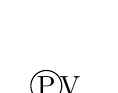
\begin{tikzpicture}[baseline=(p.base), plain/.style={}]
				\node (p) [plain] {P};
				\node (v) [plain, right=1.9ex of p.west] {V};
				\draw (p.center) ++(0,0.2pt) circle(1.3ex);
			\end{tikzpicture}
		}
		{v}{
			\hspace*{-1.4ex}	% this achieves better visually pleasing centering in the tables
			\small
			
\begin{tikzpicture}[baseline=(p.base), plain/.style={}]
				\node (p) [plain] {P};
				\node (v) [plain, right=1.95ex of p.west] {V};
				\draw (v.center) ++(0.2pt,0.5pt) circle(1.3ex);
			\end{tikzpicture}
		}
		{}{PV}
	}
}

% renders header cell for effects table
\NewDocumentCommand{\DetailEffectHead}{ m }{\cellcolor{PrintableLightGray}#1}

% effects table for instruction; optional parameter:
% - p = indicate Parity
% - v = indicate oVerflow
% - default = just PV
\NewDocumentEnvironment{DetailEffects}{ O{} O{Effects} +b }{   
	%                               /spacer
	%                               |/note
	\vspace{3pt}                   %||/SF     /ZF      /(YF)    /HF      /(XF)    /PV      /NF      /CF      |
	\begin{tabularx}{\linewidth}{@{}lXC{3.8ex}|C{3.8ex}|C{3.6ex}|C{3.8ex}|C{3.6ex}|C{3.8ex}|C{3.8ex}|C{3.8ex}|@{}}
		% we need to use hhline because \cellcolor renders on top of cline/hline, and we can't use \rowcolor because we only want some cells to use background...
		\hhline{~~|*{8}{-|}}

		\multicolumn{2}{@{}X}{\textbf{#2}} &
		\multicolumn{1}{|c|}{\DetailEffectHead{SF}} &
		\DetailEffectHead{ZF} &
		\DetailEffectHead{} &
		\DetailEffectHead{HF} &
		\DetailEffectHead{} &
		\DetailEffectHead{\DetailParityOverflow{#1}} &
		\DetailEffectHead{NF} &
		\DetailEffectHead{CF}\notet\noteb\\[1pt]\cline{3-10}

		#3

	\end{tabularx}
	\vspace{2pt}
}{}

% effects details
\NewDocumentEnvironment{DetailEffectsFlags}{ +b }{
	{
	\vspace{0pt}
	\renewcommand{\arraystretch}{0.5}	% setting default row spacing low will allow us to manipulate individual rows to be taller (see \DetailFlag)
	\begin{tabularx}{\linewidth}{@{}llR{3.35cm}X}

		#1

	\end{tabularx}
	\vspace{2pt}
	}
}{}

% common flag result descriptions
\NewDocumentCommand{\DetailFlagResultHalfBorrow}{ s }{borrow from bit 4\IfBooleanTF{#1}{ (bit 12 for 16-bit)}{}}
\NewDocumentCommand{\DetailFlagResultBorrow}{ s }{borrow from bit 8\IfBooleanTF{#1}{ (bit 16 for 16-bit)}{}}
\NewDocumentCommand{\DetailFlagResultHalfCarry}{ s }{carry from bit 3\IfBooleanTF{#1}{ (bit 11 for 16-bit)}{}}
\NewDocumentCommand{\DetailFlagResultCarry}{ s }{carry from bit 7\IfBooleanTF{#1}{ (bit 15 for 16-bit)}{}}
\newcommand{\DetailFlagResultOverflowListBottomSpacing}{\vspace*{-4ex}}
\newcommand{\DetailFlagResultSign}[1][]{\IfEq{#1}{}{result}{{\tt #1}} is negative (bit {\tt 7} is set)}
\newcommand{\DetailFlagResultZero}[1][]{\IfEq{#1}{}{result}{{\tt #1}} is {\tt 0}}
\newcommand{\DetailFlagResultParity}[1][]{\IfEq{#1}{}{result}{{\tt #1}} has even number of bits set}
\newcommand{\DetailFlagResultOverflow}{
	\DetailFlagsList{
		\item both operands positive and result negative
		\item both operands negative and result positve
	}
	\DetailFlagResultOverflowListBottomSpacing % we don't want additional space below the table, otherwise next item would have larger gap
}

% describes the given flag in details
% #1 mandatory flag name, empty will leave less space before this row
% #2 mandatory prefix before description
% #3 mandatory description
% #4 optional, if "p" some vertical "prefix" space is inserted above
% note use of \rule when #1 (flag name) is empty - we want to have less spacing before next row in such case to keep all rows of the same flag closer together (don't use both, #4=p and empty #1 since they both set rules, results may be unpredictable)
\NewDocumentCommand{\DetailFlag}{ m m m O{} }{
	& \textbf{#1} & #2 & #3 
	\IfEq{#4}{p}{
		\rule{0pt}{1ex}
		\rule[-2ex]{0pt}{0pt}
	}{}
	\IfEq{#1}{}{}{
		\rule[2.5ex]{0pt}{0pt}
	} \\[2pt]
}
% concrete flags (so we don't have to type in the names as strings)
% #1 optional prefix before description (default = "set if:")
% #2 optional name of the flag, empty will leave less space before this row
% #3 mandatory description
% #4 * to add some vertical spacing before the item, empty to leave default
\NewDocumentCommand{\DetailFlagSF}{ O{set if:} O{SF} m s }{\DetailFlag{#2}{#1}{#3}[\IfBooleanTF{#4}{p}{}]}
\NewDocumentCommand{\DetailFlagZF}{ O{set if:} O{ZF} m s }{\DetailFlag{#2}{#1}{#3}[\IfBooleanTF{#4}{p}{}]}
\NewDocumentCommand{\DetailFlagHF}{ O{set if:} O{HF} m s }{\DetailFlag{#2}{#1}{#3}[\IfBooleanTF{#4}{p}{}]}
\NewDocumentCommand{\DetailFlagPV}{ O{set if:} O{PV} m s }{\DetailFlag{#2}{#1}{#3}[\IfBooleanTF{#4}{p}{}]}
\NewDocumentCommand{\DetailFlagNF}{ O{set if:} O{NF} m s }{\DetailFlag{#2}{#1}{#3}[\IfBooleanTF{#4}{p}{}]}
\NewDocumentCommand{\DetailFlagCF}{ O{set if:} O{CF} m s }{\DetailFlag{#2}{#1}{#3}[\IfBooleanTF{#4}{p}{}]}

% creates a list with specific margins and spacing to be used within detail flags descriptions
\newcommand{\DetailFlagsList}[1]{
	\vspace{-3ex}
	\setlist{leftmargin=1em,after=\vspace{-2ex}}
	\begin{itemize}
		\setlength\itemsep{-1pt}
		#1
	\end{itemize}
}

% this is used where additional comments are needed below flags table (actually, technically, from LaTeX point of view, from within the table itself); each item should be provided with `\item` command
\newcommand{\DetailFlagsComments}[1]{ 
	& & \multicolumn{8}{p{7.8cm}}{
		\vspace{1ex}	% compensate for -3ex from \DetailFlagsList, we want -2ex
		\DetailFlagsList{#1}
		\vspace{2ex}	% compenase for -2ex from \DetailFlagsList, we want default
	} \\[-3ex]
}


% ▀▀█▀▀ ▀█▀ ▒█▀▄▀█ ▀█▀ ▒█▄░▒█ ▒█▀▀█   ▒█▀▀▀█ ▒█▀▀▀ ▒█▀▀█ ▀▀█▀▀ ▀█▀ ▒█▀▀▀█ ▒█▄░▒█ 
% ░▒█░░ ▒█░ ▒█▒█▒█ ▒█░ ▒█▒█▒█ ▒█░▄▄   ░▀▀▀▄▄ ▒█▀▀▀ ▒█░░░ ░▒█░░ ▒█░ ▒█░░▒█ ▒█▒█▒█ 
% ░▒█░░ ▄█▄ ▒█░░▒█ ▄█▄ ▒█░░▀█ ▒█▄▄█   ▒█▄▄▄█ ▒█▄▄▄ ▒█▄▄█ ░▒█░░ ▄█▄ ▒█▄▄▄█ ▒█░░▀█

% the main timing environment; optional parameter allows specifying the title, defaults to "Timing"
\NewDocumentEnvironment{DetailTiming}{ O{Timing} +b }{
	\vspace{1pt}
	\begin{tabularx}{0.8\textwidth}{@{}lXccrrrr@{}}
		\multicolumn{2}{@{}X}{\textbf{#1}} & Mc & Ts & 3.5MHz & 7MHz & 14MHz & 28MHz \\[1pt]
		#2
	\end{tabularx}
}{}

% formats individual timing item; parameters
% - optional: number of digits to round to (defaults to 2)
% - T states
% - CPU frequency to adjust to
% note: this is meant to be used internally by other detail time commands, the only reason for implementing it as its own command is to unify formatting
% note: command must be single line to avoid spaces being added on either side...
\newcommand{\DetailTimeItem}[3][2]{\nprounddigits{#1}{\small {\tt \numprint{\fpeval{#2/#3}}}$\mu$s}}

% individual time; parameters:
% - optional description, omit if none (which is the default)
% - number of machine cycles
% - number to T states
% note: the times in microsec are automatically calculated from Ts
\newcommand{\DetailTimeRegular}[3][]{
	& #1 & #2 & #3 & 
		\DetailTimeItem[1]{#3}{3.5} & 
		\DetailTimeItem{#3}{7} &
		\DetailTimeItem{#3}{14} &
		\DetailTimeItem{#3}{28} \\
}
% same as `DetailTimeRegular` but uses mono font for first (optional) parameter
\newcommand{\DetailTime}[3][]{\DetailTimeRegular[{\tt #1}]{#2}{#3}}


% ▒█▀▄▀█ ▀█▀ ▒█▀▀▀█ ▒█▀▀█ 
% ▒█▒█▒█ ▒█░ ░▀▀▀▄▄ ▒█░░░ 
% ▒█░░▒█ ▄█▄ ▒█▄▄▄█ ▒█▄▄█

% notes with additional information about instruction; optional parameter: if not empty, it is interpretted as size, empty will yield no space (this is used for multiple successive notes so that they are more compact vertically)
\newcommand{\DetailNote}[2][1.5ex]{
	\IfEq{#1}{}{
		% if empty, no spacing should be applied
	}{
		% otherwise interpret #1 as size and use for vertical spacing
		\vspace*{#1}
	}
	% either way, print note in smaller font
	{\small \normalfont{#2}}
}

% references to multiple items from other pages; parameters:
% #1 items description
% #2 page references (from `label` command)
\newcommand{\DetailItemsSeePageReference}[2]{
	\vspace*{-1.5em}
	\desclabelstyle{\pushlabel}
	\DetailMnemonic{#1}
	\desclabelstyle{\multilinelabel}
	\DetailNote{#2}
}
% reference to single item from another page
% #1 mnemonic (also serves to form the page reference itself)
\newcommand{\DetailItemSeePageReference}[1]{
	\DetailItemsSeePageReference{#1}{See page \DetailItemPageRef{#1}}
}


The following pages describe all instructions in detail. Alphabetical order is used as much as possible, but some deviations were made to better fit to pages. Each instruction includes:

\begin{itemize}
	\setlength\itemsep{1pt}
	\item Mnemonic
	\item Symbolic operation for quick info on what instruction does
	\item All variants (where applicable)
	\item Description with further details
	\item Effects on flags
	\item Timing table with machine cycles, T states and time required for execution on different CPU speeds
\end{itemize}

Where possible, multiple variants of same instruction are grouped together and where multiple timings are possible, timing table is sorted from quickest to slowest.

\pagebreak
\thispagestyle{plain} % use toc style without headers for this explanation page, it better matches chapter start page


\subsubsection{Flags}

\newcommand{\DetailsFlagTableList}[1]{
	\vspace*{-2ex}
	\setlist{leftmargin=1em,after=\vspace{-2ex}}
	\begin{itemize}
		\setlength\itemsep{-4pt}
		#1
	\end{itemize}
}

\newcommand{\DetailsFlagTableParagraph}{\vspace{1ex}}

{	
	\renewcommand{\arraystretch}{1.5}

	\begin{tabularx}{\linewidth}{cX}
		\FlagSF{} &
			\textbf{Sign Flag} is set to twos-complement of the most-significant bit (bit 7) of the result of an instruction. If the result is positive (bit 7 is {\tt 0}), \FlagSF{} is set, and if the result is negative (bit 7 is {\tt 1}), \FlagSF{} is reset. This leaves bits 0-6 to represent the value. Positive numbers range from {\tt 0} to {\tt 127} and negative from {\tt -1} to {\tt -128}.
			\\

		\FlagZF{} &
			\textbf{Zero Flag} depends on whether the result of an instruction is {\tt 0}. \FlagZF{} is set if the result if {\tt 0} and reset otherwise.
			\\

		\FlagHF{} &
			\textbf{Half Carry Flag} represents a carry or borrow status between bits 3 and 4 of an 8-bit arithmetic operation (bits 11 and 12 for 16-bit operations). Set if:
		
			\DetailsFlagTableList{
				\item A carry from bit 3 to bit 4 occurs during addition (bit 11 to 12 for 16-bit operations)
				\item A borrow from bit 4 occurs during subtraction (from bit 12 for 16-bit operations)
			}
			\\

		\FlagPV{} &
			\textbf{Parity/Overflow Flag} value depends on the type of the operation.
			
			\DetailsFlagTableParagraph
			For arithmetic operations, \FlagPV{} indicates an overflow. The flag is set when the sign of the result is different from the sign of the operands:
			
			\DetailsFlagTableList{
				\item all operands are positive but the result is negative or
				\item all operands are negative but the result is positive
			}
			
			\DetailsFlagTableParagraph
			For logical and rotate operations, \FlagPV{} indicates the parity of the result. The number of set bits in the result are counted. If the total is an even value, \FlagPV{} is set. If the total is odd, \FlagPV{} is reset.
			\\

		\FlagNF{} &
			\textbf{Add/Subtract Flag} is used primarily for {\tt DAA} instruction to distinguish between add and subtract operations. But other instructions may also affect it as described in the following pages.
			\\

		\textbf{CF} &
			\textbf{Carry Flag} represents a carry or borrow status for arithmetic operations. \textbf{CF} is set if add instruction generates a carry, or subtract generates a borrow.
			
			\DetailsFlagTableParagraph
			For rotate and shift instructions, \textbf{CF} is used:
			
			\DetailsFlagTableList{
				\item as a link between least-significat and most significant bit for {\tt RLA}, {\tt RL}, {\tt RRA} and {\tt RR}
				\item contains the value shifted out of bit 7 for {\tt RLC}, {\tt RLCA} and {\tt SLA}
				\item contains the value shifted out of bit 0 for {\tt RRC}, {\tt RRCA}, {\tt SRA} and {\tt SRL}
			}

			\DetailsFlagTableParagraph
			Finally, some instructions directly affect the value of \textbf{CF}:

			\DetailsFlagTableList{
				\item reset with {\tt AND}, {\tt OR} and {\tt XOR}
				\item set with {\tt SCF}
				\item completed with {\tt CCF}
			}
			\\
	\end{tabularx}
}


\subsubsection{Effects}

\begin{tabular}{cl}
	{\tt 0} & Flag is set to {\tt 0} \\
	{\tt 1} & Flag is set to {\tt 1} \\
	{\tt \FS} & Flag is modified according to operation \\
	{\tt \FN} & Flag is not affected \\
	{\tt \FU} & Effect on flag is unpredictable \\
	{\tt \FX} & Special case, see notes below effects table \\
	\DetailParityOverflow{v} & P/V flag is used as overflow \\
	\DetailParityOverflow{p} & P/V flag is used as parity \\
	\DetailParityOverflow{} & P/V is undefined or indicates other result \\
\end{tabular}


\subsubsection{Abbreviations}

\begin{tabularx}{\textwidth}{lX}
	{\tt r} & 
		8-bit register {\tt A}-{\tt L} \\
	{\tt n} &
		8-bit immediate value \\
	{\tt rr} & 
		16-bit register pair {\tt AF}, {\tt BC}, {\tt DE}, {\tt HL}, {\tt IX}, {\tt IY}, {\tt SP} (note in some cases particular register pairs may use different timing from the rest; if so, those will be explicitly indicated in their own line; {\tt rr} may still be used, though in those cases it will cover the remaining registers only) \\
	{\tt nn} & 
		16-bit immediate value \\
	{\tt s} &
		Placeholder for argument when multiple variants are possible \\
	{\tt d} &
		If instruction takes 2 operands, {\tt d} indicates destination and {\tt s} source \\
	\UNDOC & Indicates undocumented instruction \\
	\ZXN & Indicates ZX Spectrum Next extended instruction \\		
\end{tabularx}


\pagebreak
\IntentionallyEmpty
\pagebreak



\begin{basedescript}{
	% setup basedescript styling for labels
	\desclabelstyle{\multilinelabel}
	\desclabelwidth{3cm}}

	% setup spacing between items
	\setlength\itemsep{1.5em}

	\pagebreak


	%----------------------------------------------------------------------------------------------------------------------
	% ███████████████████████████████████████████████████████████████████
	% █▄─▄█▄─▀█▄─▄█─▄▄▄▄█─▄─▄─█▄─▄▄▀█▄─██─▄█─▄▄▄─█─▄─▄─█▄─▄█─▄▄─█▄─▀█▄─▄█
	% ██─███─█▄▀─██▄▄▄▄─███─████─▄─▄██─██─██─███▀███─████─██─██─██─█▄▀─██
	% ▀▄▄▄▀▄▄▄▀▀▄▄▀▄▄▄▄▄▀▀▄▄▄▀▀▄▄▀▄▄▀▀▄▄▄▄▀▀▄▄▄▄▄▀▀▄▄▄▀▀▄▄▄▀▄▄▄▄▀▄▄▄▀▀▄▄▀
	%----------------------------------------------------------------------------------------------------------------------

	\begin{DetailItem}{ADC}{d,s}
		{\IH{AD}d with \IH{C}arry}
		{\SymADC{d}{s}}

		\begin{DetailVariants}[p{1.9cm}p{1.9cm}Xp{2.8cm}p{2.4cm}]
			\textnormal{8 bit} & \textnormal{8 bit} & \textnormal{8 bit} & \textnormal{8 bit} & \textnormal{16 bit} \\
			ADC A,A	& ADC A,E	& ADC A,(HL)	& ADC A,IXH\UNDOC	& ADC HL,BC \\
			ADC A,B	& ADC A,H	& ADC A,(IX+d)	& ADC A,IXL\UNDOC	& ADC HL,DE \\
			ADC A,C	& ADC A,L	& ADC A,(IY+d)	& ADC A,IYH\UNDOC	& ADC HL,HL \\
			ADC A,D	& ADC A,n	& 				& ADC A,IYL\UNDOC	& ADC HL,SP \\
		\end{DetailVariants}
		
		Adds source operand {\tt s} or contents of the memory location addressed by {\tt s} and value of carry flag to destination {\tt d}. Result is then stored to destination {\tt d}.

		\begin{DetailEffects}[v]
			\FlagsADCr[8-bit]
			\FlagsADCrr[16-bit]
		\end{DetailEffects}

		\begin{DetailEffectsFlags}
			\DetailFlagSF{\DetailFlagResultSign}
			\DetailFlagZF{\DetailFlagResultZero}
			\DetailFlagHF{\DetailFlagResultHalfCarry}*
			\DetailFlagPV{\DetailFlagResultOverflow}*
			\DetailFlagCF{\DetailFlagResultCarry}
		\end{DetailEffectsFlags}

		\begin{DetailTiming}
			\DetailTime[A,r]{1}{4}
			\DetailTime[A,n]{2}{7}
			\DetailTime[A,(HL)]{2}{7}
			\DetailTime[HL,rr]{4}{15}
			\DetailTime[A,(IX+d)]{5}{19}
			\DetailTime[A,(IY+d)]{5}{19}
		\end{DetailTiming}
		
	\end{DetailItem}
	
	\pagebreak

	%----------------------------------------------------------------------------------------------------------------------
	% ███████████████████████████████████████████████████████████████████
	% █▄─▄█▄─▀█▄─▄█─▄▄▄▄█─▄─▄─█▄─▄▄▀█▄─██─▄█─▄▄▄─█─▄─▄─█▄─▄█─▄▄─█▄─▀█▄─▄█
	% ██─███─█▄▀─██▄▄▄▄─███─████─▄─▄██─██─██─███▀███─████─██─██─██─█▄▀─██
	% ▀▄▄▄▀▄▄▄▀▀▄▄▀▄▄▄▄▄▀▀▄▄▄▀▀▄▄▀▄▄▀▀▄▄▄▄▀▀▄▄▄▄▄▀▀▄▄▄▀▀▄▄▄▀▄▄▄▄▀▄▄▄▀▀▄▄▀
	%----------------------------------------------------------------------------------------------------------------------

	\begin{DetailItem}{ADD}{d,s}
		{\IH{ADD}}
		{\SymADD{d}{s}}

		\begin{DetailVariants}[p{1.9cm}Xp{2.3cm}p{2.3cm}p{2.4cm}]
			\textnormal{8-bit} & \textnormal{8-bit} & \textnormal{16-bit} & \textnormal{16-bit} & \textnormal{ZX Next} \\
			ADD A,A & ADD A,(HL) 		& ADD IX,BC & ADD HL,BC	& ADD BC,A\ZXN \\
			ADD A,B & ADD A,(IX+d)		& ADD IX,DE & ADD HL,DE & ADD DE,A\ZXN \\
			ADD A,C & ADD A,(IY+d)		& ADD IX,IX & ADD HL,HL & ADD HL,A\ZXN \\
			ADD A,D & ADD A,IXH\UNDOC	& ADD IX,SP & ADD HL,SP & ADD BE,nn\ZXN \\ 
			ADD A,E & ADD A,IXL\UNDOC	& ADD IY,BC & 			& ADD DE,nn\ZXN \\
			ADD A,H & ADD A,IYH\UNDOC	& ADD IY,DE & 			& ADD HL,nn\ZXN \\
			ADD A,L & ADD A,IYL\UNDOC	& ADD IY,IY \\
			ADD A,n & 					& ADD IY,SP \\
		\end{DetailVariants}
		
		Similar to {\tt ADC} except carry flag is not used in calculation: adds operand {\tt s} or contents of the memory location addressed by {\tt s} to destination {\tt d}. Result is then stored to destination {\tt d}.

		ZX Next Extended instructions for adding {\tt A} to 16-bit register pair, zero extend {\tt A} to 16-bits.

		\begin{DetailEffects}[v]
			\FlagsADDr[8-bit]
			\FlagsADDrr[16-bit]
		\end{DetailEffects}

		\begin{DetailEffectsFlags}
			\DetailFlagSF[8-bit only, set if:]{\DetailFlagResultSign}
			\DetailFlagZF[8-bit only, set if:]{\DetailFlagResultZero}
			\DetailFlagHF{\DetailFlagResultHalfCarry*}*
			\DetailFlagPV[8-bit only, set if:]{\DetailFlagResultOverflow}*
			\DetailFlagCF{\DetailFlagResultCarry*}
		\end{DetailEffectsFlags}

		\begin{DetailEffects}
			\FlagsADDrra[\tt ADD rr,A\ZXN]
			\FlagsADDrrnn[\tt ADD rr,nn\ZXN]
		\end{DetailEffects}

		\begin{DetailTiming}
			\DetailTime[A,r]{1}{4}
			\DetailTime[A,n]{2}{7}
			\DetailTime[A,(HL)]{2}{7}
			\DetailTime[rr,A\ZXN]{2}{8}
			\DetailTime[HL,rr]{3}{11}
			\DetailTime[IX,rr]{4}{15}
			\DetailTime[IY,rr]{4}{15}
			\DetailTime[rr,nn\ZXN]{4}{16}
			\DetailTime[A,(IX+d)]{5}{19}
			\DetailTime[A,(IY+d)]{5}{19}
		\end{DetailTiming}

	\end{DetailItem}

	\pagebreak

	%----------------------------------------------------------------------------------------------------------------------
	% ███████████████████████████████████████████████████████████████████
	% █▄─▄█▄─▀█▄─▄█─▄▄▄▄█─▄─▄─█▄─▄▄▀█▄─██─▄█─▄▄▄─█─▄─▄─█▄─▄█─▄▄─█▄─▀█▄─▄█
	% ██─███─█▄▀─██▄▄▄▄─███─████─▄─▄██─██─██─███▀███─████─██─██─██─█▄▀─██
	% ▀▄▄▄▀▄▄▄▀▀▄▄▀▄▄▄▄▄▀▀▄▄▄▀▀▄▄▀▄▄▀▀▄▄▄▄▀▀▄▄▄▄▄▀▀▄▄▄▀▀▄▄▄▀▄▄▄▄▀▄▄▄▀▀▄▄▀
	%----------------------------------------------------------------------------------------------------------------------

	\begin{DetailItem}{AND}{s}
		{bitwise \IH{AND}}
		{\SymAND{s}}

		\begin{DetailVariants}[4]
			AND A\\
			AND B\\
			AND C\\
			AND D

			\columnbreak
			AND E\\
			AND H\\
			AND L\\
			AND n
			
			\columnbreak
			AND (HL)\\
			AND (IX+d)\\
			AND (IY+d)

			\columnbreak
			AND IXH\UNDOC\\
			AND IXL\UNDOC\\
			AND IYH\UNDOC\\
			AND IYL\UNDOC
		\end{DetailVariants}

		\begin{tabularx}{\linewidth}{@{}Xl}
			Performs bitwise AND between accumulator {\tt A} and the given operand. The result is then stored back to the accumulator. Individual bits are AND'ed as shown on the right:

			&

			\begin{tabular}[t]{cc|c}
				{\tt A} & {\tt s} & Result \\
				\hline
				{\tt 0} & {\tt 0} & {\tt 0} \\
				{\tt 0} & {\tt 1} & {\tt 0} \\
				{\tt 1} & {\tt 0} & {\tt 0} \\
				{\tt 1} & {\tt 1} & {\tt 1} \\
			\end{tabular}

			\\
		\end{tabularx}

		\begin{DetailEffects}[p]
			\FlagsANDr
		\end{DetailEffects}

		\begin{DetailEffectsFlags}
			\DetailFlagSF{\DetailFlagResultSign}
			\DetailFlagZF{\DetailFlagResultZero}
			\DetailFlagPV{\DetailFlagResultParity}
		\end{DetailEffectsFlags}

		\begin{DetailTiming}
			\DetailTime[r]{1}{4}
			\DetailTime[n]{2}{7}
			\DetailTime[(HL)]{2}{7}
			\DetailTime[(IX+d)]{5}{19}
			\DetailTime[(IY+d)]{5}{19}
		\end{DetailTiming}

	\end{DetailItem}

	%----------------------------------------------------------------------------------------------------------------------
	% ███████████████████████████████████████████████████████████████████
	% █▄─▄█▄─▀█▄─▄█─▄▄▄▄█─▄─▄─█▄─▄▄▀█▄─██─▄█─▄▄▄─█─▄─▄─█▄─▄█─▄▄─█▄─▀█▄─▄█
	% ██─███─█▄▀─██▄▄▄▄─███─████─▄─▄██─██─██─███▀███─████─██─██─██─█▄▀─██
	% ▀▄▄▄▀▄▄▄▀▀▄▄▀▄▄▄▄▄▀▀▄▄▄▀▀▄▄▀▄▄▀▀▄▄▄▄▀▀▄▄▄▄▄▀▀▄▄▄▀▀▄▄▄▀▄▄▄▄▀▄▄▄▀▀▄▄▀
	%----------------------------------------------------------------------------------------------------------------------

	\begin{DetailItem}{BIT}{b,s}
		{test \IH{BIT}}
		{\SymBIT{s}}

		\begin{DetailVariants}
			BIT b,A\\
			BIT b,B\\
			BIT b,C\\
			BIT b,D

			\columnbreak
			BIT b,E\\
			BIT b,H\\
			BIT b,L
			
			\columnbreak
			BIT b,(HL)\\
			BIT b,(IX+d)\\
			BIT b,(IY+d)
		\end{DetailVariants}

		Tests specified bit {\tt b} ({\tt 0-7}) of the given register {\tt s} or contents of memory addressed by {\tt s} and sets zero flag according to result; if bit was 1, \FlagZF{} is 0 and vice versa.

		\begin{DetailEffects}
			\FlagsBITr
		\end{DetailEffects}

		\begin{DetailEffectsFlags}
			\DetailFlagZF{bit {\tt b} of the given source argument is {\tt 0}}
		\end{DetailEffectsFlags}

		\begin{DetailTiming}
			\DetailTime[b,r]{2}{8}
			\DetailTime[b,(HL)]{3}{12}
			\DetailTime[b,(IX+d)]{5}{20}
			\DetailTime[b,(IY+d)]{5}{20}
		\end{DetailTiming}

	\end{DetailItem}

	% these instructions should be here in alphabetical order, but I want them to be placed on the same page spread so reader can check the differences easily
	\DetailItemsSeePageReference{BRLC, BSLA, BSRA, BSRF, BSRL}{See pages \DetailItemPageRef{BRLC} and \DetailItemPageRef{BSRL}}

	%----------------------------------------------------------------------------------------------------------------------
	% ███████████████████████████████████████████████████████████████████
	% █▄─▄█▄─▀█▄─▄█─▄▄▄▄█─▄─▄─█▄─▄▄▀█▄─██─▄█─▄▄▄─█─▄─▄─█▄─▄█─▄▄─█▄─▀█▄─▄█
	% ██─███─█▄▀─██▄▄▄▄─███─████─▄─▄██─██─██─███▀███─████─██─██─██─█▄▀─██
	% ▀▄▄▄▀▄▄▄▀▀▄▄▀▄▄▄▄▄▀▀▄▄▄▀▀▄▄▀▄▄▀▀▄▄▄▄▀▀▄▄▄▄▄▀▀▄▄▄▀▀▄▄▄▀▄▄▄▄▀▄▄▄▀▀▄▄▀
	%----------------------------------------------------------------------------------------------------------------------

	\begin{DetailItem}{CALL}{nn}
		{\IH{CALL} subroutine}
		{\SymCALL{nn}}

		Pushes program counter {\tt PC} to stack and calls subroutine at the given location {\tt nn} by changing {\tt PC} to point to address {\tt nn}.

		\begin{DetailEffects}
			\FlagsCALLnn
		\end{DetailEffects}
		
		\begin{DetailTiming}
			\DetailTime{5}{17}
		\end{DetailTiming}

	\end{DetailItem}

	%----------------------------------------------------------------------------------------------------------------------
	% ███████████████████████████████████████████████████████████████████
	% █▄─▄█▄─▀█▄─▄█─▄▄▄▄█─▄─▄─█▄─▄▄▀█▄─██─▄█─▄▄▄─█─▄─▄─█▄─▄█─▄▄─█▄─▀█▄─▄█
	% ██─███─█▄▀─██▄▄▄▄─███─████─▄─▄██─██─██─███▀███─████─██─██─██─█▄▀─██
	% ▀▄▄▄▀▄▄▄▀▀▄▄▀▄▄▄▄▄▀▀▄▄▄▀▀▄▄▀▄▄▀▀▄▄▄▄▀▀▄▄▄▄▄▀▀▄▄▄▀▀▄▄▄▀▄▄▄▄▀▄▄▄▀▀▄▄▀
	%----------------------------------------------------------------------------------------------------------------------

	\begin{DetailItem}{CALL c,nn}{}
		{\IH{CALL} subroutine conditionally}
		{\SymCALLc{nn}}

		\vspace{1ex} % we need some vertical space to achieve same separation as multicols
		\begin{tabular}{@{}llcll}			
			{\tt CALL C,nn} & calls if \FlagCF{} is set & &
				{\tt CALL M,nn} & calls if \FlagSF{} is set\\
			{\tt CALL NC,nn} & calls if \FlagCF{} is reset & &
				{\tt CALL P,nn} & calls if \FlagSF{} is reset\\
			{\tt CALL Z,nn} & calls if \FlagZF{} is set & &
				{\tt CALL PE,nn} & calls if \FlagPV{} is set\\
			{\tt CALL NZ,nn} & calls if \FlagZF{} is reset & &
				{\tt CALL PO,nn} & calls if \FlagPV{} is reset\\
		\end{tabular}

		If the given condition is met, {\tt CALL nn} is performed, as described above.

		\begin{DetailEffects}
			\FlagsCALLccnn
		\end{DetailEffects}

		\begin{DetailTiming}
			\DetailTime[c\normalfont{=false}]{3}{10}
			\DetailTime[c\normalfont{=true}]{5}{17}
		\end{DetailTiming}

	\end{DetailItem}

	\pagebreak

	%----------------------------------------------------------------------------------------------------------------------
	% ███████████████████████████████████████████████████████████████████
	% █▄─▄█▄─▀█▄─▄█─▄▄▄▄█─▄─▄─█▄─▄▄▀█▄─██─▄█─▄▄▄─█─▄─▄─█▄─▄█─▄▄─█▄─▀█▄─▄█
	% ██─███─█▄▀─██▄▄▄▄─███─████─▄─▄██─██─██─███▀███─████─██─██─██─█▄▀─██
	% ▀▄▄▄▀▄▄▄▀▀▄▄▀▄▄▄▄▄▀▀▄▄▄▀▀▄▄▀▄▄▀▀▄▄▄▄▀▀▄▄▄▄▄▀▀▄▄▄▀▀▄▄▄▀▄▄▄▄▀▄▄▄▀▀▄▄▀
	%----------------------------------------------------------------------------------------------------------------------

	\begin{DetailItem}{BRLC}{DE,B\ZXN}
		{\IH{B}arrel \IH{R}otate \IH{L}eft \IH{C}ircular}
		{\SymBRLC}

		Rotates value in register pair {\tt DE} left for the amount given in bits 3-0 (low nibble) of register {\tt B}. To rotate right, use formula: {\tt B=16-places}. The result is stored in {\tt DE}.

		\begin{DetailEffects}
			\FlagsBRLC
		\end{DetailEffects}

		\begin{DetailTiming}
			\DetailTime{2}{8}
		\end{DetailTiming}

	\end{DetailItem}

	%----------------------------------------------------------------------------------------------------------------------
	% ███████████████████████████████████████████████████████████████████
	% █▄─▄█▄─▀█▄─▄█─▄▄▄▄█─▄─▄─█▄─▄▄▀█▄─██─▄█─▄▄▄─█─▄─▄─█▄─▄█─▄▄─█▄─▀█▄─▄█
	% ██─███─█▄▀─██▄▄▄▄─███─████─▄─▄██─██─██─███▀███─████─██─██─██─█▄▀─██
	% ▀▄▄▄▀▄▄▄▀▀▄▄▀▄▄▄▄▄▀▀▄▄▄▀▀▄▄▀▄▄▀▀▄▄▄▄▀▀▄▄▄▄▄▀▀▄▄▄▀▀▄▄▄▀▄▄▄▄▀▄▄▄▀▀▄▄▀
	%----------------------------------------------------------------------------------------------------------------------

	\begin{DetailItem}{BSLA}{DE,B\ZXN}
		{\IH{B}arrel \IH{S}hift \IH{L}eft \IH{A}rithmetic}
		{\SymBSLA}

		Performs shift left of the value in register pair {\tt DE} for the amount given in lower 5 bits of register {\tt B}. The result is stored in {\tt DE}.

		\begin{DetailEffects}
			\FlagsBSLA
		\end{DetailEffects}
		
		\begin{DetailTiming}
			\DetailTime{2}{8}
		\end{DetailTiming}

	\end{DetailItem}

	%----------------------------------------------------------------------------------------------------------------------
	% ███████████████████████████████████████████████████████████████████
	% █▄─▄█▄─▀█▄─▄█─▄▄▄▄█─▄─▄─█▄─▄▄▀█▄─██─▄█─▄▄▄─█─▄─▄─█▄─▄█─▄▄─█▄─▀█▄─▄█
	% ██─███─█▄▀─██▄▄▄▄─███─████─▄─▄██─██─██─███▀███─████─██─██─██─█▄▀─██
	% ▀▄▄▄▀▄▄▄▀▀▄▄▀▄▄▄▄▄▀▀▄▄▄▀▀▄▄▀▄▄▀▀▄▄▄▄▀▀▄▄▄▄▄▀▀▄▄▄▀▀▄▄▄▀▄▄▄▄▀▄▄▄▀▀▄▄▀
	%----------------------------------------------------------------------------------------------------------------------

	\begin{DetailItem}{BSRA}{DE,B\ZXN}
		{\IH{B}arrel \IH{S}hift \IH{R}ight \IH{A}rithmetic}
		{\SymBSRA}

		Performs arithmetical shift right of the value in register pair {\tt DE} for the amount given in lower 5 bits of register {\tt B}. The result is stored in {\tt DE}.

		\begin{DetailEffects}
			\FlagsBSRA
		\end{DetailEffects}
		
		\begin{DetailTiming}
			\DetailTime{2}{8}
		\end{DetailTiming}

	\end{DetailItem}

	\pagebreak

	%----------------------------------------------------------------------------------------------------------------------
	% ███████████████████████████████████████████████████████████████████
	% █▄─▄█▄─▀█▄─▄█─▄▄▄▄█─▄─▄─█▄─▄▄▀█▄─██─▄█─▄▄▄─█─▄─▄─█▄─▄█─▄▄─█▄─▀█▄─▄█
	% ██─███─█▄▀─██▄▄▄▄─███─████─▄─▄██─██─██─███▀███─████─██─██─██─█▄▀─██
	% ▀▄▄▄▀▄▄▄▀▀▄▄▀▄▄▄▄▄▀▀▄▄▄▀▀▄▄▀▄▄▀▀▄▄▄▄▀▀▄▄▄▄▄▀▀▄▄▄▀▀▄▄▄▀▄▄▄▄▀▄▄▄▀▀▄▄▀
	%----------------------------------------------------------------------------------------------------------------------

	\begin{DetailItem}{BSRF}{DE,B\ZXN}
		{\IH{B}arrel \IH{S}hift \IH{R}ight \IH{F}ill-one}
		{\SymBSRF}

		Performs fill-one-way shift right of the value in register pair {\tt DE} for the amount given in lower 5 bits of register {\tt B}. The result is stored in {\tt DE}.

		\begin{DetailEffects}
			\FlagsBSRF
		\end{DetailEffects}
		
		\begin{DetailTiming}
			\DetailTime{2}{8}
		\end{DetailTiming}

	\end{DetailItem}

	%----------------------------------------------------------------------------------------------------------------------
	% ███████████████████████████████████████████████████████████████████
	% █▄─▄█▄─▀█▄─▄█─▄▄▄▄█─▄─▄─█▄─▄▄▀█▄─██─▄█─▄▄▄─█─▄─▄─█▄─▄█─▄▄─█▄─▀█▄─▄█
	% ██─███─█▄▀─██▄▄▄▄─███─████─▄─▄██─██─██─███▀███─████─██─██─██─█▄▀─██
	% ▀▄▄▄▀▄▄▄▀▀▄▄▀▄▄▄▄▄▀▀▄▄▄▀▀▄▄▀▄▄▀▀▄▄▄▄▀▀▄▄▄▄▄▀▀▄▄▄▀▀▄▄▄▀▄▄▄▄▀▄▄▄▀▀▄▄▀
	%----------------------------------------------------------------------------------------------------------------------

	\begin{DetailItem}{BSRL}{DE,B\ZXN}
		{\IH{B}arrel \IH{S}hift \IH{R}ight \IH{L}ogical}
		{\SymBSRL}

		Performs logical shift right of the value in register pair {\tt DE} for the amount given in lower 5 bits of register {\tt B}. The result is stored in {\tt DE}.

		\begin{DetailEffects}
			\FlagsBSRL
		\end{DetailEffects}
		
		\begin{DetailTiming}
			\DetailTime{2}{8}
		\end{DetailTiming}

	\end{DetailItem}

	% CALL instructions should be here in alphabetical order, but I placed them before B*** above so they can be in the same page spread
	\DetailItemSeePageReference{CALL}

	%----------------------------------------------------------------------------------------------------------------------
	% ███████████████████████████████████████████████████████████████████
	% █▄─▄█▄─▀█▄─▄█─▄▄▄▄█─▄─▄─█▄─▄▄▀█▄─██─▄█─▄▄▄─█─▄─▄─█▄─▄█─▄▄─█▄─▀█▄─▄█
	% ██─███─█▄▀─██▄▄▄▄─███─████─▄─▄██─██─██─███▀███─████─██─██─██─█▄▀─██
	% ▀▄▄▄▀▄▄▄▀▀▄▄▀▄▄▄▄▄▀▀▄▄▄▀▀▄▄▀▄▄▀▀▄▄▄▄▀▀▄▄▄▄▄▀▀▄▄▄▀▀▄▄▄▀▄▄▄▄▀▄▄▄▀▀▄▄▀
	%----------------------------------------------------------------------------------------------------------------------

	\begin{DetailItem}{CCF}{}
		{\IH{C}omplement \IH{C}arry \IH{F}lag}
		{\SymCCF}

		Complements (inverts) carry flag \FlagCF{}; if \FlagCF{} was {\tt 0} it's now {\tt 1} and vice versa. Previous value of \FlagCF{} is copied to \FlagHF{}.

		\begin{DetailEffects}
			\FlagsCCF
		\end{DetailEffects}

		
		\begin{DetailEffectsFlags}
			\DetailFlagHF[]{Documentation says original value of \FlagCF{} is copied to \FlagHF{}, however under my tests \FlagHF{} remained unchanged}
			\DetailFlagCF[]{if \FlagCF{} was {\tt 0} it's now {\tt 1} and vice versa}
		\end{DetailEffectsFlags}
		
		\begin{DetailTiming}
			\DetailTime{1}{4}
		\end{DetailTiming}

	\end{DetailItem}

	\pagebreak

	%----------------------------------------------------------------------------------------------------------------------
	% ███████████████████████████████████████████████████████████████████
	% █▄─▄█▄─▀█▄─▄█─▄▄▄▄█─▄─▄─█▄─▄▄▀█▄─██─▄█─▄▄▄─█─▄─▄─█▄─▄█─▄▄─█▄─▀█▄─▄█
	% ██─███─█▄▀─██▄▄▄▄─███─████─▄─▄██─██─██─███▀███─████─██─██─██─█▄▀─██
	% ▀▄▄▄▀▄▄▄▀▀▄▄▀▄▄▄▄▄▀▀▄▄▄▀▀▄▄▀▄▄▀▀▄▄▄▄▀▀▄▄▄▄▄▀▀▄▄▄▀▀▄▄▄▀▄▄▄▄▀▄▄▄▀▀▄▄▀
	%----------------------------------------------------------------------------------------------------------------------

	\begin{DetailItem}{CP}{s}
		{\IH{C}om\IH{P}are}
		{\SymCP{s}}

		\begin{DetailVariants}[4]
			CP A\\
			CP B\\
			CP C\\
			CP D

			\columnbreak
			CP E\\
			CP H\\
			CP L\\
			CP n

			\columnbreak
			CP (HL)\\
			CP (IX+d)\\
			CP (IY+d)

			\columnbreak
			CP IXH\UNDOC\\
			CP IXL\UNDOC\\
			CP IYH\UNDOC\\
			CP IYL\UNDOC
		\end{DetailVariants}

		Operand {\tt s} or content of the memory location addressed by {\tt s} is subtracted from accumulator {\tt A}. Status flags are updated according to the result, but the result is then discarded (value of {\tt A} is not changed).

		\begin{DetailEffects}[v]
			\FlagsCPr
		\end{DetailEffects}

		\begin{DetailEffectsFlags}
			\DetailFlagHF{\DetailFlagResultHalfBorrow}*
			\DetailFlagPV{
				\DetailFlagsList{
					\item {\tt A} and {\tt s} positive and {\tt A-s} result negative
					\item {\tt A} and {\tt s} negative and {\tt A-s} result positve
				}
				\DetailFlagResultOverflowListBottomSpacing % we don't want additional space below the table, otherwise next item would have larger gap
			}
		\end{DetailEffectsFlags}

		Other flags are set like this when {\tt A} is greater than, equal or less than {\tt s}:

		\begin{DetailEffects}[v][]
			\Flags[A$>$s]{0}{0}{\FS}{\FS}{1}{0}
			\Flags[A$=$s]{0}{1}{\FS}{\FS}{1}{0}
			\Flags[A$<$s]{1}{0}{\FS}{\FS}{1}{1}
		\end{DetailEffects}

		With this in mind, we can derive the programs for common comparisons:

		\newcommand{\CPExampleTitle}[1]{{\tt #1}\vspace{-1.5ex}}

		%-----------------------------------------------------------------------------------------------------
		\begin{multicols}{2}
			\CPExampleTitle{A=s}
			\begin{tcblisting}{right skip=1em}
	CP s
	JP Z, true ; A=s?
false: ; A!=s
true:   ; A=s
			\end{tcblisting}

			\CPExampleTitle{A$\neq$s}
			\begin{tcblisting}{}
	CP s
	JP NZ, true ; A!=s?
false: ; A=s
true:   ; A!=s
			\end{tcblisting}
		\end{multicols}

		%-----------------------------------------------------------------------------------------------------
		\begin{multicols}{2}
			\CPExampleTitle{A$\leqslant$s}
			\begin{tcblisting}{right skip=1em}
	CP s
	JP M, true  ; A<s?
	JP Z, true  ; A=s?
false: ; A>s
true:   ; A<=s
			\end{tcblisting}

			\columnbreak
			\CPExampleTitle{A<s}
			\begin{tcblisting}{}
	CP s
	JP M, true ; A<s?
false: ; A>=s
true:   ; A<s
			\end{tcblisting}
		\end{multicols}

		%-----------------------------------------------------------------------------------------------------
		\begin{multicols}{2}
			\CPExampleTitle{A$\geqslant$s}
			\begin{tcblisting}{right skip=1em}
	CP s
	JP M, false ; A<s?
true:   ; A>=s
false: ; A<s
			\end{tcblisting}

			\columnbreak
			\CPExampleTitle{A>s}
			\begin{tcblisting}{}
	CP s
	JP M, false ; A<s?
	JP Z, false ; A=s?
true:   ; A>s
false: ; A<=s
			\end{tcblisting}
		\end{multicols}

		\DetailNote[-1ex]{
			Note: the examples use two labels to emphasize both results. But only one is needed. Furthermore, depending on the actual needs, the programs can also use no label at all. For example, we can use {\tt RET} instead of {\tt JP} when used within a subroutine, and the desired outcome is to return if the condition is not met:
		}

		%-----------------------------------------------------------------------------------------------------
		\begin{multicols}{2}
			\CPExampleTitle{A=s}
			\begin{tcblisting}{right skip=1em}
	CP s
	RET NZ ; A!=s?
	; A=s
			\end{tcblisting}

			\CPExampleTitle{A$\neq$s}
			\begin{tcblisting}{}
	CP s
	RET Z ; A=s?
	; A!=s
			\end{tcblisting}
		\end{multicols}

		%-----------------------------------------------------------------------------------------------------
		\begin{multicols}{2}
			\CPExampleTitle{A$\leqslant$s}
			\begin{tcblisting}{right skip=1em}
	CP s
	JP M, true  ; A<s?
	JP Z, true  ; A=s?
	RET         ; A>s
true:   ; A<=s
			\end{tcblisting}

			\columnbreak
			\CPExampleTitle{A<s}
			\begin{tcblisting}{}
	CP s
	RET P ; A>=s?
	; A<s
			\end{tcblisting}
		\end{multicols}

		%-----------------------------------------------------------------------------------------------------
		\begin{multicols}{2}
			\CPExampleTitle{A$\geqslant$s}
			\begin{tcblisting}{right skip=1em}
	CP s
	RET M ; A<s?
	; A>=s
			\end{tcblisting}

			\CPExampleTitle{A>s}
			\begin{tcblisting}{}
	CP s
	RET M ; A<s?
	RET Z ; A=s?
	; A>s
			\end{tcblisting}
		\end{multicols}

		\DetailNote[-1ex]{
			Note: some of the comparisons are reversed. And {\tt A$\leqslant$s} still requires a label because the condition is true if either \FlagSF{} or \FlagZF{} is set.
		}

		\DetailNote{
			Note: I opted to use \FlagSF{} for some of the comparisons. It makes more sense to me this way. But you can just as well use \FlagCF{} instead. As evident from the table on the previous page, both flags are updated the same way, so you could use {\tt JP C} or {\tt RET C} instead of {\tt M} and {\tt JP NZ} or {\tt RET NZ} instead of {\tt P}. This is due to {\tt CP} performing a subtraction {\tt A-s} internally. So when {\tt s} is greater than {\tt A}, the result of the subtraction is negative, meaning the sign flag is set. At the same time a borrow is needed, so the carry is set too. I thought it's worth mentioning since you may find examples using the carry flag elsewhere and wonder why.
		}

		\vspace{2ex} % some vertical gap between notes and timings

		\begin{DetailTiming}
			\DetailTime[r]{1}{4}
			\DetailTime[n]{2}{7}
			\DetailTime[(HL)]{2}{7}
			\DetailTime[(IX+d)]{5}{19}
			\DetailTime[(IY+d)]{5}{19}
		\end{DetailTiming}

	\end{DetailItem}

	\pagebreak

	%----------------------------------------------------------------------------------------------------------------------
	% ███████████████████████████████████████████████████████████████████
	% █▄─▄█▄─▀█▄─▄█─▄▄▄▄█─▄─▄─█▄─▄▄▀█▄─██─▄█─▄▄▄─█─▄─▄─█▄─▄█─▄▄─█▄─▀█▄─▄█
	% ██─███─█▄▀─██▄▄▄▄─███─████─▄─▄██─██─██─███▀███─████─██─██─██─█▄▀─██
	% ▀▄▄▄▀▄▄▄▀▀▄▄▀▄▄▄▄▄▀▀▄▄▄▀▀▄▄▀▄▄▀▀▄▄▄▄▀▀▄▄▄▄▄▀▀▄▄▄▀▀▄▄▄▀▄▄▄▄▀▄▄▄▀▀▄▄▀
	%----------------------------------------------------------------------------------------------------------------------

	\begin{DetailItem}{CPD}{}
		{\IH{C}om\IH{P}are and \IH{D}ecrement}
		{\SymCPD}

		Subtracts contents of memory location addressed by {\tt HL} register pair from accumulator {\tt A}. Result is then discarded. Afterwards both {\tt HL} and {\tt BC} are decremented.

		\begin{DetailEffects}
			\FlagsCPD
		\end{DetailEffects}

		\begin{DetailEffectsFlags}
			\DetailFlagSF{{\tt A<(HL)} before {\tt HL} is decremented}
			\DetailFlagZF{{\tt A=(HL)} before {\tt HL} is decremented}
			\DetailFlagPV{{\tt BC$\neq$0} after execution}
		\end{DetailEffectsFlags}


		\begin{DetailTiming}
			\DetailTime{4}{16}
		\end{DetailTiming}

	\end{DetailItem}

		%----------------------------------------------------------------------------------------------------------------------
	% ███████████████████████████████████████████████████████████████████
	% █▄─▄█▄─▀█▄─▄█─▄▄▄▄█─▄─▄─█▄─▄▄▀█▄─██─▄█─▄▄▄─█─▄─▄─█▄─▄█─▄▄─█▄─▀█▄─▄█
	% ██─███─█▄▀─██▄▄▄▄─███─████─▄─▄██─██─██─███▀███─████─██─██─██─█▄▀─██
	% ▀▄▄▄▀▄▄▄▀▀▄▄▀▄▄▄▄▄▀▀▄▄▄▀▀▄▄▀▄▄▀▀▄▄▄▄▀▀▄▄▄▄▄▀▀▄▄▄▀▀▄▄▄▀▄▄▄▄▀▄▄▄▀▀▄▄▀
	%----------------------------------------------------------------------------------------------------------------------

	\begin{DetailItem}{CPDR}{}
		{\IH{C}om\IH{P}are and \IH{D}ecrement \IH{R}epeated}
		{\SymCPDR}

		Repeats {\tt CPD} until either {\tt A=(HL)} or {\tt BC=0}. If {\tt BC} is set to {\tt 0} before instruction execution, it loops through 64KB if no match is found. See {\tt CPIR} for example.

		\begin{DetailEffects}
			\FlagsCPDR
		\end{DetailEffects}

		\begin{DetailEffectsFlags}
			\DetailFlagSF{{\tt A<(HL)} before {\tt HL} is decremented}
			\DetailFlagZF{{\tt A=(HL)} before {\tt HL} is decremented}
			\DetailFlagPV{{\tt BC$\neq$0} after execution}
		\end{DetailEffectsFlags}

		\begin{DetailTiming}
			\DetailTimeRegular[{\tt BC}=0 or {\tt A}={\tt (HL)}]{4}{16}
			\DetailTimeRegular[{\tt BC}$\neq$0 and {\tt A}$\neq${\tt (HL)}]{5}{21}
		\end{DetailTiming}

	\end{DetailItem}

	\pagebreak

	%----------------------------------------------------------------------------------------------------------------------
	% ███████████████████████████████████████████████████████████████████
	% █▄─▄█▄─▀█▄─▄█─▄▄▄▄█─▄─▄─█▄─▄▄▀█▄─██─▄█─▄▄▄─█─▄─▄─█▄─▄█─▄▄─█▄─▀█▄─▄█
	% ██─███─█▄▀─██▄▄▄▄─███─████─▄─▄██─██─██─███▀███─████─██─██─██─█▄▀─██
	% ▀▄▄▄▀▄▄▄▀▀▄▄▀▄▄▄▄▄▀▀▄▄▄▀▀▄▄▀▄▄▀▀▄▄▄▄▀▀▄▄▄▄▄▀▀▄▄▄▀▀▄▄▄▀▄▄▄▄▀▄▄▄▀▀▄▄▀
	%----------------------------------------------------------------------------------------------------------------------

	\begin{DetailItem}{CPI}{}
		{\IH{C}om\IH{P}are and \IH{I}ncrement}
		{\SymCPI}

		Subtracts contents of memory location addressed by {\tt HL} register pair from accumulator {\tt A}. Result is then discarded. Afterwards {\tt HL} is incremented and {\tt BC} decremented.

		\begin{DetailEffects}
			\FlagsCPI
		\end{DetailEffects}
				
		\begin{DetailEffectsFlags}
			\DetailFlagSF{{\tt A<(HL)} before {\tt HL} is decremented}
			\DetailFlagZF{{\tt A=(HL)} before {\tt HL} is decremented}
			\DetailFlagPV{{\tt BC$\neq$0} after execution}
		\end{DetailEffectsFlags}

		\begin{DetailTiming}
			\DetailTime{4}{16}
		\end{DetailTiming}

	\end{DetailItem}

	%----------------------------------------------------------------------------------------------------------------------
	% ███████████████████████████████████████████████████████████████████
	% █▄─▄█▄─▀█▄─▄█─▄▄▄▄█─▄─▄─█▄─▄▄▀█▄─██─▄█─▄▄▄─█─▄─▄─█▄─▄█─▄▄─█▄─▀█▄─▄█
	% ██─███─█▄▀─██▄▄▄▄─███─████─▄─▄██─██─██─███▀███─████─██─██─██─█▄▀─██
	% ▀▄▄▄▀▄▄▄▀▀▄▄▀▄▄▄▄▄▀▀▄▄▄▀▀▄▄▀▄▄▀▀▄▄▄▄▀▀▄▄▄▄▄▀▀▄▄▄▀▀▄▄▄▀▄▄▄▄▀▄▄▄▀▀▄▄▀
	%----------------------------------------------------------------------------------------------------------------------

	\begin{DetailItem}{CPIR}{}
		{\IH{C}om\IH{P}are and \IH{D}ecrement \IH{R}epeated}
		{\SymCPIR}

		Repeats {\tt CPI} until either {\tt A=(HL)} or {\tt BC=0}. If {\tt BC} is set to {\tt 0} before instruction execution, it loops through 64KB if no match is found.

		Example, searching for {\tt \$AB} in memory from \MemAddr{0000}-\MemAddr{999}:

		\begin{multicols}{2}
			{\tt CPIR} = finding first occurrence:
			\begin{tcblisting}{right skip=1em}
LD HL, &0000
LD BC, &0999
LD A, &AB
CPIR
			\end{tcblisting}

			{\tt CPDR} = finding last occurrence:
			\begin{tcblisting}{}
LD HL, &0999
LD BC, &0999
LD A, &AB
CPDR
			\end{tcblisting}
		\end{multicols}

		\begin{DetailEffects}
			\FlagsCPIR
		\end{DetailEffects}

		\begin{DetailEffectsFlags}
			\DetailFlagSF{{\tt A<(HL)} before {\tt HL} is decremented}
			\DetailFlagZF{{\tt A=(HL)} before {\tt HL} is decremented}
			\DetailFlagPV{{\tt BC$\neq$0} after execution}
		\end{DetailEffectsFlags}

		\begin{DetailTiming}
			\DetailTimeRegular[{\tt BC}=0 or {\tt A}={\tt (HL)}]{4}{16}
			\DetailTimeRegular[{\tt BC}$\neq$0 and {\tt A}$\neq${\tt (HL)}]{5}{21}
		\end{DetailTiming}

	\end{DetailItem}

	\pagebreak

	%----------------------------------------------------------------------------------------------------------------------
	% ███████████████████████████████████████████████████████████████████
	% █▄─▄█▄─▀█▄─▄█─▄▄▄▄█─▄─▄─█▄─▄▄▀█▄─██─▄█─▄▄▄─█─▄─▄─█▄─▄█─▄▄─█▄─▀█▄─▄█
	% ██─███─█▄▀─██▄▄▄▄─███─████─▄─▄██─██─██─███▀███─████─██─██─██─█▄▀─██
	% ▀▄▄▄▀▄▄▄▀▀▄▄▀▄▄▄▄▄▀▀▄▄▄▀▀▄▄▀▄▄▀▀▄▄▄▄▀▀▄▄▄▄▄▀▀▄▄▄▀▀▄▄▄▀▄▄▄▄▀▄▄▄▀▀▄▄▀
	%----------------------------------------------------------------------------------------------------------------------

	% by moving CPL to next page, we can have DAA fit the whole of the page. Otherwise last part (timing) doesn't fit the same page (it's still in the same spread, but this way it's nicer)
	\DetailItemsSeePageReference{CPL}{See next page}

	\begin{DetailItem}{DAA}{}
		{\IH{D}ecimal \IH{A}djust \IH{A}ccumulator}
		{}

		Updates accumulator {\tt A} for BCD correction after arithmetic operations using the following algorithm:

		\begin{enumerate}
			\item The least significant 4 bits of accumulator {\tt A} (low nibble) are checked first. If they contain invalid BCD number (greater than 9), or \FlagHF{} is set, the value of {\tt A} is adjusted based on the value of \FlagNF{}: if it's reset, {\tt \$06} is added to {\tt A}, if set, {\tt \$06} is removed from {\tt A}.
			\item Then 4 most significant bits of accumulator {\tt A} (high nibble) are checked in a similar fashion. If they contain invalid BCD number, or \textbf{CF} is set, the value of {\tt A} is adjusted: if \FlagNF{} is not set, {\tt \$60} is added to {\tt A}, if \FlagNF{} is set, {\tt \$60} is removed from {\tt A}.
			\item Finally flags are changed accordingly, as described below.
		\end{enumerate}

		% Symbolically, the algorithm could be expressed as:

		% {
		% 	\tt \small
		% 	if (A$\wedge$\$0F>\$09)$\vee$(HF=1):\\
		% 	\hspace*{1em}if NF=0:~A$\leftarrow$A+\$06~else:~A$\leftarrow$A-\$06\\
		% 	if (A$\wedge$\$F0>\$90)$\vee$(CF=1):\\
		% 	\hspace*{1em}if NF=0:~A$\leftarrow$A+\$60~else:~A$\leftarrow$A-\$60\\
		% }
		
		\begin{DetailEffects}[p]
			\FlagsDAA
		\end{DetailEffects}

		\newcommand{\DAAIn}[1]{#1}
		\newcommand{\DAAOut}[1]{\RArrow{6pt}#1}

		\begin{DetailEffectsFlags}
			\DetailFlagSF{\DetailFlagResultSign[A] after operation}
			\DetailFlagZF{\DetailFlagResultZero[A] after operation}*
			\DetailFlagHF[depends on:]{
				input values of \FlagNF{}, \FlagHF{} and bits 0-3 of {\tt A}:
				{
					\tt
					\begin{tabular}{ccc|c}
						\DAAIn{NF} & \DAAIn{HF} & \DAAIn{A\textsubscript{{[}3-0{]}}} & \DAAOut{HF} \notet\noteb \\
						\hline
						0 & * & 0-9 & 0 \notet \\
						0 & * & A-F & 1 \notet \\
						1 & 0 & * & 0 \notet \\
						1 & 1 & 0-5 & 1 \notet \\
						1 & 1 & 6-F & 0 \notet\noteb \\
					\end{tabular}
				}
			}*
			\DetailFlagPV{\DetailFlagResultParity[A] after operation}
		\end{DetailEffectsFlags}

		\vspace*{-1ex} % using separate DetailEffectsFlags allows us to control vertical spacing between CF and PV
		\begin{DetailEffectsFlags}
			\DetailFlagCF[depends on:]{
				input values of \textbf{CF} and both nibbles of {\tt A}:
				{
					\tt
					\begin{tabular}{ccc|c}
						\DAAIn{CF} & \DAAIn{A\textsubscript{{[}7-4{]}}} & \DAAIn{A\textsubscript{{[}3-0{]}}} & \DAAOut{CF} \notet\noteb \\
						\hline
						0 & 0-9 & 0-9 & 0 \notet \\
						0 & 0-8 & A-F & 0 \notet \\
						0 & 9-F & A-F & 1 \notet \\
						0 & A-F & 0-9 & 1 \notet \\
						1 & * & * & 1 \notet\noteb \\
					\end{tabular}
				}
			}*
		\end{DetailEffectsFlags}
		
		\begin{DetailTiming}
			\DetailTime{1}{4}
		\end{DetailTiming}

	\end{DetailItem}

	\pagebreak

	%----------------------------------------------------------------------------------------------------------------------
	% ███████████████████████████████████████████████████████████████████
	% █▄─▄█▄─▀█▄─▄█─▄▄▄▄█─▄─▄─█▄─▄▄▀█▄─██─▄█─▄▄▄─█─▄─▄─█▄─▄█─▄▄─█▄─▀█▄─▄█
	% ██─███─█▄▀─██▄▄▄▄─███─████─▄─▄██─██─██─███▀███─████─██─██─██─█▄▀─██
	% ▀▄▄▄▀▄▄▄▀▀▄▄▀▄▄▄▄▄▀▀▄▄▄▀▀▄▄▀▄▄▀▀▄▄▄▄▀▀▄▄▄▄▄▀▀▄▄▄▀▀▄▄▄▀▄▄▄▄▀▄▄▄▀▀▄▄▀
	%----------------------------------------------------------------------------------------------------------------------

	\begin{DetailItem}{CPL}{}
		{\IH{C}om\IH{PL}ement accumulator}
		{\SymCPL}

		Complements (inverts) all bits of the accumulator {\tt A} and stores the result back to {\tt A}.

		\begin{DetailEffects}
			\FlagsCPL
		\end{DetailEffects}
		
		\begin{DetailTiming}
			\DetailTime{1}{4}
		\end{DetailTiming}

	\end{DetailItem}

	%----------------------------------------------------------------------------------------------------------------------
	% ███████████████████████████████████████████████████████████████████
	% █▄─▄█▄─▀█▄─▄█─▄▄▄▄█─▄─▄─█▄─▄▄▀█▄─██─▄█─▄▄▄─█─▄─▄─█▄─▄█─▄▄─█▄─▀█▄─▄█
	% ██─███─█▄▀─██▄▄▄▄─███─████─▄─▄██─██─██─███▀███─████─██─██─██─█▄▀─██
	% ▀▄▄▄▀▄▄▄▀▀▄▄▀▄▄▄▄▄▀▀▄▄▄▀▀▄▄▀▄▄▀▀▄▄▄▄▀▀▄▄▄▄▄▀▀▄▄▄▀▀▄▄▄▀▄▄▄▄▀▄▄▄▀▀▄▄▀
	%----------------------------------------------------------------------------------------------------------------------

	\begin{DetailItem}{DEC}{s}
		{\IH{DEC}rement}
		{\SymDEC{s}}

		\begin{DetailVariants}
			\textnormal{8-bit}\\
			DEC A\\
			DEC B\\
			DEC C\\
			DEC D\\
			DEC E\\
			DEC H\\
			DEC L

			\columnbreak
			\textnormal{8-bit}\\
			DEC (HL)\\
			DEC (IX+d)\\
			DEC (IY+d)\\
			DEC IXH\UNDOC\\
			DEC IXL\UNDOC\\
			DEC IYH\UNDOC\\
			DEC IYL\UNDOC

			\columnbreak
			\textnormal{16-bit}\\
			DEC BC\\
			DEC DE\\
			DEC HL\\
			DEC IX\\
			DEC IY\\
			DEC SP
		\end{DetailVariants}

		Decrements the operand {\tt s} or memory addressed by {\tt s} by 1.

		\begin{DetailEffects}[v]
			\FlagsDECr[8-bit]
			\FlagsDECrr[16-bit (no effect)]
		\end{DetailEffects}

		\begin{DetailEffectsFlags}
			\DetailFlagSF[8-bit only, set if:]{\DetailFlagResultSign}
			\DetailFlagZF[8-bit only, set if:]{\DetailFlagResultZero}
			\DetailFlagHF[8-bit only, set if:]{\DetailFlagResultHalfBorrow}
			\DetailFlagPV[8-bit only, set if:]{value was {\tt \$80} before decrementing}
		\end{DetailEffectsFlags}

		\begin{DetailTiming}
			\DetailTime[r]{1}{4}
			\DetailTime[rr]{1}{6}
			\DetailTime[IX]{2}{10}
			\DetailTime[IY]{2}{10}
			\DetailTime[(HL)]{3}{11}
			\DetailTime[(IX+d)]{6}{23}
			\DetailTime[(IY+d)]{6}{23}
		\end{DetailTiming}

	\end{DetailItem}

	\pagebreak

	%----------------------------------------------------------------------------------------------------------------------
	% ███████████████████████████████████████████████████████████████████
	% █▄─▄█▄─▀█▄─▄█─▄▄▄▄█─▄─▄─█▄─▄▄▀█▄─██─▄█─▄▄▄─█─▄─▄─█▄─▄█─▄▄─█▄─▀█▄─▄█
	% ██─███─█▄▀─██▄▄▄▄─███─████─▄─▄██─██─██─███▀███─████─██─██─██─█▄▀─██
	% ▀▄▄▄▀▄▄▄▀▀▄▄▀▄▄▄▄▄▀▀▄▄▄▀▀▄▄▀▄▄▀▀▄▄▄▄▀▀▄▄▄▄▄▀▀▄▄▄▀▀▄▄▄▀▄▄▄▄▀▄▄▄▀▀▄▄▀
	%----------------------------------------------------------------------------------------------------------------------

	\begin{DetailItem}{DI}{}
		{\IH{D}isable \IH{I}nterrupts}
		{\SymDI}

		Disables all maskable interrupts (mode 1 and 2). Interrupts are disabled after execution of the instruction following {\tt DI}. See sections \XRef{z80_interrupts} and \XRef{zx_next_interrupts} for more details on interrupts.
		
		\begin{DetailEffects}
			\FlagsDI
		\end{DetailEffects}
				
		\begin{DetailTiming}
			\DetailTime{1}{4}
		\end{DetailTiming}

	\end{DetailItem}

	%----------------------------------------------------------------------------------------------------------------------
	% ███████████████████████████████████████████████████████████████████
	% █▄─▄█▄─▀█▄─▄█─▄▄▄▄█─▄─▄─█▄─▄▄▀█▄─██─▄█─▄▄▄─█─▄─▄─█▄─▄█─▄▄─█▄─▀█▄─▄█
	% ██─███─█▄▀─██▄▄▄▄─███─████─▄─▄██─██─██─███▀███─████─██─██─██─█▄▀─██
	% ▀▄▄▄▀▄▄▄▀▀▄▄▀▄▄▄▄▄▀▀▄▄▄▀▀▄▄▀▄▄▀▀▄▄▄▄▀▀▄▄▄▄▄▀▀▄▄▄▀▀▄▄▄▀▄▄▄▄▀▄▄▄▀▀▄▄▀
	%----------------------------------------------------------------------------------------------------------------------

	\begin{DetailItem}{DJNZ}{e}
		{\IH{D}ecrement {\tt B} and \IH{J}ump if \IH{N}ot \IH{Z}ero}
		{\SymDJNZ{e}}

		Decrements {\tt B} register and jumps to the given relative address if {\tt B$\neq$0}. Given offset is added to the value of {\tt PC} after parsing {\tt DJNZ} instruction, so effective offset it {\tt -126} to {\tt +129}. Assembler automatically subtracts {\tt 2} from offset value {\tt e} to generate opcode.

		\begin{DetailEffects}
			\FlagsDJNZ
		\end{DetailEffects}
				
		\begin{DetailTiming}
			\DetailTimeRegular[{\tt B}=0]{2}{8}
			\DetailTimeRegular[{\tt B}$\neq$0]{3}{13}
		\end{DetailTiming}

	\end{DetailItem}

	%----------------------------------------------------------------------------------------------------------------------
	% ███████████████████████████████████████████████████████████████████
	% █▄─▄█▄─▀█▄─▄█─▄▄▄▄█─▄─▄─█▄─▄▄▀█▄─██─▄█─▄▄▄─█─▄─▄─█▄─▄█─▄▄─█▄─▀█▄─▄█
	% ██─███─█▄▀─██▄▄▄▄─███─████─▄─▄██─██─██─███▀███─████─██─██─██─█▄▀─██
	% ▀▄▄▄▀▄▄▄▀▀▄▄▀▄▄▄▄▄▀▀▄▄▄▀▀▄▄▀▄▄▀▀▄▄▄▄▀▀▄▄▄▄▄▀▀▄▄▄▀▀▄▄▄▀▄▄▄▄▀▄▄▄▀▀▄▄▀
	%----------------------------------------------------------------------------------------------------------------------

	\begin{DetailItem}{EI}{}
		{\IH{E}nable \IH{I}nterrupts}
		{\SymEI}

		Enables maskable interrupts (mode 1 and 2). Interrupts are enabled after execution of the instruction following {\tt EI}; typically {\tt RETI} or {\tt RETN}. See sections \XRef{z80_interrupts} and \XRef{zx_next_interrupts} for more details on interrupts.

		\begin{DetailEffects}
			\FlagsEI
		\end{DetailEffects}
				
		\begin{DetailTiming}
			\DetailTime{1}{4}
		\end{DetailTiming}

	\end{DetailItem}

	\pagebreak

	%----------------------------------------------------------------------------------------------------------------------
	% ███████████████████████████████████████████████████████████████████
	% █▄─▄█▄─▀█▄─▄█─▄▄▄▄█─▄─▄─█▄─▄▄▀█▄─██─▄█─▄▄▄─█─▄─▄─█▄─▄█─▄▄─█▄─▀█▄─▄█
	% ██─███─█▄▀─██▄▄▄▄─███─████─▄─▄██─██─██─███▀███─████─██─██─██─█▄▀─██
	% ▀▄▄▄▀▄▄▄▀▀▄▄▀▄▄▄▄▄▀▀▄▄▄▀▀▄▄▀▄▄▀▀▄▄▄▄▀▀▄▄▄▄▄▀▀▄▄▄▀▀▄▄▄▀▄▄▄▄▀▄▄▄▀▀▄▄▀
	%----------------------------------------------------------------------------------------------------------------------

	\begin{DetailItem}{EX}{d,s}
		{\IH{EX}change register pair}
		{\SymEX{d}{s}}

		\begin{DetailVariants}
			EX AF,AF'\\
			EX DE,HL\\

			\columnbreak
			EX (SP),HL\\
			EX (SP),IX\\
			EX (SP),IY
		\end{DetailVariants}

		Exchanges contents of two register pairs or register pair and last value pushed to stack. For example:

		\begin{tabular}{llcl}
			\multicolumn{2}{c}{BEFORE} & & AFTER \\[5pt]
			Reg & \multicolumn{3}{l}{Value} \\[5pt]
			{\tt HL} & 
				\MemAddr{ABCD} & 
				\multirow{5}{*}{$\rightarrow$ {\tt EX (SP),HL} $\rightarrow$} & 
				\MemAddr{3412}\\
			{\tt SP} & \MemAddr{0B00} & & \MemAddr{0B00}\\[5pt]
			Mem & Value \\[5pt]
			\MemAddr{0B00} & {\tt \$12} & & {\tt \$CD}\\
			\MemAddr{0B01} & {\tt \$34} & & {\tt \$AB}\\
		\end{tabular}\\[5pt] % some spacing between table and effects

		\begin{DetailEffects}
			\FlagsEXaf[{\tt EX AF,AF'}]
			\FlagsEXrr[Other variants no effect]
			\DetailFlagsComments{
				\item {\tt EX AF,AF'} sets flags directly from the value of {\tt F'}
			}
		\end{DetailEffects}
						
		\begin{DetailTiming}
			\DetailTime[rr,rr]{1}{4}
			\DetailTime[(SP),HL]{5}{19}
			\DetailTime[(SP),IX]{6}{23}
			\DetailTime[(SP),IY]{6}{23}
		\end{DetailTiming}

	\end{DetailItem}

	%----------------------------------------------------------------------------------------------------------------------
	% ███████████████████████████████████████████████████████████████████
	% █▄─▄█▄─▀█▄─▄█─▄▄▄▄█─▄─▄─█▄─▄▄▀█▄─██─▄█─▄▄▄─█─▄─▄─█▄─▄█─▄▄─█▄─▀█▄─▄█
	% ██─███─█▄▀─██▄▄▄▄─███─████─▄─▄██─██─██─███▀███─████─██─██─██─█▄▀─██
	% ▀▄▄▄▀▄▄▄▀▀▄▄▀▄▄▄▄▄▀▀▄▄▄▀▀▄▄▀▄▄▀▀▄▄▄▄▀▀▄▄▄▄▄▀▀▄▄▄▀▀▄▄▄▀▄▄▄▄▀▄▄▄▀▀▄▄▀
	%----------------------------------------------------------------------------------------------------------------------

	\begin{DetailItem}{EXX}{}
		{\IH{EX}change alternate registers}
		{\SymEXX}

		Exchanges contents of registers {\tt BC}, {\tt DE} and {\tt HL} with shadow registers {\tt BC'}, {\tt DE'} and {\tt HL'}. The most frequent use is in interrupt handlers as an alternative to using the stack for saving and restoring register values. If using outside interrupt handlers, interrupts must be disabled before using this instruction.

		\begin{DetailEffects}
			\FlagsEXX
		\end{DetailEffects}
				
		\begin{DetailTiming}
			\DetailTime{1}{4}
		\end{DetailTiming}

	\end{DetailItem}

	\pagebreak

	%----------------------------------------------------------------------------------------------------------------------
	% ███████████████████████████████████████████████████████████████████
	% █▄─▄█▄─▀█▄─▄█─▄▄▄▄█─▄─▄─█▄─▄▄▀█▄─██─▄█─▄▄▄─█─▄─▄─█▄─▄█─▄▄─█▄─▀█▄─▄█
	% ██─███─█▄▀─██▄▄▄▄─███─████─▄─▄██─██─██─███▀███─████─██─██─██─█▄▀─██
	% ▀▄▄▄▀▄▄▄▀▀▄▄▀▄▄▄▄▄▀▀▄▄▄▀▀▄▄▀▄▄▀▀▄▄▄▄▀▀▄▄▄▄▄▀▀▄▄▄▀▀▄▄▄▀▄▄▄▄▀▄▄▄▀▀▄▄▀
	%----------------------------------------------------------------------------------------------------------------------

	\begin{DetailItem}{HALT}{}
		{\IH{HALT}}
		{}

		Suspends CPU and executes {\tt NOP}s (to continue memory refresh cycles) until the next interrupt or reset. This effectively creates a delay. You can chain {\tt HALT}s. But make sure that there will be an interrupt, otherwise {\tt HALT} will run forever.

		\begin{DetailEffects}
			\FlagsHALT
		\end{DetailEffects}
						
		\begin{DetailTiming}
			\DetailTime{1}{4}
		\end{DetailTiming}

	\end{DetailItem}

	%----------------------------------------------------------------------------------------------------------------------
	% ███████████████████████████████████████████████████████████████████
	% █▄─▄█▄─▀█▄─▄█─▄▄▄▄█─▄─▄─█▄─▄▄▀█▄─██─▄█─▄▄▄─█─▄─▄─█▄─▄█─▄▄─█▄─▀█▄─▄█
	% ██─███─█▄▀─██▄▄▄▄─███─████─▄─▄██─██─██─███▀███─████─██─██─██─█▄▀─██
	% ▀▄▄▄▀▄▄▄▀▀▄▄▀▄▄▄▄▄▀▀▄▄▄▀▀▄▄▀▄▄▀▀▄▄▄▄▀▀▄▄▄▄▄▀▀▄▄▄▀▀▄▄▄▀▄▄▄▄▀▄▄▄▀▀▄▄▀
	%----------------------------------------------------------------------------------------------------------------------

	\begin{DetailItem}{IM}{n}
		{\IH{I}nterrupt \IH{M}ode}
		{}

		\begin{DetailVariants}[2]
			IM 0\\
			IM 1\\
			IM 2
			
			\columnbreak
			~
		\end{DetailVariants}

		Sets the interrupt mode. All 3 interrupts are maskable, meaning they can be disabled using {\tt DI} instruction. See sections \XRef{z80_interrupts} and \XRef{zx_next_interrupts} for details and example.

		\begin{DetailEffects}
			\FlagsIM		
		\end{DetailEffects}

		\begin{DetailTiming}
			\DetailTime{2}{8}
		\end{DetailTiming}

	\end{DetailItem}

	\pagebreak

	%----------------------------------------------------------------------------------------------------------------------
	% ███████████████████████████████████████████████████████████████████
	% █▄─▄█▄─▀█▄─▄█─▄▄▄▄█─▄─▄─█▄─▄▄▀█▄─██─▄█─▄▄▄─█─▄─▄─█▄─▄█─▄▄─█▄─▀█▄─▄█
	% ██─███─█▄▀─██▄▄▄▄─███─████─▄─▄██─██─██─███▀███─████─██─██─██─█▄▀─██
	% ▀▄▄▄▀▄▄▄▀▀▄▄▀▄▄▄▄▄▀▀▄▄▄▀▀▄▄▀▄▄▀▀▄▄▄▄▀▀▄▄▄▄▄▀▀▄▄▄▀▀▄▄▄▀▄▄▄▄▀▄▄▄▀▀▄▄▀
	%----------------------------------------------------------------------------------------------------------------------

	\begin{DetailItem}{IN}{r,(s)}
		{\IH{IN}put from port}
		{\SymIN{r}{s}}

		\begin{DetailVariants}
			IN A,(n)\\
			IN A,(C)\\
			IN B,(C)\\
			IN C,(C)\\
			IN D,(C)\\
			IN E,(C)\\
			IN H,(C)\\
			IN L,(C)\\
			IN (C)\UNDOC\\
			IN F,(C)\UNDOC
		\end{DetailVariants}

		Reads peripheral device addressed by {\tt BC} or combination of {\tt A} and immediate value and stores result in given register. The address is provided as follows:

		\begin{tabular}{ccc}
			& \multicolumn{2}{c}{Address Bits} \\
			Variant & {\tt 15-8} & {\tt 7-0} \\
			\hline
			{\tt IN A,(n)} & {\tt A} & {\tt n} \\
			{\tt IN r,(C)} & {\tt B} & {\tt C} \\
		\end{tabular}
		\vspace{1ex} % some spacing before next text for less cluttered layout

		So these two have the same result (though, as mentioned in section \XRef{zx_next_keyboard}, variant on the right is slightly faster, 18 vs 22 T states):

		\begin{multicols}{2}
			\begin{tcblisting}{right skip=1em}
LD BC, &DFFE
IN A, (C)
			\end{tcblisting}
			\columnbreak
			\begin{tcblisting}{}
LD A, &DF
IN A, (&FE)
			\end{tcblisting}
		\end{multicols}

		\begin{DetailEffects}[p]
			\FlagsINrc[\tt IN r,(C)]
			\FlagsINan[{\tt IN A,(n)} no effect]
		\end{DetailEffects}

		\begin{DetailEffectsFlags}
			\DetailFlagSF[{\tt \small IN r,(C)}, set if:]{input data is negative (bit 7 is set)}
			\DetailFlagZF[{\tt \small IN r,(C)}, set if:]{input data is {\tt 0}}
			\DetailFlagPV[{\tt \small IN r,(C)}, set if:]{input data has even number of bits set}
		\end{DetailEffectsFlags}

		\begin{DetailTiming}
			\DetailTime[r,(n)]{3}{11}
			\DetailTime[r,(C)]{3}{12}
		\end{DetailTiming}

		\DetailNote{Note: {\tt IN (C)} (or its alternative form {\tt IN F,(C)}) performs an input, but does not store the result, only sets the flags.}

		\DetailNote[]{Note: some assemblers also allow {\tt (BC)} to be used instead of {\tt (C)}.}

	\end{DetailItem}

	\pagebreak

	%----------------------------------------------------------------------------------------------------------------------
	% ███████████████████████████████████████████████████████████████████
	% █▄─▄█▄─▀█▄─▄█─▄▄▄▄█─▄─▄─█▄─▄▄▀█▄─██─▄█─▄▄▄─█─▄─▄─█▄─▄█─▄▄─█▄─▀█▄─▄█
	% ██─███─█▄▀─██▄▄▄▄─███─████─▄─▄██─██─██─███▀███─████─██─██─██─█▄▀─██
	% ▀▄▄▄▀▄▄▄▀▀▄▄▀▄▄▄▄▄▀▀▄▄▄▀▀▄▄▀▄▄▀▀▄▄▄▄▀▀▄▄▄▄▄▀▀▄▄▄▀▀▄▄▄▀▄▄▄▄▀▄▄▄▀▀▄▄▀
	%----------------------------------------------------------------------------------------------------------------------

	\begin{DetailItem}{INC}{s}
		{\IH{INC}rement}
		{\SymINC{s}}

		\begin{DetailVariants}
			\textnormal{8-bit}\\
			INC A\\
			INC B\\
			INC C\\
			INC D\\
			INC E\\
			INC H\\
			INC L

			\textnormal{8-bit}\\
			INC (HL)\\
			INC (IX+d)\\
			INC (IY+d)\\
			INC IXH\UNDOC\\
			INC IXL\UNDOC\\
			INC IYH\UNDOC\\
			INC IYL\UNDOC

			\textnormal{16-bit}\\
			INC BC\\
			INC DE\\
			INC HL\\
			INC IX\\
			INC IY\\
			INC SP
		\end{DetailVariants}

		Increments the operand {\tt s} or memory addressed by {\tt s} by 1.

		\begin{DetailEffects}[v]
			\FlagsINCr[8-bit]
			\FlagsINCrr[16-bit (no effect)]
		\end{DetailEffects}

		\begin{DetailEffectsFlags}
			\DetailFlagSF[8-bit only, set if:]{\DetailFlagResultSign}
			\DetailFlagZF[8-bit only, set if:]{\DetailFlagResultZero}
			\DetailFlagHF[8-bit only, set if:]{\DetailFlagResultHalfCarry}
			\DetailFlagPV[8-bit only, set if:]{value was {\tt \$7F} before incrementing}
		\end{DetailEffectsFlags}

		\begin{DetailTiming}
			\DetailTime[r]{1}{6}
			\DetailTime[rr]{1}{6}
			\DetailTime[IX]{2}{10}
			\DetailTime[IY]{2}{10}
			\DetailTime[(HL)]{3}{11}
			\DetailTime[(IX+d)]{6}{23}
			\DetailTime[(IY+d)]{6}{23}
		\end{DetailTiming}

	\end{DetailItem}

	% with an empty page, we can achieve nice spreads for upcoming related instructions...
	\pagebreak
	\IntentionallyEmpty
	\pagebreak

	%----------------------------------------------------------------------------------------------------------------------
	% ███████████████████████████████████████████████████████████████████
	% █▄─▄█▄─▀█▄─▄█─▄▄▄▄█─▄─▄─█▄─▄▄▀█▄─██─▄█─▄▄▄─█─▄─▄─█▄─▄█─▄▄─█▄─▀█▄─▄█
	% ██─███─█▄▀─██▄▄▄▄─███─████─▄─▄██─██─██─███▀███─████─██─██─██─█▄▀─██
	% ▀▄▄▄▀▄▄▄▀▀▄▄▀▄▄▄▄▄▀▀▄▄▄▀▀▄▄▀▄▄▀▀▄▄▄▄▀▀▄▄▄▄▄▀▀▄▄▄▀▀▄▄▄▀▄▄▄▄▀▄▄▄▀▀▄▄▀
	%----------------------------------------------------------------------------------------------------------------------

	\begin{DetailItem}{IND}{}
		{\IH{IN}put and \IH{D}ecrement}
		{\SymIND}

		Reads peripheral device addressed by {\tt BC} and stores the result in memory addressed by {\tt HL} register pair. Then decrements {\tt HL} and {\tt B}.

		\begin{DetailEffects}
			\FlagsIND
		\end{DetailEffects}

		\begin{DetailEffectsFlags}
			\DetailFlagSF[]{destroyed on Next, Z80 see \XRef{z80_undocumented_instructions_io_block}}
			\DetailFlagZF{{\tt B} becomes zero after decrementing}
			\DetailFlagHF[]{destroyed on Next, Z80 see \XRef{z80_undocumented_instructions_io_block}}
			\DetailFlagPV[]{destroyed on Next, Z80 see \XRef{z80_undocumented_instructions_io_block}}
		\end{DetailEffectsFlags}
				
		\begin{DetailTiming}
			\DetailTime{4}{16}
		\end{DetailTiming}

	\end{DetailItem}

	%----------------------------------------------------------------------------------------------------------------------
	% ███████████████████████████████████████████████████████████████████
	% █▄─▄█▄─▀█▄─▄█─▄▄▄▄█─▄─▄─█▄─▄▄▀█▄─██─▄█─▄▄▄─█─▄─▄─█▄─▄█─▄▄─█▄─▀█▄─▄█
	% ██─███─█▄▀─██▄▄▄▄─███─████─▄─▄██─██─██─███▀███─████─██─██─██─█▄▀─██
	% ▀▄▄▄▀▄▄▄▀▀▄▄▀▄▄▄▄▄▀▀▄▄▄▀▀▄▄▀▄▄▀▀▄▄▄▄▀▀▄▄▄▄▄▀▀▄▄▄▀▀▄▄▄▀▄▄▄▄▀▄▄▄▀▀▄▄▀
	%----------------------------------------------------------------------------------------------------------------------

	\begin{DetailItem}{INDR}{}
		{\IH{IN}put and \IH{D}ecrement \IH{R}epeated}
		{\SymINDR}

		Repeats {\tt IND} until {\tt B=0}.

		\begin{DetailEffects}
			\FlagsINDR
		\end{DetailEffects}

		\begin{DetailEffectsFlags}
			\DetailFlagSF[]{destroyed on Next, Z80 see \XRef{z80_undocumented_instructions_io_block}}
			\DetailFlagHF[]{destroyed on Next, Z80 see \XRef{z80_undocumented_instructions_io_block}}
			\DetailFlagPV[]{destroyed on Next, Z80 see \XRef{z80_undocumented_instructions_io_block}}
		\end{DetailEffectsFlags}

		\begin{DetailTiming}
			\DetailTimeRegular[{\tt B}=0]{4}{16}
			\DetailTimeRegular[{\tt B}$\neq$0]{5}{21}
		\end{DetailTiming}

	\end{DetailItem}

	\pagebreak

	%----------------------------------------------------------------------------------------------------------------------
	% ███████████████████████████████████████████████████████████████████
	% █▄─▄█▄─▀█▄─▄█─▄▄▄▄█─▄─▄─█▄─▄▄▀█▄─██─▄█─▄▄▄─█─▄─▄─█▄─▄█─▄▄─█▄─▀█▄─▄█
	% ██─███─█▄▀─██▄▄▄▄─███─████─▄─▄██─██─██─███▀███─████─██─██─██─█▄▀─██
	% ▀▄▄▄▀▄▄▄▀▀▄▄▀▄▄▄▄▄▀▀▄▄▄▀▀▄▄▀▄▄▀▀▄▄▄▄▀▀▄▄▄▄▄▀▀▄▄▄▀▀▄▄▄▀▄▄▄▄▀▄▄▄▀▀▄▄▀
	%----------------------------------------------------------------------------------------------------------------------

	\begin{DetailItem}{INI}{}
		{\IH{IN}put and \IH{I}ncrement}
		{\SymINI}

		Reads peripheral device addressed by {\tt BC} and stores the result in memory addressed by {\tt HL} register pair. Then increments {\tt HL} and decrements {\tt B}.

		\begin{DetailEffects}
			\FlagsINI
		\end{DetailEffects}

		\begin{DetailEffectsFlags}
			\DetailFlagSF[]{destroyed on Next, Z80 see \XRef{z80_undocumented_instructions_io_block}}
			\DetailFlagZF{{\tt B} becomes zero after decrementing}
			\DetailFlagHF[]{destroyed on Next, Z80 see \XRef{z80_undocumented_instructions_io_block}}
			\DetailFlagPV[]{destroyed on Next, Z80 see \XRef{z80_undocumented_instructions_io_block}}
		\end{DetailEffectsFlags}

		\begin{DetailTiming}
			\DetailTime{4}{16}
		\end{DetailTiming}

	\end{DetailItem}

	%----------------------------------------------------------------------------------------------------------------------
	% ███████████████████████████████████████████████████████████████████
	% █▄─▄█▄─▀█▄─▄█─▄▄▄▄█─▄─▄─█▄─▄▄▀█▄─██─▄█─▄▄▄─█─▄─▄─█▄─▄█─▄▄─█▄─▀█▄─▄█
	% ██─███─█▄▀─██▄▄▄▄─███─████─▄─▄██─██─██─███▀███─████─██─██─██─█▄▀─██
	% ▀▄▄▄▀▄▄▄▀▀▄▄▀▄▄▄▄▄▀▀▄▄▄▀▀▄▄▀▄▄▀▀▄▄▄▄▀▀▄▄▄▄▄▀▀▄▄▄▀▀▄▄▄▀▄▄▄▄▀▄▄▄▀▀▄▄▀
	%----------------------------------------------------------------------------------------------------------------------

	\begin{DetailItem}{INIR}{}
		{\IH{IN}put and \IH{I}ncrement \IH{R}epeated}
		{\SymINIR}

		Repeats {\tt INI} until {\tt B=0}.

		\begin{DetailEffects}
			\FlagsINIR
		\end{DetailEffects}

		\begin{DetailEffectsFlags}
			\DetailFlagSF[]{destroyed on Next, Z80 see \XRef{z80_undocumented_instructions_io_block}}
			\DetailFlagHF[]{destroyed on Next, Z80 see \XRef{z80_undocumented_instructions_io_block}}
			\DetailFlagPV[]{destroyed on Next, Z80 see \XRef{z80_undocumented_instructions_io_block}}
		\end{DetailEffectsFlags}

		\begin{DetailTiming}
			\DetailTimeRegular[{\tt B}=0]{4}{16}
			\DetailTimeRegular[{\tt B}$\neq$0]{5}{21}
		\end{DetailTiming}

	\end{DetailItem}

	\pagebreak

	%----------------------------------------------------------------------------------------------------------------------
	% ███████████████████████████████████████████████████████████████████
	% █▄─▄█▄─▀█▄─▄█─▄▄▄▄█─▄─▄─█▄─▄▄▀█▄─██─▄█─▄▄▄─█─▄─▄─█▄─▄█─▄▄─█▄─▀█▄─▄█
	% ██─███─█▄▀─██▄▄▄▄─███─████─▄─▄██─██─██─███▀███─████─██─██─██─█▄▀─██
	% ▀▄▄▄▀▄▄▄▀▀▄▄▀▄▄▄▄▄▀▀▄▄▄▀▀▄▄▀▄▄▀▀▄▄▄▄▀▀▄▄▄▄▄▀▀▄▄▄▀▀▄▄▄▀▄▄▄▄▀▄▄▄▀▀▄▄▀
	%----------------------------------------------------------------------------------------------------------------------

	\begin{DetailItem}{JP}{nn}
		{\IH{J}um\IH{P}}
		{\SymJP{nn}}

		\begin{DetailVariants}
			JP nn\\
			JP (HL)
			
			\columnbreak
			JP (IX)\\
			JP (IY)
		\end{DetailVariants}

		Unconditionally jumps (changes program counter {\tt PC} to point) to the given absolute address or the memory location addressed by register pair. Unconditional jumps are the fastest way of changing program counter, even faster than {\tt JR}, but they take more bytes.

		\begin{DetailEffects}
			\FlagsJPnn
		\end{DetailEffects}
				
		\begin{DetailTiming}
			\DetailTime[(HL)]{1}{4}
			\DetailTime[(IX)]{2}{8}
			\DetailTime[(IY)]{2}{8}
			\DetailTime[nn]{3}{10}
		\end{DetailTiming}

	\end{DetailItem}

	%----------------------------------------------------------------------------------------------------------------------
	% ███████████████████████████████████████████████████████████████████
	% █▄─▄█▄─▀█▄─▄█─▄▄▄▄█─▄─▄─█▄─▄▄▀█▄─██─▄█─▄▄▄─█─▄─▄─█▄─▄█─▄▄─█▄─▀█▄─▄█
	% ██─███─█▄▀─██▄▄▄▄─███─████─▄─▄██─██─██─███▀███─████─██─██─██─█▄▀─██
	% ▀▄▄▄▀▄▄▄▀▀▄▄▀▄▄▄▄▄▀▀▄▄▄▀▀▄▄▀▄▄▀▀▄▄▄▄▀▀▄▄▄▄▄▀▀▄▄▄▀▀▄▄▄▀▄▄▄▄▀▄▄▄▀▀▄▄▀
	%----------------------------------------------------------------------------------------------------------------------

	\begin{DetailItem}{JP c,nn}{}
		{\IH{J}um\IH{P} conditionally}
		{\SymJPc{nn}}

		\vspace{1ex} % we need some vertical space to achieve same separation as with multicols
		\begin{tabular}{@{}llcll}			
			{\tt JP C,nn} & jumps if \FlagCF{} is set & &
				{\tt JP M,nn} & jumps if \FlagSF{} is set\\

			{\tt JP NC,nn} & jumps if \FlagCF{} is reset & &
				{\tt JP P,nn} & jumps if \FlagSF{} is reset\\

			{\tt JP Z,nn} & jumps if \FlagZF{} is set & &
				{\tt JP PE,nn} & jumps if \FlagPV{} is set\\

			{\tt JP NZ,nn} & jumps if \FlagZF{} is reset & &
				{\tt JP PO,nn} & jumps if \FlagPV{} is reset\\
		\end{tabular}

		Conditionally jumps to the given absolute address. See {\tt CP} on page \DetailItemPageRef{CP} for more details on comparisons.

		\begin{DetailEffects}
			\FlagsJPccnn
		\end{DetailEffects}
				
		\begin{DetailTiming}
			\DetailTime{3}{10}
		\end{DetailTiming}

	\end{DetailItem}

	\pagebreak

	%----------------------------------------------------------------------------------------------------------------------
	% ███████████████████████████████████████████████████████████████████
	% █▄─▄█▄─▀█▄─▄█─▄▄▄▄█─▄─▄─█▄─▄▄▀█▄─██─▄█─▄▄▄─█─▄─▄─█▄─▄█─▄▄─█▄─▀█▄─▄█
	% ██─███─█▄▀─██▄▄▄▄─███─████─▄─▄██─██─██─███▀███─████─██─██─██─█▄▀─██
	% ▀▄▄▄▀▄▄▄▀▀▄▄▀▄▄▄▄▄▀▀▄▄▄▀▀▄▄▀▄▄▀▀▄▄▄▄▀▀▄▄▄▄▄▀▀▄▄▄▀▀▄▄▄▀▄▄▄▄▀▄▄▄▀▀▄▄▀
	%----------------------------------------------------------------------------------------------------------------------

	\begin{DetailItem}{JP (C)}{\DetailItemZXN}
		{\IH{J}um\IH{P}}
		{\SymJPC}

		Sets bottom 14 bits of current program counter {\tt PC}\See{*} to value read from I/O port: {\tt PC[13-0] = (IN (C) << 6)}. Can be used to execute code block read from a disk stream.
		
		\DetailNote[]{\See{*}``Current {\tt PC}'' is the address of the next instruction after {\tt JP (C)}; {\tt PC} was already advanced after fetching {\tt JP (C)} instruction from memory. If {\tt JP (C)} instruction is located at the very end of 16K memory block (\MemAddr{..FE} or \MemAddr{..FF} address), then the new {\tt PC} value will land into the following 16K block.}

		\begin{DetailEffects}
			\FlagsJPc
		\end{DetailEffects}
				
		\begin{DetailTiming}
			\DetailTime{3}{13}
		\end{DetailTiming}

	\end{DetailItem}

	%----------------------------------------------------------------------------------------------------------------------
	% ███████████████████████████████████████████████████████████████████
	% █▄─▄█▄─▀█▄─▄█─▄▄▄▄█─▄─▄─█▄─▄▄▀█▄─██─▄█─▄▄▄─█─▄─▄─█▄─▄█─▄▄─█▄─▀█▄─▄█
	% ██─███─█▄▀─██▄▄▄▄─███─████─▄─▄██─██─██─███▀███─████─██─██─██─█▄▀─██
	% ▀▄▄▄▀▄▄▄▀▀▄▄▀▄▄▄▄▄▀▀▄▄▄▀▀▄▄▀▄▄▀▀▄▄▄▄▀▀▄▄▄▄▄▀▀▄▄▄▀▀▄▄▄▀▄▄▄▄▀▄▄▄▀▀▄▄▀
	%----------------------------------------------------------------------------------------------------------------------

	\begin{DetailItem}{JR}{e}
		{\IH{J}ump \IH{R}elative}
		{\SymJR{e}}
		
		Unconditionally performs relative jump. Offset {\tt e} is added to the value of program counter {\tt PC} as signed value to allow jumps forward and backward. Offset is added to {\tt PC} after {\tt JR} instruction is read (aka {\tt PC+2}), so offset is in the range of {\tt -126} to {\tt 129}. Assembler automatically subtracts {\tt 2} from offset value {\tt e} to generate opcode.

		\begin{DetailEffects}
			\FlagsJRn
		\end{DetailEffects}
				
		\begin{DetailTiming}
			\DetailTime{3}{12}
		\end{DetailTiming}

	\end{DetailItem}

	%----------------------------------------------------------------------------------------------------------------------
	% ███████████████████████████████████████████████████████████████████
	% █▄─▄█▄─▀█▄─▄█─▄▄▄▄█─▄─▄─█▄─▄▄▀█▄─██─▄█─▄▄▄─█─▄─▄─█▄─▄█─▄▄─█▄─▀█▄─▄█
	% ██─███─█▄▀─██▄▄▄▄─███─████─▄─▄██─██─██─███▀███─████─██─██─██─█▄▀─██
	% ▀▄▄▄▀▄▄▄▀▀▄▄▀▄▄▄▄▄▀▀▄▄▄▀▀▄▄▀▄▄▀▀▄▄▄▄▀▀▄▄▄▄▄▀▀▄▄▄▀▀▄▄▄▀▄▄▄▄▀▄▄▄▀▀▄▄▀
	%----------------------------------------------------------------------------------------------------------------------

	\begin{DetailItem}{JR c,n}{}
		{\IH{J}ump \IH{R}elative conditionally}
		{\SymJRc{c}{n}}

		\vspace{1ex} % we need some vertical space to achieve same separation as with multicols
		\begin{tabular}{@{}llcll}
			{\tt JR C,e} & jumps if \FlagCF{} is set & &
				{\tt JR Z,e} & jumps if \FlagZF{} is set\\
			{\tt JR NC,e} & jumps if \FlagCF{} is reset & &
				{\tt JR NZ,e} & jumps if \FlagZF{} is reset\\
		\end{tabular}
		
		Conditionally performs relative jump. Note: in contrast to {\tt JP}, {\tt JR} only supports above 4 conditions. See {\tt CP} on page \DetailItemPageRef{CP} for more details on conditions.

		\begin{DetailEffects}
			\FlagsJRccn
		\end{DetailEffects}
						
		\begin{DetailTiming}
			\DetailTimeRegular[{\tt c}=false]{2}{7}
			\DetailTimeRegular[{\tt c}=true]{3}{12}
		\end{DetailTiming}

	\end{DetailItem}

	\pagebreak

	%----------------------------------------------------------------------------------------------------------------------
	% ███████████████████████████████████████████████████████████████████
	% █▄─▄█▄─▀█▄─▄█─▄▄▄▄█─▄─▄─█▄─▄▄▀█▄─██─▄█─▄▄▄─█─▄─▄─█▄─▄█─▄▄─█▄─▀█▄─▄█
	% ██─███─█▄▀─██▄▄▄▄─███─████─▄─▄██─██─██─███▀███─████─██─██─██─█▄▀─██
	% ▀▄▄▄▀▄▄▄▀▀▄▄▀▄▄▄▄▄▀▀▄▄▄▀▀▄▄▀▄▄▀▀▄▄▄▄▀▀▄▄▄▄▄▀▀▄▄▄▀▀▄▄▄▀▄▄▄▄▀▄▄▄▀▀▄▄▀
	%----------------------------------------------------------------------------------------------------------------------

	\begin{DetailItem}{LD}{d,s}
		{\IH{L}oa\IH{D}}
		{\SymLD{d}{s}}

		Loads source {\tt s} into destination {\tt d}. The following combinations are allowed (source {\tt s} is represented horizontally, destination {\tt d} vertically):

		{
			\fontsize{10pt}{10pt}	% 9pt results in slightly wider table than the rest of the text, but the larger the font, more readable it is, so I prefer it this way (originally \scripsize was used which makes the table slightly slimer than the rest of the text)
			\setlength{\tabcolsep}{1pt}

			% note: OO and ii were chosen simply because the difference is noticable in the table below...
			% note: OQ and ik are the same, but darker backgrounds
			\newcommand{\OO}{$\bullet$}
			\newcommand{\OQ}{\cellcolor{PrintableLightMidGray}$\bullet$}
			\newcommand{\ii}{\cellcolor{PrintableLightGray}}
			\newcommand{\ik}{\cellcolor{PrintableMidGray}}
			\newcommand{\Small}[1]{\FontSize{8.5pt}{#1}}
			\newcommand{\Mini}[1]{\FontSize{7.5pt}{#1}}

			\newcolumntype{A}{>{\centering\arraybackslash}p{2.6ex}}	% A...
			\newcolumntype{B}{>{\centering\arraybackslash}p{2.8ex}}	% BC...
			\newcolumntype{D}{>{\centering\arraybackslash}p{3.7ex}}	% (BC)...
			\newcolumntype{E}{>{\centering\arraybackslash}p{5.0ex}}	% (IX+d)...
			\newcolumntype{?}{!{\vrule width 0.6pt}} % wider vertical line

			\begin{changemargin}{-3.2cm}{0cm}	% let the table extend below the title to allow more width, for more comfortable reading
				\begin{tabular}{@{}|c?A|A|A|A|A|A|A?A|A?c|c|c|c?B|B|B|B|B|B?D|D|D?E|E?A|B|D|}
					\arrayrulecolor{gray}
					\hline
					& {\tt A} & {\tt B} & {\tt C} & {\tt D} & {\tt E} & {\tt H} & {\tt L} & {\tt I} & {\tt R}
					& {\tt IXH} & {\tt IXL} & {\tt IYH} & {\tt IYL}
					& {\tt BC} & {\tt DE} & {\tt HL} & {\tt SP} & {\tt IX} & {\tt IY}
					& {\tt \Small{(BC)}} & {\tt \Small{(DE)}} & {\tt \Small{(HL)}}
					& {\tt \Mini{(IX+d)}} & {\tt \Mini{(IY+d)}}
					& {\tt n} & {\tt nn} & {\tt \Small{(nn)}} \\
					\hline

					{\tt A}      &\OO&\OO&\OO&\OO&\OO&\OO&\OO&\OO&\OO&\OO&\OO&\OO&\OO&\ii&\ii&\ii&\ii&\ii&\ii&\OO&\OO&\OO&\OO&\OO&\OO&\ii&\OO \\ \hline
					{\tt B}      &\OQ&\OQ&\OQ&\OQ&\OQ&\OQ&\OQ&\ik&\ik&\OQ&\OQ&\OQ&\OQ&\ik&\ik&\ik&\ik&\ik&\ik&\ik&\ik&\OQ&\OQ&\OQ&\OQ&\ik&\ik \\ \hline
					{\tt C}      &\OO&\OO&\OO&\OO&\OO&\OO&\OO&\ii&\ii&\OO&\OO&\OO&\OO&\ii&\ii&\ii&\ii&\ii&\ii&\ii&\ii&\OO&\OO&\OO&\OO&\ii&\ii \\ \hline
					{\tt D}      &\OQ&\OQ&\OQ&\OQ&\OQ&\OQ&\OQ&\ik&\ik&\OQ&\OQ&\OQ&\OQ&\ik&\ik&\ik&\ik&\ik&\ik&\ik&\ik&\OQ&\OQ&\OQ&\OQ&\ik&\ik \\ \hline
					{\tt E}      &\OO&\OO&\OO&\OO&\OO&\OO&\OO&\ii&\ii&\OO&\OO&\OO&\OO&\ii&\ii&\ii&\ii&\ii&\ii&\ii&\ii&\OO&\OO&\OO&\OO&\ii&\ii \\ \hline
					{\tt H}      &\OQ&\OQ&\OQ&\OQ&\OQ&\OQ&\OQ&\ik&\ik&\ik&\ik&\ik&\ik&\ik&\ik&\ik&\ik&\ik&\ik&\ik&\ik&\OQ&\OQ&\OQ&\OQ&\ik&\ik \\ \hline
					{\tt L}      &\OO&\OO&\OO&\OO&\OO&\OO&\OO&\ii&\ii&\ii&\ii&\ii&\ii&\ii&\ii&\ii&\ii&\ii&\ii&\ii&\ii&\OO&\OO&\OO&\OO&\ii&\ii \\ \hline
					{\tt I}      &\OQ&\ik&\ik&\ik&\ik&\ik&\ik&\ik&\ik&\ik&\ik&\ik&\ik&\ik&\ik&\ik&\ik&\ik&\ik&\ik&\ik&\ik&\ik&\ik&\ik&\ik&\ik \\ \hline
					{\tt R}      &\OO&\ii&\ii&\ii&\ii&\ii&\ii&\ii&\ii&\ii&\ii&\ii&\ii&\ii&\ii&\ii&\ii&\ii&\ii&\ii&\ii&\ii&\ii&\ii&\ii&\ii&\ii \\ \hline
					{\tt IXH}    &\OQ&\OQ&\OQ&\OQ&\OQ&\ik&\ik&\ik&\ik&\OQ&\OQ&\ik&\ik&\ik&\ik&\ik&\ik&\ik&\ik&\ik&\ik&\ik&\ik&\ik&\OQ&\ik&\ik \\ \hline
					{\tt IXL}    &\OO&\OO&\OO&\OO&\OO&\ii&\ii&\ii&\ii&\OO&\OO&\ii&\ii&\ii&\ii&\ii&\ii&\ii&\ii&\ii&\ii&\ii&\ii&\ii&\OO&\ii&\ii \\ \hline
					{\tt IYH}    &\OQ&\OQ&\OQ&\OQ&\OQ&\ik&\ik&\ik&\ik&\ik&\ik&\OQ&\OQ&\ik&\ik&\ik&\ik&\ik&\ik&\ik&\ik&\ik&\ik&\ik&\OQ&\ik&\ik \\ \hline
					{\tt IYL}    &\OO&\OO&\OO&\OO&\OO&\ii&\ii&\ii&\ii&\ii&\ii&\OO&\OO&\ii&\ii&\ii&\ii&\ii&\ii&\ii&\ii&\ii&\ii&\ii&\OO&\ii&\ii \\ \hline
					{\tt BC}     &\ik&\ik&\ik&\ik&\ik&\ik&\ik&\ik&\ik&\ik&\ik&\ik&\ik&\ik&\ik&\ik&\ik&\ik&\ik&\ik&\ik&\ik&\ik&\ik&\ik&\OQ&\OQ \\ \hline
					{\tt DE}     &\ii&\ii&\ii&\ii&\ii&\ii&\ii&\ii&\ii&\ii&\ii&\ii&\ii&\ii&\ii&\ii&\ii&\ii&\ii&\ii&\ii&\ii&\ii&\ii&\ii&\OO&\OO \\ \hline
					{\tt HL}     &\ik&\ik&\ik&\ik&\ik&\ik&\ik&\ik&\ik&\ik&\ik&\ik&\ik&\ik&\ik&\ik&\ik&\ik&\ik&\ik&\ik&\ik&\ik&\ik&\ik&\OQ&\OQ \\ \hline
					{\tt SP}     &\ii&\ii&\ii&\ii&\ii&\ii&\ii&\ii&\ii&\ii&\ii&\ii&\ii&\ii&\ii&\OO&\ii&\OO&\OO&\ii&\ii&\ii&\ii&\ii&\ii&\OO&\OO \\ \hline
					{\tt IX}     &\ik&\ik&\ik&\ik&\ik&\ik&\ik&\ik&\ik&\ik&\ik&\ik&\ik&\ik&\ik&\ik&\ik&\ik&\ik&\ik&\ik&\ik&\ik&\ik&\ik&\OQ&\OQ \\ \hline
					{\tt IY}     &\ii&\ii&\ii&\ii&\ii&\ii&\ii&\ii&\ii&\ii&\ii&\ii&\ii&\ii&\ii&\ii&\ii&\ii&\ii&\ii&\ii&\ii&\ii&\ii&\ii&\OO&\OO \\ \hline
					{\tt (BC)}   &\OQ&\ik&\ik&\ik&\ik&\ik&\ik&\ik&\ik&\ik&\ik&\ik&\ik&\ik&\ik&\ik&\ik&\ik&\ik&\ik&\ik&\ik&\ik&\ik&\ik&\ik&\ik \\ \hline
					{\tt (DE)}   &\OO&\ii&\ii&\ii&\ii&\ii&\ii&\ii&\ii&\ii&\ii&\ii&\ii&\ii&\ii&\ii&\ii&\ii&\ii&\ii&\ii&\ii&\ii&\ii&\ii&\ii&\ii \\ \hline
					{\tt (HL)}   &\OQ&\OQ&\OQ&\OQ&\OQ&\OQ&\OQ&\ik&\ik&\ik&\ik&\ik&\ik&\ik&\ik&\ik&\ik&\ik&\ik&\ik&\ik&\ik&\ik&\ik&\OQ&\ik&\ik \\ \hline
					{\tt \Mini{(IX+d)}} &\OO&\OO&\OO&\OO&\OO&\OO&\OO&\ii&\ii&\ii&\ii&\ii&\ii&\ii&\ii&\ii&\ii&\ii&\ii&\ii&\ii&\ii&\ii&\ii&\OO&\ii&\ii \\ \hline
					{\tt \Mini{(IY+d)}} &\OQ&\OQ&\OQ&\OQ&\OQ&\OQ&\OQ&\ik&\ik&\ik&\ik&\ik&\ik&\ik&\ik&\ik&\ik&\ik&\ik&\ik&\ik&\ik&\ik&\ik&\OQ&\ik&\ik \\ \hline
					{\tt (nn)}   &\OO&\ii&\ii&\ii&\ii&\ii&\ii&\ii&\ii&\ii&\ii&\ii&\ii&\OO&\OO&\OO&\OO&\OO&\OO&\ii&\ii&\ii&\ii&\ii&\ii&\ii&\ii \\ \hline
				\end{tabular}
			\end{changemargin}
		}

		% while moving effects and timing tables to next page presents a gap below variants, it's nonetheless more readable to keep it all together
		\pagebreak
		\begin{DetailEffects}
			\FlagsLDair[{\tt LD A,I} and {\tt LD A,R}]
			\FlagsLDr[Other variants]
		\end{DetailEffects}
						
		\begin{DetailTiming}[Timing 8-bit]
			\DetailTime[r,r]{1}{4}
			\DetailTime[r,n]{2}{7}
			\DetailTime[(rr),A]{2}{7}
			\DetailTime[A,(rr)]{2}{7}
			\DetailTime[r,(HL)]{2}{7}
			\DetailTime[(HL),r]{2}{7}
			\DetailTime[A,I]{2}{9}
			\DetailTime[A,R]{2}{9}
			\DetailTime[I,A]{2}{9}
			\DetailTime[R,A]{2}{9}
			\DetailTime[(HL),n]{3}{10}
			\DetailTime[A,(nn)]{4}{13}
			\DetailTime[(nn),A]{4}{13}
			\DetailTime[r,(IX+d)]{5}{19}
			\DetailTime[r,(IY+d)]{5}{19}
			\DetailTime[(IX+d),r]{5}{19}
			\DetailTime[(IX+d),n]{5}{19}
			\DetailTime[(IY+d),r]{5}{19}
			\DetailTime[(IY+d),n]{5}{19}
		\end{DetailTiming}
						
		\begin{DetailTiming}[Timing 16-bit]
			\DetailTime[SP,HL]{1}{6}
			\DetailTime[SP,IX]{2}{10}
			\DetailTime[SP,IY]{2}{10}
			\DetailTime[rr,nn]{3}{10}
			\DetailTime[IX,nn]{4}{14}
			\DetailTime[IY,nn]{4}{14}
			\DetailTime[(HL),nn]{5}{16}
			\DetailTime[(nn),HL]{5}{16}
			\DetailTime[(IX),nn]{6}{20}
			\DetailTime[(IY),nn]{6}{20}
			\DetailTime[rr,(nn)]{6}{20}
			\DetailTime[(nn),rr]{6}{20}
		\end{DetailTiming}

	\end{DetailItem}

	\pagebreak

	% note: LDx instructions are not listed alphabetically, instead all "single" operation instructions are listed together on one page spread, while their "repeat" variants on the following page spread. I thought this would result in nicer direct comparison of the variants. Plus it fits better on the pages without excess empty space

	%----------------------------------------------------------------------------------------------------------------------
	% ███████████████████████████████████████████████████████████████████
	% █▄─▄█▄─▀█▄─▄█─▄▄▄▄█─▄─▄─█▄─▄▄▀█▄─██─▄█─▄▄▄─█─▄─▄─█▄─▄█─▄▄─█▄─▀█▄─▄█
	% ██─███─█▄▀─██▄▄▄▄─███─████─▄─▄██─██─██─███▀███─████─██─██─██─█▄▀─██
	% ▀▄▄▄▀▄▄▄▀▀▄▄▀▄▄▄▄▄▀▀▄▄▄▀▀▄▄▀▄▄▀▀▄▄▄▄▀▀▄▄▄▄▄▀▀▄▄▄▀▀▄▄▄▀▄▄▄▄▀▄▄▄▀▀▄▄▀
	%----------------------------------------------------------------------------------------------------------------------

	\begin{DetailItem}{LDD}{}
		{\IH{L}oa\IH{D} and \IH{D}ecrement}		
		{\SymLDD}

		Loads contents of memory location addressed by {\tt HL} to memory location addressed by {\tt DE}. Then decrements {\tt DE}, {\tt HL} and {\tt BC} register pairs.

		\begin{DetailEffects}
			\FlagsLDD
		\end{DetailEffects}

		\begin{DetailEffectsFlags}
			\DetailFlagPV{{\tt BC$\neq$0} after execution}
		\end{DetailEffectsFlags}
				
		\begin{DetailTiming}
			\DetailTime{4}{16}
		\end{DetailTiming}

	\end{DetailItem}

	%----------------------------------------------------------------------------------------------------------------------
	% ███████████████████████████████████████████████████████████████████
	% █▄─▄█▄─▀█▄─▄█─▄▄▄▄█─▄─▄─█▄─▄▄▀█▄─██─▄█─▄▄▄─█─▄─▄─█▄─▄█─▄▄─█▄─▀█▄─▄█
	% ██─███─█▄▀─██▄▄▄▄─███─████─▄─▄██─██─██─███▀███─████─██─██─██─█▄▀─██
	% ▀▄▄▄▀▄▄▄▀▀▄▄▀▄▄▄▄▄▀▀▄▄▄▀▀▄▄▀▄▄▀▀▄▄▄▄▀▀▄▄▄▄▄▀▀▄▄▄▀▀▄▄▄▀▄▄▄▄▀▄▄▄▀▀▄▄▀
	%----------------------------------------------------------------------------------------------------------------------

	\begin{DetailItem}{LDDX}{\DetailItemZXN}
		{\IH{L}oa\IH{D} and \IH{D}ecrement e\IH{X}tended}		
		{\SymLDDX}

		Works similar to {\tt LDD} except:
		\begin{DetailCompactList}
			\item Byte is only copied if it's different from the accumulator {\tt A}
			\item {\tt DE} is incremented instead of decremented
			\item Doesn't change flags
		\end{DetailCompactList}

		\begin{DetailEffects}
			\FlagsLDDX
		\end{DetailEffects}
				
		\begin{DetailTiming}
			\DetailTime{4}{16}
		\end{DetailTiming}

	\end{DetailItem}

	%----------------------------------------------------------------------------------------------------------------------
	% ███████████████████████████████████████████████████████████████████
	% █▄─▄█▄─▀█▄─▄█─▄▄▄▄█─▄─▄─█▄─▄▄▀█▄─██─▄█─▄▄▄─█─▄─▄─█▄─▄█─▄▄─█▄─▀█▄─▄█
	% ██─███─█▄▀─██▄▄▄▄─███─████─▄─▄██─██─██─███▀███─████─██─██─██─█▄▀─██
	% ▀▄▄▄▀▄▄▄▀▀▄▄▀▄▄▄▄▄▀▀▄▄▄▀▀▄▄▀▄▄▀▀▄▄▄▄▀▀▄▄▄▄▄▀▀▄▄▄▀▀▄▄▄▀▄▄▄▄▀▄▄▄▀▀▄▄▀
	%----------------------------------------------------------------------------------------------------------------------

	\begin{DetailItem}{LDI}{}
		{\IH{L}oa\IH{D} and \IH{I}ncrement}		
		{\SymLDI}

		Same as {\tt LDD}, except it increments {\tt DE} and {\tt HL}.

		\begin{DetailEffects}
			\FlagsLDI
		\end{DetailEffects}

		\begin{DetailEffectsFlags}
			\DetailFlagPV{{\tt BC$\neq$0} after execution}
		\end{DetailEffectsFlags}

		\begin{DetailTiming}
			\DetailTime{4}{16}
		\end{DetailTiming}

	\end{DetailItem}

	%----------------------------------------------------------------------------------------------------------------------
	% ███████████████████████████████████████████████████████████████████
	% █▄─▄█▄─▀█▄─▄█─▄▄▄▄█─▄─▄─█▄─▄▄▀█▄─██─▄█─▄▄▄─█─▄─▄─█▄─▄█─▄▄─█▄─▀█▄─▄█
	% ██─███─█▄▀─██▄▄▄▄─███─████─▄─▄██─██─██─███▀███─████─██─██─██─█▄▀─██
	% ▀▄▄▄▀▄▄▄▀▀▄▄▀▄▄▄▄▄▀▀▄▄▄▀▀▄▄▀▄▄▀▀▄▄▄▄▀▀▄▄▄▄▄▀▀▄▄▄▀▀▄▄▄▀▄▄▄▄▀▄▄▄▀▀▄▄▀
	%----------------------------------------------------------------------------------------------------------------------

	\begin{DetailItem}{LDIX}{\DetailItemZXN}
		{\IH{L}oa\IH{D} and \IH{I}ncrement e\IH{X}tended}		
		{\SymLDIX}

		Works similar to {\tt LDI} except:
		\begin{DetailCompactList}
			\item Byte is only copied if it's different from the accumulator {\tt A}
			\item Doesn't change flags
		\end{DetailCompactList}

		\begin{DetailEffects}
			\FlagsLDIX
		\end{DetailEffects}
				
		\begin{DetailTiming}
			\DetailTime{4}{16}
		\end{DetailTiming}

	\end{DetailItem}

	%----------------------------------------------------------------------------------------------------------------------
	% ███████████████████████████████████████████████████████████████████
	% █▄─▄█▄─▀█▄─▄█─▄▄▄▄█─▄─▄─█▄─▄▄▀█▄─██─▄█─▄▄▄─█─▄─▄─█▄─▄█─▄▄─█▄─▀█▄─▄█
	% ██─███─█▄▀─██▄▄▄▄─███─████─▄─▄██─██─██─███▀███─████─██─██─██─█▄▀─██
	% ▀▄▄▄▀▄▄▄▀▀▄▄▀▄▄▄▄▄▀▀▄▄▄▀▀▄▄▀▄▄▀▀▄▄▄▄▀▀▄▄▄▄▄▀▀▄▄▄▀▀▄▄▄▀▄▄▄▄▀▄▄▄▀▀▄▄▀
	%----------------------------------------------------------------------------------------------------------------------

	% this item is not in alphabetical order, should be after LDPIRX, but we have empty space here and following set of instructions belong together so want to keep them on the same page
	\begin{DetailItem}{LDWS}{\DetailItemZXN}
		{\IH{L}oa\IH{D} \IH{W}asp \IH{S}pecial}
		{\SymLDWS}

		Copies the byte pointed to by {\tt HL} to the address pointed to by {\tt DE}. Then increments {\tt L} and {\tt D}. Used for vertically copying bytes to Layer 2 display. Flags are identical to what the {\tt INC D} instrution would produce.
			
		\begin{DetailEffects}[v]
			\FlagsLDWS
		\end{DetailEffects}

		\begin{DetailEffectsFlags}
			\DetailFlagSF{\DetailFlagResultSign[D]}
			\DetailFlagZF{\DetailFlagResultZero}
			\DetailFlagHF{\DetailFlagResultHalfCarry}
			\DetailFlagPV{{\tt D} was {\tt \$7F} before incrementing}
		\end{DetailEffectsFlags}

		\begin{DetailTiming}
			\DetailTime{4}{14}
		\end{DetailTiming}

		\DetailNote{Note: the source data are read from a single 256B (aligned) block of memory, because only {\tt L} is incremented, not the whole {\tt HL} pair.}

	\end{DetailItem}

	\pagebreak

	% note: LDxR instructions are not listed alphabetically, instead all "single" operation instructions are listed together on one page spread, while their "repeat" variants on the following page spread. I thought this would result in nicer direct comparison of the variants. Plus it fits better on the pages without excess empty space

	%----------------------------------------------------------------------------------------------------------------------
	% ███████████████████████████████████████████████████████████████████
	% █▄─▄█▄─▀█▄─▄█─▄▄▄▄█─▄─▄─█▄─▄▄▀█▄─██─▄█─▄▄▄─█─▄─▄─█▄─▄█─▄▄─█▄─▀█▄─▄█
	% ██─███─█▄▀─██▄▄▄▄─███─████─▄─▄██─██─██─███▀███─████─██─██─██─█▄▀─██
	% ▀▄▄▄▀▄▄▄▀▀▄▄▀▄▄▄▄▄▀▀▄▄▄▀▀▄▄▀▄▄▀▀▄▄▄▄▀▀▄▄▄▄▄▀▀▄▄▄▀▀▄▄▄▀▄▄▄▄▀▄▄▄▀▀▄▄▀
	%----------------------------------------------------------------------------------------------------------------------

	\begin{DetailItem}{LDDR}{}
		{\IH{L}oa\IH{D} and \IH{D}ecrement \IH{R}epeated}		
		{\SymLDDR}

		Repeats {\tt LDD} until {\tt BC=0}. {\tt LDDR} can be used for block transfer. See {\tt LDIR} on page \DetailItemPageRef{LDIR} for an example and comparison of both instructions.

		\begin{DetailEffects}
			\FlagsLDDR
		\end{DetailEffects}
				
		\begin{DetailTiming}
			\DetailTimeRegular[{\tt BC}=0]{4}{16}
			\DetailTimeRegular[{\tt BC}$\neq$0]{5}{21}
		\end{DetailTiming}

	\end{DetailItem}

	%----------------------------------------------------------------------------------------------------------------------
	% ███████████████████████████████████████████████████████████████████
	% █▄─▄█▄─▀█▄─▄█─▄▄▄▄█─▄─▄─█▄─▄▄▀█▄─██─▄█─▄▄▄─█─▄─▄─█▄─▄█─▄▄─█▄─▀█▄─▄█
	% ██─███─█▄▀─██▄▄▄▄─███─████─▄─▄██─██─██─███▀███─████─██─██─██─█▄▀─██
	% ▀▄▄▄▀▄▄▄▀▀▄▄▀▄▄▄▄▄▀▀▄▄▄▀▀▄▄▀▄▄▀▀▄▄▄▄▀▀▄▄▄▄▄▀▀▄▄▄▀▀▄▄▄▀▄▄▄▄▀▄▄▄▀▀▄▄▀
	%----------------------------------------------------------------------------------------------------------------------

	\begin{DetailItem}{LDDRX}{\DetailItemZXN}
		{\IH{L}oa\IH{D} and \IH{D}ecrement \IH{R}epeated e\IH{X}tended}		
		{\SymLDDRX}

		Works similar to {\tt LDDR} except the differences noted at {\tt LDDX} above.

		\begin{DetailEffects}
			\FlagsLDDRX
		\end{DetailEffects}
					
		\begin{DetailTiming}
			\DetailTimeRegular[{\tt BC}=0]{4}{16}
			\DetailTimeRegular[{\tt BC}$\neq$0]{5}{21}
		\end{DetailTiming}

	\end{DetailItem}

	%----------------------------------------------------------------------------------------------------------------------
	% ███████████████████████████████████████████████████████████████████
	% █▄─▄█▄─▀█▄─▄█─▄▄▄▄█─▄─▄─█▄─▄▄▀█▄─██─▄█─▄▄▄─█─▄─▄─█▄─▄█─▄▄─█▄─▀█▄─▄█
	% ██─███─█▄▀─██▄▄▄▄─███─████─▄─▄██─██─██─███▀███─████─██─██─██─█▄▀─██
	% ▀▄▄▄▀▄▄▄▀▀▄▄▀▄▄▄▄▄▀▀▄▄▄▀▀▄▄▀▄▄▀▀▄▄▄▄▀▀▄▄▄▄▄▀▀▄▄▄▀▀▄▄▄▀▄▄▄▄▀▄▄▄▀▀▄▄▀
	%----------------------------------------------------------------------------------------------------------------------

	\begin{DetailItem}{LDIR}{}
		{\IH{L}oa\IH{D} and \IH{I}ncrement \IH{R}epeated}		
		{\SymLDIR}

		Repeats {\tt LDI} until {\tt BC=0}. Example of copying 100 bytes from {\tt source} to {\tt destination} with {\tt LDIR} and {\tt LDDR}:

		\begin{multicols}{2}
			{\tt LDIR} = copy forward
			\begin{tcblisting}{right skip=1em}
LD HL, source
LD DE, destination
LD BC, 100
LDIR
			\end{tcblisting}
			
			\columnbreak
			{\tt LDDR} = copy backwards
			\begin{tcblisting}{}
LD HL, source+99
LD DE, destination+99
LD BC, 100
LDDR
			\end{tcblisting}
		\end{multicols}

		\begin{DetailEffects}
			\FlagsLDIR
		\end{DetailEffects}
				
		\begin{DetailTiming}
			\DetailTimeRegular[{\tt BC}=0]{4}{16}
			\DetailTimeRegular[{\tt BC}$\neq$0]{5}{21}
		\end{DetailTiming}

	\end{DetailItem}

	%----------------------------------------------------------------------------------------------------------------------
	% ███████████████████████████████████████████████████████████████████
	% █▄─▄█▄─▀█▄─▄█─▄▄▄▄█─▄─▄─█▄─▄▄▀█▄─██─▄█─▄▄▄─█─▄─▄─█▄─▄█─▄▄─█▄─▀█▄─▄█
	% ██─███─█▄▀─██▄▄▄▄─███─████─▄─▄██─██─██─███▀███─████─██─██─██─█▄▀─██
	% ▀▄▄▄▀▄▄▄▀▀▄▄▀▄▄▄▄▄▀▀▄▄▄▀▀▄▄▀▄▄▀▀▄▄▄▄▀▀▄▄▄▄▄▀▀▄▄▄▀▀▄▄▄▀▄▄▄▄▀▄▄▄▀▀▄▄▀
	%----------------------------------------------------------------------------------------------------------------------

	\begin{DetailItem}{LDIRX}{\DetailItemZXN}
		{\IH{L}oa\IH{D} and \IH{I}ncrement \IH{R}epeated e\IH{X}tended}		
		{\SymLDIRX}

		Works similar to {\tt LDIR} except the differences noted at {\tt LDIX} on previous page.

		\begin{DetailEffects}
			\FlagsLDIRX
		\end{DetailEffects}
				
		\begin{DetailTiming}
			\DetailTimeRegular[{\tt BC}=0]{4}{16}
			\DetailTimeRegular[{\tt BC}$\neq$0]{5}{21}
		\end{DetailTiming}

	\end{DetailItem}

	%----------------------------------------------------------------------------------------------------------------------
	% ███████████████████████████████████████████████████████████████████
	% █▄─▄█▄─▀█▄─▄█─▄▄▄▄█─▄─▄─█▄─▄▄▀█▄─██─▄█─▄▄▄─█─▄─▄─█▄─▄█─▄▄─█▄─▀█▄─▄█
	% ██─███─█▄▀─██▄▄▄▄─███─████─▄─▄██─██─██─███▀███─████─██─██─██─█▄▀─██
	% ▀▄▄▄▀▄▄▄▀▀▄▄▀▄▄▄▄▄▀▀▄▄▄▀▀▄▄▀▄▄▀▀▄▄▄▄▀▀▄▄▄▄▄▀▀▄▄▄▀▀▄▄▄▀▄▄▄▄▀▄▄▄▀▀▄▄▀
	%----------------------------------------------------------------------------------------------------------------------

	\begin{DetailItem}{LDPIRX}{\DetailItemZXN}
		{\IH{L}oa\IH{D} \IH{P}attern fill and \IH{I}ncrement \IH{R}epeated e\IH{X}tended}
		{\SymLDPIRX}

		Similar to {\tt LDIRX} except the source byte address is not just {\tt HL}, but is obtained by using the top 13 bits of {\tt HL} and lower 3 bits of {\tt DE}. Furthermore {\tt HL} is not incremented during the loop; it serves as the base address of the aligned 8-byte lookup table. {\tt DE} works as destination and also wrapping index 0..7 into the table. This instruction is intended for ``pattern fill'' functionality.

		\begin{DetailEffects}
			\FlagsLDPIRX
		\end{DetailEffects}	

		\begin{DetailTiming}
			\DetailTimeRegular[{\tt BC}=0]{4}{16}
			\DetailTimeRegular[{\tt BC}$\neq$0]{5}{21}
				\end{DetailTiming}

	\end{DetailItem}

	\pagebreak

	%----------------------------------------------------------------------------------------------------------------------
	% ███████████████████████████████████████████████████████████████████
	% █▄─▄█▄─▀█▄─▄█─▄▄▄▄█─▄─▄─█▄─▄▄▀█▄─██─▄█─▄▄▄─█─▄─▄─█▄─▄█─▄▄─█▄─▀█▄─▄█
	% ██─███─█▄▀─██▄▄▄▄─███─████─▄─▄██─██─██─███▀███─████─██─██─██─█▄▀─██
	% ▀▄▄▄▀▄▄▄▀▀▄▄▀▄▄▄▄▄▀▀▄▄▄▀▀▄▄▀▄▄▀▀▄▄▄▄▀▀▄▄▄▄▄▀▀▄▄▄▀▀▄▄▄▀▄▄▄▄▀▄▄▄▀▀▄▄▀
	%----------------------------------------------------------------------------------------------------------------------

	\begin{DetailItem}{MUL}{D,E\ZXN}
		{\IH{MUL}tiply}
		{\SymMUL}

		Multiplies {\tt D} by {\tt E}, storing 16-bit result into {\tt DE}.

		\begin{DetailEffects}
			\FlagsMULde
		\end{DetailEffects}
				
		\begin{DetailTiming}
			\DetailTime{2}{8}
		\end{DetailTiming}

	\end{DetailItem}

	%----------------------------------------------------------------------------------------------------------------------
	% ███████████████████████████████████████████████████████████████████
	% █▄─▄█▄─▀█▄─▄█─▄▄▄▄█─▄─▄─█▄─▄▄▀█▄─██─▄█─▄▄▄─█─▄─▄─█▄─▄█─▄▄─█▄─▀█▄─▄█
	% ██─███─█▄▀─██▄▄▄▄─███─████─▄─▄██─██─██─███▀███─████─██─██─██─█▄▀─██
	% ▀▄▄▄▀▄▄▄▀▀▄▄▀▄▄▄▄▄▀▀▄▄▄▀▀▄▄▀▄▄▀▀▄▄▄▄▀▀▄▄▄▄▄▀▀▄▄▄▀▀▄▄▄▀▄▄▄▄▀▄▄▄▀▀▄▄▀
	%----------------------------------------------------------------------------------------------------------------------

	\begin{DetailItem}{NEG}{}
		{\IH{NEG}ate}
		{\SymNEG}

		Negates contents of the accumulator {\tt A} and stores result back to {\tt A}. You can also think of the operation as subtracting the value of {\tt A} from {\tt 0} ({\tt A$\leftarrow$0-A}). This way it might be easier to understand effects on flags.

		\begin{DetailEffects}[p]
			\FlagsNEG
		\end{DetailEffects}

		\begin{DetailEffectsFlags}
			\DetailFlagSF{\DetailFlagResultSign}
			\DetailFlagZF{\DetailFlagResultZero}
			\DetailFlagHF{\DetailFlagResultHalfBorrow}
			\DetailFlagPV{{\tt A} was {\tt \$80} before operation}
			\DetailFlagCF{{\tt A} was not {\tt \$00} before operation}
		\end{DetailEffectsFlags}

		\begin{DetailTiming}
			\DetailTime{2}{8}
		\end{DetailTiming}

	\end{DetailItem}

	%----------------------------------------------------------------------------------------------------------------------
	% ███████████████████████████████████████████████████████████████████
	% █▄─▄█▄─▀█▄─▄█─▄▄▄▄█─▄─▄─█▄─▄▄▀█▄─██─▄█─▄▄▄─█─▄─▄─█▄─▄█─▄▄─█▄─▀█▄─▄█
	% ██─███─█▄▀─██▄▄▄▄─███─████─▄─▄██─██─██─███▀███─████─██─██─██─█▄▀─██
	% ▀▄▄▄▀▄▄▄▀▀▄▄▀▄▄▄▄▄▀▀▄▄▄▀▀▄▄▀▄▄▀▀▄▄▄▄▀▀▄▄▄▄▄▀▀▄▄▄▀▀▄▄▄▀▄▄▄▄▀▄▄▄▀▀▄▄▀
	%----------------------------------------------------------------------------------------------------------------------

	\begin{DetailItem}{NEXTREG}{n,s\ZXN}
		{set \IH{NEXT} \IH{REG}ister value}
		{\SymNEXTREG{s}}

		\begin{DetailVariants}
			NEXTREG n,A\\
			NEXTREG n,n'
		\end{DetailVariants}

		% note: we only show page number on second port xref since both are declared on the same page, but if this changes in the future, we should update this text accordingly
		Directly sets the Next Feature Control Registers without going through ports \PortTextXRef[]{243B} and \PortTextXRef[]{253B} (page \PortPage{243B}). See section \XRef{zx_next_tbblue_registers} for registers list.

		\begin{DetailEffects}
			\FlagsNEXTREGna
		\end{DetailEffects}		
		
		\begin{DetailTiming}
			\DetailTime[r,A]{4}{17}
			\DetailTime[r,n]{5}{20}
		\end{DetailTiming}

	\end{DetailItem}

	\pagebreak

	%----------------------------------------------------------------------------------------------------------------------
	% ███████████████████████████████████████████████████████████████████
	% █▄─▄█▄─▀█▄─▄█─▄▄▄▄█─▄─▄─█▄─▄▄▀█▄─██─▄█─▄▄▄─█─▄─▄─█▄─▄█─▄▄─█▄─▀█▄─▄█
	% ██─███─█▄▀─██▄▄▄▄─███─████─▄─▄██─██─██─███▀███─████─██─██─██─█▄▀─██
	% ▀▄▄▄▀▄▄▄▀▀▄▄▀▄▄▄▄▄▀▀▄▄▄▀▀▄▄▀▄▄▀▀▄▄▄▄▀▀▄▄▄▄▄▀▀▄▄▄▀▀▄▄▄▀▄▄▄▄▀▄▄▄▀▀▄▄▀
	%----------------------------------------------------------------------------------------------------------------------

	\begin{DetailItem}{NOP}{}
		{\IH{N}o \IH{OP}eration}
		{}

		Does nothing for 4 cycles.
		
		\begin{DetailEffects}
			\FlagsNOP
		\end{DetailEffects}
						
		\begin{DetailTiming}
			\DetailTime{1}{4}
		\end{DetailTiming}

	\end{DetailItem}

	%----------------------------------------------------------------------------------------------------------------------
	% ███████████████████████████████████████████████████████████████████
	% █▄─▄█▄─▀█▄─▄█─▄▄▄▄█─▄─▄─█▄─▄▄▀█▄─██─▄█─▄▄▄─█─▄─▄─█▄─▄█─▄▄─█▄─▀█▄─▄█
	% ██─███─█▄▀─██▄▄▄▄─███─████─▄─▄██─██─██─███▀███─████─██─██─██─█▄▀─██
	% ▀▄▄▄▀▄▄▄▀▀▄▄▀▄▄▄▄▄▀▀▄▄▄▀▀▄▄▀▄▄▀▀▄▄▄▄▀▀▄▄▄▄▄▀▀▄▄▄▀▀▄▄▄▀▄▄▄▄▀▄▄▄▀▀▄▄▀
	%----------------------------------------------------------------------------------------------------------------------

	\begin{DetailItem}{OR}{s}
		{bitwise \IH{OR}}
		{\SymOR{s}}

		\begin{DetailVariants}[4]
			OR A\\
			OR B\\
			OR C\\
			OR D

			\columnbreak
			OR E\\
			OR H\\
			OR L\\
			OR n

			\columnbreak
			OR (HL)\\
			OR (IX+d)\\
			OR (IY+d)

			\columnbreak
			OR IXH\UNDOC\\
			OR IXL\UNDOC\\
			OR IYH\UNDOC\\
			OR IYL\UNDOC
		\end{DetailVariants}

		\begin{tabularx}{\linewidth}{@{}Xl}
			Performs bitwise or between the accumulator {\tt A} and operand {\tt s} or contents of memory addressed by {\tt s}. Then stores the result back to {\tt A}. Individual bits are OR'ed as shown on the right:
	
			&

			\begin{tabular}[t]{cc|c}
				{\tt A} & {\tt s} & Result \\
				\hline
				{\tt 0} & {\tt 0} & {\tt 0} \\
				{\tt 0} & {\tt 1} & {\tt 1} \\
				{\tt 1} & {\tt 0} & {\tt 1} \\
				{\tt 1} & {\tt 1} & {\tt 1} \\
			\end{tabular}

			\\
		\end{tabularx}

		\begin{DetailEffects}[p]
			\FlagsORr
		\end{DetailEffects}

		\begin{DetailEffectsFlags}
			\DetailFlagSF{\DetailFlagResultSign}
			\DetailFlagZF{\DetailFlagResultZero}
			\DetailFlagPV{\DetailFlagResultParity}
		\end{DetailEffectsFlags}
				
		\begin{DetailTiming}
			\DetailTime[r]{1}{4}
			\DetailTime[n]{2}{7}
			\DetailTime[(HL)]{2}{7}
			\DetailTime[(IX+d)]{5}{19}
			\DetailTime[(IY+d)]{5}{19}
		\end{DetailTiming}

	\end{DetailItem}

	\pagebreak

	%----------------------------------------------------------------------------------------------------------------------
	% ███████████████████████████████████████████████████████████████████
	% █▄─▄█▄─▀█▄─▄█─▄▄▄▄█─▄─▄─█▄─▄▄▀█▄─██─▄█─▄▄▄─█─▄─▄─█▄─▄█─▄▄─█▄─▀█▄─▄█
	% ██─███─█▄▀─██▄▄▄▄─███─████─▄─▄██─██─██─███▀███─████─██─██─██─█▄▀─██
	% ▀▄▄▄▀▄▄▄▀▀▄▄▀▄▄▄▄▄▀▀▄▄▄▀▀▄▄▀▄▄▀▀▄▄▄▄▀▀▄▄▄▄▄▀▀▄▄▄▀▀▄▄▄▀▄▄▄▄▀▄▄▄▀▀▄▄▀
	%----------------------------------------------------------------------------------------------------------------------

	\begin{DetailItem}{OTDR}{}
		{\IH{O}u\IH{T}put and \IH{D}ec\IH{R}ement}
		{\SymOTDR}

		Repeats {\tt OUTD} (see page \DetailItemPageRef{OUTD}) until {\tt B=0}. Similar to {\tt OTIR} except {\tt HL} is decremented instead of incremented.

		\begin{DetailEffects}
			\FlagsOTDR
		\end{DetailEffects}

		\begin{DetailEffectsFlags}
			\DetailFlagSF[]{destroyed on Next, Z80 see \XRef{z80_undocumented_instructions_io_block}}
			\DetailFlagHF[]{destroyed on Next, Z80 see \XRef{z80_undocumented_instructions_io_block}}
			\DetailFlagPV[]{destroyed on Next, Z80 see \XRef{z80_undocumented_instructions_io_block}}
		\end{DetailEffectsFlags}
				
		\begin{DetailTiming}
			\DetailTimeRegular[{\tt B}=0]{4}{16}
			\DetailTimeRegular[{\tt B}$\neq$0]{5}{21}
		\end{DetailTiming}

	\end{DetailItem}

	%----------------------------------------------------------------------------------------------------------------------
	% ███████████████████████████████████████████████████████████████████
	% █▄─▄█▄─▀█▄─▄█─▄▄▄▄█─▄─▄─█▄─▄▄▀█▄─██─▄█─▄▄▄─█─▄─▄─█▄─▄█─▄▄─█▄─▀█▄─▄█
	% ██─███─█▄▀─██▄▄▄▄─███─████─▄─▄██─██─██─███▀███─████─██─██─██─█▄▀─██
	% ▀▄▄▄▀▄▄▄▀▀▄▄▀▄▄▄▄▄▀▀▄▄▄▀▀▄▄▀▄▄▀▀▄▄▄▄▀▀▄▄▄▄▄▀▀▄▄▄▀▀▄▄▄▀▄▄▄▄▀▄▄▄▀▀▄▄▀
	%----------------------------------------------------------------------------------------------------------------------

	\begin{DetailItem}{OTIR}{}
		{\IH{O}u\IH{T}put and \IH{I}nc\IH{R}ement}
		{\SymOTIR}

		Repeats {\tt OUTI} (see page \DetailItemPageRef{OUTI}) until {\tt B=0}. Similar to {\tt OTDR} except {\tt HL} is incremented instead of decremented.

		\begin{DetailEffects}
			\FlagsOTIR
		\end{DetailEffects}

		\begin{DetailEffectsFlags}
			\DetailFlagSF[]{destroyed on Next, Z80 see \XRef{z80_undocumented_instructions_io_block}}
			\DetailFlagHF[]{destroyed on Next, Z80 see \XRef{z80_undocumented_instructions_io_block}}
			\DetailFlagPV[]{destroyed on Next, Z80 see \XRef{z80_undocumented_instructions_io_block}}
		\end{DetailEffectsFlags}

		\begin{DetailTiming}
			\DetailTimeRegular[{\tt B}=0]{4}{16}
			\DetailTimeRegular[{\tt B}$\neq$0]{5}{21}
		\end{DetailTiming}

	\end{DetailItem}

	% we want to keep OUTI and OUTD on the same page spread as their block repeat variants above
	\DetailItemSeePageReference{OUT}

	\pagebreak

	%----------------------------------------------------------------------------------------------------------------------
	% ███████████████████████████████████████████████████████████████████
	% █▄─▄█▄─▀█▄─▄█─▄▄▄▄█─▄─▄─█▄─▄▄▀█▄─██─▄█─▄▄▄─█─▄─▄─█▄─▄█─▄▄─█▄─▀█▄─▄█
	% ██─███─█▄▀─██▄▄▄▄─███─████─▄─▄██─██─██─███▀███─████─██─██─██─█▄▀─██
	% ▀▄▄▄▀▄▄▄▀▀▄▄▀▄▄▄▄▄▀▀▄▄▄▀▀▄▄▀▄▄▀▀▄▄▄▄▀▀▄▄▄▄▄▀▀▄▄▄▀▀▄▄▄▀▄▄▄▄▀▄▄▄▀▀▄▄▀
	%----------------------------------------------------------------------------------------------------------------------

	\begin{DetailItem}{OUTD}{}
		{\IH{OUT}put and \IH{D}ecrement}
		{\SymOUTD}

		Outputs the value from contents of memory addressed by {\tt HL} to port on address {\tt BC}. Then decrements both, {\tt HL} and {\tt B}.

		\begin{DetailEffects}
			\FlagsOUTD
		\end{DetailEffects}

		\begin{DetailEffectsFlags}
			\DetailFlagSF[]{destroyed on Next, Z80 see \XRef{z80_undocumented_instructions_io_block}}
			\DetailFlagZF{{\tt B=0} after decrement}
			\DetailFlagHF[]{destroyed on Next, Z80 see \XRef{z80_undocumented_instructions_io_block}}
			\DetailFlagPV[]{destroyed on Next, Z80 see \XRef{z80_undocumented_instructions_io_block}}
		\end{DetailEffectsFlags}

		\begin{DetailTiming}
			\DetailTime{4}{16}
		\end{DetailTiming}

	\end{DetailItem}

	%----------------------------------------------------------------------------------------------------------------------
	% ███████████████████████████████████████████████████████████████████
	% █▄─▄█▄─▀█▄─▄█─▄▄▄▄█─▄─▄─█▄─▄▄▀█▄─██─▄█─▄▄▄─█─▄─▄─█▄─▄█─▄▄─█▄─▀█▄─▄█
	% ██─███─█▄▀─██▄▄▄▄─███─████─▄─▄██─██─██─███▀███─████─██─██─██─█▄▀─██
	% ▀▄▄▄▀▄▄▄▀▀▄▄▀▄▄▄▄▄▀▀▄▄▄▀▀▄▄▀▄▄▀▀▄▄▄▄▀▀▄▄▄▄▄▀▀▄▄▄▀▀▄▄▄▀▄▄▄▄▀▄▄▄▀▀▄▄▀
	%----------------------------------------------------------------------------------------------------------------------

	\begin{DetailItem}{OUTI}{}
		{\IH{OUT}put and \IH{I}ncrement}
		{\SymOUTI}

		Similar to {\tt OUTD} except {\tt HL} is incremented.
		
		\begin{DetailEffects}
			\FlagsOUTI
		\end{DetailEffects}

		\begin{DetailEffectsFlags}
			\DetailFlagSF[]{destroyed on Next, Z80 see \XRef{z80_undocumented_instructions_io_block}}
			\DetailFlagZF{{\tt B=0} after decrement}
			\DetailFlagHF[]{destroyed on Next, Z80 see \XRef{z80_undocumented_instructions_io_block}}
			\DetailFlagPV[]{destroyed on Next, Z80 see \XRef{z80_undocumented_instructions_io_block}}
		\end{DetailEffectsFlags}

		\begin{DetailTiming}
			\DetailTime{4}{16}
		\end{DetailTiming}

	\end{DetailItem}

	\pagebreak

	%----------------------------------------------------------------------------------------------------------------------
	% ███████████████████████████████████████████████████████████████████
	% █▄─▄█▄─▀█▄─▄█─▄▄▄▄█─▄─▄─█▄─▄▄▀█▄─██─▄█─▄▄▄─█─▄─▄─█▄─▄█─▄▄─█▄─▀█▄─▄█
	% ██─███─█▄▀─██▄▄▄▄─███─████─▄─▄██─██─██─███▀███─████─██─██─██─█▄▀─██
	% ▀▄▄▄▀▄▄▄▀▀▄▄▀▄▄▄▄▄▀▀▄▄▄▀▀▄▄▀▄▄▀▀▄▄▄▄▀▀▄▄▄▄▄▀▀▄▄▄▀▀▄▄▄▀▄▄▄▄▀▄▄▄▀▀▄▄▀
	%----------------------------------------------------------------------------------------------------------------------

	\begin{DetailItem}{OUT}{(d),s}
		{\IH{OUT}put to port}
		{\SymOUT{d}{s}}

		\begin{DetailVariants}
			OUT (n),A
			
			\columnbreak
			OUT (C),A\\
			OUT (C),B\\
			OUT (C),C\\
			OUT (C),D

			\columnbreak
			OUT (C),E\\
			OUT (C),H\\
			OUT (C),L\\
			OUT (C),0\UNDOC
		\end{DetailVariants}

		Writes the value of operand {\tt s} to the port at address {\tt d}. Port addresses are always 16-bit values defined like this:

		\begin{tabular}{ccc}
			& \multicolumn{2}{c}{Address Bits} \\
			Variant & {\tt 15-8} & {\tt 7-0} \\
			\hline
			{\tt OUT (n),A} & {\tt A} & {\tt n} \\
			{\tt OUT (C),r} & {\tt B} & {\tt C} \\
		\end{tabular}
		\vspace{1ex} % some spacing before next text for less cluttered layout

		\begin{DetailEffects}
			\FlagsOUTcr
		\end{DetailEffects}
		
		\begin{DetailTiming}
			\DetailTime[(n),A]{3}{11}
			\DetailTime[(C),r]{3}{12}
		\end{DetailTiming}

		\DetailNote{Note: on the Next FPGA {\tt OUT (C),0} variant outputs {\tt 0} to the port at address {\tt BC}, but some Z80 chips may output different value like {\tt \$FF}, so it is not recommended to use {\tt OUT (C),0} if you want to reuse your code on original ZX Spectrum also.}

	\end{DetailItem}

	%----------------------------------------------------------------------------------------------------------------------
	% ███████████████████████████████████████████████████████████████████
	% █▄─▄█▄─▀█▄─▄█─▄▄▄▄█─▄─▄─█▄─▄▄▀█▄─██─▄█─▄▄▄─█─▄─▄─█▄─▄█─▄▄─█▄─▀█▄─▄█
	% ██─███─█▄▀─██▄▄▄▄─███─████─▄─▄██─██─██─███▀███─████─██─██─██─█▄▀─██
	% ▀▄▄▄▀▄▄▄▀▀▄▄▀▄▄▄▄▄▀▀▄▄▄▀▀▄▄▀▄▄▀▀▄▄▄▄▀▀▄▄▄▄▄▀▀▄▄▄▀▀▄▄▄▀▄▄▄▄▀▄▄▄▀▀▄▄▀
	%----------------------------------------------------------------------------------------------------------------------

	\begin{DetailItem}{OUTINB}{\DetailItemZXN}
		{\IH{OUT}put and \IH{I}ncrement with \IH{N}o \IH{B}}
		{\SymOUTINB}

		Similar to {\tt OUTI} except it doesn't decrement {\tt B}.

		\begin{DetailEffects}
			\FlagsOUTINB
		\end{DetailEffects}
				
		\begin{DetailTiming}
			\DetailTime{4}{16}
		\end{DetailTiming}

	\end{DetailItem}

	\pagebreak

	%----------------------------------------------------------------------------------------------------------------------
	% ███████████████████████████████████████████████████████████████████
	% █▄─▄█▄─▀█▄─▄█─▄▄▄▄█─▄─▄─█▄─▄▄▀█▄─██─▄█─▄▄▄─█─▄─▄─█▄─▄█─▄▄─█▄─▀█▄─▄█
	% ██─███─█▄▀─██▄▄▄▄─███─████─▄─▄██─██─██─███▀███─████─██─██─██─█▄▀─██
	% ▀▄▄▄▀▄▄▄▀▀▄▄▀▄▄▄▄▄▀▀▄▄▄▀▀▄▄▀▄▄▀▀▄▄▄▄▀▀▄▄▄▄▄▀▀▄▄▄▀▀▄▄▄▀▄▄▄▄▀▄▄▄▀▀▄▄▀
	%----------------------------------------------------------------------------------------------------------------------

	\begin{DetailItem}{PIXELAD}{\DetailItemZXN}
		{\IH{PIXEL} \IH{AD}dress}
		{\SymPIXELAD}

		Takes {\tt E} and {\tt D} as the (x,y) coordinates of a point and calculates the address of the byte containing this pixel in the pixel area of standard ULA screen 0. Result is stored in {\tt HL}.

		\begin{DetailEffects}
			\FlagsPIXELAD
		\end{DetailEffects}
				
		\begin{DetailTiming}
			\DetailTime{2}{8}
		\end{DetailTiming}

	\end{DetailItem}

	%----------------------------------------------------------------------------------------------------------------------
	% ███████████████████████████████████████████████████████████████████
	% █▄─▄█▄─▀█▄─▄█─▄▄▄▄█─▄─▄─█▄─▄▄▀█▄─██─▄█─▄▄▄─█─▄─▄─█▄─▄█─▄▄─█▄─▀█▄─▄█
	% ██─███─█▄▀─██▄▄▄▄─███─████─▄─▄██─██─██─███▀███─████─██─██─██─█▄▀─██
	% ▀▄▄▄▀▄▄▄▀▀▄▄▀▄▄▄▄▄▀▀▄▄▄▀▀▄▄▀▄▄▀▀▄▄▄▄▀▀▄▄▄▄▄▀▀▄▄▄▀▀▄▄▄▀▄▄▄▄▀▄▄▄▀▀▄▄▀
	%----------------------------------------------------------------------------------------------------------------------

	\begin{DetailItem}{PIXELDN}{\DetailItemZXN}
		{\IH{PIXEL} \IH{D}ow\IH{N}}
		{\SymPIXELDN}

		Updates the address in {\tt HL} (likely from prior {\tt PIXELAD} or {\tt PIXELDN}) to move down by one line of pixels of standard ULA screen 0.

		\begin{DetailEffects}
			\FlagsPIXELDN
		\end{DetailEffects}
				
		\begin{DetailTiming}
			\DetailTime{2}{8}
		\end{DetailTiming}

	\end{DetailItem}

	\pagebreak

	%----------------------------------------------------------------------------------------------------------------------
	% ███████████████████████████████████████████████████████████████████
	% █▄─▄█▄─▀█▄─▄█─▄▄▄▄█─▄─▄─█▄─▄▄▀█▄─██─▄█─▄▄▄─█─▄─▄─█▄─▄█─▄▄─█▄─▀█▄─▄█
	% ██─███─█▄▀─██▄▄▄▄─███─████─▄─▄██─██─██─███▀███─████─██─██─██─█▄▀─██
	% ▀▄▄▄▀▄▄▄▀▀▄▄▀▄▄▄▄▄▀▀▄▄▄▀▀▄▄▀▄▄▀▀▄▄▄▄▀▀▄▄▄▄▄▀▀▄▄▄▀▀▄▄▄▀▄▄▄▄▀▄▄▄▀▀▄▄▀
	%----------------------------------------------------------------------------------------------------------------------

	\begin{DetailItem}{POP}{rr}
		{\IH{POP} from stack}
		{\SymPOP{rr}}

		\begin{DetailVariants}
			POP AF\\
			POP BC\\
			POP DE\\
			POP HL

			\columnbreak
			POP IX\\
			POP IY

			\columnbreak
			~
		\end{DetailVariants}

		Copies 2 bytes from stack pointer {\tt SP} into contents of the given register pair {\tt ss} and increments {\tt SP} by {\tt 2}.

		\begin{DetailEffects}
			\FlagsPOPaf[{\tt POP AF}]
			\FlagsPOPrr[Other variants no effect]
			\DetailFlagsComments{
				\item {\tt POP AF} flags set directly to low 8-bits of the value from {\tt SP}
			}
		\end{DetailEffects}
				
		\begin{DetailTiming}
			\DetailTime[rr]{3}{10}
			\DetailTime[IX]{4}{14}
			\DetailTime[IY]{4}{14}
		\end{DetailTiming}

	\end{DetailItem}

	%----------------------------------------------------------------------------------------------------------------------
	% ███████████████████████████████████████████████████████████████████
	% █▄─▄█▄─▀█▄─▄█─▄▄▄▄█─▄─▄─█▄─▄▄▀█▄─██─▄█─▄▄▄─█─▄─▄─█▄─▄█─▄▄─█▄─▀█▄─▄█
	% ██─███─█▄▀─██▄▄▄▄─███─████─▄─▄██─██─██─███▀███─████─██─██─██─█▄▀─██
	% ▀▄▄▄▀▄▄▄▀▀▄▄▀▄▄▄▄▄▀▀▄▄▄▀▀▄▄▀▄▄▀▀▄▄▄▄▀▀▄▄▄▄▄▀▀▄▄▄▀▀▄▄▄▀▄▄▄▄▀▄▄▄▀▀▄▄▀
	%----------------------------------------------------------------------------------------------------------------------

	\begin{DetailItem}{PUSH}{ss}
		{\IH{PUSH} on stack}
		{\SymPUSH{ss}}

		\begin{DetailVariants}
			PUSH AF\\
			PUSH BC\\
			PUSH DE\\
			PUSH HL

			\columnbreak
			PUSH IX\\
			PUSH IY\\

			\columnbreak
			PUSH nn\ZXN
		\end{DetailVariants}

		Copies contents of a register pair to the top of the stack pointer {\tt SP}, then decrements {\tt SP} by {\tt 2}. Next extended {\tt PUSH nn} also allows pushing immediate 16-bit value.

		\begin{DetailEffects}
			\FlagsPUSHrr
		\end{DetailEffects}
				
		\begin{DetailTiming}
			\DetailTime[rr]{3}{11}
			\DetailTime[IX]{4}{15}
			\DetailTime[IY]{4}{15}
			\DetailTime[nn]{6}{23}
		\end{DetailTiming}

	\end{DetailItem}

	\pagebreak

	%----------------------------------------------------------------------------------------------------------------------
	% ███████████████████████████████████████████████████████████████████
	% █▄─▄█▄─▀█▄─▄█─▄▄▄▄█─▄─▄─█▄─▄▄▀█▄─██─▄█─▄▄▄─█─▄─▄─█▄─▄█─▄▄─█▄─▀█▄─▄█
	% ██─███─█▄▀─██▄▄▄▄─███─████─▄─▄██─██─██─███▀███─████─██─██─██─█▄▀─██
	% ▀▄▄▄▀▄▄▄▀▀▄▄▀▄▄▄▄▄▀▀▄▄▄▀▀▄▄▀▄▄▀▀▄▄▄▄▀▀▄▄▄▄▄▀▀▄▄▄▀▀▄▄▄▀▄▄▄▄▀▄▄▄▀▀▄▄▀
	%----------------------------------------------------------------------------------------------------------------------

	\begin{DetailItem}{RES}{b,s}
		{\IH{RES}et bit}
		{\SymRES{s}}

		% we use tabularx instead of multicols because some columns need to be wider to accomodate instructions. And then tabularx instead of tabular to fit whole width
		\begin{DetailVariants}
			RES b,A\\
			RES b,B\\
			RES b,C\\
			RES b,D\\
			RES b,E\\
			RES b,H\\
			RES b,L\\
			RES b,(HL)\\
			RES b,(IX+d)\\
			RES b,(IY+d)

			\columnbreak
			RES b,(IX+d),A\UNDOC\\
			RES b,(IX+d),B\UNDOC\\
			RES b,(IX+d),C\UNDOC\\
			RES b,(IX+d),D\UNDOC\\
			RES b,(IX+d),E\UNDOC\\
			RES b,(IX+d),H\UNDOC\\
			RES b,(IX+d),L\UNDOC

			\columnbreak
			RES b,(IY+d),A\UNDOC\\
			RES b,(IY+d),B\UNDOC\\
			RES b,(IY+d),C\UNDOC\\
			RES b,(IY+d),D\UNDOC\\
			RES b,(IY+d),E\UNDOC\\
			RES b,(IY+d),H\UNDOC\\
			RES b,(IY+d),L\UNDOC
		\end{DetailVariants}

		Resets bit {\tt b} ({\tt 0-7}) of the given register {\tt s} or memory location addressed by operand {\tt s}.

		\begin{DetailEffects}
			\FlagsRESr
		\end{DetailEffects}
						
		\begin{DetailTiming}
			\DetailTime[r]{2}{8}
			\DetailTime[(HL)]{4}{15}
			\DetailTime[(IX+d)]{6}{23}
			\DetailTime[(IY+d)]{6}{23}
		\end{DetailTiming}

	\end{DetailItem}

	\pagebreak

	%----------------------------------------------------------------------------------------------------------------------
	% ███████████████████████████████████████████████████████████████████
	% █▄─▄█▄─▀█▄─▄█─▄▄▄▄█─▄─▄─█▄─▄▄▀█▄─██─▄█─▄▄▄─█─▄─▄─█▄─▄█─▄▄─█▄─▀█▄─▄█
	% ██─███─█▄▀─██▄▄▄▄─███─████─▄─▄██─██─██─███▀███─████─██─██─██─█▄▀─██
	% ▀▄▄▄▀▄▄▄▀▀▄▄▀▄▄▄▄▄▀▀▄▄▄▀▀▄▄▀▄▄▀▀▄▄▄▄▀▀▄▄▄▄▄▀▀▄▄▄▀▀▄▄▄▀▄▄▄▄▀▄▄▄▀▀▄▄▀
	%----------------------------------------------------------------------------------------------------------------------

	\begin{DetailItem}{RET}{}
		{\IH{RET}urn from subroutine}
		{\SymRET}

		Returns from subroutine. The contents of program counter {\tt PC} is {\tt POP}-ed from stack so next instruction will be loaded from there.

		\begin{DetailEffects}
			\FlagsRET
		\end{DetailEffects}
				
		\begin{DetailTiming}
			\DetailTime{3}{10}
		\end{DetailTiming}

	\end{DetailItem}

	%----------------------------------------------------------------------------------------------------------------------
	% ███████████████████████████████████████████████████████████████████
	% █▄─▄█▄─▀█▄─▄█─▄▄▄▄█─▄─▄─█▄─▄▄▀█▄─██─▄█─▄▄▄─█─▄─▄─█▄─▄█─▄▄─█▄─▀█▄─▄█
	% ██─███─█▄▀─██▄▄▄▄─███─████─▄─▄██─██─██─███▀███─████─██─██─██─█▄▀─██
	% ▀▄▄▄▀▄▄▄▀▀▄▄▀▄▄▄▄▄▀▀▄▄▄▀▀▄▄▀▄▄▀▀▄▄▄▄▀▀▄▄▄▄▄▀▀▄▄▄▀▀▄▄▄▀▄▄▄▄▀▄▄▄▀▀▄▄▀
	%----------------------------------------------------------------------------------------------------------------------

	\begin{DetailItem}{RET c}{}
		{\IH{RET}urn from subroutine conditionally}
		{\SymRETc{c}}

		\vspace{1ex} % we need some vertical space to achieve same separation as multicols
		\begin{tabular}{@{}llcll}
			{\tt RET C,nn} & returns if \FlagCF{} is set & & 
				{\tt RET M,nn} & returns if \FlagSF{} is set\\
			{\tt RET NC,nn} & returns if \FlagCF{} is reset & & 
				{\tt RET P,nn} & returns if \FlagSF{} is reset\\
			{\tt RET Z,nn} & returns if \FlagZF{} is set & & 
				{\tt RET PE,nn} & returns if \FlagPV{} is set\\
			{\tt RET NZ,nn} & returns if \FlagZF{} is reset & & 
				{\tt RET PO,nn} & returns if \FlagPV{} is reset\\
		\end{tabular}

		If given condition is met, {\tt RET} is performed, as described above.

		\begin{DetailEffects}
			\FlagsRETcc
		\end{DetailEffects}
						
		\begin{DetailTiming}
			\DetailTimeRegular[{\tt c}=false]{1}{5}
			\DetailTimeRegular[{\tt c}=true]{3}{11}
		\end{DetailTiming}

	\end{DetailItem}

	\pagebreak

	%----------------------------------------------------------------------------------------------------------------------
	% ███████████████████████████████████████████████████████████████████
	% █▄─▄█▄─▀█▄─▄█─▄▄▄▄█─▄─▄─█▄─▄▄▀█▄─██─▄█─▄▄▄─█─▄─▄─█▄─▄█─▄▄─█▄─▀█▄─▄█
	% ██─███─█▄▀─██▄▄▄▄─███─████─▄─▄██─██─██─███▀███─████─██─██─██─█▄▀─██
	% ▀▄▄▄▀▄▄▄▀▀▄▄▀▄▄▄▄▄▀▀▄▄▄▀▀▄▄▀▄▄▀▀▄▄▄▄▀▀▄▄▄▄▄▀▀▄▄▄▀▀▄▄▄▀▄▄▄▄▀▄▄▄▀▀▄▄▀
	%----------------------------------------------------------------------------------------------------------------------

	\begin{DetailItem}{RETI}{}
		{\IH{RET}urn from \IH{I}nterrupt}
		{\SymRETI}

		Returns from maskable interrupt; restores stack pointer {\tt SP} and signals to I/O device that interrupt routine is completed.
		
		Note that {\tt RETI} doesn't re-enable interrupts that were disabled when interrupt routine started - {\tt EI} should be called before {\tt RETI} to do that.

		\begin{DetailEffects}
			\FlagsRETI
		\end{DetailEffects}
				
		\begin{DetailTiming}
			\DetailTime{4}{14}
		\end{DetailTiming}

	\end{DetailItem}

	%----------------------------------------------------------------------------------------------------------------------
	% ███████████████████████████████████████████████████████████████████
	% █▄─▄█▄─▀█▄─▄█─▄▄▄▄█─▄─▄─█▄─▄▄▀█▄─██─▄█─▄▄▄─█─▄─▄─█▄─▄█─▄▄─█▄─▀█▄─▄█
	% ██─███─█▄▀─██▄▄▄▄─███─████─▄─▄██─██─██─███▀███─████─██─██─██─█▄▀─██
	% ▀▄▄▄▀▄▄▄▀▀▄▄▀▄▄▄▄▄▀▀▄▄▄▀▀▄▄▀▄▄▀▀▄▄▄▄▀▀▄▄▄▄▄▀▀▄▄▄▀▀▄▄▄▀▄▄▄▄▀▄▄▄▀▀▄▄▀
	%----------------------------------------------------------------------------------------------------------------------

	\begin{DetailItem}{RETN}{}
		{\IH{RET}urn from \IH{N}on-maskable interrupt}
		{\SymRETN}

		Returns from non-maskable interrupt; restores stack pointer {\tt SP} and copies state of {\tt IFF2} back to {\tt IFF1} so that maskable interrupts are re-enabled.

		\begin{DetailEffects}
			\FlagsRETN
		\end{DetailEffects}
				
		\begin{DetailTiming}
			\DetailTime{4}{14}
		\end{DetailTiming}

	\end{DetailItem}

	\pagebreak

	%----------------------------------------------------------------------------------------------------------------------
	% ███████████████████████████████████████████████████████████████████
	% █▄─▄█▄─▀█▄─▄█─▄▄▄▄█─▄─▄─█▄─▄▄▀█▄─██─▄█─▄▄▄─█─▄─▄─█▄─▄█─▄▄─█▄─▀█▄─▄█
	% ██─███─█▄▀─██▄▄▄▄─███─████─▄─▄██─██─██─███▀███─████─██─██─██─█▄▀─██
	% ▀▄▄▄▀▄▄▄▀▀▄▄▀▄▄▄▄▄▀▀▄▄▄▀▀▄▄▀▄▄▀▀▄▄▄▄▀▀▄▄▄▄▄▀▀▄▄▄▀▀▄▄▄▀▄▄▄▄▀▄▄▄▀▀▄▄▀
	%----------------------------------------------------------------------------------------------------------------------

	\begin{DetailItem}{RL}{s}
		{\IH{R}otate \IH{L}eft}
		{\SymRL{s}}

		\begin{DetailVariants}
			RL A\\
			RL B\\
			RL C\\
			RL D\\
			RL E\\
			RL H\\
			RL L\\
			RL (HL)\\
			RL (IX+d)\\
			RL (IY+d)

			\columnbreak
			RL (IX+d),A\UNDOC\\
			RL (IX+d),B\UNDOC\\
			RL (IX+d),C\UNDOC\\
			RL (IX+d),D\UNDOC\\
			RL (IX+d),E\UNDOC\\
			RL (IX+d),H\UNDOC\\
			RL (IX+d),L\UNDOC

			\columnbreak
			RL (IY+d),A\UNDOC\\
			RL (IY+d),B\UNDOC\\
			RL (IY+d),C\UNDOC\\
			RL (IY+d),D\UNDOC\\
			RL (IY+d),E\UNDOC\\
			RL (IY+d),H\UNDOC\\
			RL (IY+d),L\UNDOC
		\end{DetailVariants}

		Performs 9-bit left rotation of the value of the operand {\tt s} or memory addressed by {\tt s} through the carry flag \FlagCF{} so that contents of \FlagCF{} are moved to bit {\tt 0} and bit {\tt 7} to \FlagCF{}. Result is then stored back to {\tt s}.

		\begin{DetailEffects}[p]
			\FlagsRLr
		\end{DetailEffects}

		\begin{DetailEffectsFlags}
			\DetailFlagSF{\DetailFlagResultSign}
			\DetailFlagZF{\DetailFlagResultZero}
			\DetailFlagPV{\DetailFlagResultParity}
			\DetailFlagCF[set to:]{bit {\tt 7} of the original value}
		\end{DetailEffectsFlags}

		\begin{DetailTiming}
			\DetailTime[r]{2}{8}
			\DetailTime[(HL)]{4}{15}
			\DetailTime[(IX+d)]{6}{23}
			\DetailTime[(IY+d)]{6}{23}
		\end{DetailTiming}

	\end{DetailItem}

	%----------------------------------------------------------------------------------------------------------------------
	% ███████████████████████████████████████████████████████████████████
	% █▄─▄█▄─▀█▄─▄█─▄▄▄▄█─▄─▄─█▄─▄▄▀█▄─██─▄█─▄▄▄─█─▄─▄─█▄─▄█─▄▄─█▄─▀█▄─▄█
	% ██─███─█▄▀─██▄▄▄▄─███─████─▄─▄██─██─██─███▀███─████─██─██─██─█▄▀─██
	% ▀▄▄▄▀▄▄▄▀▀▄▄▀▄▄▄▄▄▀▀▄▄▄▀▀▄▄▀▄▄▀▀▄▄▄▄▀▀▄▄▄▄▄▀▀▄▄▄▀▀▄▄▄▀▄▄▄▄▀▄▄▄▀▀▄▄▀
	%----------------------------------------------------------------------------------------------------------------------

	\begin{DetailItem}{RLA}{}
		{\IH{R}otate \IH{L}eft \IH{A}ccumulator}
		{\SymRL{A}}

		Performs {\tt RL A}, but twice faster and preserves \FlagSF{}, \FlagZF{} and \FlagPV{}.

		\begin{DetailEffects}
			\FlagsRLA
		\end{DetailEffects}

		\begin{DetailEffectsFlags}
			\DetailFlagCF[set to:]{bit {\tt 7} of the original value}
		\end{DetailEffectsFlags}

		\begin{DetailTiming}
			\DetailTime{1}{4}
		\end{DetailTiming}

	\end{DetailItem}

	\pagebreak

	%----------------------------------------------------------------------------------------------------------------------
	% ███████████████████████████████████████████████████████████████████
	% █▄─▄█▄─▀█▄─▄█─▄▄▄▄█─▄─▄─█▄─▄▄▀█▄─██─▄█─▄▄▄─█─▄─▄─█▄─▄█─▄▄─█▄─▀█▄─▄█
	% ██─███─█▄▀─██▄▄▄▄─███─████─▄─▄██─██─██─███▀███─████─██─██─██─█▄▀─██
	% ▀▄▄▄▀▄▄▄▀▀▄▄▀▄▄▄▄▄▀▀▄▄▄▀▀▄▄▀▄▄▀▀▄▄▄▄▀▀▄▄▄▄▄▀▀▄▄▄▀▀▄▄▄▀▄▄▄▄▀▄▄▄▀▀▄▄▀
	%----------------------------------------------------------------------------------------------------------------------

	\begin{DetailItem}{RLC}{s}
		{\IH{R}otate \IH{L}eft \IH{C}ircular}
		{\SymRLC{s}}

		\begin{DetailVariants}
			RLC A\\
			RLC B\\
			RLC C\\
			RLC D\\
			RLC E\\
			RLC H\\
			RLC L\\
			RLC (HL)\\
			RLC (IX+d)\\
			RLC (IY+d)

			\columnbreak
			RLC (IX+d),A\UNDOC\\
			RLC (IX+d),B\UNDOC\\
			RLC (IX+d),C\UNDOC\\
			RLC (IX+d),D\UNDOC\\
			RLC (IX+d),E\UNDOC\\
			RLC (IX+d),H\UNDOC\\
			RLC (IX+d),L\UNDOC

			\columnbreak
			RLC (IY+d),A\UNDOC\\
			RLC (IY+d),B\UNDOC\\
			RLC (IY+d),C\UNDOC\\
			RLC (IY+d),D\UNDOC\\
			RLC (IY+d),E\UNDOC\\
			RLC (IY+d),H\UNDOC\\
			RLC (IY+d),L\UNDOC
		\end{DetailVariants}

		Performs 8-bit rotation to the left. Bit {\tt 7} is moved to carry flag \FlagCF{} as well as to bit {\tt 0}. Result is then stored back to {\tt s}.

		Note: undocumented variants work slightly differently:

		\begin{multicols}{2}
			\DetailSymbolVariants{RLC r,(IX+d)}{\SymRLCu{r}{IX}}

			\DetailSymbolVariants{RLC r,(IY+d)}{\SymRLCu{r}{IY}}
		\end{multicols}

		\begin{DetailEffects}[p]
			\FlagsRLCr
		\end{DetailEffects}

		\begin{DetailEffectsFlags}
			\DetailFlagSF{\DetailFlagResultSign}
			\DetailFlagZF{\DetailFlagResultZero}
			\DetailFlagPV{\DetailFlagResultParity}
			\DetailFlagCF[set to:]{bit {\tt 7} of the original value}
		\end{DetailEffectsFlags}

		\begin{DetailTiming}
			\DetailTime[r]{2}{8}
			\DetailTime[(HL)]{4}{15}
			\DetailTime[(IX+d)]{6}{23}
			\DetailTime[(IY+d)]{6}{23}
		\end{DetailTiming}

	\end{DetailItem}

	\pagebreak

	%----------------------------------------------------------------------------------------------------------------------
	% ███████████████████████████████████████████████████████████████████
	% █▄─▄█▄─▀█▄─▄█─▄▄▄▄█─▄─▄─█▄─▄▄▀█▄─██─▄█─▄▄▄─█─▄─▄─█▄─▄█─▄▄─█▄─▀█▄─▄█
	% ██─███─█▄▀─██▄▄▄▄─███─████─▄─▄██─██─██─███▀███─████─██─██─██─█▄▀─██
	% ▀▄▄▄▀▄▄▄▀▀▄▄▀▄▄▄▄▄▀▀▄▄▄▀▀▄▄▀▄▄▀▀▄▄▄▄▀▀▄▄▄▄▄▀▀▄▄▄▀▀▄▄▄▀▄▄▄▄▀▄▄▄▀▀▄▄▀
	%----------------------------------------------------------------------------------------------------------------------

	\begin{DetailItem}{RLCA}{}
		{\IH{R}otate \IH{L}eft \IH{C}ircular \IH{A}ccumulator}
		{\SymRLC{A}}
		
		Performs {\tt RLC A}, but twice faster and preserves \FlagSF{}, \FlagZF{} and \FlagPV{}.

		\begin{DetailEffects}
			\FlagsRLCA
		\end{DetailEffects}

		\begin{DetailEffectsFlags}
			\DetailFlagCF[set to:]{bit {\tt 7} of the original value}
		\end{DetailEffectsFlags}

		\begin{DetailTiming}
			\DetailTime{1}{4}
		\end{DetailTiming}

	\end{DetailItem}

	% RLD and RRD are similar instructions, so while RLD would alphabetically fit here, moving it on the same page spread with RRD allows direct comparison between the two
	\DetailItemSeePageReference{RLD}

	% % these instructions were moved before backwards so they can be all together on the same page spread for better direct comparison
	% \DetailItemsSeePageReference{RR, RRA, RRC, RRCA}{See pages \DetailItemPageRef{RR} and \DetailItemPageRef{RRCA}}

	% \pagebreak

	%----------------------------------------------------------------------------------------------------------------------
	% ███████████████████████████████████████████████████████████████████
	% █▄─▄█▄─▀█▄─▄█─▄▄▄▄█─▄─▄─█▄─▄▄▀█▄─██─▄█─▄▄▄─█─▄─▄─█▄─▄█─▄▄─█▄─▀█▄─▄█
	% ██─███─█▄▀─██▄▄▄▄─███─████─▄─▄██─██─██─███▀███─████─██─██─██─█▄▀─██
	% ▀▄▄▄▀▄▄▄▀▀▄▄▀▄▄▄▄▄▀▀▄▄▄▀▀▄▄▀▄▄▀▀▄▄▄▄▀▀▄▄▄▄▄▀▀▄▄▄▀▀▄▄▄▀▄▄▄▄▀▄▄▄▀▀▄▄▀
	%----------------------------------------------------------------------------------------------------------------------

	\begin{DetailItem}{RR}{s}
		{\IH{R}otate \IH{R}ight}
		{\SymRR{s}}

		\begin{DetailVariants}
			RR A\\
			RR B\\
			RR C\\
			RR D\\
			RR E\\
			RR H\\
			RR L\\
			RR (HL)\\
			RR (IX+d)\\
			RR (IY+d)

			\columnbreak
			RR (IX+d),A\UNDOC\\
			RR (IX+d),B\UNDOC\\
			RR (IX+d),C\UNDOC\\
			RR (IX+d),D\UNDOC\\
			RR (IX+d),E\UNDOC\\
			RR (IX+d),H\UNDOC\\
			RR (IX+d),L\UNDOC

			\columnbreak
			RR (IY+d),A\UNDOC\\
			RR (IY+d),B\UNDOC\\
			RR (IY+d),C\UNDOC\\
			RR (IY+d),D\UNDOC\\
			RR (IY+d),E\UNDOC\\
			RR (IY+d),H\UNDOC\\
			RR (IY+d),L\UNDOC
		\end{DetailVariants}

		Performs 9-bit right rotation of the contents of the operand {\tt s} or memory addressed by {\tt s} through carry flag \FlagCF{} so that contents of \FlagCF{} are moved to bit {\tt 7} and bit {\tt 0} to \FlagCF{}. Result is then stored back to {\tt s}.

		\begin{DetailEffects}[p]
			\FlagsRRr
		\end{DetailEffects}

		\begin{DetailEffectsFlags}
			\DetailFlagSF{\DetailFlagResultSign}
			\DetailFlagZF{\DetailFlagResultZero}
			\DetailFlagPV{\DetailFlagResultParity}
			\DetailFlagCF[set to:]{bit {\tt 0} of the original value}
		\end{DetailEffectsFlags}

		\begin{DetailTiming}
			\DetailTime[r]{2}{8}
			\DetailTime[(HL)]{4}{15}
			\DetailTime[(IX+d)]{6}{23}
			\DetailTime[(IY+d)]{6}{23}
		\end{DetailTiming}

	\end{DetailItem}

	%----------------------------------------------------------------------------------------------------------------------
	% ███████████████████████████████████████████████████████████████████
	% █▄─▄█▄─▀█▄─▄█─▄▄▄▄█─▄─▄─█▄─▄▄▀█▄─██─▄█─▄▄▄─█─▄─▄─█▄─▄█─▄▄─█▄─▀█▄─▄█
	% ██─███─█▄▀─██▄▄▄▄─███─████─▄─▄██─██─██─███▀███─████─██─██─██─█▄▀─██
	% ▀▄▄▄▀▄▄▄▀▀▄▄▀▄▄▄▄▄▀▀▄▄▄▀▀▄▄▀▄▄▀▀▄▄▄▄▀▀▄▄▄▄▄▀▀▄▄▄▀▀▄▄▄▀▄▄▄▄▀▄▄▄▀▀▄▄▀
	%----------------------------------------------------------------------------------------------------------------------

	\begin{DetailItem}{RRA}{}
		{\IH{R}otate \IH{R}ight \IH{A}ccumulator}
		{\SymRR{A}}

		Performs {\tt RR A}, but twice faster and preserves \FlagSF{}, \FlagZF{} and \FlagPV{}.

		\begin{DetailEffects}
			\FlagsRRA
		\end{DetailEffects}

		\begin{DetailEffectsFlags}
			\DetailFlagCF[set to:]{bit {\tt 0} of the original value}
		\end{DetailEffectsFlags}

		\begin{DetailTiming}
			\DetailTime{1}{4}
		\end{DetailTiming}

	\end{DetailItem}

	%----------------------------------------------------------------------------------------------------------------------
	% ███████████████████████████████████████████████████████████████████
	% █▄─▄█▄─▀█▄─▄█─▄▄▄▄█─▄─▄─█▄─▄▄▀█▄─██─▄█─▄▄▄─█─▄─▄─█▄─▄█─▄▄─█▄─▀█▄─▄█
	% ██─███─█▄▀─██▄▄▄▄─███─████─▄─▄██─██─██─███▀███─████─██─██─██─█▄▀─██
	% ▀▄▄▄▀▄▄▄▀▀▄▄▀▄▄▄▄▄▀▀▄▄▄▀▀▄▄▀▄▄▀▀▄▄▄▄▀▀▄▄▄▄▄▀▀▄▄▄▀▀▄▄▄▀▄▄▄▄▀▄▄▄▀▀▄▄▀
	%----------------------------------------------------------------------------------------------------------------------

	\begin{DetailItem}{RRC}{s}
		{\IH{R}otate \IH{R}ight \IH{C}ircular}
		{\SymRRC{s}}

		\begin{DetailVariants}
			RRC A\\
			RRC B\\
			RRC C\\
			RRC D\\
			RRC E\\
			RRC H\\
			RRC L\\
			RRC (HL)\\
			RRC (IX+d)\\
			RRC (IY+d)

			\columnbreak
			RRC (IX+d),A\UNDOC\\
			RRC (IX+d),B\UNDOC\\
			RRC (IX+d),C\UNDOC\\
			RRC (IX+d),D\UNDOC\\
			RRC (IX+d),E\UNDOC\\
			RRC (IX+d),H\UNDOC\\
			RRC (IX+d),L\UNDOC

			\columnbreak
			RRC (IY+d),A\UNDOC\\
			RRC (IY+d),B\UNDOC\\
			RRC (IY+d),C\UNDOC\\
			RRC (IY+d),D\UNDOC\\
			RRC (IY+d),E\UNDOC\\
			RRC (IY+d),H\UNDOC\\
			RRC (IY+d),L\UNDOC
		\end{DetailVariants}

		Performs 8-bit rotation of the source {\tt s} to the right. Bit {\tt 0} is moved to \FlagCF{} as well as to bit {\tt 7}. Result is then stored back to {\tt s}.

		\begin{DetailEffects}[p]
			\FlagsRRCr
		\end{DetailEffects}

		\begin{DetailEffectsFlags}
			\DetailFlagSF{\DetailFlagResultSign}
			\DetailFlagZF{\DetailFlagResultZero}
			\DetailFlagPV{\DetailFlagResultParity}
			\DetailFlagCF[set to:]{bit {\tt 0} of the original value}
		\end{DetailEffectsFlags}

		\begin{DetailTiming}
			\DetailTime[r]{2}{8}
			\DetailTime[(HL)]{4}{15}
			\DetailTime[(IX+d)]{6}{23}
			\DetailTime[(IY+d)]{6}{23}
		\end{DetailTiming}

	\end{DetailItem}

	\pagebreak

	% while RRCA should alphabetically be before RLD, I opted for this changed order so that both RLD and RRD are rendered at the top of their pages - easier to compare both this way

	%----------------------------------------------------------------------------------------------------------------------
	% ███████████████████████████████████████████████████████████████████
	% █▄─▄█▄─▀█▄─▄█─▄▄▄▄█─▄─▄─█▄─▄▄▀█▄─██─▄█─▄▄▄─█─▄─▄─█▄─▄█─▄▄─█▄─▀█▄─▄█
	% ██─███─█▄▀─██▄▄▄▄─███─████─▄─▄██─██─██─███▀███─████─██─██─██─█▄▀─██
	% ▀▄▄▄▀▄▄▄▀▀▄▄▀▄▄▄▄▄▀▀▄▄▄▀▀▄▄▀▄▄▀▀▄▄▄▄▀▀▄▄▄▄▄▀▀▄▄▄▀▀▄▄▄▀▄▄▄▄▀▄▄▄▀▀▄▄▀
	%----------------------------------------------------------------------------------------------------------------------

	\begin{DetailItem}{RLD}{}
		{\IH{R}otate \IH{L}eft bcd \IH{D}igit}
		{\SymRLD}

		Performs leftward 12-bit rotation of 4-bit nibbles where 2 least significant nibbles are stored in memory location addressed by {\tt HL} and most significant digit as lower 4 bits of the accumulator {\tt A}.

		If used with BCD numbers: as the shift happens by 1 digit to the left, this effectively results in multiplication with {\tt 10}. {\tt A} acts as a sort of decimal carry in the operation. Example of multiplying multi-digit BCD number by 10:

		\begin{tabular}{m{8cm}p{0.1cm}m{4.3cm}}

			{ % tcblisting must be enclosed within {} inside tabular otherwise latex compiler gets confused
			\begin{tcblisting}{}
MultiplyBy10:		; number=0123
	LD HL, number+digits-1
	LD B, digits	; number of repeats
	XOR A			; reset "carry"
lp:	RLD				; multiply by 10 
	DEC HL			; prev 2 digits
	DJNZ lp			; number=1230, A=0

number:
	DB &01, &23
digits = &-number   ;(2)
			\end{tcblisting}
			}
	
			& &
   	
			\newcommand{\HLindicator}[2]{
				\path (progress-#1-2.south west) --
					node[xshift=#2, yshift=1.4ex, rotate=90]{$\lbrace$}
					node[xshift=#2 + 0.1ex, yshift=0.2ex, indicator]{(HL)} (progress-#1-2.south)
			}
		
			\newcommand{\ByteIndicator}[1]{
				\draw 
					(progress-#1-2.south west) ++(8pt,13pt) 
					|- ++(5pt,-3pt) -| ++(5pt,3pt) 
					++(1pt,0) 
					|- ++(5pt,-3pt) -| ++(5pt,3pt);
			}
		
			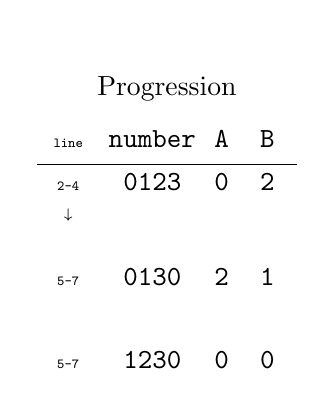
\begin{tikzpicture}[
				value/.style={font=\ttfamily},
				leading/.style={value, inner xsep=8pt, xshift=2pt},
				indicator/.style={inner sep=0, font=\ttfamily\scriptsize},
				line/.style={inner sep=6pt, font=\ttfamily\tiny}]
		
				\node (title) {Progression};
		
				\matrix (progress)  [
					below=0em of title,
					matrix of nodes, 
					column 1/.style={line},
					column 2/.style={value},
					column 3/.style={value},
					column 4/.style={leading}] {
		
					line & number & A & B \\
					\hline
		
					2-4 & 0123 & 0 & 2 \\[-1.3ex]
					$\downarrow$ & ~~~~~ & & \\[0.8em]
		
					5-7 & 0130 & 2 & 1 \\[-1.3ex]
					$\circlearrowright$ & ~~~~~ & & \\[0.8em]
		
					5-7 & 1230 & 0 & 0 \\[-1.3ex]
					$\circlearrowright$ & ~~~~~ & & \\
				};
		
				\ByteIndicator{3};
				\ByteIndicator{5};
				\ByteIndicator{7};
		
				\HLindicator{3}{3.15ex};
				\HLindicator{5}{0.8ex};
				\HLindicator{7}{-1.45ex};
		
			\end{tikzpicture}
	
		\end{tabular}

		\begin{DetailEffects}[p]
			\FlagsRLD
		\end{DetailEffects}
						
		\begin{DetailTiming}
			\DetailTime{5}{18}
		\end{DetailTiming}

		\DetailNote{Note: instruction doesn't assume any format of the data; it simply rotates nibbles. So while it's most frequently associated with BCD numbers, it can be used for shifting hexadecimal values or any other content.}

	\end{DetailItem}

	%----------------------------------------------------------------------------------------------------------------------
	% ███████████████████████████████████████████████████████████████████
	% █▄─▄█▄─▀█▄─▄█─▄▄▄▄█─▄─▄─█▄─▄▄▀█▄─██─▄█─▄▄▄─█─▄─▄─█▄─▄█─▄▄─█▄─▀█▄─▄█
	% ██─███─█▄▀─██▄▄▄▄─███─████─▄─▄██─██─██─███▀███─████─██─██─██─█▄▀─██
	% ▀▄▄▄▀▄▄▄▀▀▄▄▀▄▄▄▄▄▀▀▄▄▄▀▀▄▄▀▄▄▀▀▄▄▄▄▀▀▄▄▄▄▄▀▀▄▄▄▀▀▄▄▄▀▄▄▄▄▀▄▄▄▀▀▄▄▀
	%----------------------------------------------------------------------------------------------------------------------

	\begin{DetailItem}{RRCA}{}
		{\IH{R}otate \IH{R}ight \IH{C}ircular \IH{A}ccumulator}
		{\SymRRC{A}}

		Performs {\tt RRC A}, but twice faster and preserves \FlagSF{}, \FlagZF{} and \FlagPV{}.

		\begin{DetailEffects}
			\FlagsRRCA
		\end{DetailEffects}

		\begin{DetailEffectsFlags}
			\DetailFlagCF[set to:]{bit {\tt 0} of the original value}
		\end{DetailEffectsFlags}

		\begin{DetailTiming}
			\DetailTime{1}{4}
		\end{DetailTiming}

	\end{DetailItem}

	\pagebreak

	%----------------------------------------------------------------------------------------------------------------------
	% ███████████████████████████████████████████████████████████████████
	% █▄─▄█▄─▀█▄─▄█─▄▄▄▄█─▄─▄─█▄─▄▄▀█▄─██─▄█─▄▄▄─█─▄─▄─█▄─▄█─▄▄─█▄─▀█▄─▄█
	% ██─███─█▄▀─██▄▄▄▄─███─████─▄─▄██─██─██─███▀███─████─██─██─██─█▄▀─██
	% ▀▄▄▄▀▄▄▄▀▀▄▄▀▄▄▄▄▄▀▀▄▄▄▀▀▄▄▀▄▄▀▀▄▄▄▄▀▀▄▄▄▄▄▀▀▄▄▄▀▀▄▄▄▀▄▄▄▄▀▄▄▄▀▀▄▄▀
	%----------------------------------------------------------------------------------------------------------------------

	\begin{DetailItem}{RRD}{}
		{\IH{R}otate \IH{R}ight bcd \IH{D}igit}
		{\SymRRD}
		
		Similar to {\tt RLD} except rotation is to the right. If used with BCD values, this operation effectively divides 3-digit BCD number by {\tt 10} and stores remainder in {\tt A}. Taking the example from {\tt RLD}, we can easily convert it to division by 10 simply by using {\tt RRD}. Note however we also need to change the order - we start from MSB now (which is exactly how division would be performed by hand):

		\begin{tabular}{m{8cm}p{0.1cm}m{4.3cm}}

			{ % tcblisting must be enclosed within {} inside tabular otherwise latex compiler gets confused
			\begin{tcblisting}{}
DivideBy10:
	LD HL, number	; number=0123
	LD B, digits	; number of repeats
	XOR A			; reset "carry"
lp:	RRD				; divide by 10 
	INC HL			; next 2 digits
	DJNZ lp			; number=0012, A=3

number:
	DB &01, &23
digits = &-number   ;(2)
			\end{tcblisting}
			}
	
			& &
   	
			\newcommand{\HLindicator}[2]{
				\path (progress-#1-2.south west) --
					node[xshift=#2, yshift=1.4ex, rotate=90]{$\lbrace$}
					node[xshift=#2 + 0.1ex, yshift=0.2ex, indicator]{(HL)} (progress-#1-2.south)
			}

			\newcommand{\ByteIndicator}[1]{
				\draw 
					(progress-#1-2.south west) ++(8pt,13pt) 
					|- ++(5pt,-3pt) -| ++(5pt,3pt) 
					++(1pt,0) 
					|- ++(5pt,-3pt) -| ++(5pt,3pt);
			}
	
			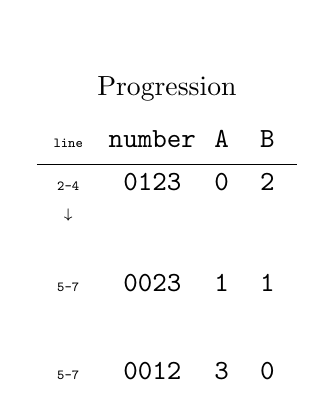
\begin{tikzpicture}[
				value/.style={font=\ttfamily},
				leading/.style={value, inner xsep=8pt, xshift=2pt},
				indicator/.style={inner sep=0, font=\ttfamily\scriptsize},
				line/.style={inner sep=6pt, font=\ttfamily\tiny}]
	
				\node (title) {Progression};
	
				\matrix (progress)  [
					below=0em of title,
					matrix of nodes, 
					column 1/.style={line},
					column 2/.style={value},
					column 3/.style={value},
					column 4/.style={leading}] {

					line & number & A & B \\
					\hline

					2-4 & 0123 & 0 & 2 \\[-1.3ex]
					$\downarrow$ & ~~~~~ & & \\[1em]

					5-7 & 0023 & 1 & 1 \\[-1.3ex]
					$\circlearrowright$ & ~~~~~ & & \\[1em]

					5-7 & 0012 & 3 & 0 \\[-1.3ex]
					$\circlearrowright$ & ~~~~~  & \\[1em]
				};
	
				\ByteIndicator{3};
				\ByteIndicator{5};
				\ByteIndicator{7};
		
				\HLindicator{3}{0.8ex};
				\HLindicator{5}{3.15ex};
				\HLindicator{7}{5.6ex};
	
			\end{tikzpicture}	

		\end{tabular}
		
		\begin{DetailEffects}[p]
			\FlagsRRD
		\end{DetailEffects}
						
		\begin{DetailTiming}
			\DetailTime{5}{18}
		\end{DetailTiming}

		\DetailNote{Note: similar to {\tt RLD}, this instruction also doesn't assume any format of the data; it simply rotates nibbles. So while it's most frequently associated with BCD numbers, it can be used for shifting hexadecimal values or any other content.}

	\end{DetailItem}

	\pagebreak

	%----------------------------------------------------------------------------------------------------------------------
	% ███████████████████████████████████████████████████████████████████
	% █▄─▄█▄─▀█▄─▄█─▄▄▄▄█─▄─▄─█▄─▄▄▀█▄─██─▄█─▄▄▄─█─▄─▄─█▄─▄█─▄▄─█▄─▀█▄─▄█
	% ██─███─█▄▀─██▄▄▄▄─███─████─▄─▄██─██─██─███▀███─████─██─██─██─█▄▀─██
	% ▀▄▄▄▀▄▄▄▀▀▄▄▀▄▄▄▄▄▀▀▄▄▄▀▀▄▄▀▄▄▀▀▄▄▄▄▀▀▄▄▄▄▄▀▀▄▄▄▀▀▄▄▄▀▄▄▄▄▀▄▄▄▀▀▄▄▀
	%----------------------------------------------------------------------------------------------------------------------

	\begin{DetailItem}{RST}{n}
		{\IH{R}e\IH{ST}art}
		{\SymRST{n}}

		\begin{DetailVariants}
			RST \$00\\
			RST \$08\\
			RST \$10\\
			RST \$18
			
			\columnbreak
			RST \$20\\
			RST \$28\\
			RST \$30\\
			RST \$38
		\end{DetailVariants}

		Restarts at the zero page address {\tt s}. Only above addresses are possible, all in page {\tt 0} of the memory, therefore the most significant byte of the program counter {\tt PC} is loaded with {\tt \$00}. The instruction may be used as a fast response to an interrupt.

		\begin{DetailEffects}
			\FlagsRSTn				
		\end{DetailEffects}

		\begin{DetailTiming}
			\DetailTime{3}{11}
		\end{DetailTiming}

	\end{DetailItem}

	% SBC should be listed here alphabetically, but we move it backwards so we can have both SBC and SUB on the same page spread for easier comparison
	\DetailItemSeePageReference{SBC}

	%----------------------------------------------------------------------------------------------------------------------
	% ███████████████████████████████████████████████████████████████████
	% █▄─▄█▄─▀█▄─▄█─▄▄▄▄█─▄─▄─█▄─▄▄▀█▄─██─▄█─▄▄▄─█─▄─▄─█▄─▄█─▄▄─█▄─▀█▄─▄█
	% ██─███─█▄▀─██▄▄▄▄─███─████─▄─▄██─██─██─███▀███─████─██─██─██─█▄▀─██
	% ▀▄▄▄▀▄▄▄▀▀▄▄▀▄▄▄▄▄▀▀▄▄▄▀▀▄▄▀▄▄▀▀▄▄▄▄▀▀▄▄▄▄▄▀▀▄▄▄▀▀▄▄▄▀▄▄▄▄▀▄▄▄▀▀▄▄▀
	%----------------------------------------------------------------------------------------------------------------------

	\begin{DetailItem}{SCF}{}
		{\IH{S}et \IH{C}arry \IH{F}lag}
		{\SymSCF}

		Sets carry flag \FlagCF{}.

		\begin{DetailEffects}
			\FlagsSCF
		\end{DetailEffects}
						
		\begin{DetailTiming}
			\DetailTime{1}{4}
		\end{DetailTiming}

	\end{DetailItem}

	\pagebreak

	%----------------------------------------------------------------------------------------------------------------------
	% ███████████████████████████████████████████████████████████████████
	% █▄─▄█▄─▀█▄─▄█─▄▄▄▄█─▄─▄─█▄─▄▄▀█▄─██─▄█─▄▄▄─█─▄─▄─█▄─▄█─▄▄─█▄─▀█▄─▄█
	% ██─███─█▄▀─██▄▄▄▄─███─████─▄─▄██─██─██─███▀███─████─██─██─██─█▄▀─██
	% ▀▄▄▄▀▄▄▄▀▀▄▄▀▄▄▄▄▄▀▀▄▄▄▀▀▄▄▀▄▄▀▀▄▄▄▄▀▀▄▄▄▄▄▀▀▄▄▄▀▀▄▄▄▀▄▄▄▄▀▄▄▄▀▀▄▄▀
	%----------------------------------------------------------------------------------------------------------------------

	\begin{DetailItem}{SET}{b,s}
		{\IH{SET} bit}
		{\SymSET{s}}

		\begin{DetailVariants}
			SET b,A\\
			SET b,B\\
			SET b,C\\
			SET b,D\\
			SET b,E\\
			SET b,H\\
			SET b,L\\
			SET b,(HL)\\
			SET b,(IX+d)\\
			SET b,(IY+d)

			\columnbreak
			SET b,(IX+d),A\UNDOC\\
			SET b,(IX+d),B\UNDOC\\
			SET b,(IX+d),C\UNDOC\\
			SET b,(IX+d),D\UNDOC\\
			SET b,(IX+d),E\UNDOC\\
			SET b,(IX+d),H\UNDOC\\
			SET b,(IX+d),L\UNDOC

			\columnbreak
			SET b,(IY+d),A\UNDOC\\
			SET b,(IY+d),B\UNDOC\\
			SET b,(IY+d),C\UNDOC\\
			SET b,(IY+d),D\UNDOC\\
			SET b,(IY+d),E\UNDOC\\
			SET b,(IY+d),H\UNDOC\\
			SET b,(IY+d),L\UNDOC
		\end{DetailVariants}

		Sets bit {\tt b} ({\tt 0-7}) of operand {\tt s} or memory location addressed by {\tt s}.

		Note: undocumented variants work slightly differently:

		\begin{multicols}{2}
			\DetailSymbolVariants{SET b,(IX+d),r}{\SymSETu{r}{IX}}

			\DetailSymbolVariants{SET b,(IY+d),r}{\SymSETu{r}{IY}}
		\end{multicols}

		\begin{DetailEffects}
			\FlagsSETr
		\end{DetailEffects}

		\begin{DetailTiming}
			\DetailTime[r]{2}{8}
			\DetailTime[(HL)]{4}{15}
			\DetailTime[(IX+d)]{6}{23}
			\DetailTime[(IY+d)]{6}{23}
		\end{DetailTiming}

	\end{DetailItem}

	%----------------------------------------------------------------------------------------------------------------------
	% ███████████████████████████████████████████████████████████████████
	% █▄─▄█▄─▀█▄─▄█─▄▄▄▄█─▄─▄─█▄─▄▄▀█▄─██─▄█─▄▄▄─█─▄─▄─█▄─▄█─▄▄─█▄─▀█▄─▄█
	% ██─███─█▄▀─██▄▄▄▄─███─████─▄─▄██─██─██─███▀███─████─██─██─██─█▄▀─██
	% ▀▄▄▄▀▄▄▄▀▀▄▄▀▄▄▄▄▄▀▀▄▄▄▀▀▄▄▀▄▄▀▀▄▄▄▄▀▀▄▄▄▄▄▀▀▄▄▄▀▀▄▄▄▀▄▄▄▄▀▄▄▄▀▀▄▄▀
	%----------------------------------------------------------------------------------------------------------------------

	\begin{DetailItem}{SETAE}{\DetailItemZXN}
		{\IH{SET} \IH{A}ccumulator from \IH{E}}
		{\SymSETAE}

		Takes the bit number to set from {\tt E} (only the low 3 bits) and sets the value of the accumulator {\tt A} to the value of that bit, but counted from top to bottom ({\tt E=0} will produce {\tt A$\leftarrow$\$80}, {\tt E=7} will produce {\tt A$\leftarrow$\$01} and so on). This works as pixel mask for ULA bitmap modes, when {\tt E} represents x-coordinate {\tt 0-255}.

		\begin{DetailEffects}
			\FlagsSETAE
		\end{DetailEffects}
						
		\begin{DetailTiming}
			\DetailTime{2}{8}
		\end{DetailTiming}

	\end{DetailItem}

	\pagebreak

	%----------------------------------------------------------------------------------------------------------------------
	% ███████████████████████████████████████████████████████████████████
	% █▄─▄█▄─▀█▄─▄█─▄▄▄▄█─▄─▄─█▄─▄▄▀█▄─██─▄█─▄▄▄─█─▄─▄─█▄─▄█─▄▄─█▄─▀█▄─▄█
	% ██─███─█▄▀─██▄▄▄▄─███─████─▄─▄██─██─██─███▀███─████─██─██─██─█▄▀─██
	% ▀▄▄▄▀▄▄▄▀▀▄▄▀▄▄▄▄▄▀▀▄▄▄▀▀▄▄▀▄▄▀▀▄▄▄▄▀▀▄▄▄▄▄▀▀▄▄▄▀▀▄▄▄▀▄▄▄▄▀▄▄▄▀▀▄▄▀
	%----------------------------------------------------------------------------------------------------------------------

	\begin{DetailItem}{SLA}{s}
		{\IH{S}hift \IH{L}eft \IH{A}rithmetic}
		{\SymSLA{s}}
		
		\begin{DetailVariants}
			SLA A\\
			SLA B\\
			SLA C\\
			SLA D\\
			SLA E\\
			SLA H\\
			SLA L\\
			SLA (HL)\\
			SLA (IX+d)\\
			SLA (IY+d)

			\columnbreak
			SLA (IX+d),A\UNDOC\\
			SLA (IX+d),B\UNDOC\\
			SLA (IX+d),C\UNDOC\\
			SLA (IX+d),D\UNDOC\\
			SLA (IX+d),E\UNDOC\\
			SLA (IX+d),H\UNDOC\\
			SLA (IX+d),L\UNDOC

			\columnbreak
			SLA (IY+d),A\UNDOC\\
			SLA (IY+d),B\UNDOC\\
			SLA (IY+d),C\UNDOC\\
			SLA (IY+d),D\UNDOC\\
			SLA (IY+d),E\UNDOC\\
			SLA (IY+d),H\UNDOC\\
			SLA (IY+d),L\UNDOC
		\end{DetailVariants}

		Performs arithmetic shift left of the operand {\tt s} or memory location addressed by {\tt s}. Bit {\tt 0} is forced to {\tt 0} and bit {\tt 7} is moved to \FlagCF{}.

		\begin{DetailEffects}[p]
			\FlagsSLAr
		\end{DetailEffects}

		\begin{DetailEffectsFlags}
			\DetailFlagSF{\DetailFlagResultSign}
			\DetailFlagZF{\DetailFlagResultZero}
			\DetailFlagPV{\DetailFlagResultParity}
			\DetailFlagCF[set to:]{bit 7 of the original value}
		\end{DetailEffectsFlags}

		\begin{DetailTiming}
			\DetailTime[r]{2}{8}
			\DetailTime[(HL)]{4}{15}
			\DetailTime[(IX+d)]{6}{23}
			\DetailTime[(IY+d)]{6}{23}
		\end{DetailTiming}

	\end{DetailItem}

	%----------------------------------------------------------------------------------------------------------------------
	% ███████████████████████████████████████████████████████████████████
	% █▄─▄█▄─▀█▄─▄█─▄▄▄▄█─▄─▄─█▄─▄▄▀█▄─██─▄█─▄▄▄─█─▄─▄─█▄─▄█─▄▄─█▄─▀█▄─▄█
	% ██─███─█▄▀─██▄▄▄▄─███─████─▄─▄██─██─██─███▀███─████─██─██─██─█▄▀─██
	% ▀▄▄▄▀▄▄▄▀▀▄▄▀▄▄▄▄▄▀▀▄▄▄▀▀▄▄▀▄▄▀▀▄▄▄▄▀▀▄▄▄▄▄▀▀▄▄▄▀▀▄▄▄▀▄▄▄▄▀▄▄▄▀▀▄▄▀
	%----------------------------------------------------------------------------------------------------------------------

	\begin{DetailItem}{SLL}{}
		{\IH{S}hift \IH{L}eft \IH{L}ogical}
		{}

		This mnemonic has no associated opcode on Next. There is no difference between logical and arithmetic shift left, use {\tt SLA} for both. Some assemblers will allow {\tt SLL} as equivalent, but unfortunately, some will assemble it as {\tt SLI}, so it's best avoiding.
		
	\end{DetailItem}

	\pagebreak

	%----------------------------------------------------------------------------------------------------------------------
	% ███████████████████████████████████████████████████████████████████
	% █▄─▄█▄─▀█▄─▄█─▄▄▄▄█─▄─▄─█▄─▄▄▀█▄─██─▄█─▄▄▄─█─▄─▄─█▄─▄█─▄▄─█▄─▀█▄─▄█
	% ██─███─█▄▀─██▄▄▄▄─███─████─▄─▄██─██─██─███▀███─████─██─██─██─█▄▀─██
	% ▀▄▄▄▀▄▄▄▀▀▄▄▀▄▄▄▄▄▀▀▄▄▄▀▀▄▄▀▄▄▀▀▄▄▄▄▀▀▄▄▄▄▄▀▀▄▄▄▀▀▄▄▄▀▄▄▄▄▀▄▄▄▀▀▄▄▀
	%----------------------------------------------------------------------------------------------------------------------

	\begin{DetailItemMultiline}
		{SLI}{s\UNDOC}{\IH{S}hift \IH{L}eft and \IH{I}ncrement}
		{SL1}{s\UNDOC}{\IH{S}hift \IH{L}eft and add \IH{1}}
		{\SymSLI{s}}
		
		\begin{DetailVariants}
			SLI A\\
			SLI B\\
			SLI C\\
			SLI D\\
			SLI E\\
			SLI H\\
			SLI L\\
			SLA (HL)\\
			SLA (IX+d)\\
			SLA (IY+d)

			\columnbreak
			SLI (IX+d),A\UNDOC\\
			SLI (IX+d),B\UNDOC\\
			SLI (IX+d),C\UNDOC\\
			SLI (IX+d),D\UNDOC\\
			SLI (IX+d),E\UNDOC\\
			SLI (IX+d),H\UNDOC\\
			SLI (IX+d),L\UNDOC

			\columnbreak
			SLI (IY+d),A\UNDOC\\
			SLI (IY+d),B\UNDOC\\
			SLI (IY+d),C\UNDOC\\
			SLI (IY+d),D\UNDOC\\
			SLI (IY+d),E\UNDOC\\
			SLI (IY+d),H\UNDOC\\
			SLI (IY+d),L\UNDOC
		\end{DetailVariants}

		Undocumented instruction. Similar to {\tt SLA} except {\tt 1} is moved to bit {\tt 0}.

		\begin{DetailEffects}[p]
			\FlagsSLIr
		\end{DetailEffects}

		\begin{DetailEffectsFlags}
			\DetailFlagSF{\DetailFlagResultSign}
			\DetailFlagZF{\DetailFlagResultZero}
			\DetailFlagPV{\DetailFlagResultParity}
			\DetailFlagCF[set to:]{bit 7 of the original value}
		\end{DetailEffectsFlags}

		\begin{DetailTiming}
			\DetailTime[r]{2}{8}
			\DetailTime[(HL)]{4}{15}
			\DetailTime[(IX+d)]{6}{23}
			\DetailTime[(IY+d)]{6}{23}
		\end{DetailTiming}

		\DetailNote{Note: most assemblers will accept both variants: {\tt SLI} or {\tt SL1}, but some may only accept one or the other, while some may expect {\tt SLL} instead.}

	\end{DetailItemMultiline}

	\pagebreak

	%----------------------------------------------------------------------------------------------------------------------
	% ███████████████████████████████████████████████████████████████████
	% █▄─▄█▄─▀█▄─▄█─▄▄▄▄█─▄─▄─█▄─▄▄▀█▄─██─▄█─▄▄▄─█─▄─▄─█▄─▄█─▄▄─█▄─▀█▄─▄█
	% ██─███─█▄▀─██▄▄▄▄─███─████─▄─▄██─██─██─███▀███─████─██─██─██─█▄▀─██
	% ▀▄▄▄▀▄▄▄▀▀▄▄▀▄▄▄▄▄▀▀▄▄▄▀▀▄▄▀▄▄▀▀▄▄▄▄▀▀▄▄▄▄▄▀▀▄▄▄▀▀▄▄▄▀▄▄▄▄▀▄▄▄▀▀▄▄▀
	%----------------------------------------------------------------------------------------------------------------------

	\begin{DetailItem}{SRA}{s}
		{\IH{S}hift \IH{R}ight \IH{A}rithmetic}
		{\SymSRA{s}}
				
		% we're using non-standard layout here so that we can fit SRA and SRL to the same page
		\begin{DetailVariants}[p{1.3cm}p{3.5cm}XX]
			SRA A	& SRA (HL)		& SRA (IX+d),A\UNDOC	& SRA (IY+d),A\UNDOC \\
			SRA B	& SRA (IX+d)	& SRA (IX+d),B\UNDOC	& SRA (IY+d),B\UNDOC \\
			SRA C	& SRA (IY+d)	& SRA (IX+d),C\UNDOC	& SRA (IY+d),C\UNDOC \\
			SRA D	&				& SRA (IX+d),D\UNDOC	& SRA (IY+d),D\UNDOC \\
			SRA E	&				& SRA (IX+d),E\UNDOC	& SRA (IY+d),E\UNDOC \\
			SRA H	&				& SRA (IX+d),H\UNDOC	& SRA (IY+d),H\UNDOC \\
			SRA L	&				& SRA (IX+d),L\UNDOC	& SRA (IY+d),L\UNDOC \\
		\end{DetailVariants}

		Performs arithmetic shift right of the operand {\tt s} or memory location addressed by {\tt s}. Bit {\tt 0} is moved to \FlagCF{} while bit {\tt 7} remains unchanged (on the assumption that it's the sign bit).

		\begin{DetailEffects}[p]
			\FlagsSRAr
		\end{DetailEffects}

		\begin{DetailEffectsFlags}
			\DetailFlagSF{\DetailFlagResultSign}
			\DetailFlagZF{\DetailFlagResultZero}
			\DetailFlagPV{\DetailFlagResultParity}
			\DetailFlagCF[set to:]{bit 0 of the original value}
		\end{DetailEffectsFlags}

		\begin{DetailTiming}
			\DetailTime[r]{2}{8}
			\DetailTime[(HL)]{4}{15}
			\DetailTime[(IX+d)]{6}{23}
			\DetailTime[(IY+d)]{6}{23}
		\end{DetailTiming}

	\end{DetailItem}

	\pagebreak

	%----------------------------------------------------------------------------------------------------------------------
	% ███████████████████████████████████████████████████████████████████
	% █▄─▄█▄─▀█▄─▄█─▄▄▄▄█─▄─▄─█▄─▄▄▀█▄─██─▄█─▄▄▄─█─▄─▄─█▄─▄█─▄▄─█▄─▀█▄─▄█
	% ██─███─█▄▀─██▄▄▄▄─███─████─▄─▄██─██─██─███▀███─████─██─██─██─█▄▀─██
	% ▀▄▄▄▀▄▄▄▀▀▄▄▀▄▄▄▄▄▀▀▄▄▄▀▀▄▄▀▄▄▀▀▄▄▄▄▀▀▄▄▄▄▄▀▀▄▄▄▀▀▄▄▄▀▄▄▄▄▀▄▄▄▀▀▄▄▀
	%----------------------------------------------------------------------------------------------------------------------

	\begin{DetailItem}{SRL}{s}
		{\IH{S}hift \IH{R}ight \IH{L}ogical}
		{\SymSRL{s}}
				
		% we're using non-standard layout here so that we can fit SRA and SRL to the same page
		\begin{DetailVariants}[p{1.3cm}p{3.5cm}XX]
			SRL A	& SRL (HL)		& SRL (IX+d),A\UNDOC	& SRL (IY+d),A\UNDOC \\
			SRL B	& SRL (IX+d)	& SRL (IX+d),B\UNDOC	& SRL (IY+d),B\UNDOC \\
			SRL C	& SRL (IY+d)	& SRL (IX+d),C\UNDOC	& SRL (IY+d),C\UNDOC \\
			SRL D	&				& SRL (IX+d),D\UNDOC	& SRL (IY+d),D\UNDOC \\
			SRL E	&				& SRL (IX+d),E\UNDOC	& SRL (IY+d),E\UNDOC \\
			SRL H	&				& SRL (IX+d),H\UNDOC	& SRL (IY+d),H\UNDOC \\
			SRL L	&				& SRL (IX+d),L\UNDOC	& SRL (IY+d),L\UNDOC \\
		\end{DetailVariants}

		Performs logical shift right of the operand {\tt s} or memory location addressed by {\tt s}. Bit {\tt 0} is moved to \FlagCF{} while {\tt 0} is moved to bit {\tt 7}.

		\begin{DetailEffects}[p]
			\FlagsSRLr
		\end{DetailEffects}

		\begin{DetailEffectsFlags}
			\DetailFlagSF{\DetailFlagResultSign}
			\DetailFlagZF{\DetailFlagResultZero}
			\DetailFlagPV{\DetailFlagResultParity}
			\DetailFlagCF[set to:]{bit 0 of the original value}
		\end{DetailEffectsFlags}

		\begin{DetailTiming}
			\DetailTime[r]{2}{8}
			\DetailTime[(HL)]{4}{15}
			\DetailTime[(IX+d)]{6}{23}
			\DetailTime[(IY+d)]{6}{23}
		\end{DetailTiming}

	\end{DetailItem}

	\pagebreak

	%----------------------------------------------------------------------------------------------------------------------
	% ███████████████████████████████████████████████████████████████████
	% █▄─▄█▄─▀█▄─▄█─▄▄▄▄█─▄─▄─█▄─▄▄▀█▄─██─▄█─▄▄▄─█─▄─▄─█▄─▄█─▄▄─█▄─▀█▄─▄█
	% ██─███─█▄▀─██▄▄▄▄─███─████─▄─▄██─██─██─███▀███─████─██─██─██─█▄▀─██
	% ▀▄▄▄▀▄▄▄▀▀▄▄▀▄▄▄▄▄▀▀▄▄▄▀▀▄▄▀▄▄▀▀▄▄▄▄▀▀▄▄▄▄▄▀▀▄▄▄▀▀▄▄▄▀▄▄▄▄▀▄▄▄▀▀▄▄▀
	%----------------------------------------------------------------------------------------------------------------------

	\begin{DetailItem}{SBC}{d,s}
		{\IH{S}u\IH{B}tract with \IH{C}arry}
		{\SymSBC{d}{s}}
	
		\begin{DetailVariants}
			\textnormal{8 bit}\\
			SBC A,A\\
			SBC A,B\\
			SBC A,C\\
			SBC A,D\\
			SBC A,E\\
			SBC A,H\\
			SBC A,L\\
			SBC A,n

			\columnbreak
			\textnormal{8 bit}\\
			SBC A,IXH\UNDOC\\
			SBC A,IXL\UNDOC\\
			SBC A,IYH\UNDOC\\
			SBC A,IYL\UNDOC\\
			SBC A,(HL)\\
			SBC A,(IX+d)\\
			SBC A,(IY+d)

			\columnbreak
			\textnormal{16 bit}\\
			SBC HL,BC\\
			SBC HL,DE\\
			SBC HL,HL\\
			SBC HL,SP
		\end{DetailVariants}
		
		Subtracts source operand {\tt s} or contents of the memory location addressed by {\tt s} and carry flag \FlagCF{} from destination {\tt d}. Result is then stored to destination {\tt d}.

		\begin{DetailEffects}[v]
			\FlagsSBCr[8-bit]
			\FlagsSBCrr[16-bit]
		\end{DetailEffects}

		\begin{DetailEffectsFlags}
			\DetailFlagSF{\DetailFlagResultSign}
			\DetailFlagZF{\DetailFlagResultZero}
			\DetailFlagHF{\DetailFlagResultHalfBorrow*}*
			\DetailFlagPV{\DetailFlagResultOverflow}*
			\DetailFlagCF{\DetailFlagResultBorrow*}
		\end{DetailEffectsFlags}

		\begin{DetailTiming}
			\DetailTime[r]{1}{4}
			\DetailTime[n]{2}{7}
			\DetailTime[(HL)]{2}{7}
			\DetailTime[HL,rr]{4}{15}
			\DetailTime[(IX+d)]{5}{19}
			\DetailTime[(IY+d)]{5}{19}
		\end{DetailTiming}

	\end{DetailItem}

	\pagebreak

	%----------------------------------------------------------------------------------------------------------------------
	% ███████████████████████████████████████████████████████████████████
	% █▄─▄█▄─▀█▄─▄█─▄▄▄▄█─▄─▄─█▄─▄▄▀█▄─██─▄█─▄▄▄─█─▄─▄─█▄─▄█─▄▄─█▄─▀█▄─▄█
	% ██─███─█▄▀─██▄▄▄▄─███─████─▄─▄██─██─██─███▀███─████─██─██─██─█▄▀─██
	% ▀▄▄▄▀▄▄▄▀▀▄▄▀▄▄▄▄▄▀▀▄▄▄▀▀▄▄▀▄▄▀▀▄▄▄▄▀▀▄▄▄▄▄▀▀▄▄▄▀▀▄▄▄▀▄▄▄▄▀▄▄▄▀▀▄▄▀
	%----------------------------------------------------------------------------------------------------------------------

	\begin{DetailItem}{SUB}{s}
		{\IH{SUB}tract}
		{\SymSUB{s}}

		\begin{DetailVariants}
			SUB A\\
			SUB B\\
			SUB C\\
			SUB D\\
			SUB E\\
			SUB H\\
			SUB L

			\columnbreak
			SUB n\\
			SUB (HL)\\
			SUB (IX+d)\\
			SUB (IY+d)

			\columnbreak
			SUB IXH\UNDOC\\
			SUB IXL\UNDOC\\
			SUB IYH\UNDOC\\
			SUB IYL\UNDOC
		\end{DetailVariants}

		Subtracts 8-bit immediate value, operand {\tt s} or memory location addressed by {\tt s} from accumulator {\tt A}. Then stores result back to {\tt A}.

		\begin{DetailEffects}[v]
			\FlagsSUBr
		\end{DetailEffects}

		\begin{DetailEffectsFlags}
			\DetailFlagSF{\DetailFlagResultSign}
			\DetailFlagZF{\DetailFlagResultZero}
			\DetailFlagHF{\DetailFlagResultHalfBorrow*}*
			\DetailFlagPV{\DetailFlagResultOverflow}*
			\DetailFlagCF{\DetailFlagResultBorrow*}
		\end{DetailEffectsFlags}

		\begin{DetailTiming}
			\DetailTime[r]{1}{4}
			\DetailTime[n]{2}{7}
			\DetailTime[(HL)]{2}{7}
			\DetailTime[(IX+d)]{5}{19}
			\DetailTime[(IY+d)]{5}{19}
		\end{DetailTiming}

	\end{DetailItem}

	\pagebreak

	%----------------------------------------------------------------------------------------------------------------------
	% ███████████████████████████████████████████████████████████████████
	% █▄─▄█▄─▀█▄─▄█─▄▄▄▄█─▄─▄─█▄─▄▄▀█▄─██─▄█─▄▄▄─█─▄─▄─█▄─▄█─▄▄─█▄─▀█▄─▄█
	% ██─███─█▄▀─██▄▄▄▄─███─████─▄─▄██─██─██─███▀███─████─██─██─██─█▄▀─██
	% ▀▄▄▄▀▄▄▄▀▀▄▄▀▄▄▄▄▄▀▀▄▄▄▀▀▄▄▀▄▄▀▀▄▄▄▄▀▀▄▄▄▄▄▀▀▄▄▄▀▀▄▄▄▀▄▄▄▄▀▄▄▄▀▀▄▄▀
	%----------------------------------------------------------------------------------------------------------------------

	\begin{DetailItem}{SWAPNIB}{\DetailItemZXN}
		{\IH{SWAP} \IH{NIB}bles}
		{\SymSWAPNIB}

		Swaps the high and low nibbles of the accumulator {\tt A}.

		\begin{DetailEffects}
			\FlagsSWAPNIB
		\end{DetailEffects}
						
		\begin{DetailTiming}
			\DetailTime{2}{8}
		\end{DetailTiming}

	\end{DetailItem}

	%----------------------------------------------------------------------------------------------------------------------
	% ███████████████████████████████████████████████████████████████████
	% █▄─▄█▄─▀█▄─▄█─▄▄▄▄█─▄─▄─█▄─▄▄▀█▄─██─▄█─▄▄▄─█─▄─▄─█▄─▄█─▄▄─█▄─▀█▄─▄█
	% ██─███─█▄▀─██▄▄▄▄─███─████─▄─▄██─██─██─███▀███─████─██─██─██─█▄▀─██
	% ▀▄▄▄▀▄▄▄▀▀▄▄▀▄▄▄▄▄▀▀▄▄▄▀▀▄▄▀▄▄▀▀▄▄▄▄▀▀▄▄▄▄▄▀▀▄▄▄▀▀▄▄▄▀▄▄▄▄▀▄▄▄▀▀▄▄▀
	%----------------------------------------------------------------------------------------------------------------------

	\begin{DetailItem}{TEST}{n\ZXN}
		{\IH{TEST}}
		{\SymTEST}

		Similar to {\tt CP} (page \DetailItemPageRef{CP}), but performs an {\tt AND} instead of a subtraction. Again, {\tt AND} is performed between the accumulator {\tt A} and value {\tt n}. Status flags are updated according to the result, but the result is then discarded (value of {\tt A} is not changed).

		\begin{DetailEffects}[p]
			\FlagsTESTn
		\end{DetailEffects}

		\begin{DetailEffectsFlags}
			\DetailFlagSF{\DetailFlagResultSign}
			\DetailFlagZF{\DetailFlagResultZero ~(no bits matched)}
			\DetailFlagPV{\DetailFlagResultParity}
		\end{DetailEffectsFlags}

		\begin{DetailTiming}
			\DetailTime{3}{11}
		\end{DetailTiming}

	\end{DetailItem}

	%----------------------------------------------------------------------------------------------------------------------
	% ███████████████████████████████████████████████████████████████████
	% █▄─▄█▄─▀█▄─▄█─▄▄▄▄█─▄─▄─█▄─▄▄▀█▄─██─▄█─▄▄▄─█─▄─▄─█▄─▄█─▄▄─█▄─▀█▄─▄█
	% ██─███─█▄▀─██▄▄▄▄─███─████─▄─▄██─██─██─███▀███─████─██─██─██─█▄▀─██
	% ▀▄▄▄▀▄▄▄▀▀▄▄▀▄▄▄▄▄▀▀▄▄▄▀▀▄▄▀▄▄▀▀▄▄▄▄▀▀▄▄▄▄▄▀▀▄▄▄▀▀▄▄▄▀▄▄▄▄▀▄▄▄▀▀▄▄▀
	%----------------------------------------------------------------------------------------------------------------------

	\pagebreak
	\begin{DetailItem}{XOR}{s}
		{bitwise e\IH{X}clusive \IH{OR}}
		{\SymXOR{s}}

		\begin{DetailVariants}
			XOR A\\
			XOR B\\
			XOR C\\
			XOR D\\
			XOR E\\
			XOR H\\
			XOR L\\
			XOR n

			\columnbreak
			XOR (HL)\\
			XOR (IX+d)\\
			XOR (IY+d)

			\columnbreak
			XOR IXH\UNDOC\\
			XOR IXL\UNDOC\\
			XOR IYH\UNDOC\\
			XOR IYL\UNDOC
		\end{DetailVariants}
		
		\begin{tabularx}{\linewidth}{@{}Xl}
			Performs exclusive or between accumulator {\tt A} and operand {\tt s} or memory location addressed by {\tt s}. Result is then stored back to {\tt A}. Individual bits are XOR'ed as shown on the right:
	
			&

			\begin{tabular}[t]{cc|c}
				{\tt A} & {\tt s} & Result \\
				\hline
				{\tt 0} & {\tt 0} & {\tt 0} \\
				{\tt 0} & {\tt 1} & {\tt 1} \\
				{\tt 1} & {\tt 0} & {\tt 1} \\
				{\tt 1} & {\tt 1} & {\tt 0} \\
			\end{tabular}

			\\
		\end{tabularx}

		\begin{DetailEffects}[p]
			\FlagsXORr
		\end{DetailEffects}

		\begin{DetailEffectsFlags}
			\DetailFlagSF{\DetailFlagResultSign}
			\DetailFlagZF{\DetailFlagResultZero}
			\DetailFlagPV{\DetailFlagResultParity}
		\end{DetailEffectsFlags}

		\begin{DetailTiming}
			\DetailTime[r]{1}{4}
			\DetailTime[n]{2}{7}
			\DetailTime[(HL)]{2}{7}
			\DetailTime[(IX+d)]{5}{19}
			\DetailTime[(IY+d)]{5}{19}
		\end{DetailTiming}

	\end{DetailItem}

\end{basedescript}



	% ░█▀▀█ ▒█▀▀█ ▒█▀▀█ ▒█▀▀▀ ▒█▄░▒█ ▒█▀▀▄ ▀█▀ ▀▄▒▄▀ 
	% ▒█▄▄█ ▒█▄▄█ ▒█▄▄█ ▒█▀▀▀ ▒█▒█▒█ ▒█░▒█ ▒█░ ░▒█░░ 
	% ▒█░▒█ ▒█░░░ ▒█░░░ ▒█▄▄▄ ▒█░░▀█ ▒█▄▄▀ ▄█▄ ▄▀▒▀▄

	\SetupPageFormattingAppendix

	\include{chapter-instr-sorted-mnemonic}
	\include{chapter-instr-sorted-opcode}
	\include{chapter-bibliography}
	\include{chapter-license}

\end{document}
